% Topic 14: Table in HTML
% Source coverage: HTML table PDF pages 1--16 + modern HTML notes.
% Image চিত্রs are added for concept/exercise views.
% Put concept images in: chapters/Chapter04/topics/images/

\section{Table in HTML}

\begin{learningbox}
এই টপিক শেষে শিক্ষার্থী পারবে:
\begin{itemize}
\item HTML table কী এবং ওয়েবপেজে table কখন ব্যবহার করা হয় তা ব্যাখ্যা করতে।
\item \texttt{<table>}, \texttt{<tr>}, \texttt{<th>}, \texttt{<td>} ও \texttt{<caption>} tag-এর কাজ লিখতে।
\item table-এর row, column ও cell view দেখে শনাক্ত করতে।
\item \texttt{border}, \texttt{width}, \texttt{align}, \texttt{bgcolor}, \texttt{cellspacing} ও \texttt{cellpadding} attribute ব্যবহার করতে।
\item \texttt{rowspan} ও \texttt{colspan} ব্যবহার করে cell merge করতে।
\item table-এর ভিতরে text, formatting, link, image, list ও nested table ব্যবহার করতে।
\item চিত্র দেখে board-style HTML table code লিখতে।
\item পুরনো HSC-style attribute এবং modern CSS alternative-এর পার্থক্য বুঝতে।
\end{itemize}
\end{learningbox}

\subsection{ভূমিকা}

ওয়েবপেজে অনেক সময় তথ্য সারি ও কলাম আকারে দেখাতে হয়। যেমন--রেজাল্ট শিট, ক্লাস রুটিন, পণ্যের মূল্য তালিকা, শিক্ষার্থীর তথ্য, salary sheet, bill summary, admission list, college department report ইত্যাদি। এই ধরনের তথ্য সুন্দরভাবে সাজানোর জন্য HTML-এ \textbf{table} ব্যবহার করা হয়। HSC ICT Chapter 4-এ table একটি খুব গুরুত্বপূর্ণ practical topic, কারণ CQ ও practical question-এ প্রায়ই result table, marks sheet, image-সহ table, hyperlink-সহ table, rowspan-colspan table, nested table ইত্যাদি তৈরি করতে বলা হয়।

\begin{keypointbox}{মূল ধারণা}
HTML table শেখার মূল বিষয় হলো: \textbf{row}, \textbf{column}, \textbf{cell}, \textbf{cell merge} এবং \textbf{cell-এর ভিতরে অন্য HTML element ব্যবহার}। এগুলো ঠিকমতো বুঝলে যেকোনো চিত্র দেখে table code লেখা সহজ হয়।
\end{keypointbox}

\begin{boardbox}{কখন table ব্যবহার করবে}
যে তথ্য row ও column আকারে স্বাভাবিকভাবে সাজানো যায়, সেখানে table ব্যবহার করা উচিত। যেমন--result sheet, routine, price list, marks distribution, contact list, product catalog, admission schedule ইত্যাদি। কিন্তু শুধু page layout সাজানোর জন্য table ব্যবহার করা modern web design-এ ভালো practice নয়; layout-এর জন্য CSS layout ব্যবহার করা ভালো। HSC practical-এ তবে বইয়ের figure অনুযায়ী table code লিখতে হবে।
\end{boardbox}

\begin{keypointbox}{Table বোঝার সহজ ভাষা}
একটি table-কে খাতার ছকের মতো ভাবা যায়। প্রথমে ছকের সারি বা row গুনবে, তারপর প্রতিটি row-তে কয়টি ঘর আছে তা দেখবে। যে ঘরটি heading হিসেবে কাজ করে সেটি সাধারণত \texttt{<th>} দিয়ে লেখা হয়, আর সাধারণ তথ্যের ঘর \texttt{<td>} দিয়ে লেখা হয়। কোনো ঘর যদি পাশের ঘর দখল করে নেয়, সেটি \texttt{colspan}; কোনো ঘর যদি নিচের ঘর দখল করে নেয়, সেটি \texttt{rowspan}।
\end{keypointbox}

\subsection{HTML Table কী?}

\begin{definitionbox}{HTML Table}
HTML document-এ তথ্যকে সারি ও কলাম আকারে প্রদর্শনের জন্য যে কাঠামো ব্যবহার করা হয়, তাকে HTML Table বলে।
\end{definitionbox}

Table মূলত \textbf{tabular data} বা row-column আকারের তথ্য দেখানোর জন্য ব্যবহার করা হয়। একটি table বুঝতে তিনটি বিষয় মনে রাখা দরকার: row, column এবং cell।

\begin{center}
\begin{tabular}{|p{0.22\textwidth}|p{0.58\textwidth}|}
\hline
\textbf{অংশ} & \textbf{অর্থ} \\
\hline
Row & আড়াআড়ি সারি \\
\hline
Column & লম্বালম্বি কলাম \\
\hline
Cell & row ও column মিলিত হয়ে যে ঘর তৈরি হয় \\
\hline
\end{tabular}
\end{center}

\begin{examplebox}{ধারণা}
\noindent
\begin{minipage}[t]{0.56\textwidth}
\vspace{0pt}
\begin{center}
\begin{tabular}{|c|c|c|}
\hline
\textbf{Roll} & \textbf{Name} & \textbf{GPA} \\
\hline
101 & Rafi & 5.00 \\
\hline
102 & Sakib & 4.75 \\
\hline
\end{tabular}
\end{center}
এখানে Roll, Name, GPA হলো heading cell; 101, Rafi, 5.00 হলো data cell; প্রতিটি horizontal line একটি row এবং প্রতিটি vertical section একটি column বোঝায়।

\textbf{চিত্র ব্যাখ্যা:} চিত্রে HTML table-এর row, column এবং cell আলাদা label দিয়ে দেখানো হয়েছে। Row হলো আড়াআড়ি সারি, column হলো লম্বালম্বি অংশ এবং row-column মিলিত হয়ে cell তৈরি করে।
\end{minipage}
\hfill
\begin{minipage}[t]{0.38\textwidth}
\vspace{0pt}
\centering
\IfFileExists{chapters/Chapter04/topics/images/3d_row_column_cell.png}{%
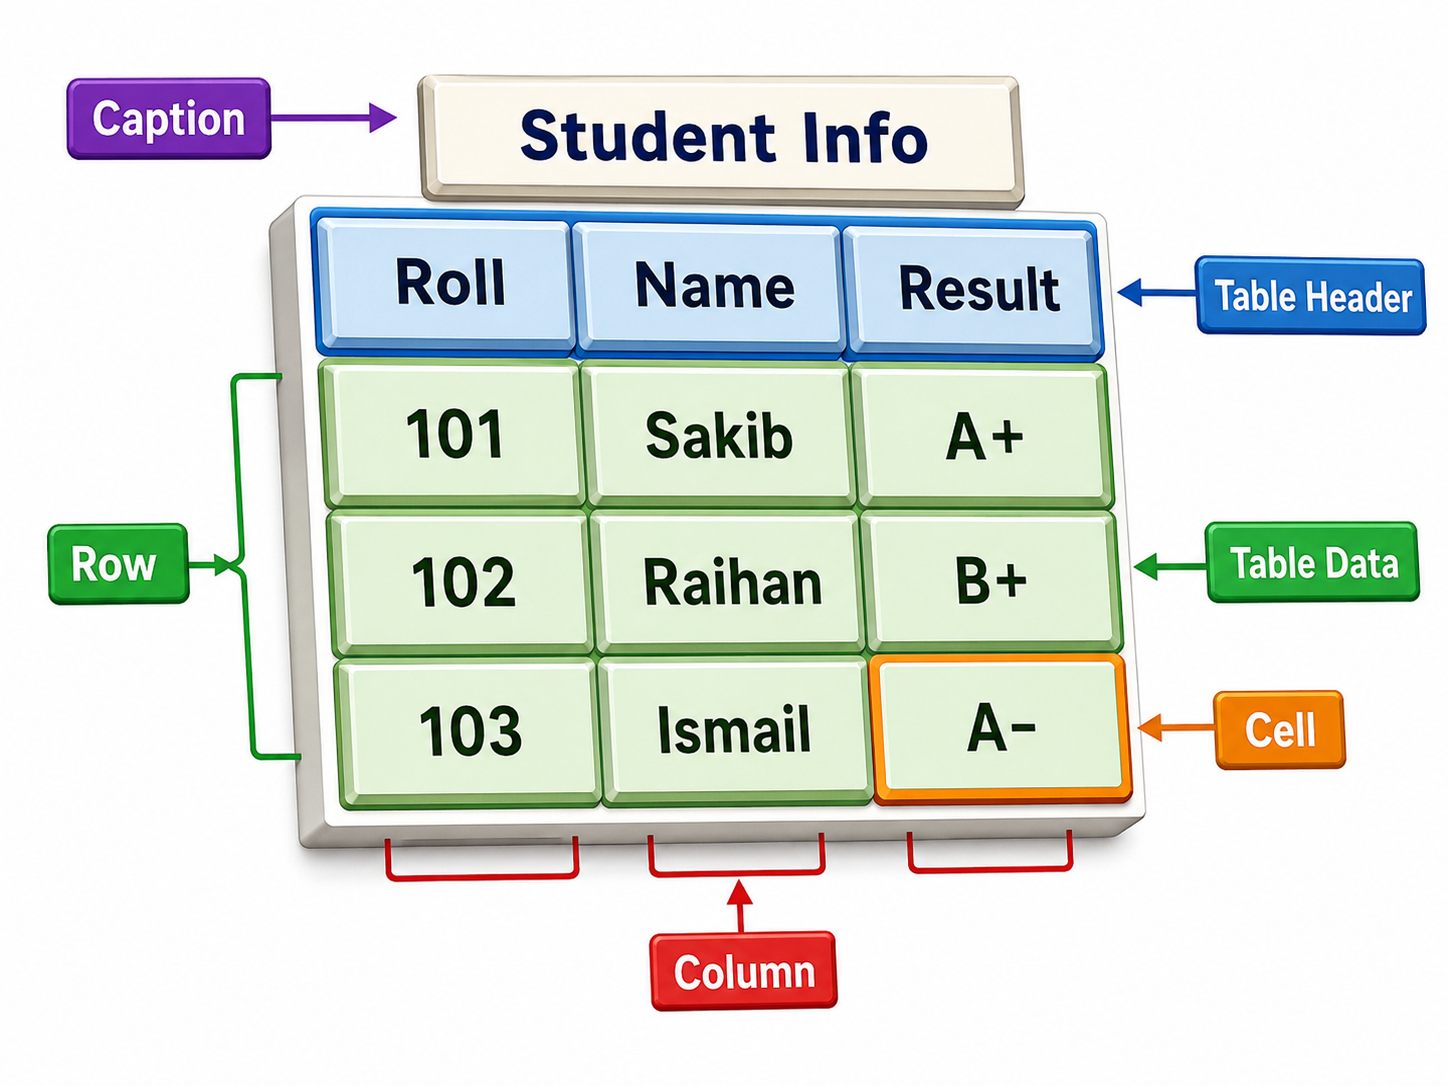
\includegraphics[width=0.98\linewidth,height=0.20\textheight,keepaspectratio]{chapters/Chapter04/topics/images/3d_row_column_cell.png}%
}{%
\fbox{\parbox{0.88\linewidth}{\centering\scriptsize চিত্র পাওয়া যায়নি}}%
}
\par\vspace{1pt}
{\scriptsize\captionof{figure}{HTML table-এর row, column ও cell}}
\end{minipage}
\end{examplebox}


\subsection{Table তৈরির প্রধান Tag}

\noindent
\begin{minipage}[t]{0.56\textwidth}
\vspace{0pt}
\begin{center}
\begin{tabular}{|p{0.22\linewidth}|p{0.24\linewidth}|p{0.34\linewidth}|}
\hline
\textbf{Tag} & \textbf{পূর্ণরূপ/অর্থ} & \textbf{কাজ} \\
\hline
\texttt{<table>} & Table & table শুরু ও শেষ করে \\
\hline
\texttt{<tr>} & Table Row & table-এর row বা সারি তৈরি করে \\
\hline
\texttt{<th>} & Table Header & heading cell তৈরি করে \\
\hline
\texttt{<td>} & Table Data & data cell তৈরি করে \\
\hline
\texttt{<caption>} & Caption & table-এর title বা শিরোনাম দেখায় \\
\hline
\end{tabular}
\end{center}
\textbf{চিত্র ব্যাখ্যা:}
চিত্রে table তৈরির প্রধান tagগুলোর সম্পর্ক দেখানো হয়েছে। \texttt{<table>} পুরো table, \texttt{<tr>} row, \texttt{<th>} heading cell এবং \texttt{<td>} data cell তৈরি করে।
\end{minipage}
\hfill
\begin{minipage}[t]{0.38\textwidth}
\vspace{0pt}
\centering
\IfFileExists{chapters/Chapter04/topics/images/3d_table_tags_map.png}{%
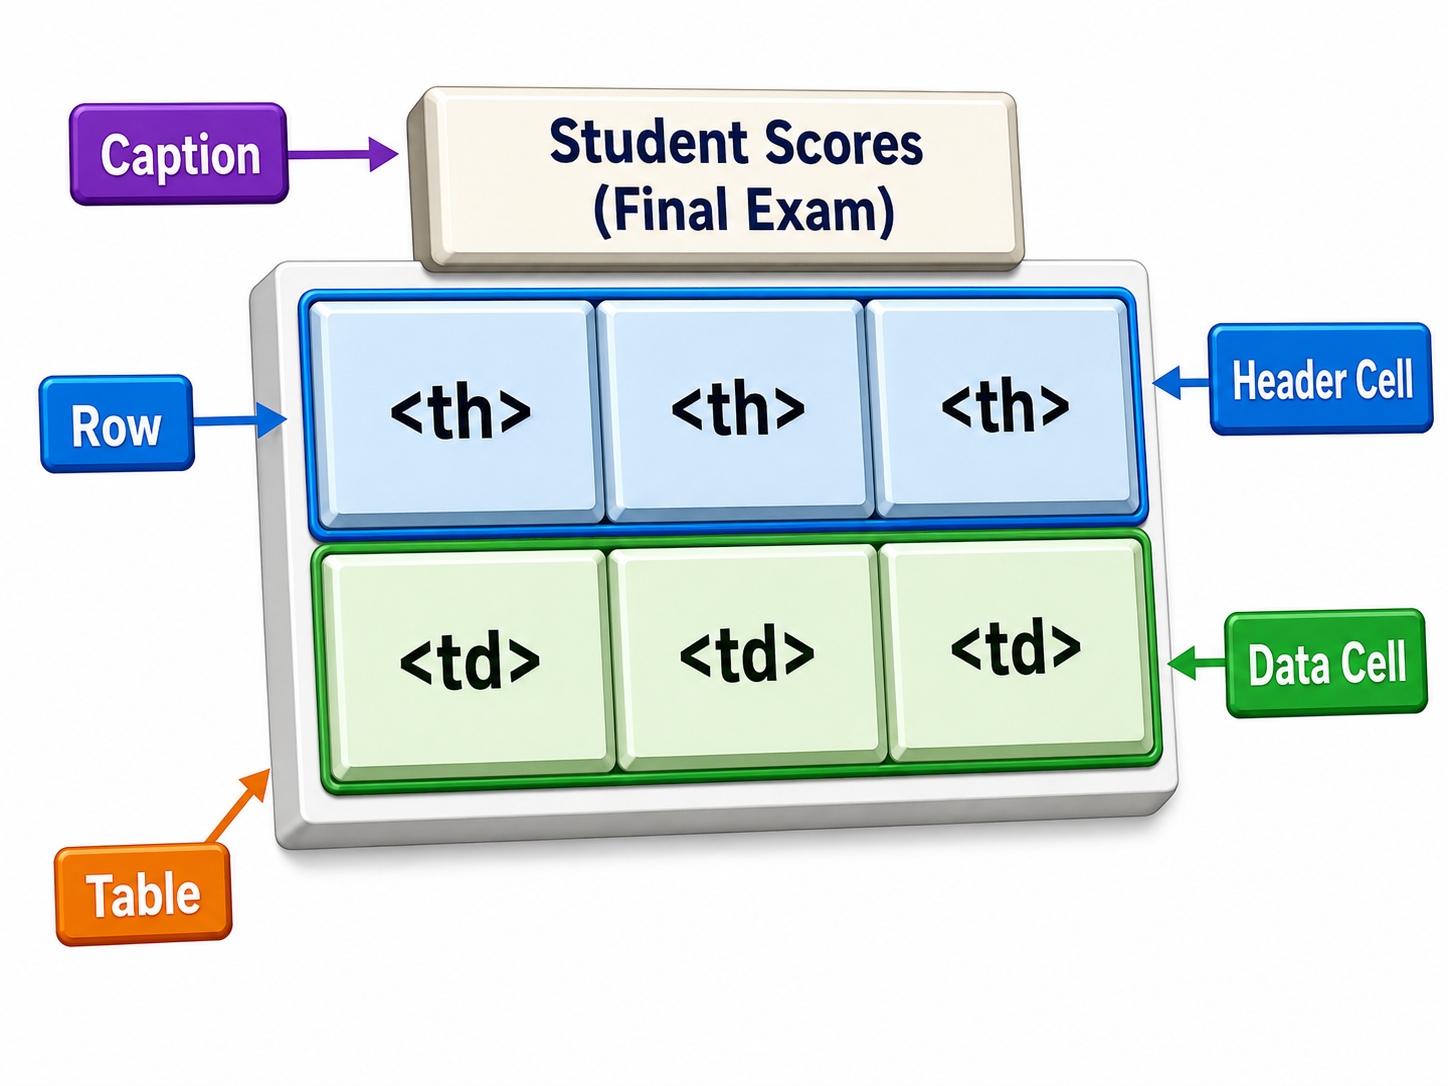
\includegraphics[width=0.98\linewidth,height=0.22\textheight,keepaspectratio]{chapters/Chapter04/topics/images/3d_table_tags_map.png}%
}{%
\fbox{\parbox{0.88\linewidth}{\centering\scriptsize চিত্র পাওয়া যায়নি}}%
}
\par\vspace{1pt}
{\scriptsize\captionof{figure}{table tag-এর কাজ}}
\end{minipage}


\subsection{\texttt{<table>} Tag}

\begin{definitionbox}{\texttt{<table>} tag}
HTML document-এ table বা ছক তৈরি করার জন্য ব্যবহৃত container tag হলো \texttt{<table>} tag।
\end{definitionbox}

Table-এর সব row ও cell এই tag-এর ভিতরে লেখা হয়।

\begin{examplebox}{কোড}
\begin{verbatim}
<!DOCTYPE html>
<html>
<head>
  <title>HTML Table Example</title>
</head>
<body>
  <table border="1" cellspacing="0" cellpadding="6">
    <tr>
      <td>Data</td>
    </tr>
  </table>
</body>
</html>
\end{verbatim}
\end{examplebox}

\subsection{\texttt{<tr>} Tag}

\begin{definitionbox}{\texttt{<tr>} tag}
HTML table-এর একটি row বা সারি তৈরি করার জন্য \texttt{<tr>} tag ব্যবহার করা হয়।
\end{definitionbox}

প্রতিটি \texttt{<tr>} tag-এর ভিতরে এক বা একাধিক \texttt{<th>} অথবা \texttt{<td>} লেখা হয়।

\begin{examplebox}{কোড}
\begin{verbatim}
<!DOCTYPE html>
<html>
<head>
  <title>Table Row Example</title>
</head>
<body>
  <table border="1" cellspacing="0" cellpadding="6">
    <tr>
      <td>Data 1</td>
      <td>Data 2</td>
    </tr>
  </table>
</body>
</html>
\end{verbatim}
\end{examplebox}

\subsection{\texttt{<th>} Tag}

\begin{definitionbox}{\texttt{<th>} tag}
HTML table-এর heading cell তৈরি করার জন্য ব্যবহৃত tag হলো \texttt{<th>} tag।
\end{definitionbox}

Browser সাধারণত \texttt{<th>} tag-এর text bold ও center aligned করে দেখায়।

\begin{examplebox}{কোড}
\begin{verbatim}
<!DOCTYPE html>
<html>
<head>
  <title>Table Header Example</title>
</head>
<body>
  <table border="1" cellspacing="0" cellpadding="6">
    <tr>
      <th>Name</th>
      <th>Roll</th>
    </tr>
  </table>
</body>
</html>
\end{verbatim}
\end{examplebox}

\subsection{\texttt{<td>} Tag}

\begin{definitionbox}{\texttt{<td>} tag}
HTML table-এর data cell বা তথ্যের ঘর তৈরি করার জন্য ব্যবহৃত tag হলো \texttt{<td>} tag।
\end{definitionbox}

\begin{examplebox}{কোড}
\begin{verbatim}
<!DOCTYPE html>
<html>
<head>
  <title>Table Data Example</title>
</head>
<body>
  <table border="1" cellspacing="0" cellpadding="6">
    <tr>
      <td>Rafi</td>
      <td>101</td>
    </tr>
  </table>
</body>
</html>
\end{verbatim}
\end{examplebox}

\subsection{Basic Table Syntax}

\begin{examplebox}{কোড}
\begin{verbatim}
<!DOCTYPE html>
<html>
<head>
  <title>HTML Table Example</title>
</head>
<body>
<table>
  <tr>
    <th>Heading 1</th>
    <th>Heading 2</th>
  </tr>
  <tr>
    <td>Data 1</td>
    <td>Data 2</td>
  </tr>
</table>
</body>
</html>
\end{verbatim}
\end{examplebox}

\begin{keypointbox}{Structure মনে রাখো}
\texttt{<table>} পুরো table তৈরি করে, \texttt{<tr>} একটি row তৈরি করে, \texttt{<th>} heading cell তৈরি করে এবং \texttt{<td>} data cell তৈরি করে।
\end{keypointbox}

\subsection{Table Code লেখার Logical Structure}

HTML table লেখার সময় browser উপর থেকে নিচে row-by-row code পড়ে। তাই code লেখার সময় কোনো cell আগে বা পরে লিখলে visual output বদলে যেতে পারে। একটি row শুরু করতে \texttt{<tr>} লিখতে হয় এবং সেই row-এর যতগুলো cell আছে সেগুলো \texttt{<th>} অথবা \texttt{<td>} দিয়ে একই \texttt{<tr>} tag-এর ভিতরে লিখতে হয়।

\begin{keypointbox}{মনে রাখার নিয়ম}
Table-এর ভিতরে সরাসরি text লেখা উচিত নয়। Table-এর content সাধারণত cell-এর ভিতরে থাকে। তাই correct structure হলো:
\texttt{<table>} $\rightarrow$ \texttt{<tr>} $\rightarrow$ \texttt{<th>} বা \texttt{<td>} $\rightarrow$ content।
\end{keypointbox}

\begin{center}
\begin{tabular}{|p{0.24\textwidth}|p{0.58\textwidth}|}
\hline
\textbf{ধাপ} & \textbf{কাজ} \\
\hline
১ & \texttt{<table>} দিয়ে table শুরু করা \\
\hline
২ & প্রতিটি row-এর জন্য \texttt{<tr>} লেখা \\
\hline
৩ & heading হলে \texttt{<th>}, data হলে \texttt{<td>} লেখা \\
\hline
৪ & সব opened tag ঠিকভাবে close করা \\
\hline
\end{tabular}
\end{center}

\subsection{Simple Table Example}

\begin{examplebox}{কোড}
\begin{verbatim}
<!DOCTYPE html>
<html>
<head>
  <title>Simple Table</title>
</head>
<body>
  <table border="1">
    <tr>
      <th>Roll</th>
      <th>Name</th>
      <th>GPA</th>
    </tr>
    <tr>
      <td>101</td>
      <td>Rafi</td>
      <td>5.00</td>
    </tr>
    <tr>
      <td>102</td>
      <td>Sakib</td>
      <td>4.75</td>
    </tr>
  </table>
</body>
</html>
\end{verbatim}
\end{examplebox}

\begin{examplebox}{Output ধারণা}
\begin{center}
\begin{tabular}{|c|c|c|}
\hline
\textbf{Roll} & \textbf{Name} & \textbf{GPA} \\
\hline
101 & Rafi & 5.00 \\
\hline
102 & Sakib & 4.75 \\
\hline
\end{tabular}
\end{center}
\end{examplebox}

\begin{boardbox}{কোড বিশ্লেষণ}
উপরের code-এ প্রথম \texttt{<tr>} হলো heading row। সেখানে Roll, Name, GPA--এই তিনটি heading cell আছে, তাই \texttt{<th>} ব্যবহার করা হয়েছে। পরের দুইটি row data row, তাই সেখানে \texttt{<td>} ব্যবহার করা হয়েছে। \texttt{border="1"} দেওয়ার কারণে table-এর রেখা দেখা যাচ্ছে।
\end{boardbox}

\subsection{Table Design করার আগে কী ভাববে?}

চিত্র দেখে বা question পড়ে table code লেখার আগে সরাসরি code শুরু না করে কয়েকটি বিষয় ঠিক করতে হয়। এতে ভুল কম হয় এবং \texttt{rowspan}/\texttt{colspan} সহজে বোঝা যায়।

\begin{enumerate}
\item Table-এর title বা caption আছে কি না দেখবে।
\item মোট কয়টি visible column আছে তা গুনবে।
\item মোট কয়টি row আছে তা গুনবে।
\item কোন cell heading আর কোন cell data তা আলাদা করবে।
\item কোনো cell একাধিক column জুড়ে আছে কি না দেখবে।
\item কোনো cell একাধিক row জুড়ে আছে কি না দেখবে।
\item cell-এর ভিতরে text, image, link, list বা nested table আছে কি না দেখবে।
\end{enumerate}

\begin{keypointbox}{পরীক্ষার কৌশল}
কোনো figure জটিল মনে হলে প্রথমে pencil দিয়ে row line ও column line আলাদা করে ভাববে। এরপর merged cell বাদ দিয়ে base grid ধরবে। Base grid বুঝলে \texttt{rowspan} ও \texttt{colspan} বসানো সহজ হয়।
\end{keypointbox}

\subsection{Table Attribute}

PDF-এ table তৈরি করার সময় কয়েকটি attribute বারবার ব্যবহার করা হয়েছে। HSC practical exam-এ এগুলো গুরুত্বপূর্ণ। Table-level attribute যেমন \texttt{border}, \texttt{width}, \texttt{align}, \texttt{cellspacing}, \texttt{cellpadding} পুরো table-এর appearance নিয়ন্ত্রণ করে। আবার cell-level attribute যেমন \texttt{align}, \texttt{valign}, \texttt{bgcolor}, \texttt{rowspan}, \texttt{colspan}, \texttt{width}, \texttt{height} নির্দিষ্ট \texttt{<td>} বা \texttt{<th>} cell-এর আচরণ নিয়ন্ত্রণ করে।

\begin{center}
\begin{tabular}{|p{0.20\textwidth}|p{0.42\textwidth}|p{0.25\textwidth}|}
\hline
\textbf{Attribute} & \textbf{কাজ} & \textbf{Example} \\
\hline
\texttt{border} & table ও cell-এর চারপাশে রেখা দেখায় & \texttt{border="1"} \\
\hline
\texttt{width} & table বা cell-এর প্রস্থ pixel/percentage-এ নির্ধারণ করে & \texttt{width="400"} \\
\hline
\texttt{align} & table বা cell-এর left/right/center position নির্ধারণ করে & \texttt{align="center"} \\
\hline
\texttt{cellspacing} & cell থেকে cell-এর মাঝের বাইরের gap নির্ধারণ করে & \texttt{cellspacing="0"} \\
\hline
\texttt{cellpadding} & cell content ও border-এর মাঝের ভিতরের gap নির্ধারণ করে & \texttt{cellpadding="5"} \\
\hline
\texttt{bgcolor} & table/cell-এর background color দেয় & \texttt{bgcolor="yellow"} \\
\hline
\end{tabular}
\end{center}

\begin{keypointbox}{PDF থেকে গুরুত্বপূর্ণ point}
\texttt{border} attribute না দিলে table-এর রেখা সবসময় দেখা যায় না। বইয়ের example-গুলোতে single-line border দেখাতে বেশিরভাগ সময় \texttt{border="1"}-এর সাথে \texttt{cellspacing="0"} ব্যবহার করা হয়েছে। \texttt{width="75\%"} দিলে table parent area-এর 75\% জায়গা নেয়, আর \texttt{width="400"} বা \texttt{width="400px"} দিলে fixed pixel width বোঝায়।
\end{keypointbox}

\conceptimagerow{chapters/Chapter04/topics/images/3d_table_attributes.png}{
\begin{keypointbox}{চিত্র ব্যাখ্যা}
চিত্রে \texttt{border}, \texttt{width}, \texttt{align}, \texttt{bgcolor}, \texttt{cellspacing} ও \texttt{cellpadding} attribute table-এর appearance কীভাবে বদলায় তা দেখানো হয়েছে।
\end{keypointbox}
}{table attribute-এর প্রভাব}


\subsection{\texttt{border} Attribute}

\begin{definitionbox}{\texttt{border} attribute}
HTML table-এর চারপাশে ও cell-এর চারপাশে border প্রদর্শনের জন্য \texttt{border} attribute ব্যবহার করা হয়।
\end{definitionbox}

\begin{examplebox}{কোড}
\begin{verbatim}
<!DOCTYPE html>
<html>
<head>
  <title>HTML Table Example</title>
</head>
<body>
<table border="1">
  <tr>
    <th>Subject</th>
    <th>Mark</th>
  </tr>
  <tr>
    <td>ICT</td>
    <td>95</td>
  </tr>
</table>
</body>
</html>
\end{verbatim}
\end{examplebox}

\begin{boardbox}{পরীক্ষায় মনে রাখবে}
HSC practical code-এ table-এর রেখা দেখাতে সাধারণত \texttt{border="1"} ব্যবহার করা হয়। Border না দিলে browser table-এর cell boundary সবসময় স্পষ্টভাবে দেখায় না। Border-এর মান 1, 2, 3 ইত্যাদি হলে রেখার thickness বাড়ে; তবে neat table-এর জন্য \texttt{border="1"} এবং \texttt{cellspacing="0"} সবচেয়ে বেশি ব্যবহৃত।
\end{boardbox}

\subsection{\texttt{width} Attribute}

Table বা cell-এর প্রস্থ নির্ধারণ করতে \texttt{width} attribute ব্যবহার করা যায়। Width pixel বা percentage আকারে দেওয়া যায়।

Pixel width fixed size দেয়, তাই \texttt{width="400"} দিলে table প্রায় 400 pixel জায়গা নেবে। Percentage width flexible; \texttt{width="75\%"} দিলে browser window বা parent container-এর 75\% জায়গা ব্যবহার করবে। Cell-এর \texttt{width} দিলে নির্দিষ্ট column তুলনামূলক বড় বা ছোট করা যায়।

\begin{examplebox}{কোড}
\begin{verbatim}
<!DOCTYPE html>
<html>
<head>
  <title>HTML Table Example</title>
</head>
<body>
<table border="1" width="400">
  <tr>
    <th>Name</th>
    <th>GPA</th>
  </tr>
  <tr>
    <td>Rafi</td>
    <td>5.00</td>
  </tr>
</table>
</body>
</html>
\end{verbatim}
\end{examplebox}

\begin{examplebox}{Percentage Width}
\begin{verbatim}
<!DOCTYPE html>
<html>
<head>
  <title>HTML Table Example</title>
</head>
<body>
  <table border="1" width="75%">
    <tr>
      <th>Name</th>
      <th>GPA</th>
    </tr>
    <tr>
      <td>Rafi</td>
      <td>5.00</td>
    </tr>
  </table>
</body>
</html>
\end{verbatim}
এখানে table browser window বা parent area-এর 75\% জায়গা নেবে।
\end{examplebox}

\subsection{\texttt{align} Attribute}

Table, row বা cell-এর content left, right বা center-এ রাখতে \texttt{align} attribute ব্যবহার করা হয়।

\texttt{<table align="center">} লিখলে পুরো table page-এর মাঝখানে চলে আসে। কিন্তু \texttt{<td align="center">} লিখলে শুধু ওই cell-এর content মাঝখানে থাকে। তাই table-এর position এবং cell-এর ভিতরের text alignment আলাদা বিষয়।

\begin{examplebox}{কোড}
\begin{verbatim}
<!DOCTYPE html>
<html>
<head>
  <title>Align Example</title>
</head>
<body>
  <table border="1" cellspacing="0" cellpadding="6">
    <tr>
      <td align="center">ICT</td>
    </tr>
  </table>
</body>
</html>
\end{verbatim}
\end{examplebox}

\begin{center}
\begin{tabular}{|p{0.25\textwidth}|p{0.55\textwidth}|}
\hline
\textbf{Value} & \textbf{কাজ} \\
\hline
\texttt{left} & বামে রাখে \\
\hline
\texttt{center} & মাঝখানে রাখে \\
\hline
\texttt{right} & ডানে রাখে \\
\hline
\end{tabular}
\end{center}

\subsection{\texttt{valign} Attribute}

Cell-এর ভিতরের content vertical direction-এ কোথায় থাকবে তা নির্ধারণ করতে \texttt{valign} attribute ব্যবহার করা যায়।

কোনো cell-এর height বেশি হলে content উপরে, মাঝখানে বা নিচে রাখা দরকার হতে পারে। শুধু \texttt{<br>} দিয়ে content নিচে নামানো যায়, কিন্তু board-style পরিষ্কার code-এর জন্য \texttt{valign="top"}, \texttt{valign="middle"} বা \texttt{valign="bottom"} ব্যবহার করা ভালো।

\begin{center}
\begin{tabular}{|p{0.25\textwidth}|p{0.55\textwidth}|}
\hline
\textbf{Value} & \textbf{কাজ} \\
\hline
\texttt{top} & cell-এর উপরে রাখে \\
\hline
\texttt{middle} & cell-এর মাঝখানে রাখে \\
\hline
\texttt{bottom} & cell-এর নিচে রাখে \\
\hline
\end{tabular}
\end{center}

\conceptimagerow{chapters/Chapter04/topics/images/3d_align_valign.png}{
\begin{keypointbox}{চিত্র ব্যাখ্যা}
চিত্রে horizontal alignment এবং vertical alignment-এর পার্থক্য দেখানো হয়েছে। \texttt{align} left/center/right position নিয়ন্ত্রণ করে এবং \texttt{valign} top/middle/bottom position নিয়ন্ত্রণ করে।
\end{keypointbox}
}{horizontal alignment ও vertical alignment}


\subsection{\texttt{cellspacing} Attribute}

\begin{definitionbox}{\texttt{cellspacing} attribute}
Table-এর এক cell-এর border থেকে পাশের cell-এর border পর্যন্ত ফাঁকা জায়গা নির্ধারণ করতে \texttt{cellspacing} attribute ব্যবহার করা হয়।
\end{definitionbox}

\begin{examplebox}{কোড}
\begin{verbatim}
<!DOCTYPE html>
<html>
<head>
  <title>HTML Table Example</title>
</head>
<body>
<table border="1" cellspacing="0">
  <tr>
    <th>Name</th>
    <th>Class</th>
  </tr>
  <tr>
    <td>Rafi</td>
    <td>XI</td>
  </tr>
</table>
</body>
</html>
\end{verbatim}
\end{examplebox}

\begin{keypointbox}{সহজ কথা}
Browser অনেক সময় default হিসেবে cell-এর মাঝে সামান্য gap রাখে। \texttt{cellspacing="0"} দিলে cell-এর মাঝখানের gap কমে যায় বা borderগুলো একসাথে লেগে থাকে। আবার \texttt{cellspacing="10"} দিলে দুই cell-এর border-এর মাঝে 10 pixel দূরত্ব তৈরি হয়।
\end{keypointbox}

\subsection{\texttt{cellpadding} Attribute}

\begin{definitionbox}{\texttt{cellpadding} attribute}
Table cell-এর content এবং cell border-এর মাঝখানের ভিতরের ফাঁকা জায়গা নির্ধারণ করতে \texttt{cellpadding} attribute ব্যবহার করা হয়।
\end{definitionbox}

\begin{examplebox}{কোড}
\begin{verbatim}
<!DOCTYPE html>
<html>
<head>
  <title>HTML Table Example</title>
</head>
<body>
<table border="1" cellpadding="10">
  <tr>
    <th>Subject</th>
    <th>GPA</th>
  </tr>
  <tr>
    <td>Bangla</td>
    <td>5.00</td>
  </tr>
</table>
</body>
</html>
\end{verbatim}
\end{examplebox}

\begin{boardbox}{MCQ point}
\texttt{cellpadding="5"} অর্থ cell content এবং cell border-এর মাঝখানে 5 pixel ভিতরের ফাঁকা জায়গা রাখা। অনেক browser-এ default cellpadding খুব কম থাকে; তাই text border-এর সাথে লেগে গেলে \texttt{cellpadding} বাড়ালে table পড়তে সহজ হয়।
\end{boardbox}

\subsection{\texttt{cellspacing} ও \texttt{cellpadding}-এর পার্থক্য}

\begin{center}
\begin{tabular}{|p{0.18\textwidth}|p{0.34\textwidth}|p{0.34\textwidth}|}
\hline
\textbf{বিষয়} & \textbf{\texttt{cellspacing}} & \textbf{\texttt{cellpadding}} \\
\hline
কাজ & cell থেকে cell-এর মাঝের gap নির্ধারণ করে & cell content থেকে border-এর ভিতরের gap নির্ধারণ করে \\
\hline
অবস্থান & cell-এর বাইরে & cell-এর ভিতরে \\
\hline
Example & \texttt{cellspacing="0"} & \texttt{cellpadding="5"} \\
\hline
প্রভাব & border-এর মাঝের দূরত্ব কমায় বা বাড়ায় & content-এর চারপাশে space দেয় \\
\hline
\end{tabular}
\end{center}

\begin{center}
\IfFileExists{chapters/Chapter04/topics/images/3d_cellspacing_vs_cellpadding.png}{
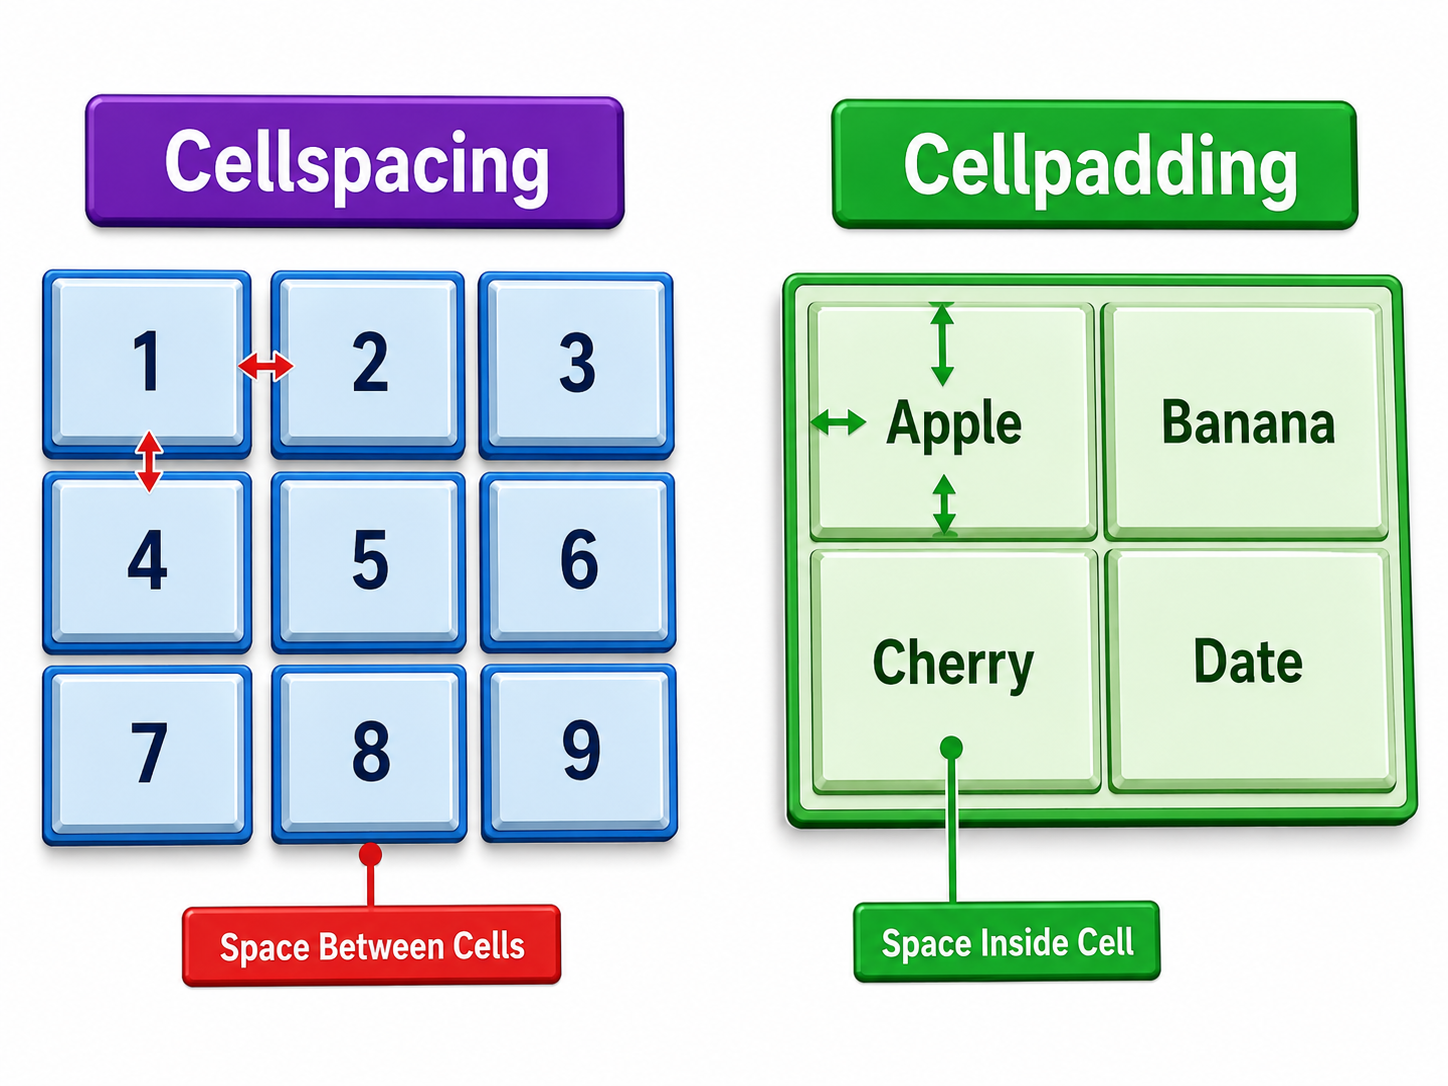
\includegraphics[width=0.95\linewidth,height=0.11\textheight,keepaspectratio]{chapters/Chapter04/topics/images/3d_cellspacing_vs_cellpadding.png}
}{
\fbox{\parbox{0.90\linewidth}{\centering\vspace{0.5cm}
\textbf{চিত্র}\\[4pt]
Left side: gap between two cell boxes labeled \texttt{cellspacing}. Right side: inner gap from content to cell wall labeled \texttt{cellpadding}.\\[4pt]
File: \texttt{chapters/Chapter04/topics/images/3d\_cellspacing\_vs\_cellpadding.png}
\vspace{0.5cm}}}
}
\captionof{figure}{cellspacing ও cellpadding-এর পার্থক্য}
\end{center}

\begin{keypointbox}{চিত্র ব্যাখ্যা}
চিত্রে \texttt{cellspacing} cell-এর মাঝের gap এবং \texttt{cellpadding} cell-এর ভিতরে content ও border-এর মাঝের gap তৈরি করে তা দেখানো হয়েছে।
\end{keypointbox}


\begin{keypointbox}{সহজ মনে রাখার উপায়}
Spacing মানে cell ও cell-এর মাঝে space। Padding মানে cell-এর ভিতরে content-এর চারপাশে space।
\end{keypointbox}

\subsection{\texttt{bgcolor} Attribute}

Table বা cell-এর background color দিতে \texttt{bgcolor} attribute ব্যবহার করা হয়।

\begin{examplebox}{কোড}
\begin{verbatim}
<!DOCTYPE html>
<html>
<head>
  <title>HTML Table Example</title>
</head>
<body>
<table border="1" bgcolor="yellow">
  <tr>
    <th>Name</th>
    <th>Class</th>
  </tr>
  <tr>
    <td>Rafi</td>
    <td>XI</td>
  </tr>
</table>
</body>
</html>
\end{verbatim}
\end{examplebox}

\subsection{\texttt{<td>} ও \texttt{<th>} Tag-এর Attribute}

Cell-এর উপর আলাদা control দেওয়ার জন্য \texttt{<td>} বা \texttt{<th>} tag-এর ভিতরে attribute ব্যবহার করা যায়।

PDF-এর table অংশে \texttt{<th>} ও \texttt{<td>} cell-এর জন্য আলাদা attribute দেখানো হয়েছে। একই table-এর সব cell একরকম নাও হতে পারে; কোনো cell center aligned, কোনো cell green background, কোনো cell বেশি wide, আবার কোনো cell একাধিক row বা column জুড়ে থাকতে পারে।

\begin{center}
\begin{tabular}{|p{0.18\textwidth}|p{0.46\textwidth}|p{0.25\textwidth}|}
\hline
\textbf{Attribute} & \textbf{কাজ} & \textbf{Example} \\
\hline
\texttt{align} & cell-এর text বাম/মাঝ/ডানে রাখে & \texttt{align="center"} \\
\hline
\texttt{valign} & cell-এর text top/middle/bottom রাখে & \texttt{valign="top"} \\
\hline
\texttt{bgcolor} & cell-এর background color দেয় & \texttt{bgcolor="green"} \\
\hline
\texttt{width} & cell-এর width নির্ধারণ করে & \texttt{width="150"} \\
\hline
\texttt{height} & cell-এর height নির্ধারণ করে & \texttt{height="60"} \\
\hline
\texttt{colspan} & cell-কে একাধিক column জুড়ে দেয় & \texttt{colspan="2"} \\
\hline
\texttt{rowspan} & cell-কে একাধিক row জুড়ে দেয় & \texttt{rowspan="3"} \\
\hline
\end{tabular}
\end{center}

\begin{keypointbox}{Color value}
\texttt{bgcolor} attribute-এ color name, hexadecimal value বা RGB ধরনের value ব্যবহার করা যায়। HSC practical-এ সাধারণত \texttt{yellow}, \texttt{green}, \texttt{silver} ধরনের color name বেশি দেখা যায়।
\end{keypointbox}

\subsection{\texttt{rowspan} ও \texttt{colspan}}

\begin{definitionbox}{\texttt{colspan}}
একটি cell-কে একাধিক column বা কলাম জুড়ে বিস্তৃত করার জন্য \texttt{colspan} attribute ব্যবহার করা হয়।
\end{definitionbox}

\begin{definitionbox}{\texttt{rowspan}}
একটি cell-কে একাধিক row বা সারি জুড়ে বিস্তৃত করার জন্য \texttt{rowspan} attribute ব্যবহার করা হয়।
\end{definitionbox}

\begin{examplebox}{\texttt{colspan} কোড}
\begin{verbatim}
<!DOCTYPE html>
<html>
<head>
  <title>HTML Table Example</title>
</head>
<body>
<table border="1">
  <tr>
    <th colspan="2">Student Info</th>
  </tr>
  <tr>
    <td>Roll</td>
    <td>101</td>
  </tr>
</table>
</body>
</html>
\end{verbatim}
\end{examplebox}

\begin{examplebox}{\texttt{rowspan} কোড}
\begin{verbatim}
<!DOCTYPE html>
<html>
<head>
  <title>HTML Table Example</title>
</head>
<body>
<table border="1">
  <tr>
    <th rowspan="2">Name</th>
    <td>Rafi</td>
  </tr>
  <tr>
    <td>Sakib</td>
  </tr>
</table>
</body>
</html>
\end{verbatim}
\end{examplebox}

\begin{center}
\IfFileExists{chapters/Chapter04/topics/images/3d_rowspan_colspan.png}{
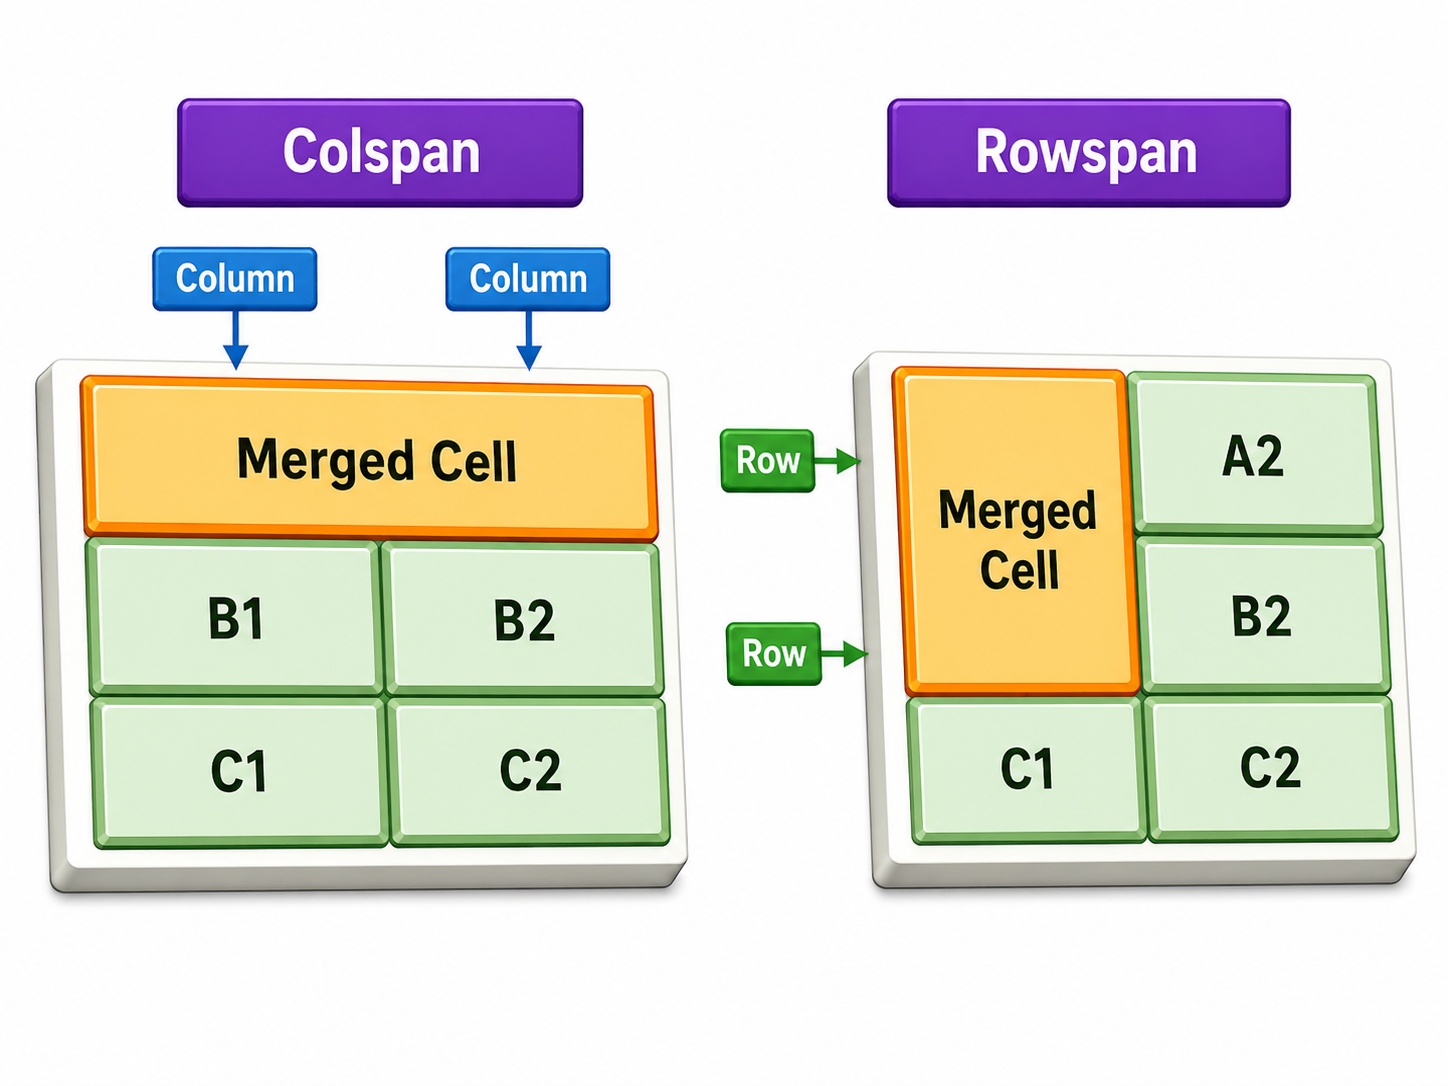
\includegraphics[width=0.95\linewidth,height=0.11\textheight,keepaspectratio]{chapters/Chapter04/topics/images/3d_rowspan_colspan.png}
}{
\fbox{\parbox{0.90\linewidth}{\centering\vspace{0.5cm}
\textbf{চিত্র}\\[4pt]
Two grids: one shows a wide block covering two columns labeled \texttt{colspan="2"}; another shows a tall block covering two rows labeled \texttt{rowspan="2"}.\\[4pt]
File: \texttt{chapters/Chapter04/topics/images/3d\_rowspan\_colspan.png}
\vspace{0.5cm}}}
}
\captionof{figure}{rowspan ও colspan দিয়ে cell merge}
\end{center}

\begin{keypointbox}{চিত্র ব্যাখ্যা}
চিত্রে \texttt{colspan} দিয়ে horizontal merge এবং \texttt{rowspan} দিয়ে vertical merge দেখানো হয়েছে। চিত্র দেখে code লেখার সময় merged cell আগে identify করতে হয়।
\end{keypointbox}


\begin{keypointbox}{Shortcut}
\texttt{colspan} = column span = পাশের দিকে merge।\\
\texttt{rowspan} = row span = নিচের দিকে merge।
\end{keypointbox}

\subsection{Merged Cell বুঝে Code লেখার নিয়ম}

Merged cell হলো এমন cell, যা একাধিক row বা column-এর জায়গা নেয়। Table চিত্র দেখে code লেখার সময় merged cell ভুল হলে পুরো table layout নষ্ট হয়ে যায়। তাই \texttt{rowspan} ও \texttt{colspan} ব্যবহার করার আগে base column সংখ্যা ঠিক করা দরকার।

\begin{boardbox}{\texttt{colspan} কখন ব্যবহার করবে}
যদি কোনো cell বাম থেকে ডানে একাধিক column-এর জায়গা নেয়, তখন \texttt{colspan} ব্যবহার করবে। যেমন, একটি title যদি table-এর তিনটি column জুড়ে থাকে, তাহলে code হবে \texttt{<th colspan="3">Title</th>}।
\end{boardbox}

\begin{boardbox}{\texttt{rowspan} কখন ব্যবহার করবে}
যদি কোনো cell উপর থেকে নিচে একাধিক row-এর জায়গা নেয়, তখন \texttt{rowspan} ব্যবহার করবে। যেমন, একটি group name যদি দুইটি section row-এর জন্য common হয়, তাহলে code হবে \texttt{<td rowspan="2">Science</td>}।
\end{boardbox}

\begin{keypointbox}{Merged cell-এর কারণে cell count কমে যায়}
যে row-তে \texttt{colspan} বা \texttt{rowspan} ব্যবহার করা হয়, সেই row-তে আলাদা cell কম লিখতে হয়। কারণ merged cell নিজেই একাধিক cell-এর জায়গা দখল করে। এটাই beginners-দের সবচেয়ে সাধারণ ভুল।
\end{keypointbox}

\subsection{Empty Cell এবং \texttt{\&nbsp;}}

Table-এর কোনো cell খালি রাখতে চাইলে অনেক সময় browser cell-এর border ঠিকভাবে দেখাতে সমস্যা করতে পারে। তাই খালি cell-এ non-breaking space বা \texttt{\&nbsp;} ব্যবহার করা হয়।

খালি cell রাখা দরকার হলে শুধু blank space না দিয়ে \texttt{\&nbsp;} লেখা ভালো, কারণ এটি একটি invisible character হিসেবে কাজ করে। ফলে cell-এর height, width এবং border ঠিক থাকে। Board practical-এ empty cell দেখলে \texttt{<td>\&nbsp;</td>} লিখলে layout বেশি নির্ভরযোগ্য হয়। পুরনো বইয়ের example-এ খালি cell দেখাতে অনেক সময় \texttt{<br>} ব্যবহারও দেখা যায়, তবে পরীক্ষায় পরিষ্কারভাবে empty cell বোঝাতে \texttt{\&nbsp;} বেশি নির্ভরযোগ্য।

\begin{examplebox}{কোড}
\begin{verbatim}
<!DOCTYPE html>
<html>
<head>
  <title>Empty Cell Example</title>
</head>
<body>
  <table border="1" cellspacing="0" cellpadding="6">
    <tr>
      <th>Header 1</th>
      <th>Header 2</th>
    </tr>
    <tr>
      <td>Data</td>
      <td>&nbsp;</td>
    </tr>
  </table>
</body>
</html>
\end{verbatim}
\end{examplebox}

\conceptwrapimage{chapters/Chapter04/topics/images/3d_empty_cell_nbsp.png}
{চিত্রে empty cell দৃশ্যমান রাখতে \texttt{\&nbsp;} ব্যবহারের ধারণা দেখানো হয়েছে। খালি cell collapse বা অস্পষ্ট হলে non-breaking space ব্যবহার করা যায়।}
{খালি cell-এ \texttt{\&nbsp;} ব্যবহার}


\subsection{\texttt{<caption>} Tag}

\begin{definitionbox}{\texttt{<caption>} tag}
HTML table-এর শিরোনাম বা title প্রদর্শনের জন্য \texttt{<caption>} tag ব্যবহার করা হয়।
\end{definitionbox}

\texttt{<caption>} tag সবসময় \texttt{<table>} tag-এর ভিতরে এবং প্রথম row-এর আগে লেখা উচিত। এতে browser সাধারণত table-এর উপরে title দেখায়। Result sheet, routine, admission list বা product table-এর মতো table-এ caption দিলে table-এর উদ্দেশ্য দ্রুত বোঝা যায়। পুরনো HSC-style code-এ caption-এর position বোঝাতে \texttt{align="bottom"} ধরনের legacy attribute দেখা যেতে পারে, তবে modern HTML-এ caption position CSS দিয়ে নিয়ন্ত্রণ করা ভালো।

\begin{examplebox}{কোড}
\begin{verbatim}
<!DOCTYPE html>
<html>
<head>
  <title>Caption Example</title>
</head>
<body>
  <table border="1" cellspacing="0" cellpadding="6">
    <caption>Student Information</caption>
    <tr>
      <th>Roll</th>
      <th>Name</th>
      <th>Result</th>
    </tr>
    <tr>
      <td>101</td>
      <td>Sakib</td>
      <td>A+</td>
    </tr>
  </table>
</body>
</html>
\end{verbatim}
\end{examplebox}

\conceptwrapimage{chapters/Chapter04/topics/images/3d_caption.png}
{চিত্রে table-এর উপরে caption/title দেখানো হয়েছে। HTML-এ \texttt{<caption>} tag table-এর title লিখতে ব্যবহৃত হয়।}
{table caption}


\subsection{\texttt{colgroup} Tag}

\begin{definitionbox}{\texttt{<colgroup>} tag}
Table-এর এক বা একাধিক column-এর জন্য একসাথে style বা property নির্ধারণ করতে \texttt{<colgroup>} tag ব্যবহার করা হয়।
\end{definitionbox}

\texttt{colgroup} ব্যবহার করলে কোনো নির্দিষ্ট column বা column group-কে আলাদা color/style দেওয়া যায়। এটি table-এর row শুরু হওয়ার আগে লেখা হয়, কারণ column style আগে ঠিক করে তারপর row data বসানো হয়।

একই ধরনের একাধিক column একসাথে style করতে \texttt{<col span="2">} ব্যবহার করা যায়। যেমন প্রথম দুই column এক color এবং পরের দুই column আরেক color করতে চাইলে \texttt{span} attribute helpful। প্রতিটি column আলাদা style চাইলে আলাদা আলাদা \texttt{<col>} tag লেখা হয়।

\begin{examplebox}{কোড}
\begin{verbatim}
<!DOCTYPE html>
<html>
<head>
  <title>Column Group Example</title>
</head>
<body>
<table border="1">
  <colgroup>
    <col style="background-color: yellow">
    <col style="background-color: lightgreen">
  </colgroup>
  <tr>
    <th>Title</th>
    <th>Author</th>
  </tr>
  <tr>
    <td>ICT HSC</td>
    <td>M. Hakim</td>
  </tr>
</table>
</body>
</html>
\end{verbatim}
\end{examplebox}

\conceptwrapimage{chapters/Chapter04/topics/images/3d_colgroup.png}
{চিত্রে \texttt{<colgroup>} ব্যবহার করে নির্দিষ্ট column group-এ style দেওয়ার ধারণা দেখানো হয়েছে। এতে একাধিক column একসাথে color/style করা যায়।}
{colgroup দিয়ে column style}


\subsection{Table-এর ভিতরে Formatting, Link, Image ও List}

Table cell-এর ভিতরে শুধু text নয়, HTML-এর অন্য element-ও রাখা যায়। PDF-এর table discussion-এ cell-এর ভিতরে text, image, photograph, list, form, horizontal line, hyperlink এবং আরেকটি table রাখার ধারণা আছে। তাই table ব্যবহার করে result sheet-এর সাথে photo, product list-এর সাথে buy link, course plan-এর সাথে ordered list বা nested information দেখানো সম্ভব।

\begin{keypointbox}{Cell-এর ভিতরে content রাখার নিয়ম}
Cell-এর ভিতরে content রাখতে হলে content অবশ্যই \texttt{<td>} বা \texttt{<th>} tag-এর opening ও closing tag-এর মাঝখানে লিখতে হবে। যেমন image বসাতে \texttt{<td><img src="photo.jpg"></td>} এবং link বসাতে \texttt{<td><a href="page.html">Open</a></td>} লিখতে হবে।
\end{keypointbox}

\begin{center}
\begin{tabular}{|p{0.22\textwidth}|p{0.50\textwidth}|p{0.18\textwidth}|}
\hline
\textbf{Content type} & \textbf{Cell-এর ভিতরে code idea} & \textbf{Tag} \\
\hline
Text & \texttt{<td>Rafi</td>} & \texttt{<td>} \\
\hline
Image & \texttt{<td><img src="a.jpg"></td>} & \texttt{<img>} \\
\hline
Link & \texttt{<td><a href="a.html">Open</a></td>} & \texttt{<a>} \\
\hline
List & \texttt{<td><ol>...</ol></td>} & \texttt{<ol>}, \texttt{<li>} \\
\hline
Horizontal line & \texttt{<td><hr></td>} & \texttt{<hr>} \\
\hline
Form control & \texttt{<td><input type="text"></td>} & \texttt{<input>} \\
\hline
Nested table & \texttt{<td><table>...</table></td>} & \texttt{<table>} \\
\hline
\end{tabular}
\end{center}

\subsubsection{Formatting Text}

\begin{examplebox}{কোড}
\begin{verbatim}
<!DOCTYPE html>
<html>
<head>
  <title>Cell Formatting Example</title>
</head>
<body>
  <table border="1" cellspacing="0" cellpadding="6">
    <tr>
      <td><b>ICT</b></td>
      <td><u>HSC</u></td>
      <td><i>Book</i></td>
    </tr>
  </table>
</body>
</html>
\end{verbatim}
\end{examplebox}

\subsubsection{Hyperlink}

\begin{examplebox}{কোড}
\begin{verbatim}
<!DOCTYPE html>
<html>
<head>
  <title>Table Link Example</title>
</head>
<body>
  <table border="1" cellspacing="0" cellpadding="6">
    <tr>
      <td>
        <a href="https://www.educationboard.gov.bd">Education Board</a>
      </td>
    </tr>
  </table>
</body>
</html>
\end{verbatim}
\end{examplebox}

\subsubsection{Image}

\begin{examplebox}{কোড}
\begin{verbatim}
<!DOCTYPE html>
<html>
<head>
  <title>Table Image Example</title>
</head>
<body>
  <table border="1" cellspacing="0" cellpadding="6">
    <tr>
      <td>
        <img src="photo.jpg" width="100" height="80" alt="Photo">
      </td>
    </tr>
  </table>
</body>
</html>
\end{verbatim}
\end{examplebox}

\subsubsection{List}

\begin{center}
\IfFileExists{chapters/Chapter04/topics/images/3d_content_inside_cell.png}{
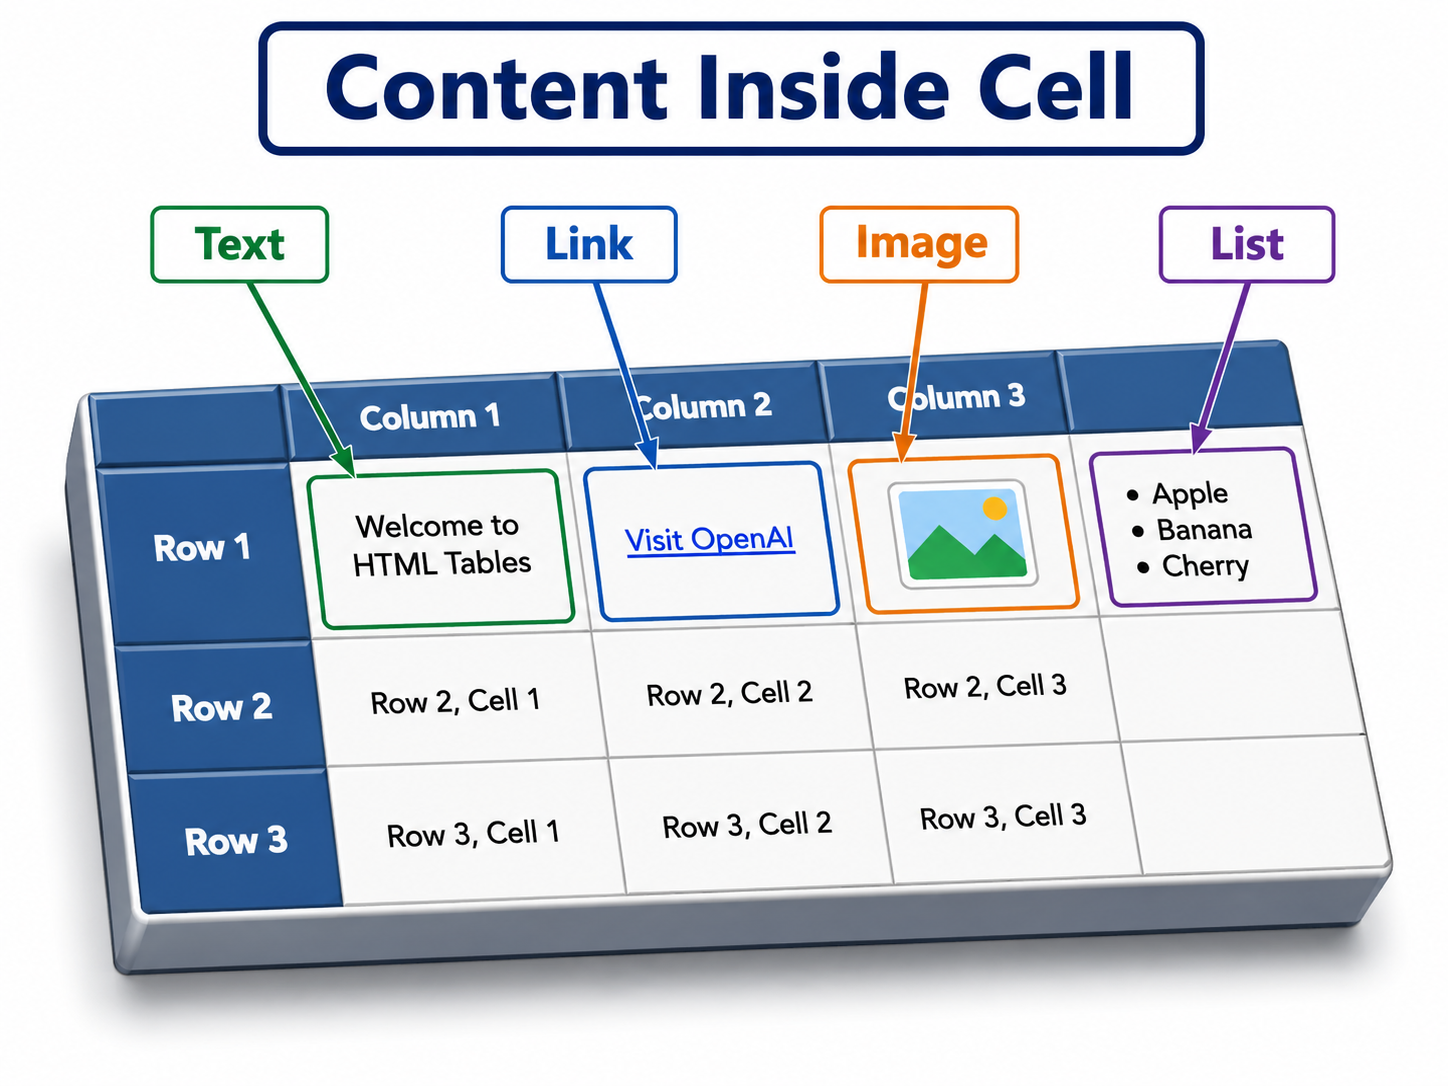
\includegraphics[width=0.78\linewidth,height=0.12\textheight,keepaspectratio]{chapters/Chapter04/topics/images/3d_content_inside_cell.png}
}{
\fbox{\parbox{0.90\linewidth}{\centering\vspace{0.35cm}
\textbf{চিত্র}\\[3pt]
File: \texttt{chapters/Chapter04/topics/images/3d\_content\_inside\_cell.png}
\vspace{0.35cm}}}
}
\captionof{figure}{table cell-এর ভিতরে text, link, image ও list}
\end{center}

\noindent{\color{blue!62!black}\bfseries চিত্র ব্যাখ্যা:}
চিত্রে table cell-এর ভিতরে চার ধরনের content দেখানো হয়েছে: normal text, hyperlink, image এবং ordered list। List cell-এর ভিতরে \texttt{<ol>} ও \texttt{<li>} tag ব্যবহার করা হয়েছে।

\begin{keypointbox}{চিত্র দেখে code লেখার ধাপ}
যে cell-এর ভিতরে list থাকবে, সেখানে প্রথমে \texttt{<td>} লিখবে। তারপর cell-এর ভিতরে \texttt{<ol>} বা \texttt{<ul>} tag লিখে প্রতিটি item \texttt{<li>} দিয়ে লিখবে।
\end{keypointbox}

\begin{examplebox}{কোড}
\begin{verbatim}
<!DOCTYPE html>
<html>
<head>
  <title>List Inside Table Example</title>
</head>
<body>
  <table border="1" cellspacing="0" cellpadding="6">
    <tr>
      <td>
        <ol>
          <li>Dhaka</li>
          <li>Dinajpur</li>
          <li>Rangpur</li>
        </ol>
      </td>
    </tr>
  </table>
</body>
</html>
\end{verbatim}
\end{examplebox}

\subsection{Nested Table বা Table-এর ভিতরে Table}

\begin{definitionbox}{Nested Table}
একটি table-এর কোনো cell-এর ভিতরে আরেকটি table তৈরি করলে তাকে nested table বলা হয়।
\end{definitionbox}

\begin{examplebox}{কোড}
\begin{verbatim}
<!DOCTYPE html>
<html>
<head>
  <title>Nested Table Example</title>
</head>
<body>
  <table border="1" cellspacing="0" cellpadding="10">
    <tr>
      <td>Parent Cell</td>
      <td>
        <table border="1" cellspacing="0" cellpadding="5">
          <tr>
            <th>Child</th>
            <th>Table</th>
          </tr>
          <tr>
            <td>A</td>
            <td>B</td>
          </tr>
        </table>
      </td>
    </tr>
  </table>
</body>
</html>
\end{verbatim}
\end{examplebox}

\conceptwrapimage{chapters/Chapter04/topics/images/3d_nested_table.png}
{চিত্রে parent table-এর একটি cell-এর ভিতরে child table বসানো হয়েছে। এটিকে nested table বা table inside table বলা হয়।}
{table-এর ভিতরে nested table}

\begin{keypointbox}{Nested table লেখার সতর্কতা}
Nested table লিখলে outer table ও inner table-এর tag আলাদা করে close করতে হবে। প্রথমে inner table-এর \texttt{</table>} close করবে, তারপর outer cell-এর \texttt{</td>} এবং শেষে outer table close করবে। ভুল জায়গায় \texttt{</table>} দিলে output ভেঙে যায়।
\end{keypointbox}


\subsection{Modern CSS Note}

\begin{keypointbox}{Modern note}
HSC ICT basic HTML অংশে \texttt{border}, \texttt{align}, \texttt{bgcolor}, \texttt{cellpadding}, \texttt{cellspacing}, \texttt{width} attribute শেখা দরকার। তবে professional web design-এ এগুলোর অনেকগুলো কাজ CSS দিয়ে করা হয়। যেমন: \texttt{border}, \texttt{border-collapse}, \texttt{border-spacing}, \texttt{padding}, \texttt{text-align}, \texttt{background-color}, \texttt{width}।
\end{keypointbox}

\begin{examplebox}{Modern CSS Version}
\begin{verbatim}
<!DOCTYPE html>
<html>
<head>
  <title>Modern Table</title>
  <style>
    table {
      width: 400px;
      border-collapse: collapse;
    }
    th, td {
      border: 1px solid black;
      padding: 8px;
      text-align: center;
    }
    th {
      background-color: lightgray;
    }
  </style>
</head>
<body>
  <table>
    <tr>
      <th>Roll</th>
      <th>Name</th>
    </tr>
    <tr>
      <td>101</td>
      <td>Rafi</td>
    </tr>
  </table>
</body>
</html>
\end{verbatim}
\end{examplebox}

\subsection{Semantic ও Readability Note}

HSC book-style code-এ \texttt{border}, \texttt{cellpadding}, \texttt{cellspacing}, \texttt{align}, \texttt{bgcolor} attribute দেখা যায়। এগুলো practical exam-এর জন্য জানা দরকার। তবে modern HTML-এ table-এর visual style সাধারণত CSS দিয়ে করা হয়। Table-এর meaning পরিষ্কার রাখতে heading cell-এ \texttt{<th>} ব্যবহার করা উচিত এবং table-এর title থাকলে \texttt{<caption>} ব্যবহার করা উচিত।

\begin{boardbox}{ভালো table code-এর বৈশিষ্ট্য}
\begin{itemize}
\item Table data row-column আকারে logical হবে।
\item Heading cell-এ \texttt{<th>} ব্যবহার করা হবে।
\item Caption থাকলে \texttt{<caption>} table-এর শুরুতে লেখা হবে।
\item Image থাকলে \texttt{alt} attribute ব্যবহার করা হবে।
\item Link থাকলে meaningful text ব্যবহার করা হবে।
\item Tag indentation পরিষ্কার হলে code পড়া সহজ হবে।
\end{itemize}
\end{boardbox}

\subsection{চিত্র দেখে Table Code লেখার ধাপ}

HSC exam-এ চিত্র দেখে table code লিখতে হলে আগে table-টি বিশ্লেষণ করতে হবে।

\begin{enumerate}
\item মোট কয়টি row আছে দেখো।
\item সর্বোচ্চ কয়টি column আছে দেখো।
\item heading cell আছে কি না দেখো।
\item কোনো cell merge আছে কি না দেখো।
\item cell merge হলে সেটি \texttt{rowspan} নাকি \texttt{colspan} তা নির্ধারণ করো।
\item border, width, align, cellspacing, cellpadding দরকার কি না দেখো।
\item image, link, list বা nested table আছে কি না দেখো।
\item তারপর \texttt{<table>} skeleton লিখে row অনুযায়ী cell বসাও।
\end{enumerate}

\begin{center}
\IfFileExists{chapters/Chapter04/topics/images/3d_figure_to_code_steps.png}{
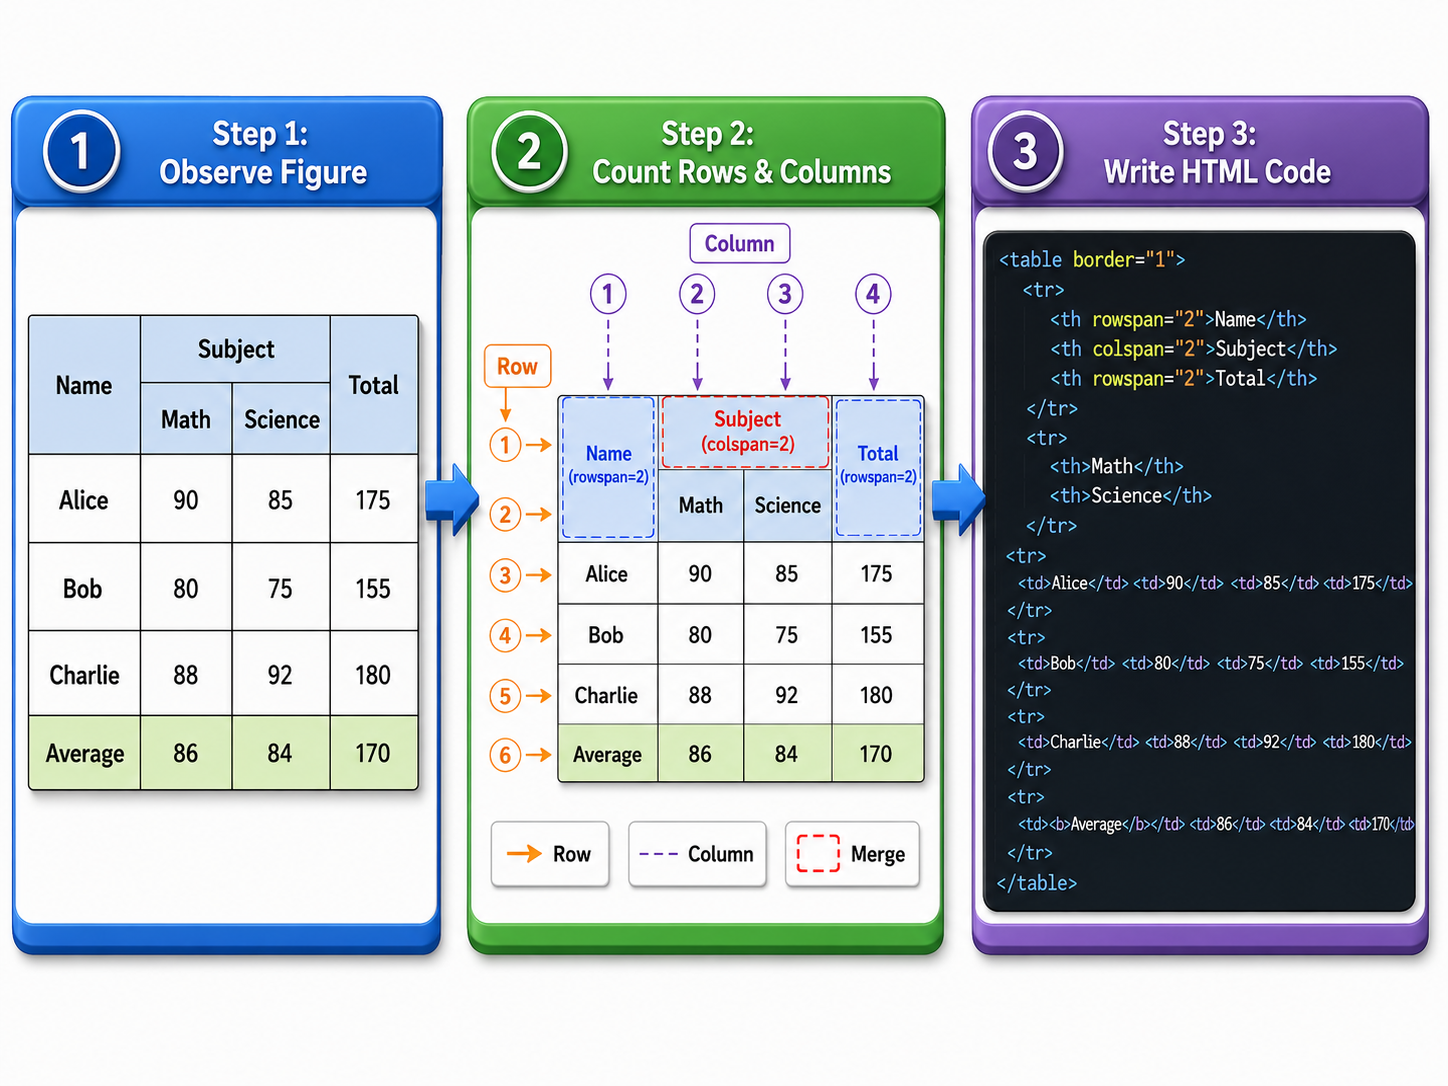
\includegraphics[width=0.95\linewidth,height=0.11\textheight,keepaspectratio]{chapters/Chapter04/topics/images/3d_figure_to_code_steps.png}
}{
\fbox{\parbox{0.90\linewidth}{\centering\vspace{0.5cm}
\textbf{চিত্র}\\[4pt]
A flow diagram: count rows $\rightarrow$ count columns $\rightarrow$ find merged cells $\rightarrow$ add content $\rightarrow$ write HTML code.\\[4pt]
File: \texttt{chapters/Chapter04/topics/images/3d\_figure\_to\_code\_steps.png}
\vspace{0.5cm}}}
}
\captionof{figure}{figure থেকে HTML table code লেখার ধাপ}
\end{center}

\begin{keypointbox}{চিত্র ব্যাখ্যা}
চিত্রে চিত্র দেখে HTML table code লেখার workflow দেখানো হয়েছে: row-column count করা, merged cell identify করা, content type বোঝা এবং শেষে HTML tag লেখা।
\end{keypointbox}


\subsection{PDF Exercise Bank: First to Last}

এই অংশে PDF-এর page অনুযায়ী table exercise সাজানো হয়েছে। প্রত্যেক exercise-এ concept, চিত্র, চিত্র ব্যাখ্যা, code লেখার ধাপ এবং কোড দেওয়া হয়েছে।

\begin{multicols}{2}
\raggedcolumns
\setlength{\columnsep}{10pt}
\subsubsection{Exercise 1: Basic Row and Column Table}

\begin{boardbox}{Concept}
প্রথম table exercise-এ 2 row এবং 2 column দিয়ে basic cell structure বোঝানো হয়েছে।
\end{boardbox}

\begin{center}
\IfFileExists{chapters/Chapter04/topics/images/ex01_3d_basic_2x2.png}{
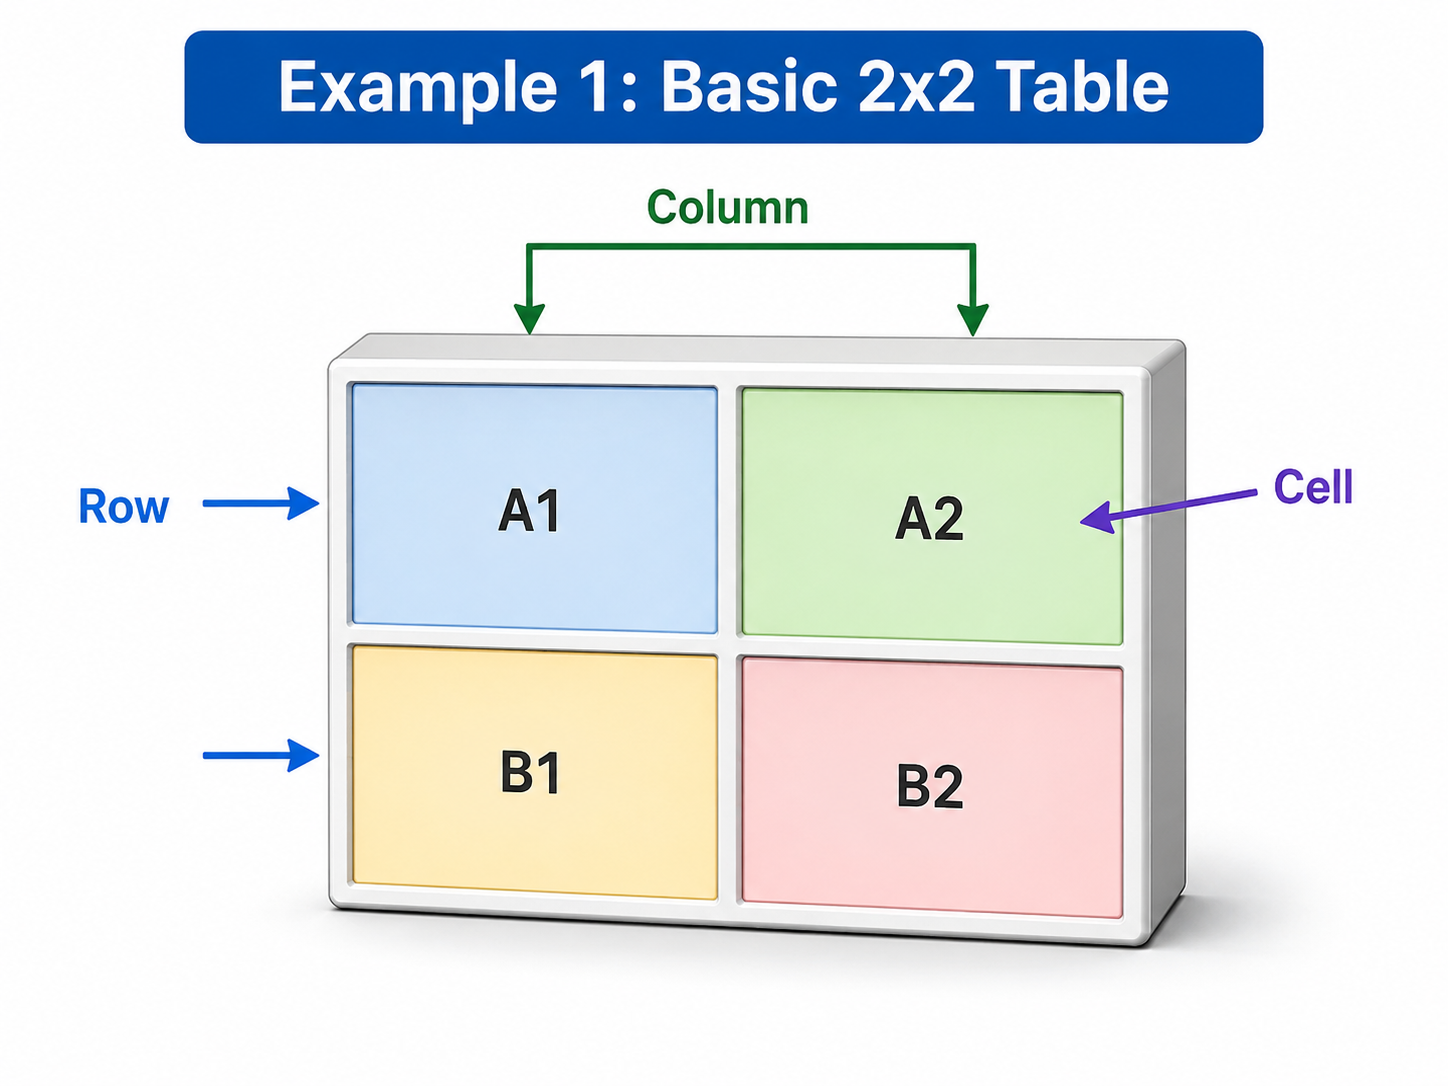
\includegraphics[width=0.95\linewidth,height=0.11\textheight,keepaspectratio]{chapters/Chapter04/topics/images/ex01_3d_basic_2x2.png}
}{
\fbox{\parbox{0.90\linewidth}{\centering\vspace{0.4cm}
\textbf{চিত্র}\\
File: \texttt{chapters/Chapter04/topics/images/ex01\_3d\_basic\_2x2.png}
\vspace{0.4cm}}}
}
\captionof{figure}{Exercise 1-এর table চিত্র}
\end{center}

\begin{keypointbox}{চিত্র ব্যাখ্যা}
চিত্রে A1, A2, B1 এবং B2 নামে চারটি cell আছে। প্রথম row-তে A1-A2 এবং দ্বিতীয় row-তে B1-B2 রাখা হয়েছে।
\end{keypointbox}

\begin{keypointbox}{চিত্র দেখে code লেখার ধাপ}
প্রথমে 2টি row ধরবে। প্রতিটি row-তে 2টি করে \texttt{<td>} cell লিখবে। তারপর cell text হিসেবে A1, A2, B1, B2 বসাবে।
\end{keypointbox}

\par\noindent{\color{purple!70!black}\bfseries\small কোড}\par\vspace{-4pt}
\begin{verbatim}
<!DOCTYPE html>
<html>
<head>
  <title>HTML Table Example</title>
</head>
<body>
<table>
  <tr>
    <td>A1</td>
    <td>A2</td>
  </tr>
  <tr>
    <td>B1</td>
    <td>B2</td>
  </tr>
</table>
</body>
</html>
\end{verbatim}
\vspace{-6pt}

\subsubsection{Exercise 2: Border সহ Simple Table}

\begin{boardbox}{Concept}
\texttt{border="1"} দিলে table এবং cell-এর চারপাশে border দেখা যায়।
\end{boardbox}

\begin{center}
\IfFileExists{chapters/Chapter04/topics/images/ex02_3d_border_table.png}{
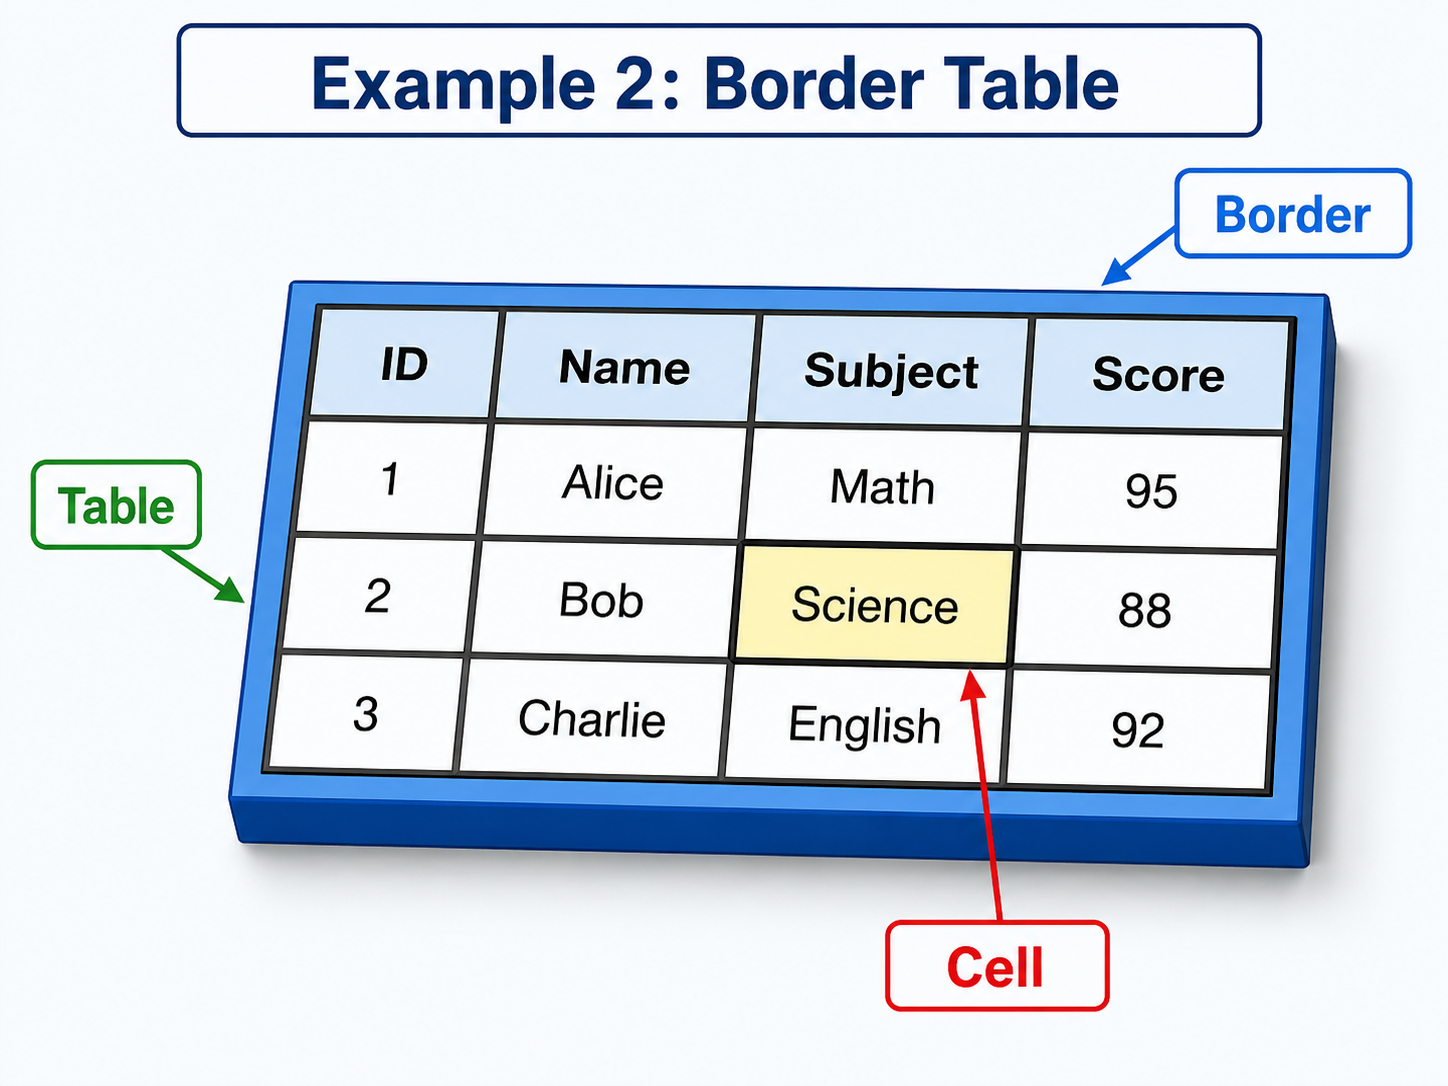
\includegraphics[width=0.95\linewidth,height=0.11\textheight,keepaspectratio]{chapters/Chapter04/topics/images/ex02_3d_border_table.png}
}{
\fbox{\parbox{0.90\linewidth}{\centering\vspace{0.4cm}
\textbf{চিত্র}\\
File: \texttt{chapters/Chapter04/topics/images/ex02\_3d\_border\_table.png}
\vspace{0.4cm}}}
}
\captionof{figure}{Exercise 2-এর border চিত্র}
\end{center}

\begin{keypointbox}{চিত্র ব্যাখ্যা}
চিত্রে ID, Name, Subject এবং Score column আছে। তিনজন student-এর subject ও score border সহ table আকারে দেখানো হয়েছে।
\end{keypointbox}

\begin{keypointbox}{চিত্র দেখে code লেখার ধাপ}
প্রথমে header row-তে চারটি \texttt{<th>} লিখবে। এরপর Alice, Bob ও Charlie-এর জন্য তিনটি data row তৈরি করবে। পুরো table-এ border দেখাতে \texttt{border="1"} ব্যবহার করবে।
\end{keypointbox}

\par\noindent{\color{purple!70!black}\bfseries\small কোড}\par\vspace{-4pt}
\begin{verbatim}
<!DOCTYPE html>
<html>
<head>
  <title>HTML Table Example</title>
</head>
<body>
<table border="1" cellspacing="0" cellpadding="6">
  <tr>
    <th>ID</th>
    <th>Name</th>
    <th>Subject</th>
    <th>Score</th>
  </tr>
  <tr>
    <td>1</td>
    <td>Alice</td>
    <td>Math</td>
    <td>95</td>
  </tr>
  <tr>
    <td>2</td>
    <td>Bob</td>
    <td>Science</td>
    <td>88</td>
  </tr>
  <tr>
    <td>3</td>
    <td>Charlie</td>
    <td>English</td>
    <td>92</td>
  </tr>
</table>
</body>
</html>
\end{verbatim}
\vspace{-6pt}

\subsubsection{Exercise 3: Caption, TH এবং Student Info Table}

\begin{boardbox}{Concept}
\texttt{<caption>} table-এর title দেয় এবং \texttt{<th>} heading cell তৈরি করে।
\end{boardbox}

\begin{center}
\IfFileExists{chapters/Chapter04/topics/images/ex03_3d_student_info.png}{
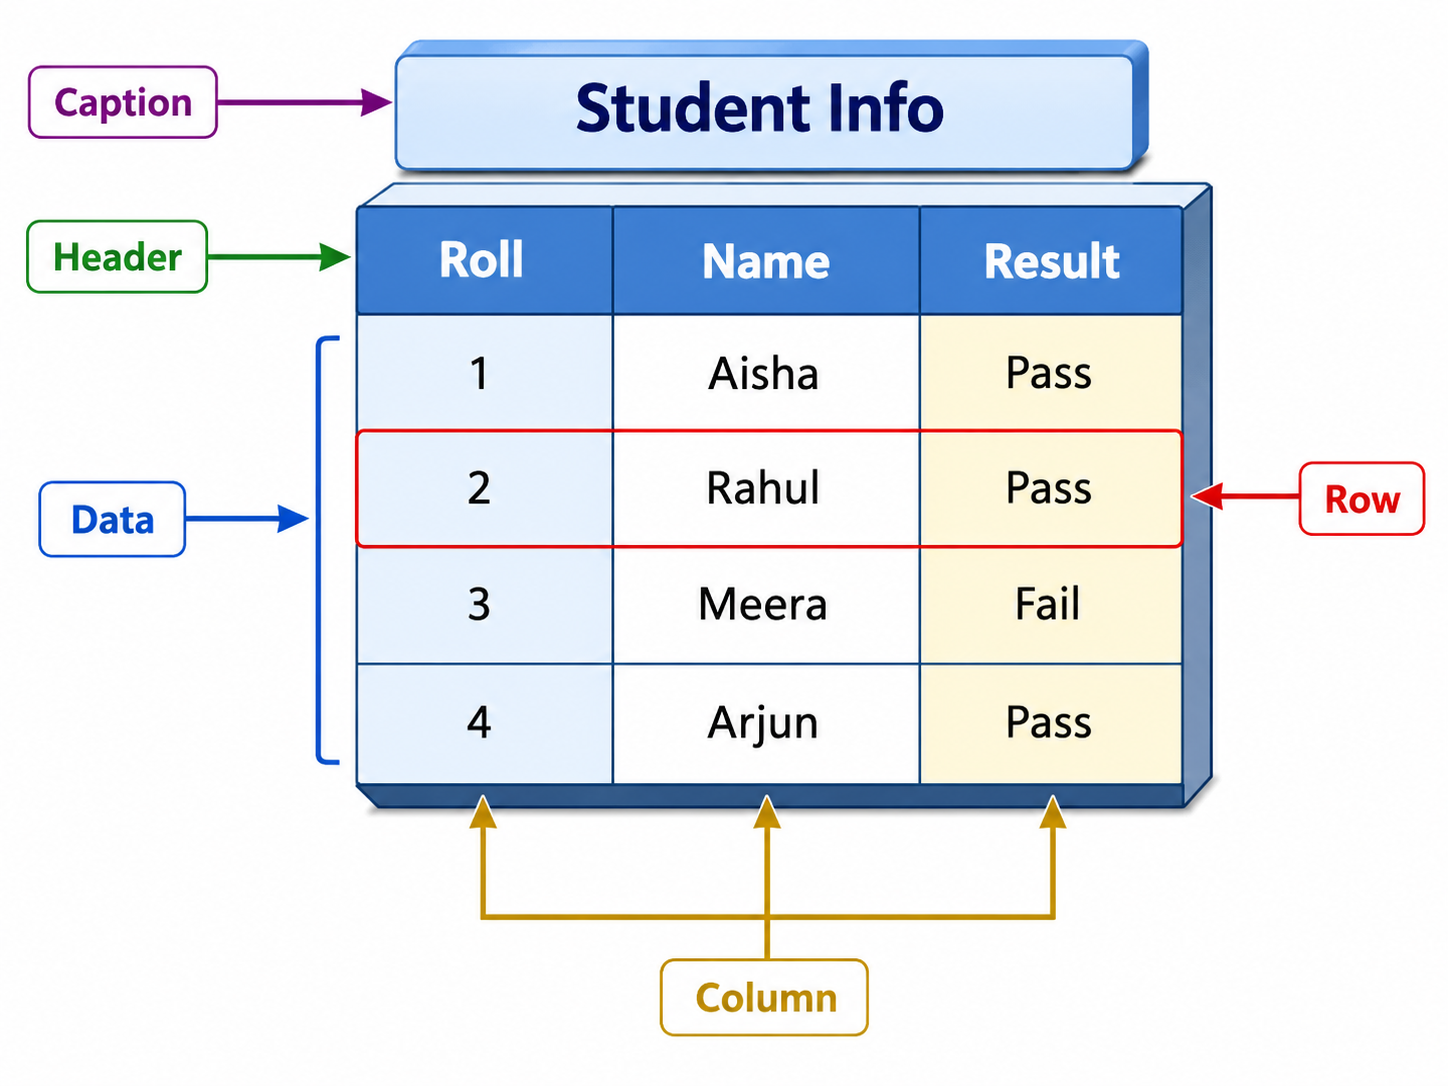
\includegraphics[width=0.95\linewidth,height=0.11\textheight,keepaspectratio]{chapters/Chapter04/topics/images/ex03_3d_student_info.png}
}{
\fbox{\parbox{0.90\linewidth}{\centering\vspace{0.4cm}
\textbf{চিত্র}\\
File: \texttt{chapters/Chapter04/topics/images/ex03\_3d\_student\_info.png}
\vspace{0.4cm}}}
}
\captionof{figure}{Exercise 3-এর caption ও heading চিত্র}
\end{center}

\begin{keypointbox}{চিত্র ব্যাখ্যা}
চিত্রে Student Info caption আছে। table-এ Roll, Name ও Result column দেখানো হয়েছে এবং data row-গুলোতে Pass/Fail result আছে।
\end{keypointbox}

\begin{keypointbox}{চিত্র দেখে code লেখার ধাপ}
প্রথমে \texttt{<caption>} দিয়ে Student Info লিখবে। এরপর তিনটি header cell তৈরি করবে। তারপর চারটি student row লিখবে।
\end{keypointbox}

\par\noindent{\color{purple!70!black}\bfseries\small কোড}\par\vspace{-4pt}
\begin{verbatim}
<!DOCTYPE html>
<html>
<head>
  <title>HTML Table Example</title>
</head>
<body>
<table border="1" cellspacing="0" cellpadding="6">
  <caption><b>Student Info</b></caption>
  <tr>
    <th>Roll</th>
    <th>Name</th>
    <th>Result</th>
  </tr>
  <tr><td>1</td><td>Aisha</td><td>Pass</td></tr>
  <tr><td>2</td><td>Rahul</td><td>Pass</td></tr>
  <tr><td>3</td><td>Meera</td><td>Fail</td></tr>
  <tr><td>4</td><td>Arjun</td><td>Pass</td></tr>
</table>
</body>
</html>
\end{verbatim}
\vspace{-6pt}

\subsubsection{Exercise 4: Width Attribute দিয়ে Table Width নির্ধারণ}

\begin{boardbox}{Concept}
\texttt{width} attribute দিয়ে table-এর মোট প্রস্থ নির্ধারণ করা যায়।
\end{boardbox}

\begin{center}
\IfFileExists{chapters/Chapter04/topics/images/ex04_3d_width_400.png}{
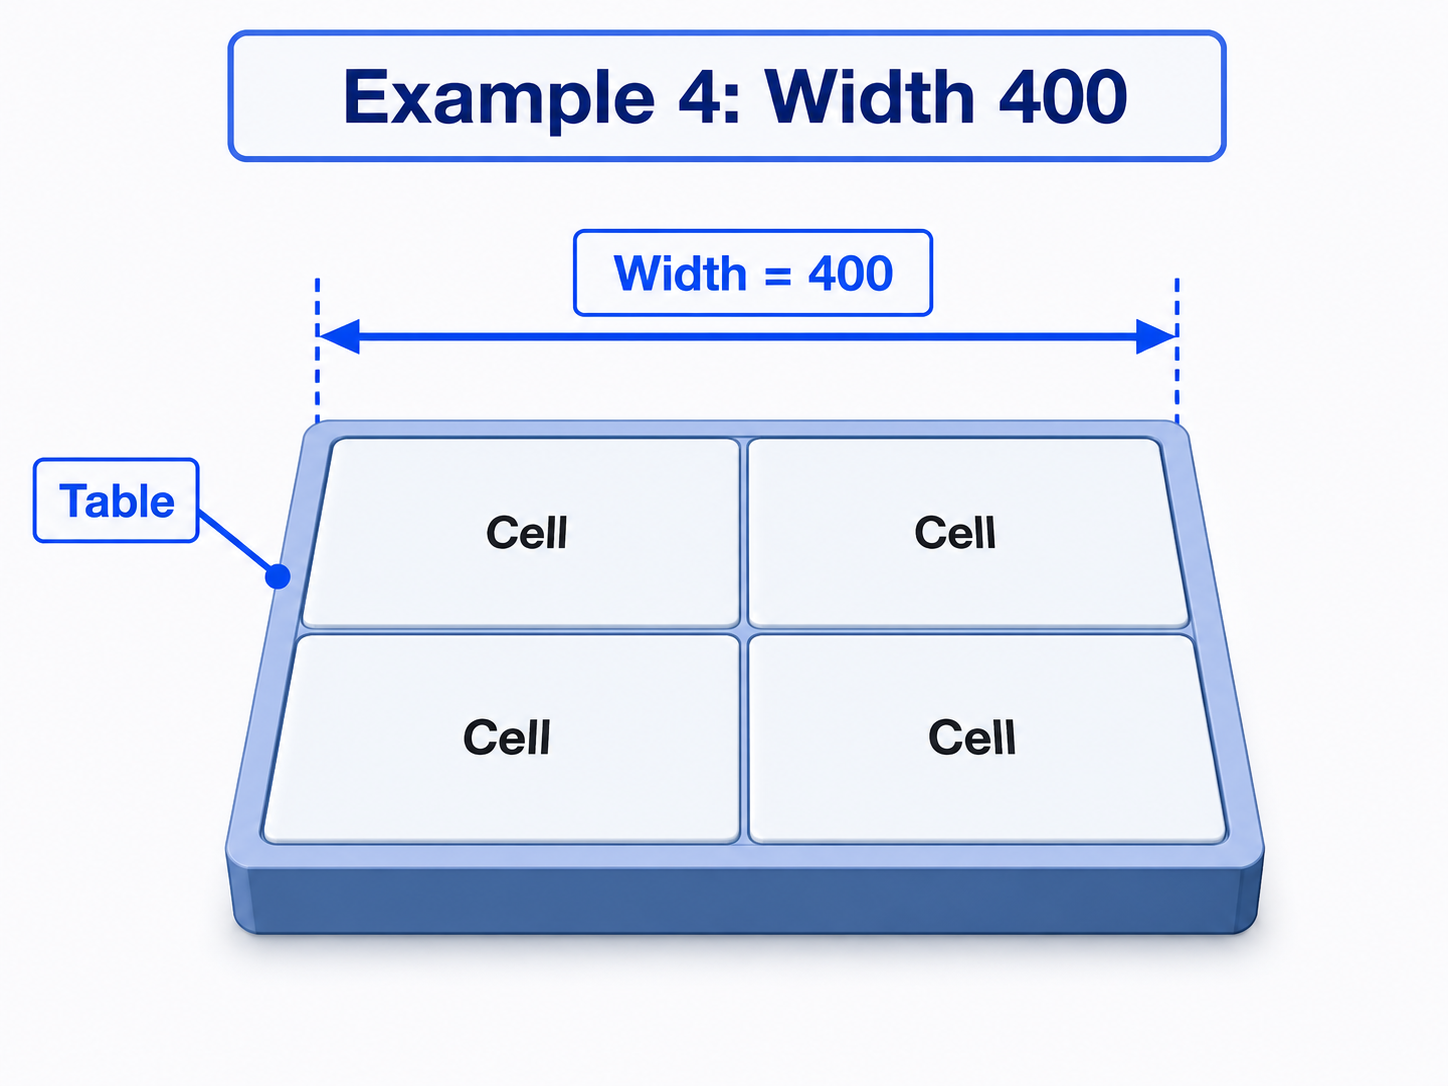
\includegraphics[width=0.95\linewidth,height=0.11\textheight,keepaspectratio]{chapters/Chapter04/topics/images/ex04_3d_width_400.png}
}{
\fbox{\parbox{0.90\linewidth}{\centering\vspace{0.4cm}
\textbf{চিত্র}\\
File: \texttt{chapters/Chapter04/topics/images/ex04\_3d\_width\_400.png}
\vspace{0.4cm}}}
}
\captionof{figure}{Exercise 4-এর width চিত্র}
\end{center}

\begin{keypointbox}{চিত্র ব্যাখ্যা}
চিত্রে table width 400 দেখানো হয়েছে। table-টি 2 row ও 2 column-এর, প্রতিটি cell-এ Cell লেখা আছে।
\end{keypointbox}

\begin{keypointbox}{চিত্র দেখে code লেখার ধাপ}
প্রথমে \texttt{width="400"} সহ table লিখবে। তারপর 2টি row এবং প্রতিটি row-তে 2টি cell তৈরি করবে।
\end{keypointbox}

\par\noindent{\color{purple!70!black}\bfseries\small কোড}\par\vspace{-4pt}
\begin{verbatim}
<!DOCTYPE html>
<html>
<head>
  <title>HTML Table Example</title>
</head>
<body>
<table border="1" width="400" cellspacing="0" cellpadding="10">
  <tr>
    <td>Cell</td>
    <td>Cell</td>
  </tr>
  <tr>
    <td>Cell</td>
    <td>Cell</td>
  </tr>
</table>
</body>
</html>
\end{verbatim}
\vspace{-6pt}

\subsubsection{Exercise 5: Table Attribute Practice}

\begin{boardbox}{Concept}
একই table-এ \texttt{border}, \texttt{width}, \texttt{cellspacing}, \texttt{cellpadding}, \texttt{align} ও \texttt{bgcolor} attribute ব্যবহার করা যায়।
\end{boardbox}

\begin{center}
\IfFileExists{chapters/Chapter04/topics/images/ex05_3d_table_attributes_combined.png}{
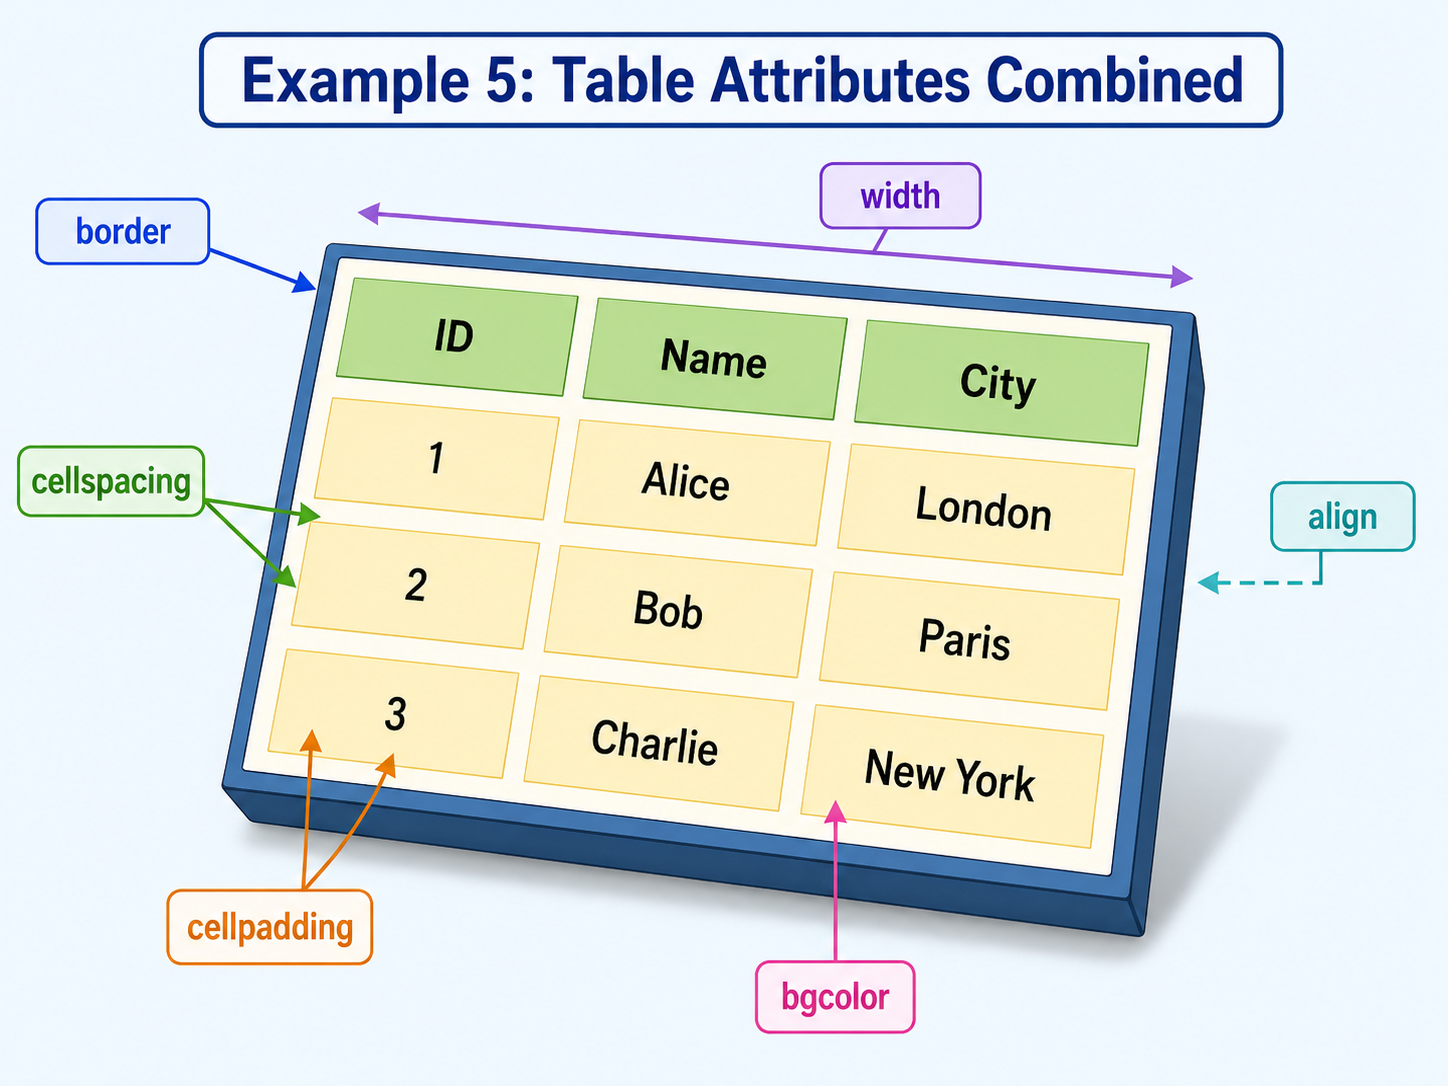
\includegraphics[width=0.95\linewidth,height=0.11\textheight,keepaspectratio]{chapters/Chapter04/topics/images/ex05_3d_table_attributes_combined.png}
}{
\fbox{\parbox{0.90\linewidth}{\centering\vspace{0.4cm}
\textbf{চিত্র}\\
File: \texttt{chapters/Chapter04/topics/images/ex05\_3d\_table\_attributes\_combined.png}
\vspace{0.4cm}}}
}
\captionof{figure}{Exercise 5-এর attribute চিত্র}
\end{center}

\begin{keypointbox}{চিত্র ব্যাখ্যা}
চিত্রে একটি student/city table-এর উপর table attributes-এর effect দেখানো হয়েছে। header background color, table width, border, spacing, padding এবং alignment visual label দিয়ে বোঝানো হয়েছে।
\end{keypointbox}

\begin{keypointbox}{চিত্র দেখে code লেখার ধাপ}
প্রথমে table tag-এ attribute বসাবে। তারপর ID, Name, City header row লিখবে। শেষে তিনটি data row তৈরি করবে।
\end{keypointbox}

\par\noindent{\color{purple!70!black}\bfseries\small কোড}\par\vspace{-4pt}
\begin{verbatim}
<!DOCTYPE html>
<html>
<head>
  <title>HTML Table Example</title>
</head>
<body>
<table border="1" width="450" cellspacing="6" cellpadding="8" align="center">
  <tr bgcolor="lightgreen">
    <th>ID</th>
    <th>Name</th>
    <th>City</th>
  </tr>
  <tr><td>1</td><td>Alice</td><td>London</td></tr>
  <tr><td>2</td><td>Bob</td><td>Paris</td></tr>
  <tr><td>3</td><td>Charlie</td><td>New York</td></tr>
</table>
</body>
</html>
\end{verbatim}
\vspace{-6pt}

\subsubsection{Exercise 6: Colspan ও Rowspan Basic Example}

\begin{boardbox}{Concept}
\texttt{colspan} horizontal cell merge করে এবং \texttt{rowspan} vertical cell merge করে।
\end{boardbox}

\begin{center}
\IfFileExists{chapters/Chapter04/topics/images/ex06_3d_span_two_columns_rows.png}{
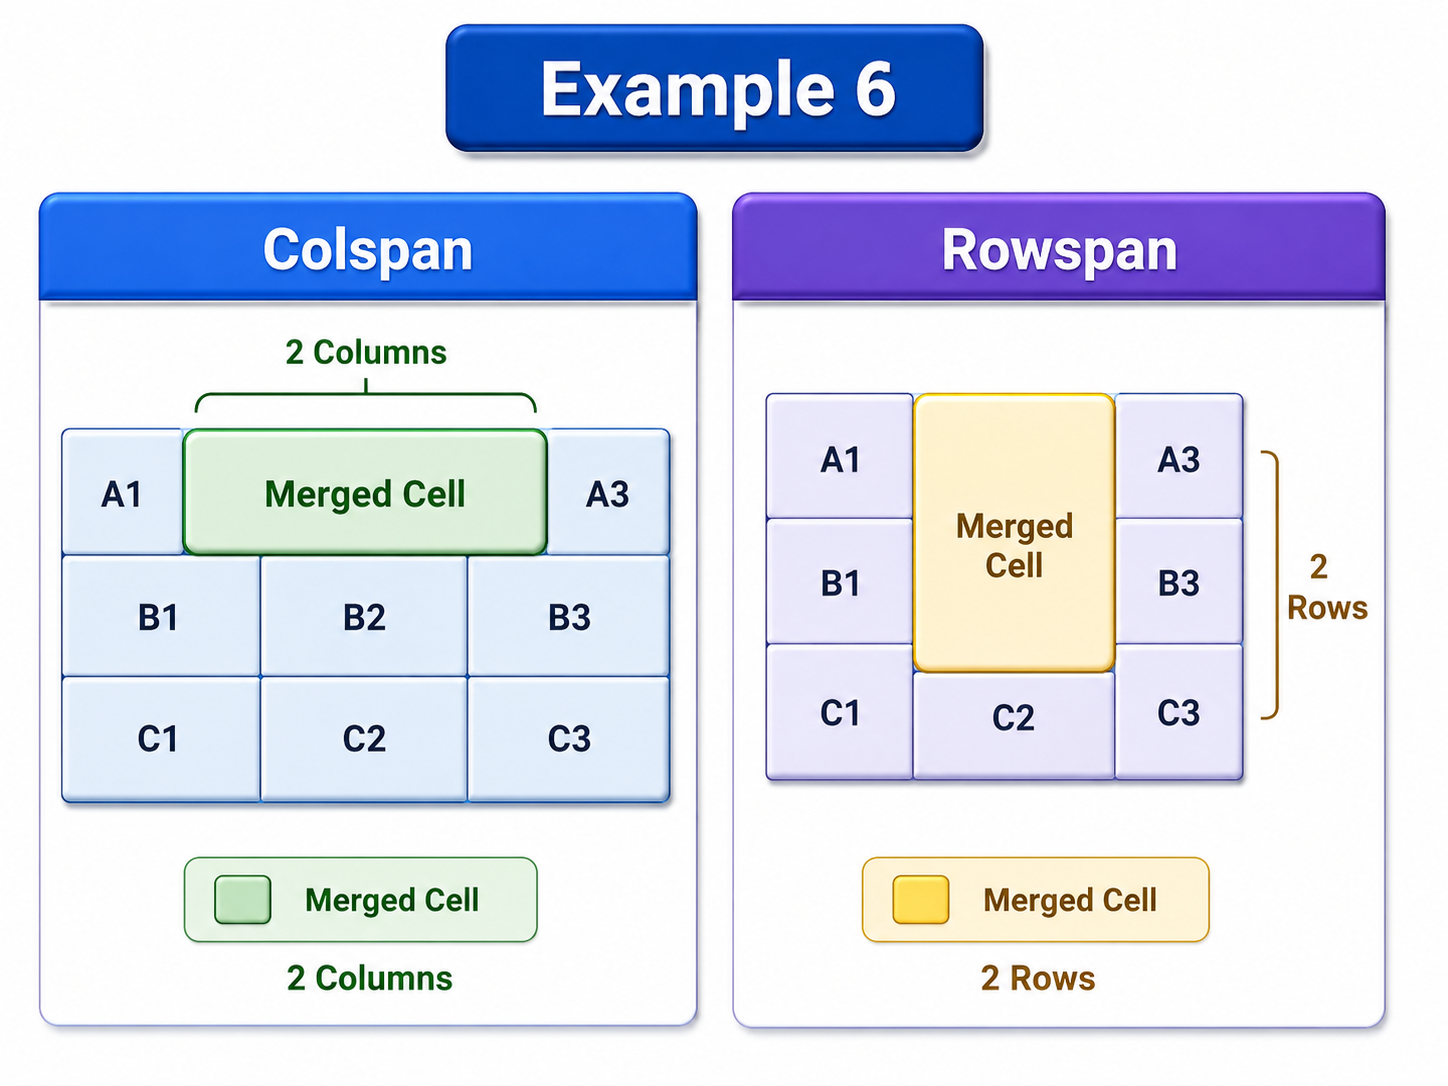
\includegraphics[width=0.95\linewidth,height=0.11\textheight,keepaspectratio]{chapters/Chapter04/topics/images/ex06_3d_span_two_columns_rows.png}
}{
\fbox{\parbox{0.90\linewidth}{\centering\vspace{0.4cm}
\textbf{চিত্র}\\
File: \texttt{chapters/Chapter04/topics/images/ex06\_3d\_span\_two\_columns\_rows.png}
\vspace{0.4cm}}}
}
\captionof{figure}{Exercise 6-এর rowspan-colspan চিত্র}
\end{center}

\begin{keypointbox}{চিত্র ব্যাখ্যা}
চিত্রে বাম পাশে colspan দিয়ে দুই column merge এবং ডান পাশে rowspan দিয়ে দুই row merge দেখানো হয়েছে।
\end{keypointbox}

\begin{keypointbox}{চিত্র দেখে code লেখার ধাপ}
Horizontal merge দরকার হলে \texttt{colspan="2"} ব্যবহার করবে। Vertical merge দরকার হলে \texttt{rowspan="2"} ব্যবহার করবে।
\end{keypointbox}

\par\noindent{\color{purple!70!black}\bfseries\small কোড}\par\vspace{-4pt}
\begin{verbatim}
<!DOCTYPE html>
<html>
<head>
  <title>HTML Table Example</title>
</head>
<body>
<h3>Colspan</h3>
<table border="1" cellspacing="0" cellpadding="6">
  <tr><th colspan="3">Colspan</th></tr>
  <tr><td>A1</td><td colspan="2">Merged Cell</td></tr>
  <tr><td>B1</td><td>B2</td><td>B3</td></tr>
  <tr><td>C1</td><td>C2</td><td>C3</td></tr>
</table>

<h3>Rowspan</h3>
<table border="1" cellspacing="0" cellpadding="6">
  <tr><th colspan="3">Rowspan</th></tr>
  <tr><td>A1</td><td rowspan="2">Merged Cell</td><td>A3</td></tr>
  <tr><td>B1</td><td>B3</td></tr>
  <tr><td>C1</td><td>C2</td><td>C3</td></tr>
</table>
</body>
</html>
\end{verbatim}
\vspace{-6pt}

\subsubsection{Exercise 7: Empty Cell এবং Basic Sales Table}

\begin{boardbox}{Concept}
খালি cell দেখাতে cell-এর ভিতরে \texttt{\&nbsp;} ব্যবহার করা যায়।
\end{boardbox}

\begin{center}
\IfFileExists{chapters/Chapter04/topics/images/ex07_3d_empty_cells.png}{
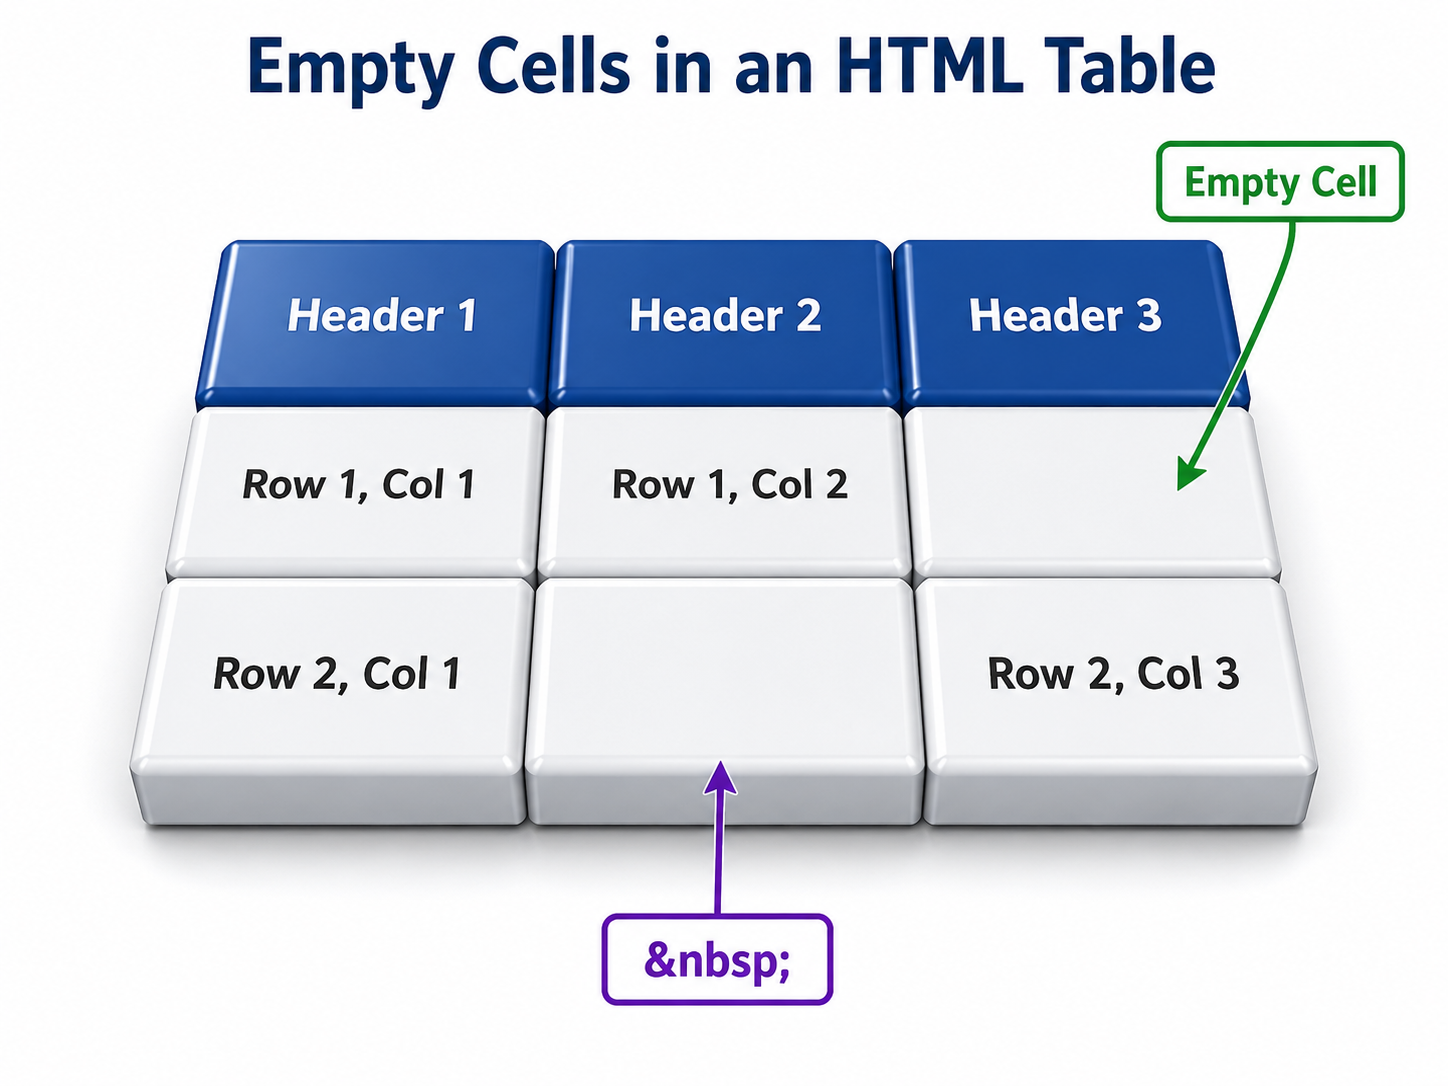
\includegraphics[width=0.95\linewidth,height=0.11\textheight,keepaspectratio]{chapters/Chapter04/topics/images/ex07_3d_empty_cells.png}
}{
\fbox{\parbox{0.90\linewidth}{\centering\vspace{0.4cm}
\textbf{চিত্র}\\
File: \texttt{chapters/Chapter04/topics/images/ex07\_3d\_empty\_cells.png}
\vspace{0.4cm}}}
}
\captionof{figure}{Exercise 7-এর empty cell চিত্র}
\end{center}

\begin{keypointbox}{চিত্র ব্যাখ্যা}
চিত্রে Header 1, Header 2, Header 3 সহ table আছে। কিছু cell intentionally empty রাখা হয়েছে; browser-এ cell visible রাখতে \texttt{\&nbsp;} ব্যবহার করা হয়েছে।
\end{keypointbox}

\begin{keypointbox}{চিত্র দেখে code লেখার ধাপ}
প্রথমে তিনটি header লিখবে। যে cell খালি দেখাতে হবে সেখানে normal text না দিয়ে \texttt{\&nbsp;} লিখবে।
\end{keypointbox}

\par\noindent{\color{purple!70!black}\bfseries\small কোড}\par\vspace{-4pt}
\begin{verbatim}
<!DOCTYPE html>
<html>
<head>
  <title>HTML Table Example</title>
</head>
<body>
<table border="1" cellspacing="0" cellpadding="8">
  <tr>
    <th>Header 1</th>
    <th>Header 2</th>
    <th>Header 3</th>
  </tr>
  <tr>
    <td>Row 1, Col 1</td>
    <td>Row 1, Col 2</td>
    <td>&nbsp;</td>
  </tr>
  <tr>
    <td>Row 2, Col 1</td>
    <td>&nbsp;</td>
    <td>Row 2, Col 3</td>
  </tr>
</table>
</body>
</html>
\end{verbatim}
\vspace{-6pt}

\subsubsection{Exercise 8: Align Attribute Practice}

\begin{boardbox}{Concept}
\texttt{align="center"} দিলে cell-এর content horizontally center হয়।
\end{boardbox}

\begin{center}
\IfFileExists{chapters/Chapter04/topics/images/ex08_3d_align_center.png}{
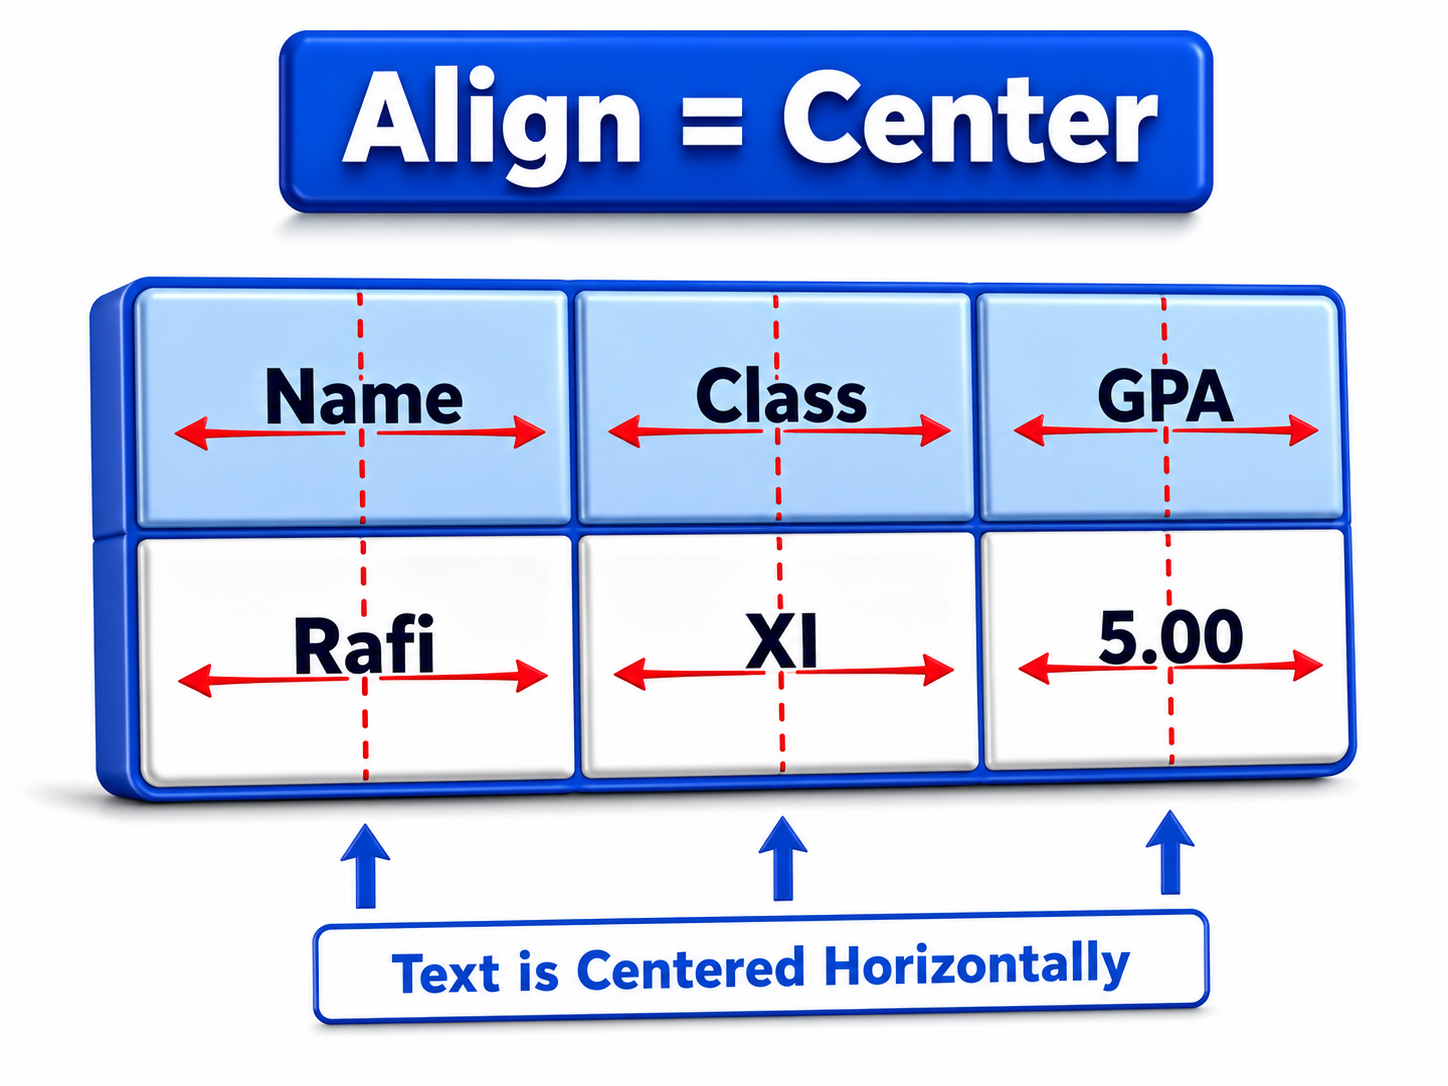
\includegraphics[width=0.95\linewidth,height=0.11\textheight,keepaspectratio]{chapters/Chapter04/topics/images/ex08_3d_align_center.png}
}{
\fbox{\parbox{0.90\linewidth}{\centering\vspace{0.4cm}
\textbf{চিত্র}\\
File: \texttt{chapters/Chapter04/topics/images/ex08\_3d\_align\_center.png}
\vspace{0.4cm}}}
}
\captionof{figure}{Exercise 8-এর align চিত্র}
\end{center}

\begin{keypointbox}{চিত্র ব্যাখ্যা}
চিত্রে Name, Class ও GPA column-এর text center aligned আছে। Rafi, XI এবং 5.00 cell-গুলো cell-এর মাঝখানে বসেছে।
\end{keypointbox}

\begin{keypointbox}{চিত্র দেখে code লেখার ধাপ}
পুরো table center alignment করতে table row বা প্রতিটি cell-এ \texttt{align="center"} ব্যবহার করবে।
\end{keypointbox}

\par\noindent{\color{purple!70!black}\bfseries\small কোড}\par\vspace{-4pt}
\begin{verbatim}
<!DOCTYPE html>
<html>
<head>
  <title>HTML Table Example</title>
</head>
<body>
<table border="1" cellspacing="0" cellpadding="8" align="center">
  <tr align="center">
    <th>Name</th>
    <th>Class</th>
    <th>GPA</th>
  </tr>
  <tr align="center">
    <td>Rafi</td>
    <td>XI</td>
    <td>5.00</td>
  </tr>
</table>
</body>
</html>
\end{verbatim}
\vspace{-6pt}

\subsubsection{Exercise 9: Cell Data Alignment Table}

\begin{boardbox}{Concept}
একই table-এ left, center এবং right alignment আলাদা cell-এ ব্যবহার করা যায়।
\end{boardbox}

\begin{center}
\IfFileExists{chapters/Chapter04/topics/images/ex09_3d_cell_alignment.png}{
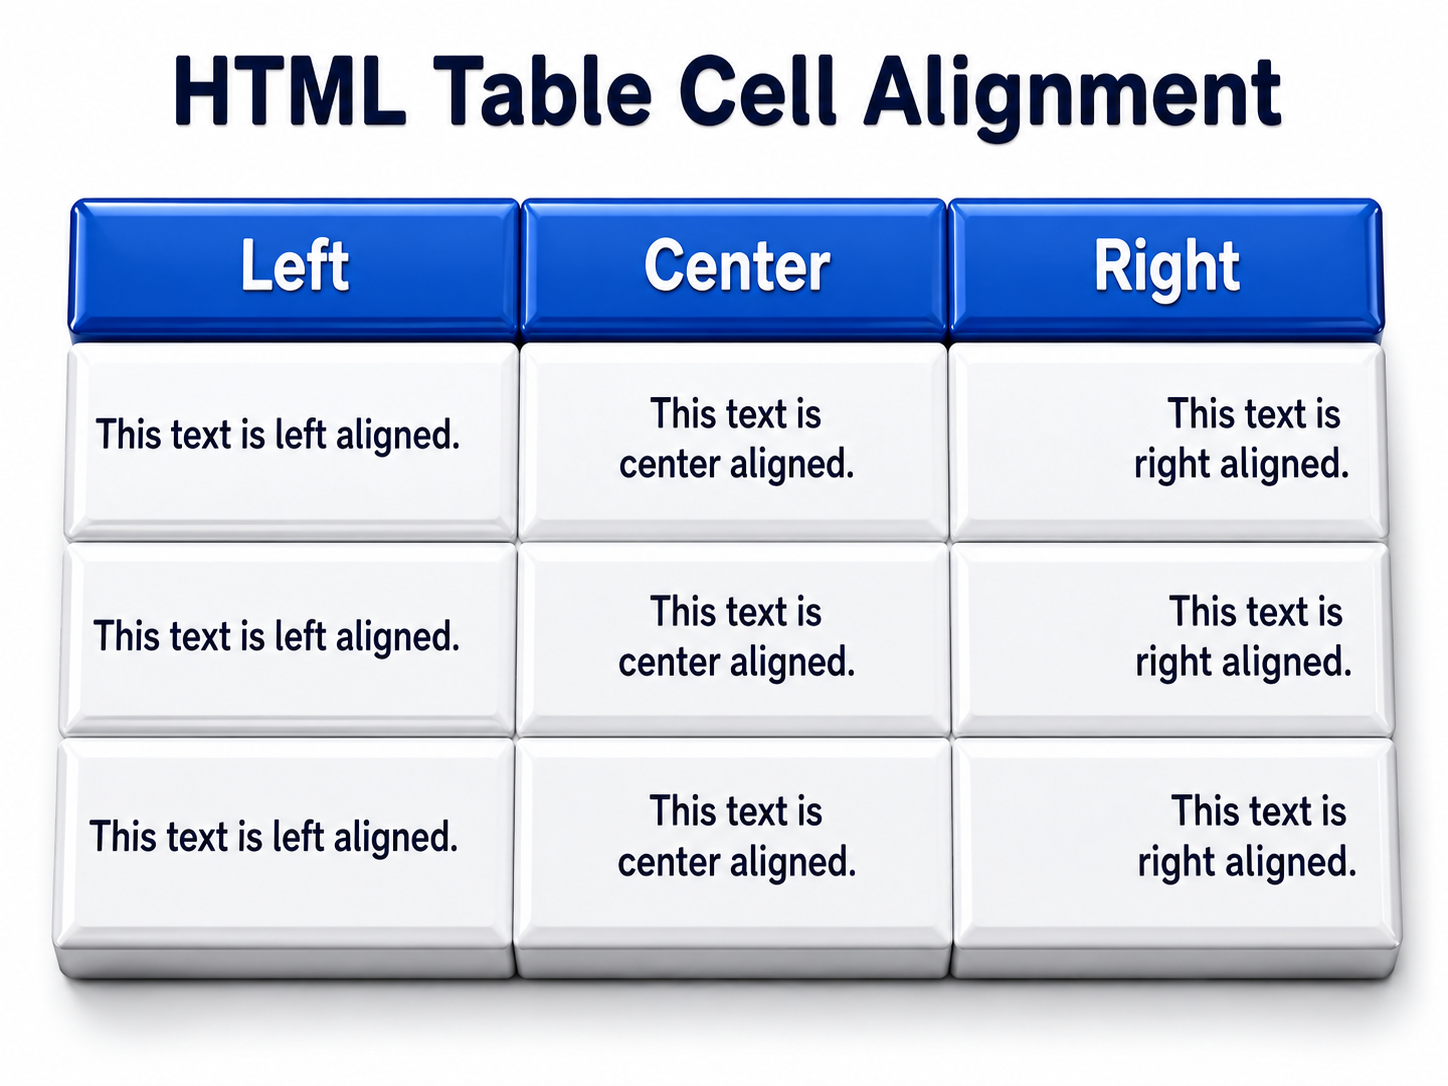
\includegraphics[width=0.95\linewidth,height=0.11\textheight,keepaspectratio]{chapters/Chapter04/topics/images/ex09_3d_cell_alignment.png}
}{
\fbox{\parbox{0.90\linewidth}{\centering\vspace{0.4cm}
\textbf{চিত্র}\\
File: \texttt{chapters/Chapter04/topics/images/ex09\_3d\_cell\_alignment.png}
\vspace{0.4cm}}}
}
\captionof{figure}{Exercise 9-এর cell alignment চিত্র}
\end{center}

\begin{keypointbox}{চিত্র ব্যাখ্যা}
চিত্রে তিনটি column আছে: Left, Center, Right। প্রতিটি column-এর text নিজ নিজ alignment অনুযায়ী cell-এর বাম, মাঝ বা ডান পাশে বসেছে।
\end{keypointbox}

\begin{keypointbox}{চিত্র দেখে code লেখার ধাপ}
Left column-এর cell-এ \texttt{align="left"}, center column-এ \texttt{align="center"} এবং right column-এ \texttt{align="right"} ব্যবহার করবে।
\end{keypointbox}

\par\noindent{\color{purple!70!black}\bfseries\small কোড}\par\vspace{-4pt}
\begin{verbatim}
<!DOCTYPE html>
<html>
<head>
  <title>HTML Table Example</title>
</head>
<body>
<table border="1" cellspacing="0" cellpadding="8">
  <tr>
    <th>Left</th>
    <th>Center</th>
    <th>Right</th>
  </tr>
  <tr>
    <td align="left">This text is left aligned.</td>
    <td align="center">This text is center aligned.</td>
    <td align="right">This text is right aligned.</td>
  </tr>
  <tr>
    <td align="left">This text is left aligned.</td>
    <td align="center">This text is center aligned.</td>
    <td align="right">This text is right aligned.</td>
  </tr>
</table>
</body>
</html>
\end{verbatim}
\vspace{-6pt}

\subsubsection{Exercise 10: Cell Width/Height Change}

\begin{boardbox}{Concept}
\texttt{width} ও \texttt{height} attribute দিয়ে cell-এর size change করা যায়।
\end{boardbox}

\begin{center}
\IfFileExists{chapters/Chapter04/topics/images/ex10_3d_cell_width_height.png}{
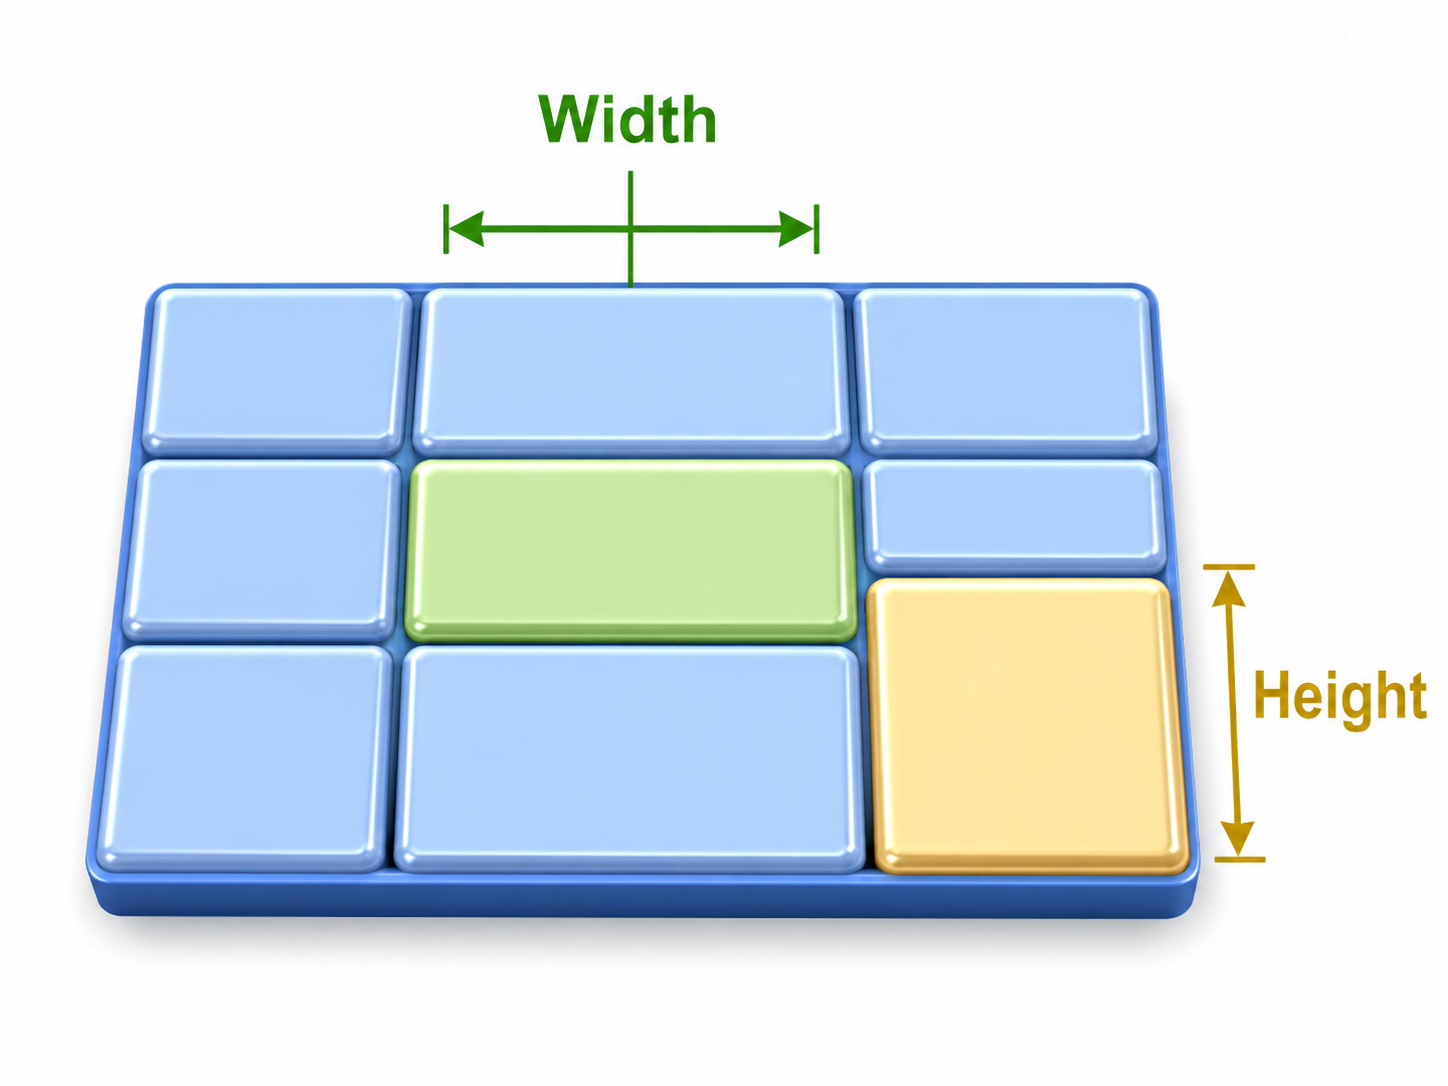
\includegraphics[width=0.95\linewidth,height=0.11\textheight,keepaspectratio]{chapters/Chapter04/topics/images/ex10_3d_cell_width_height.png}
}{
\fbox{\parbox{0.90\linewidth}{\centering\vspace{0.4cm}
\textbf{চিত্র}\\
File: \texttt{chapters/Chapter04/topics/images/ex10\_3d\_cell\_width\_height.png}
\vspace{0.4cm}}}
}
\captionof{figure}{Exercise 10-এর width-height চিত্র}
\end{center}

\begin{keypointbox}{চিত্র ব্যাখ্যা}
চিত্রে একটি table-এর মাঝের cell-এ width বেশি এবং ডান দিকের নিচের cell-এ height বেশি দেখানো হয়েছে।
\end{keypointbox}

\begin{keypointbox}{চিত্র দেখে code লেখার ধাপ}
যে cell চওড়া হবে সেখানে \texttt{width} attribute এবং যে cell লম্বা হবে সেখানে \texttt{height} attribute বসাবে।
\end{keypointbox}

\par\noindent{\color{purple!70!black}\bfseries\small কোড}\par\vspace{-4pt}
\begin{verbatim}
<!DOCTYPE html>
<html>
<head>
  <title>HTML Table Example</title>
</head>
<body>
<table border="1" cellspacing="0" cellpadding="8">
  <tr><td>A1</td><td>A2</td><td>A3</td></tr>
  <tr><td>B1</td><td width="120">Wide Cell</td><td>B3</td></tr>
  <tr><td>C1</td><td>C2</td><td height="80">Tall Cell</td></tr>
</table>
</body>
</html>
\end{verbatim}
\vspace{-6pt}

\subsubsection{Exercise 11: Month Income Cost Table}

\begin{boardbox}{Concept}
\texttt{valign} attribute দিয়ে cell-এর content vertically top, middle বা bottom position-এ রাখা যায়।
\end{boardbox}

\begin{center}
\IfFileExists{chapters/Chapter04/topics/images/ex11_3d_valign_month_income_cost.png}{
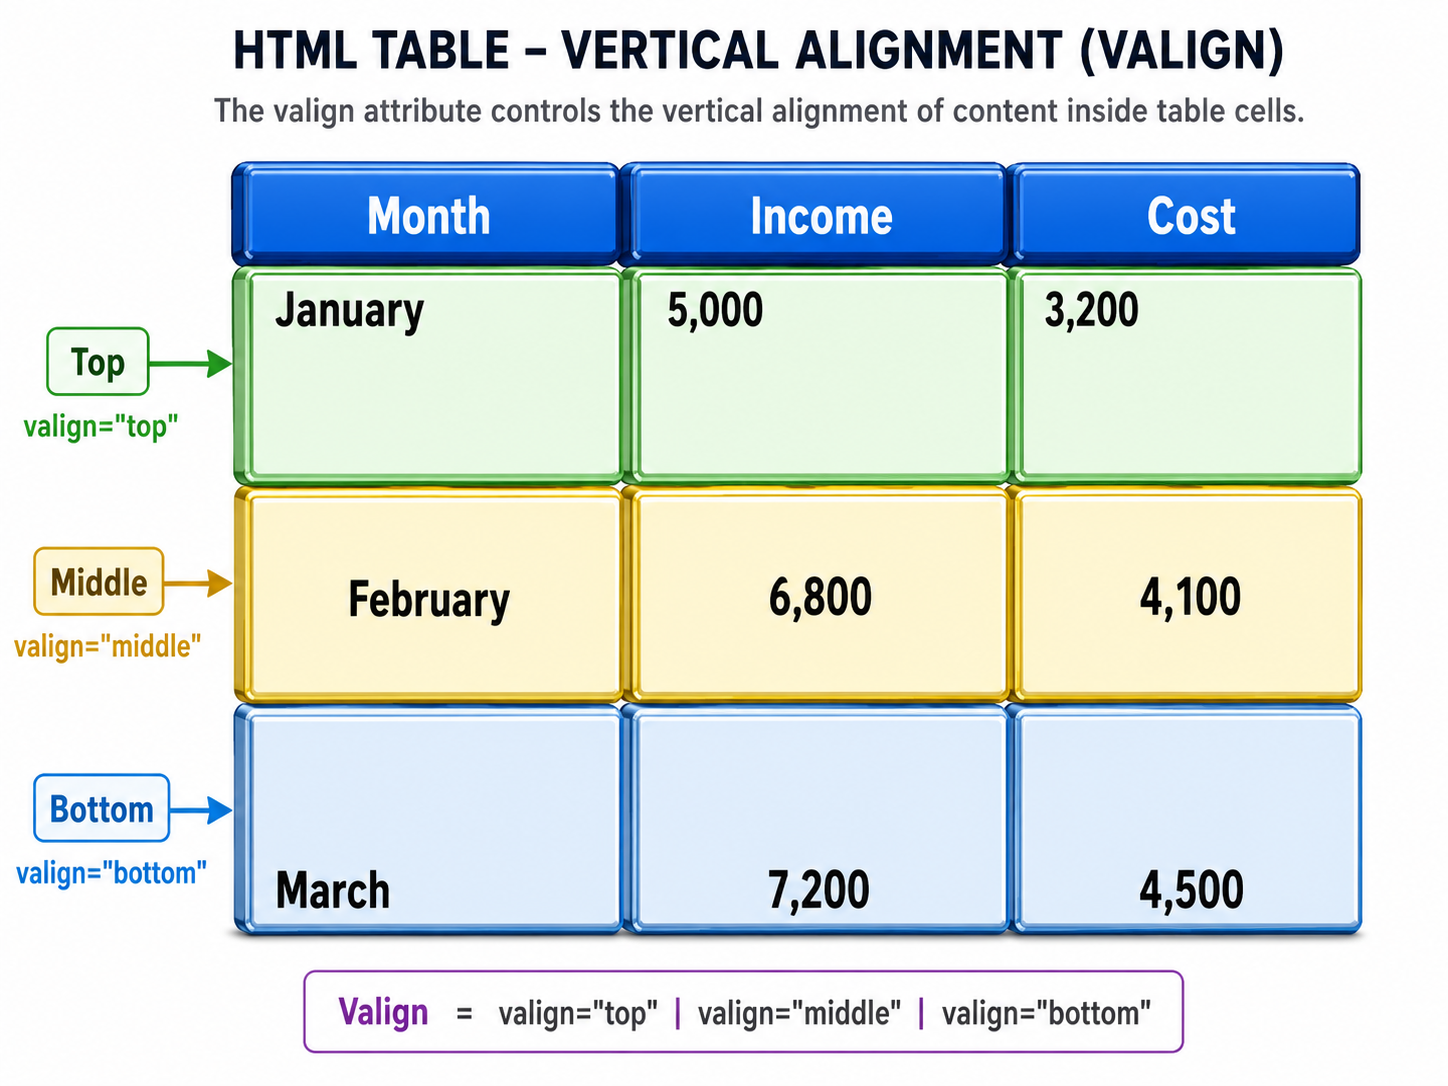
\includegraphics[width=0.95\linewidth,height=0.11\textheight,keepaspectratio]{chapters/Chapter04/topics/images/ex11_3d_valign_month_income_cost.png}
}{
\fbox{\parbox{0.90\linewidth}{\centering\vspace{0.4cm}
\textbf{চিত্র}\\
File: \texttt{chapters/Chapter04/topics/images/ex11\_3d\_valign\_month\_income\_cost.png}
\vspace{0.4cm}}}
}
\captionof{figure}{Exercise 11-এর valign চিত্র}
\end{center}

\begin{keypointbox}{চিত্র ব্যাখ্যা}
চিত্রে Month, Income ও Cost table দেখানো হয়েছে। January row top, February row middle এবং March row bottom vertical alignment বোঝায়।
\end{keypointbox}

\begin{keypointbox}{চিত্র দেখে code লেখার ধাপ}
প্রথম row-তে \texttt{valign="top"}, দ্বিতীয় row-তে \texttt{valign="middle"}, তৃতীয় row-তে \texttt{valign="bottom"} ব্যবহার করবে।
\end{keypointbox}

\par\noindent{\color{purple!70!black}\bfseries\small কোড}\par\vspace{-4pt}
\begin{verbatim}
<!DOCTYPE html>
<html>
<head>
  <title>HTML Table Example</title>
</head>
<body>
<table border="1" cellspacing="0" cellpadding="8">
  <tr><th>Month</th><th>Income</th><th>Cost</th></tr>
  <tr valign="top" height="60"><td>January</td><td>5,000</td><td>3,200</td></tr>
  <tr valign="middle" height="60"><td>February</td><td>6,800</td><td>4,100</td></tr>
  <tr valign="bottom" height="60"><td>March</td><td>7,200</td><td>4,500</td></tr>
</table>
</body>
</html>
\end{verbatim}
\vspace{-6pt}

\subsubsection{Exercise 12: Colgroup দিয়ে Column Color}

\begin{boardbox}{Concept}
\texttt{<colgroup>} ও \texttt{<col>} tag দিয়ে নির্দিষ্ট column-এর style দেওয়া যায়।
\end{boardbox}

\begin{center}
\IfFileExists{chapters/Chapter04/topics/images/ex12_3d_colgroup_color.png}{
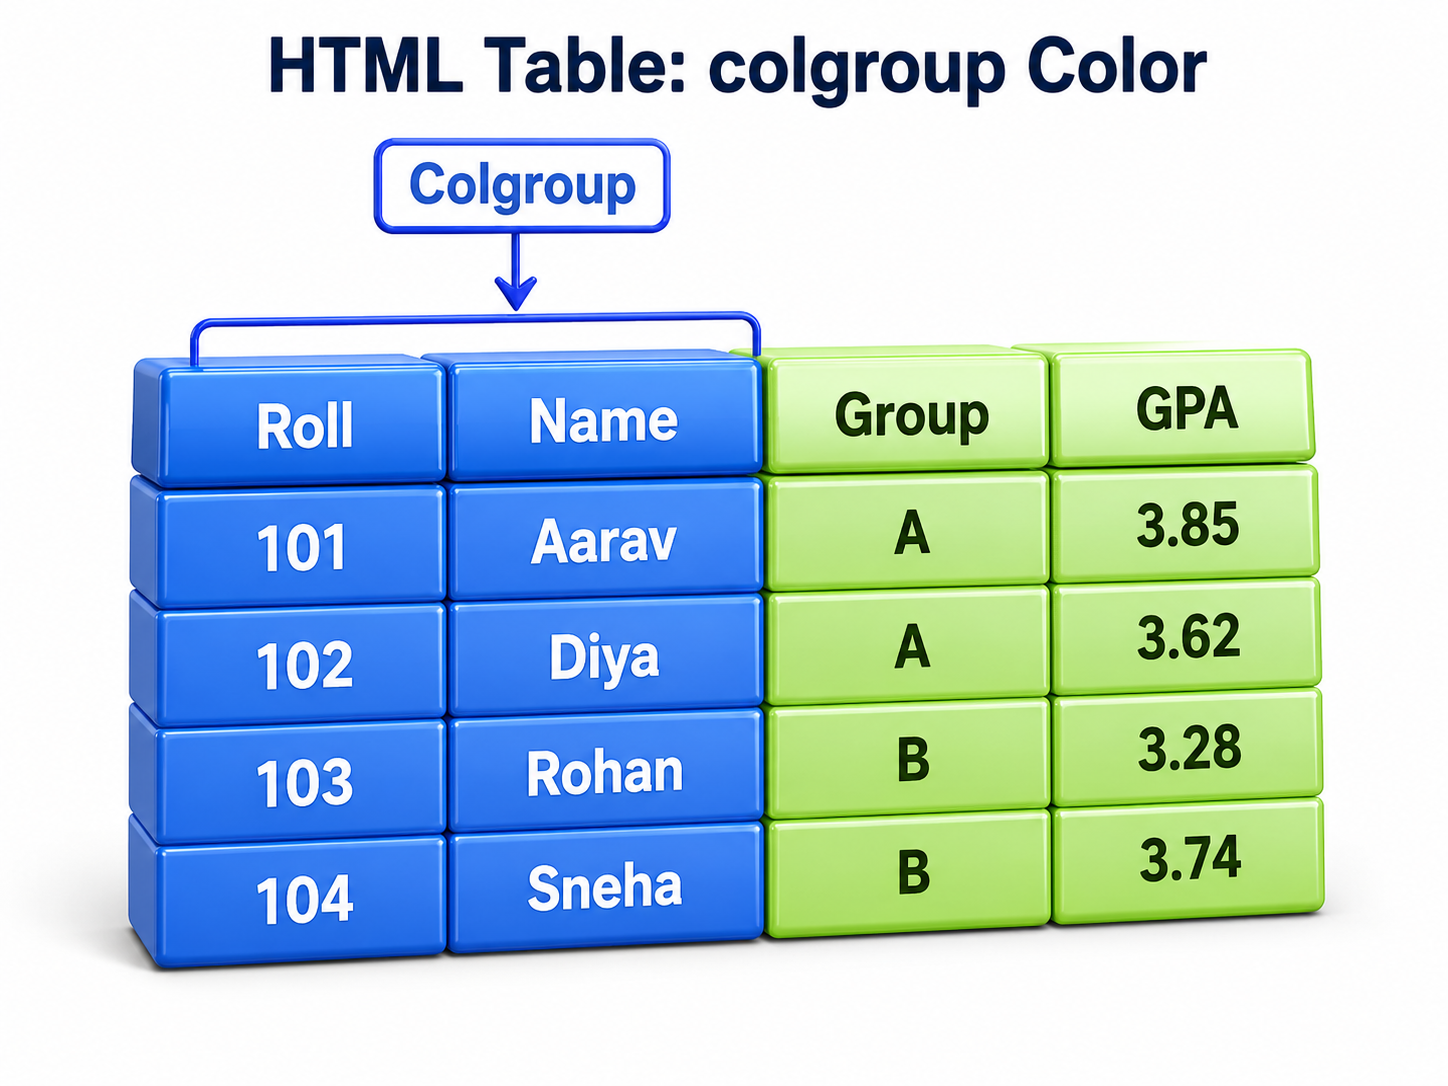
\includegraphics[width=0.95\linewidth,height=0.11\textheight,keepaspectratio]{chapters/Chapter04/topics/images/ex12_3d_colgroup_color.png}
}{
\fbox{\parbox{0.90\linewidth}{\centering\vspace{0.4cm}
\textbf{চিত্র}\\
File: \texttt{chapters/Chapter04/topics/images/ex12\_3d\_colgroup\_color.png}
\vspace{0.4cm}}}
}
\captionof{figure}{Exercise 12-এর colgroup চিত্র}
\end{center}

\begin{keypointbox}{চিত্র ব্যাখ্যা}
চিত্রে Roll ও Name column এক রঙে এবং Group ও GPA column আরেক রঙে দেখানো হয়েছে। এটি colgroup দিয়ে column-based styling বোঝায়।
\end{keypointbox}

\begin{keypointbox}{চিত্র দেখে code লেখার ধাপ}
প্রথমে \texttt{<colgroup>} লিখবে। কোন column কোন color হবে তা \texttt{<col span="...">} দিয়ে নির্ধারণ করবে। তারপর normal table row লিখবে।
\end{keypointbox}

\par\noindent{\color{purple!70!black}\bfseries\small কোড}\par\vspace{-4pt}
\begin{verbatim}
<!DOCTYPE html>
<html>
<head>
  <title>HTML Table Example</title>
</head>
<body>
<table border="1" cellspacing="0" cellpadding="6">
  <colgroup>
    <col span="2" style="background-color:#77b7ff">
    <col span="2" style="background-color:#b7ef7a">
  </colgroup>
  <tr><th>Roll</th><th>Name</th><th>Group</th><th>GPA</th></tr>
  <tr><td>101</td><td>Aarav</td><td>A</td><td>3.85</td></tr>
  <tr><td>102</td><td>Diya</td><td>A</td><td>3.62</td></tr>
  <tr><td>103</td><td>Rohan</td><td>B</td><td>3.28</td></tr>
  <tr><td>104</td><td>Sneha</td><td>B</td><td>3.74</td></tr>
</table>
</body>
</html>
\end{verbatim}
\vspace{-6pt}

\subsubsection{Exercise 13: Without Cellspacing and With Cellspacing}

\begin{boardbox}{Concept}
\texttt{cellspacing} cell-এর বাইরের gap বা cellগুলোর মাঝের distance নিয়ন্ত্রণ করে।
\end{boardbox}

\begin{center}
\IfFileExists{chapters/Chapter04/topics/images/ex13_3d_cellspacing_compare.png}{
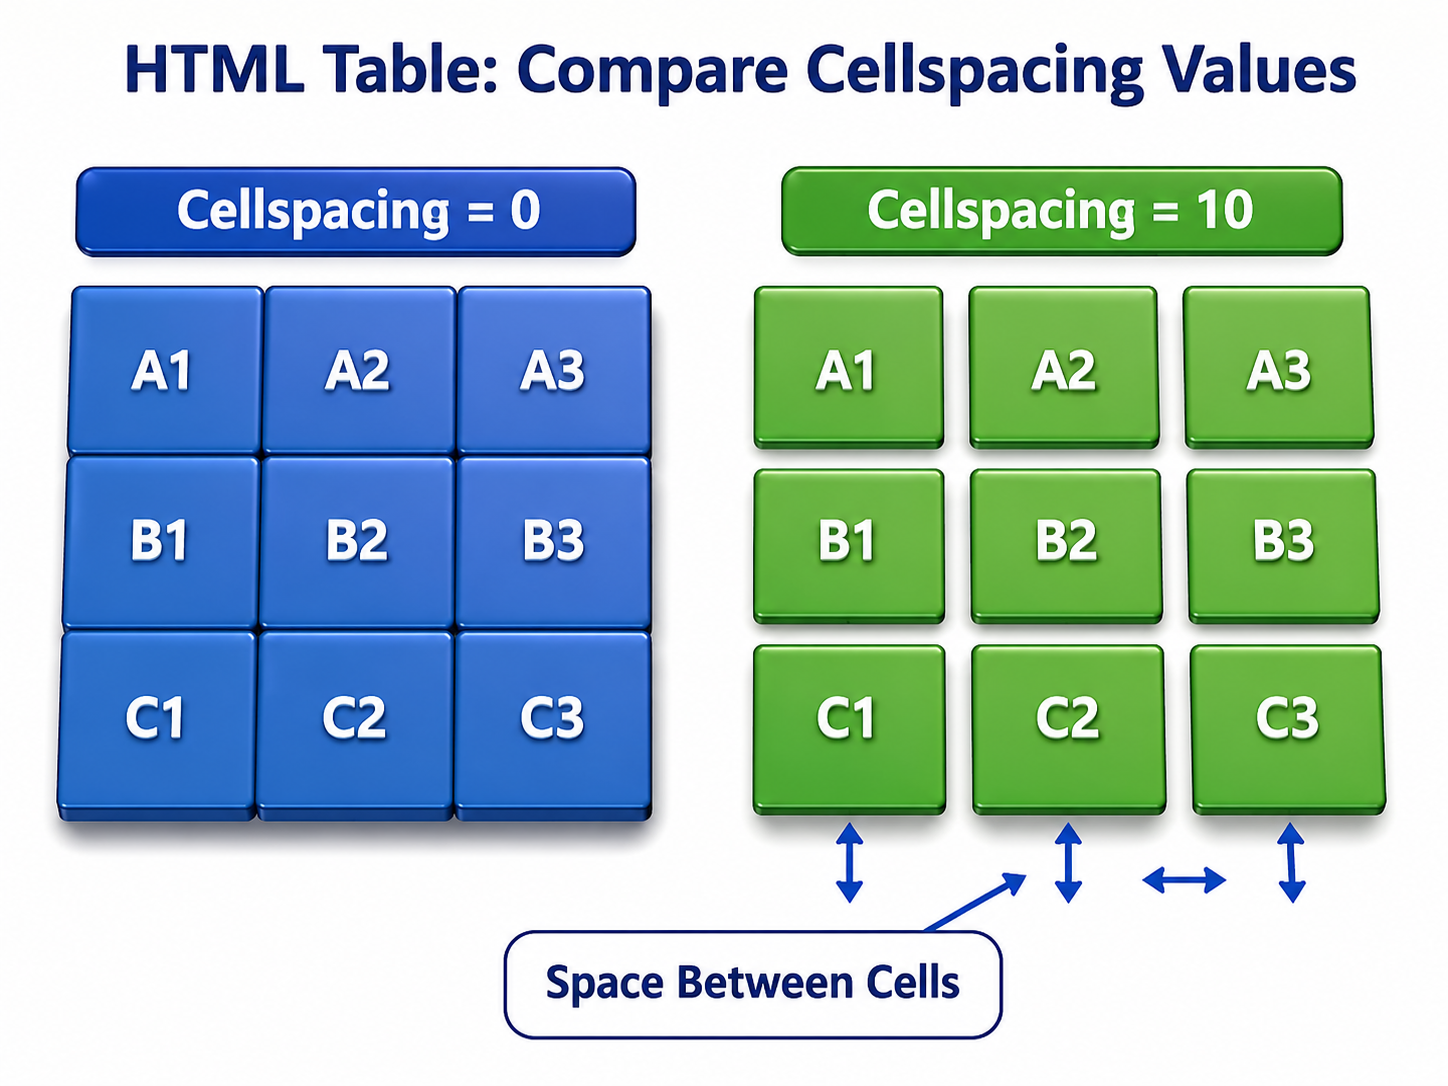
\includegraphics[width=0.95\linewidth,height=0.11\textheight,keepaspectratio]{chapters/Chapter04/topics/images/ex13_3d_cellspacing_compare.png}
}{
\fbox{\parbox{0.90\linewidth}{\centering\vspace{0.4cm}
\textbf{চিত্র}\\
File: \texttt{chapters/Chapter04/topics/images/ex13\_3d\_cellspacing\_compare.png}
\vspace{0.4cm}}}
}
\captionof{figure}{Exercise 13-এর cellspacing তুলনা}
\end{center}

\begin{keypointbox}{চিত্র ব্যাখ্যা}
চিত্রে বাম table-এ \texttt{cellspacing="0"} থাকায় cellগুলোর মাঝে gap নেই। ডান table-এ \texttt{cellspacing="10"} থাকায় cellগুলোর মাঝে space দেখা যাচ্ছে।
\end{keypointbox}

\begin{keypointbox}{চিত্র দেখে code লেখার ধাপ}
একই data দিয়ে দুটি table লিখবে। প্রথমটিতে \texttt{cellspacing="0"} এবং দ্বিতীয়টিতে \texttt{cellspacing="10"} ব্যবহার করবে।
\end{keypointbox}

\par\noindent{\color{purple!70!black}\bfseries\small কোড}\par\vspace{-4pt}
\begin{verbatim}
<!DOCTYPE html>
<html>
<head>
  <title>HTML Table Example</title>
</head>
<body>
<h3>Cellspacing = 0</h3>
<table border="1" cellspacing="0" cellpadding="8">
  <tr><td>A1</td><td>A2</td><td>A3</td></tr>
  <tr><td>B1</td><td>B2</td><td>B3</td></tr>
  <tr><td>C1</td><td>C2</td><td>C3</td></tr>
</table>

<h3>Cellspacing = 10</h3>
<table border="1" cellspacing="10" cellpadding="8">
  <tr><td>A1</td><td>A2</td><td>A3</td></tr>
  <tr><td>B1</td><td>B2</td><td>B3</td></tr>
  <tr><td>C1</td><td>C2</td><td>C3</td></tr>
</table>
</body>
</html>
\end{verbatim}
\vspace{-6pt}

\subsubsection{Exercise 14: Without Cellpadding and With Cellpadding}

\begin{boardbox}{Concept}
\texttt{cellpadding} cell-এর border এবং content-এর মাঝের ভিতরের space নিয়ন্ত্রণ করে।
\end{boardbox}

\begin{center}
\IfFileExists{chapters/Chapter04/topics/images/ex14_3d_cellpadding_compare.png}{
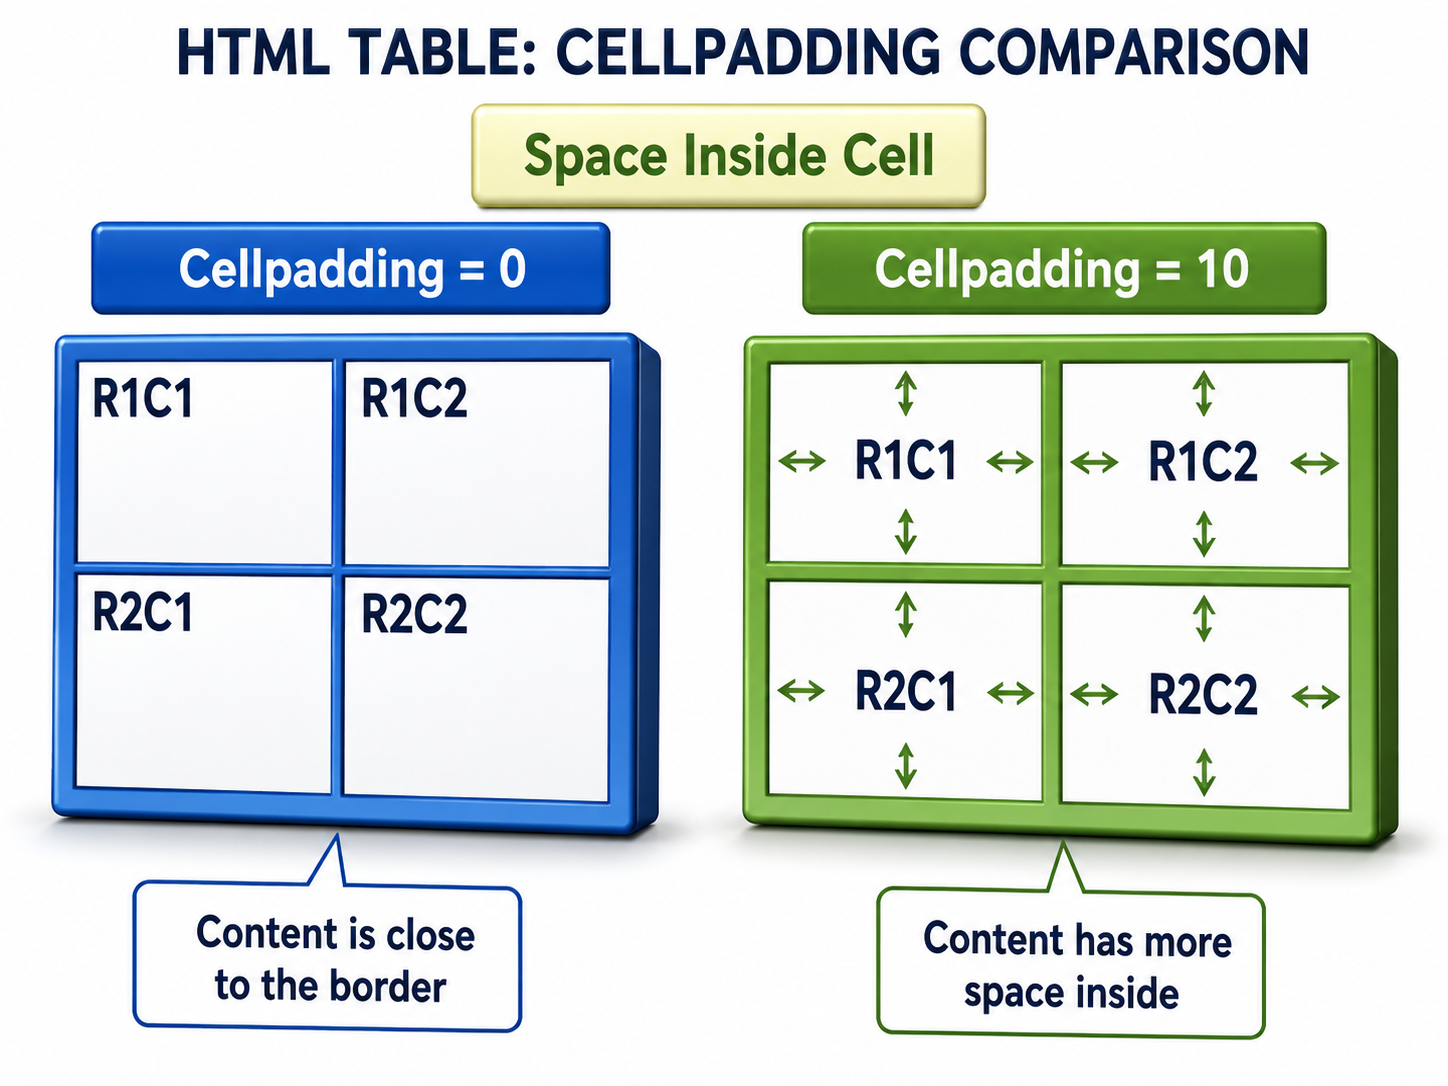
\includegraphics[width=0.95\linewidth,height=0.11\textheight,keepaspectratio]{chapters/Chapter04/topics/images/ex14_3d_cellpadding_compare.png}
}{
\fbox{\parbox{0.90\linewidth}{\centering\vspace{0.4cm}
\textbf{চিত্র}\\
File: \texttt{chapters/Chapter04/topics/images/ex14\_3d\_cellpadding\_compare.png}
\vspace{0.4cm}}}
}
\captionof{figure}{Exercise 14-এর cellpadding তুলনা}
\end{center}

\begin{keypointbox}{চিত্র ব্যাখ্যা}
চিত্রে বাম table-এ \texttt{cellpadding="0"} থাকায় content border-এর কাছে আছে। ডান table-এ \texttt{cellpadding="10"} থাকায় content-এর চারপাশে ভিতরের space বেশি।
\end{keypointbox}

\begin{keypointbox}{চিত্র দেখে code লেখার ধাপ}
দুটি table তৈরি করবে। প্রথম table-এ \texttt{cellpadding="0"}, দ্বিতীয় table-এ \texttt{cellpadding="10"} বসাবে।
\end{keypointbox}

\par\noindent{\color{purple!70!black}\bfseries\small কোড}\par\vspace{-4pt}
\begin{verbatim}
<!DOCTYPE html>
<html>
<head>
  <title>HTML Table Example</title>
</head>
<body>
<h3>Cellpadding = 0</h3>
<table border="1" cellspacing="0" cellpadding="0">
  <tr><td>R1C1</td><td>R1C2</td></tr>
  <tr><td>R2C1</td><td>R2C2</td></tr>
</table>

<h3>Cellpadding = 10</h3>
<table border="1" cellspacing="0" cellpadding="10">
  <tr><td>R1C1</td><td>R1C2</td></tr>
  <tr><td>R2C1</td><td>R2C2</td></tr>
</table>
</body>
</html>
\end{verbatim}
\vspace{-6pt}

\subsubsection{Exercise 15: Caption Tag Practice}

\begin{boardbox}{Concept}
\texttt{<caption>} table-এর উপরে title দেখায়। border value বাড়ালে border visually thick দেখায়।
\end{boardbox}

\begin{center}
\IfFileExists{chapters/Chapter04/topics/images/ex15_3d_caption_thick_border.png}{
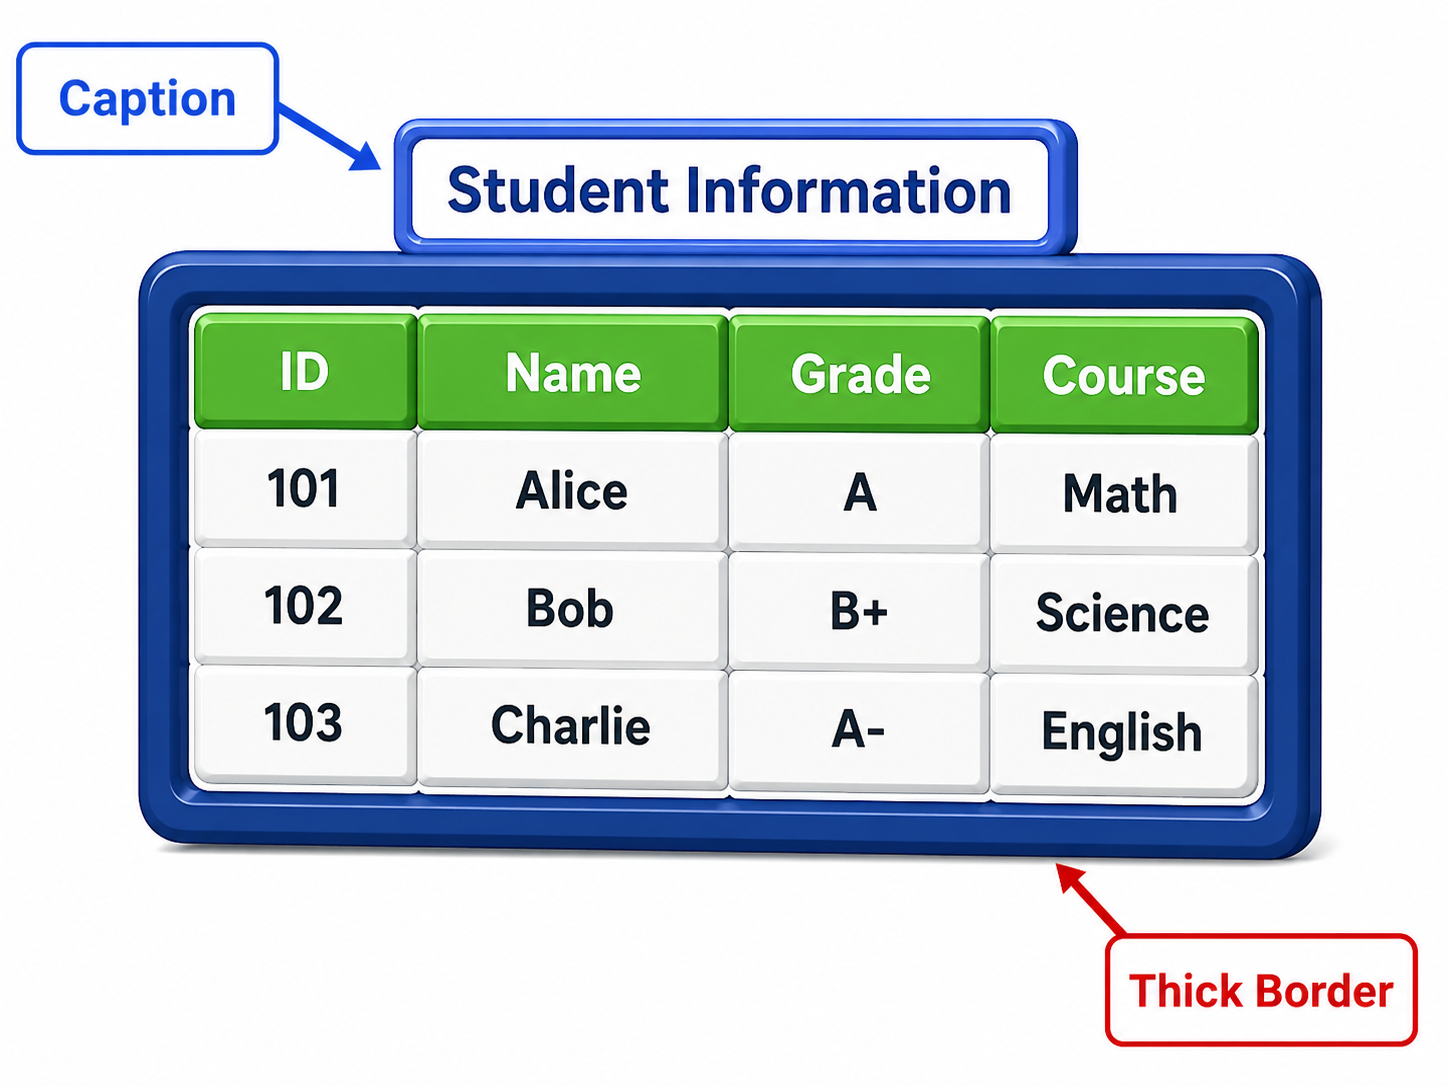
\includegraphics[width=0.95\linewidth,height=0.11\textheight,keepaspectratio]{chapters/Chapter04/topics/images/ex15_3d_caption_thick_border.png}
}{
\fbox{\parbox{0.90\linewidth}{\centering\vspace{0.4cm}
\textbf{চিত্র}\\
File: \texttt{chapters/Chapter04/topics/images/ex15\_3d\_caption\_thick\_border.png}
\vspace{0.4cm}}}
}
\captionof{figure}{Exercise 15-এর caption চিত্র}
\end{center}

\begin{keypointbox}{চিত্র ব্যাখ্যা}
চিত্রে Student Information caption এবং thick border সহ ID, Name, Grade ও Course column দেখানো হয়েছে।
\end{keypointbox}

\begin{keypointbox}{চিত্র দেখে code লেখার ধাপ}
প্রথমে table tag-এ border বসাবে। তারপর \texttt{<caption>} দিয়ে Student Information লিখবে। এরপর header row ও data rows লিখবে।
\end{keypointbox}

\par\noindent{\color{purple!70!black}\bfseries\small কোড}\par\vspace{-4pt}
\begin{verbatim}
<!DOCTYPE html>
<html>
<head>
  <title>HTML Table Example</title>
</head>
<body>
<table border="4" cellspacing="0" cellpadding="6">
  <caption><b>Student Information</b></caption>
  <tr><th>ID</th><th>Name</th><th>Grade</th><th>Course</th></tr>
  <tr><td>101</td><td>Alice</td><td>A</td><td>Math</td></tr>
  <tr><td>102</td><td>Bob</td><td>B+</td><td>Science</td></tr>
  <tr><td>103</td><td>Charlie</td><td>A-</td><td>English</td></tr>
</table>
</body>
</html>
\end{verbatim}
\vspace{-6pt}

\subsubsection{Exercise 16: Bio-data Table with Next Link}

\begin{boardbox}{Concept}
Table cell-এর ভিতরে hyperlink রাখা যায়। Bio-data table-এ label এবং value দুই column হিসেবে সাজানো হয়।
\end{boardbox}

\begin{center}
\IfFileExists{chapters/Chapter04/topics/images/ex16_3d_biodata_link.png}{
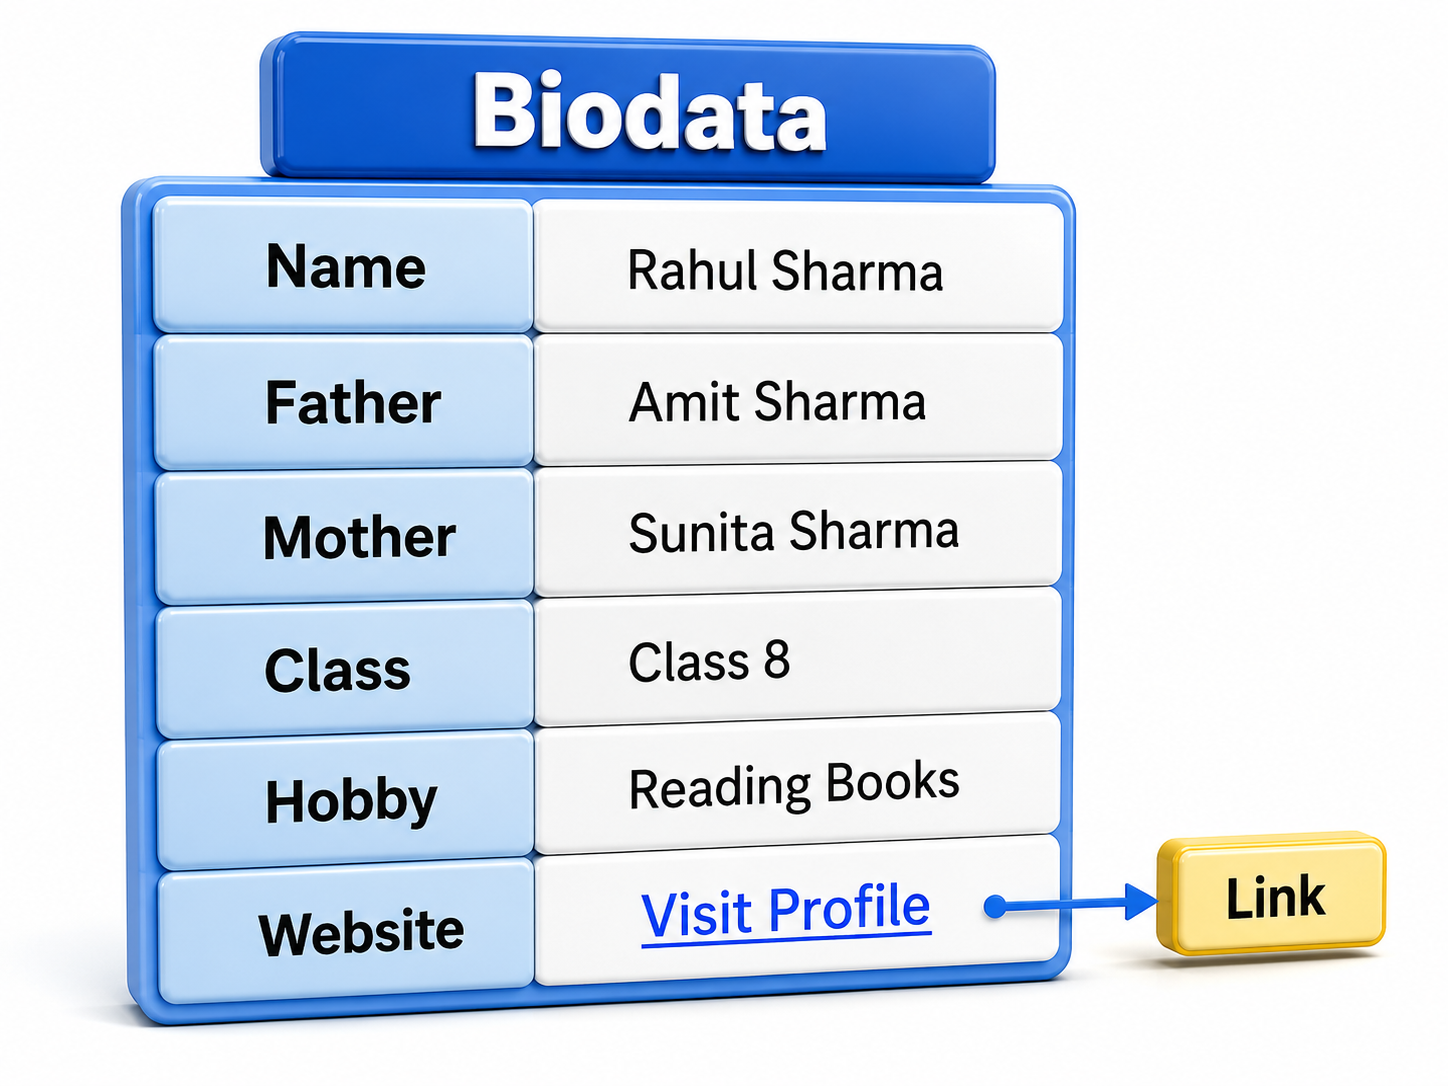
\includegraphics[width=0.95\linewidth,height=0.11\textheight,keepaspectratio]{chapters/Chapter04/topics/images/ex16_3d_biodata_link.png}
}{
\fbox{\parbox{0.90\linewidth}{\centering\vspace{0.4cm}
\textbf{চিত্র}\\
File: \texttt{chapters/Chapter04/topics/images/ex16\_3d\_biodata\_link.png}
\vspace{0.4cm}}}
}
\captionof{figure}{Exercise 16-এর biodata table চিত্র}
\end{center}

\begin{keypointbox}{চিত্র ব্যাখ্যা}
চিত্রে Biodata heading-এর নিচে Name, Father, Mother, Class, Hobby এবং Website row আছে। Website row-তে Visit Profile hyperlink দেখানো হয়েছে।
\end{keypointbox}

\begin{keypointbox}{চিত্র দেখে code লেখার ধাপ}
প্রথমে title row দুই column জুড়ে দিতে \texttt{colspan="2"} ব্যবহার করবে। তারপর প্রতিটি label-value row লিখবে। Website cell-এ \texttt{<a>} tag দিয়ে link তৈরি করবে।
\end{keypointbox}

\par\noindent{\color{purple!70!black}\bfseries\small কোড}\par\vspace{-4pt}
\begin{verbatim}
<!DOCTYPE html>
<html>
<head>
  <title>HTML Table Example</title>
</head>
<body>
<table border="1" cellspacing="0" cellpadding="6" align="center">
  <tr><th colspan="2">Biodata</th></tr>
  <tr><th>Name</th><td>Rahul Sharma</td></tr>
  <tr><th>Father</th><td>Amit Sharma</td></tr>
  <tr><th>Mother</th><td>Sunita Sharma</td></tr>
  <tr><th>Class</th><td>Class 8</td></tr>
  <tr><th>Hobby</th><td>Reading Books</td></tr>
  <tr><th>Website</th><td><a href="profile.html">Visit Profile</a></td></tr>
</table>
</body>
</html>
\end{verbatim}
\vspace{-6pt}
\subsubsection{Exercise 17: Mobile Company Table}

\begin{center}
\IfFileExists{chapters/Chapter04/topics/images/ex17_3d_mobile_company.png}{
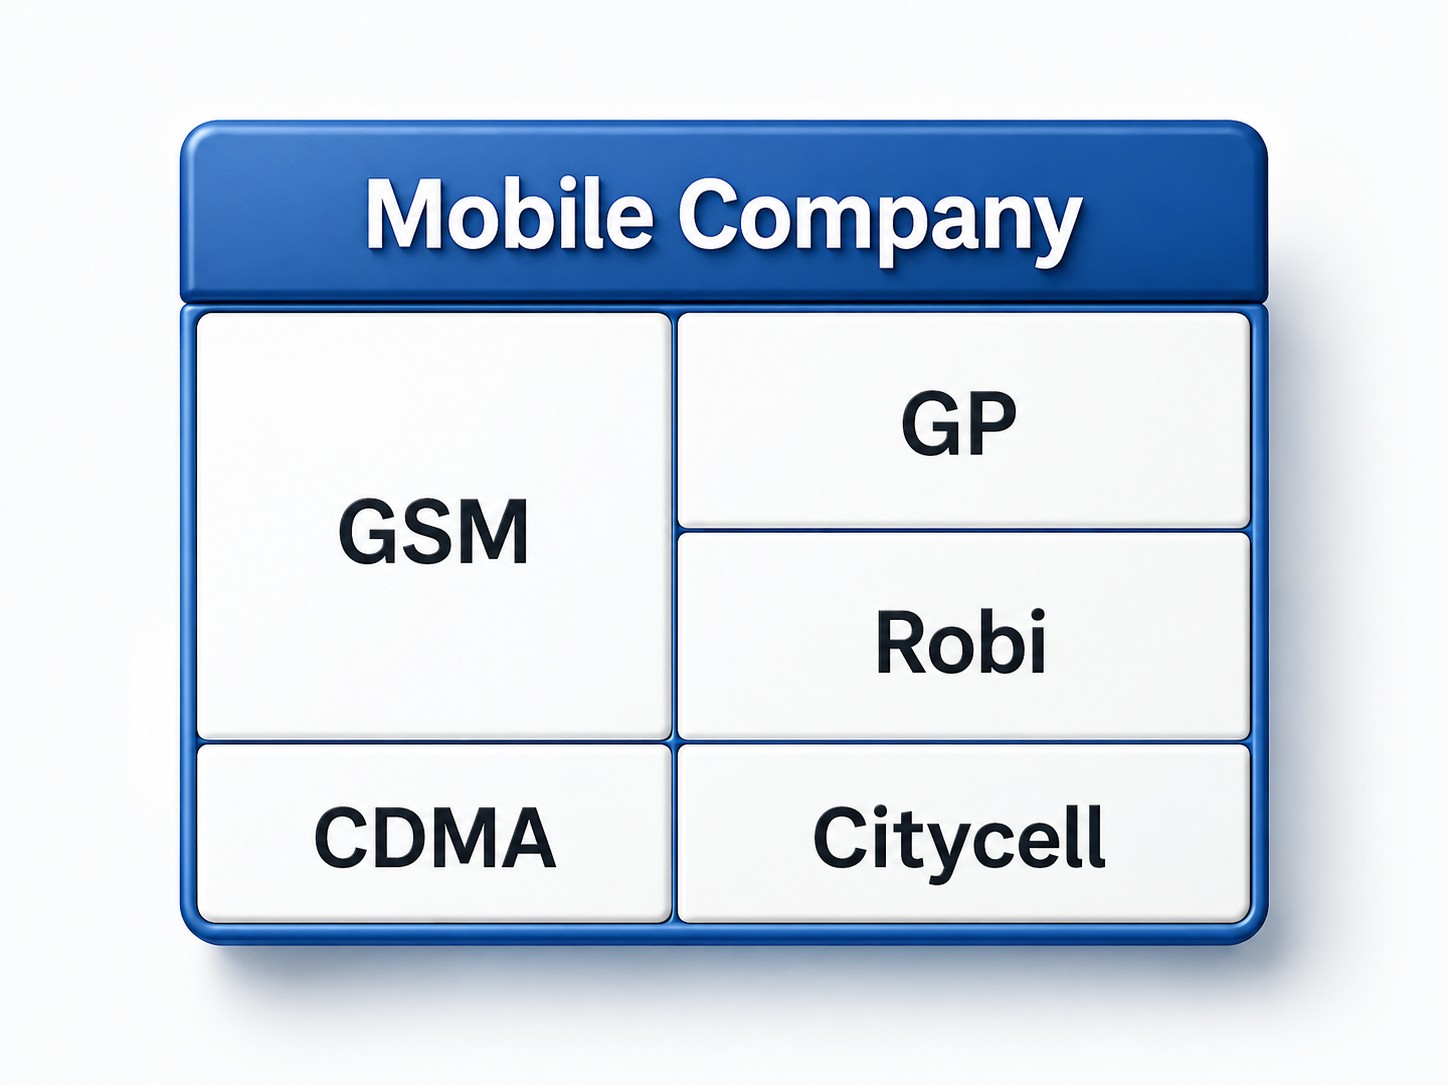
\includegraphics[width=0.95\linewidth,height=0.11\textheight,keepaspectratio]{chapters/Chapter04/topics/images/ex17_3d_mobile_company.png}
}{
\fbox{\parbox{0.90\linewidth}{\centering\vspace{0.45cm}
\textbf{চিত্র}\\[3pt]
File: \texttt{chapters/Chapter04/topics/images/ex17\_3d\_mobile\_company.png}
\vspace{0.45cm}}}
}
\captionof{figure}{Mobile Company table with rowspan}
\end{center}

\begin{keypointbox}{চিত্র ব্যাখ্যা}
GSM cell দুই row জুড়ে আছে। তাই GP ও Robi একই GSM category-এর অধীনে দেখানো হয়েছে। CDMA ও Citycell শেষ row-তে আছে।
\end{keypointbox}

\begin{keypointbox}{চিত্র দেখে code লেখার ধাপ}
প্রথমে figure-এর total row ও column গুনবে। এরপর কোন cell একাধিক column জুড়ে আছে তা দেখে \texttt{colspan} এবং কোন cell একাধিক row জুড়ে আছে তা দেখে \texttt{rowspan} বসাবে। তারপর image, link, list বা nested table থাকলে সংশ্লিষ্ট tag cell-এর ভিতরে লিখবে।
\end{keypointbox}

\par\noindent{\color{purple!70!black}\bfseries\small কোড}\par\vspace{-4pt}
\begin{verbatim}
<!DOCTYPE html>
<html>
<head>
  <title>HTML Table Example</title>
</head>
<body>
<table border="1" cellspacing="0">
<caption>Mobile Company</caption>
<tr>
  <td rowspan="2">GSM</td>
  <td>GP</td>
</tr>
<tr>
  <td>Robi</td>
</tr>
<tr>
  <td>CDMA</td>
  <td>Citycell</td>
</tr>
</table>
</body>
</html>
\end{verbatim}
\vspace{-6pt}

\subsubsection{Exercise 18: Complex Number Grid with Rowspan and Colspan}

\begin{center}
\IfFileExists{chapters/Chapter04/topics/images/ex18_3d_complex_number_grid.png}{
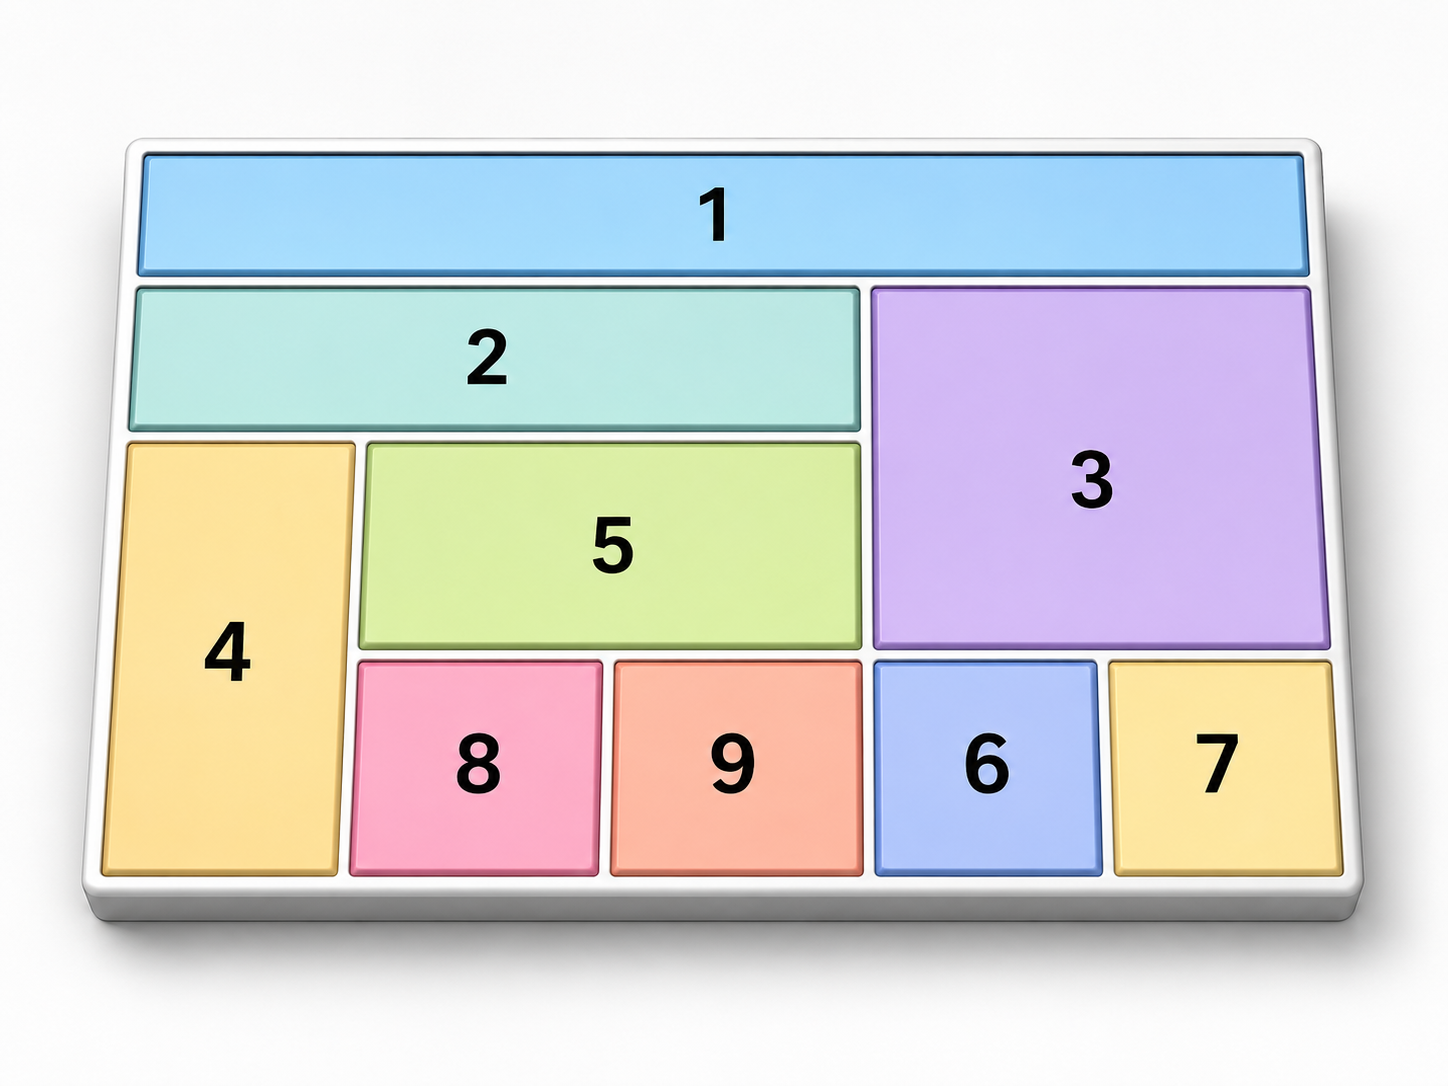
\includegraphics[width=0.95\linewidth,height=0.11\textheight,keepaspectratio]{chapters/Chapter04/topics/images/ex18_3d_complex_number_grid.png}
}{
\fbox{\parbox{0.90\linewidth}{\centering\vspace{0.45cm}
\textbf{চিত্র}\\[3pt]
File: \texttt{chapters/Chapter04/topics/images/ex18\_3d\_complex\_number\_grid.png}
\vspace{0.45cm}}}
}
\captionof{figure}{Complex number grid with rowspan and colspan}
\end{center}

\begin{keypointbox}{চিত্র ব্যাখ্যা}
এই table-এ 1, 2, 3, 4, 5, 8, 9 cell-এ rowspan/colspan ব্যবহার করা হয়েছে। চিত্র দেখে code লেখার জন্য এটি খুব গুরুত্বপূর্ণ practice।
\end{keypointbox}

\par\noindent{\color{purple!70!black}\bfseries\small কোড}\par\vspace{-4pt}
\begin{verbatim}
<!DOCTYPE html>
<html>
<head>
  <title>HTML Table Example</title>
</head>
<body>
<table border="1" cellspacing="0">
<tr><td colspan="5">1</td></tr>
<tr><td colspan="3">2</td><td colspan="2" rowspan="3">3</td></tr>
<tr><td rowspan="3">4</td><td colspan="2">5</td></tr>
<tr><td rowspan="2">8</td><td rowspan="2">9</td></tr>
<tr><td>6</td><td>7</td></tr>
</table>
</body>
</html>
\end{verbatim}
\vspace{-6pt}

\subsubsection{Exercise 19: Mymensingh Gov. College Group and Seats Table}

\begin{center}
\IfFileExists{chapters/Chapter04/topics/images/ex19_3d_mgc_group_seats.png}{
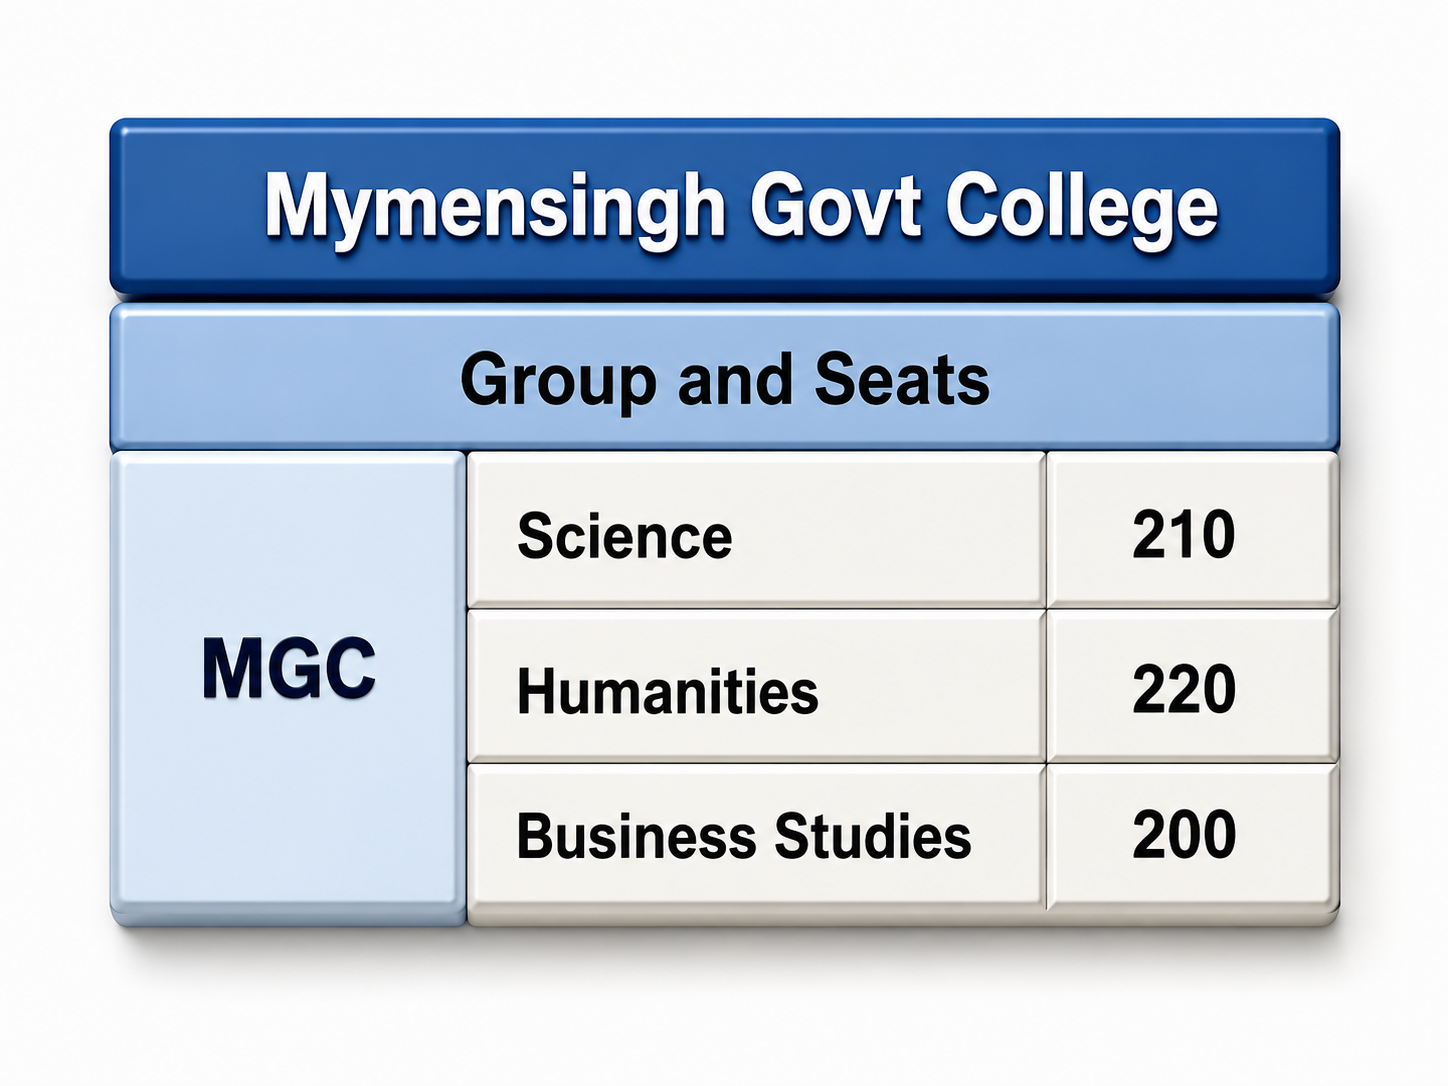
\includegraphics[width=0.95\linewidth,height=0.11\textheight,keepaspectratio]{chapters/Chapter04/topics/images/ex19_3d_mgc_group_seats.png}
}{
\fbox{\parbox{0.90\linewidth}{\centering\vspace{0.45cm}
\textbf{চিত্র}\\[3pt]
File: \texttt{chapters/Chapter04/topics/images/ex19\_3d\_mgc\_group\_seats.png}
\vspace{0.45cm}}}
}
\captionof{figure}{Mymensingh Govt. College group and seats table}
\end{center}

\begin{keypointbox}{চিত্র ব্যাখ্যা}
MGC cell তিনটি group row জুড়ে আছে। Group and Seats heading তিনটি column জুড়ে আছে।
\end{keypointbox}

\begin{keypointbox}{চিত্র দেখে code লেখার ধাপ}
প্রথমে figure-এর total row ও column গুনবে। এরপর কোন cell একাধিক column জুড়ে আছে তা দেখে \texttt{colspan} এবং কোন cell একাধিক row জুড়ে আছে তা দেখে \texttt{rowspan} বসাবে। তারপর image, link, list বা nested table থাকলে সংশ্লিষ্ট tag cell-এর ভিতরে লিখবে।
\end{keypointbox}

\par\noindent{\color{purple!70!black}\bfseries\small কোড}\par\vspace{-4pt}
\begin{verbatim}
<!DOCTYPE html>
<html>
<head>
  <title>HTML Table Example</title>
</head>
<body>
<p align="center"><h2>Mymensingh Govt College</h2></p>
<table border="1" cellspacing="0" cellpadding="10">
<tr><th colspan="3">Group and Seats</th></tr>
<tr><td rowspan="3">MGC</td><td>Science</td><td>210</td></tr>
<tr><td>Humanities</td><td>220</td></tr>
<tr><td>Business Studies</td><td>200</td></tr>
</table>
</body>
</html>
\end{verbatim}
\vspace{-6pt}

\subsubsection{Exercise 20: Product Table with Image}

\begin{center}
\IfFileExists{chapters/Chapter04/topics/images/ex20_3d_product_image.png}{
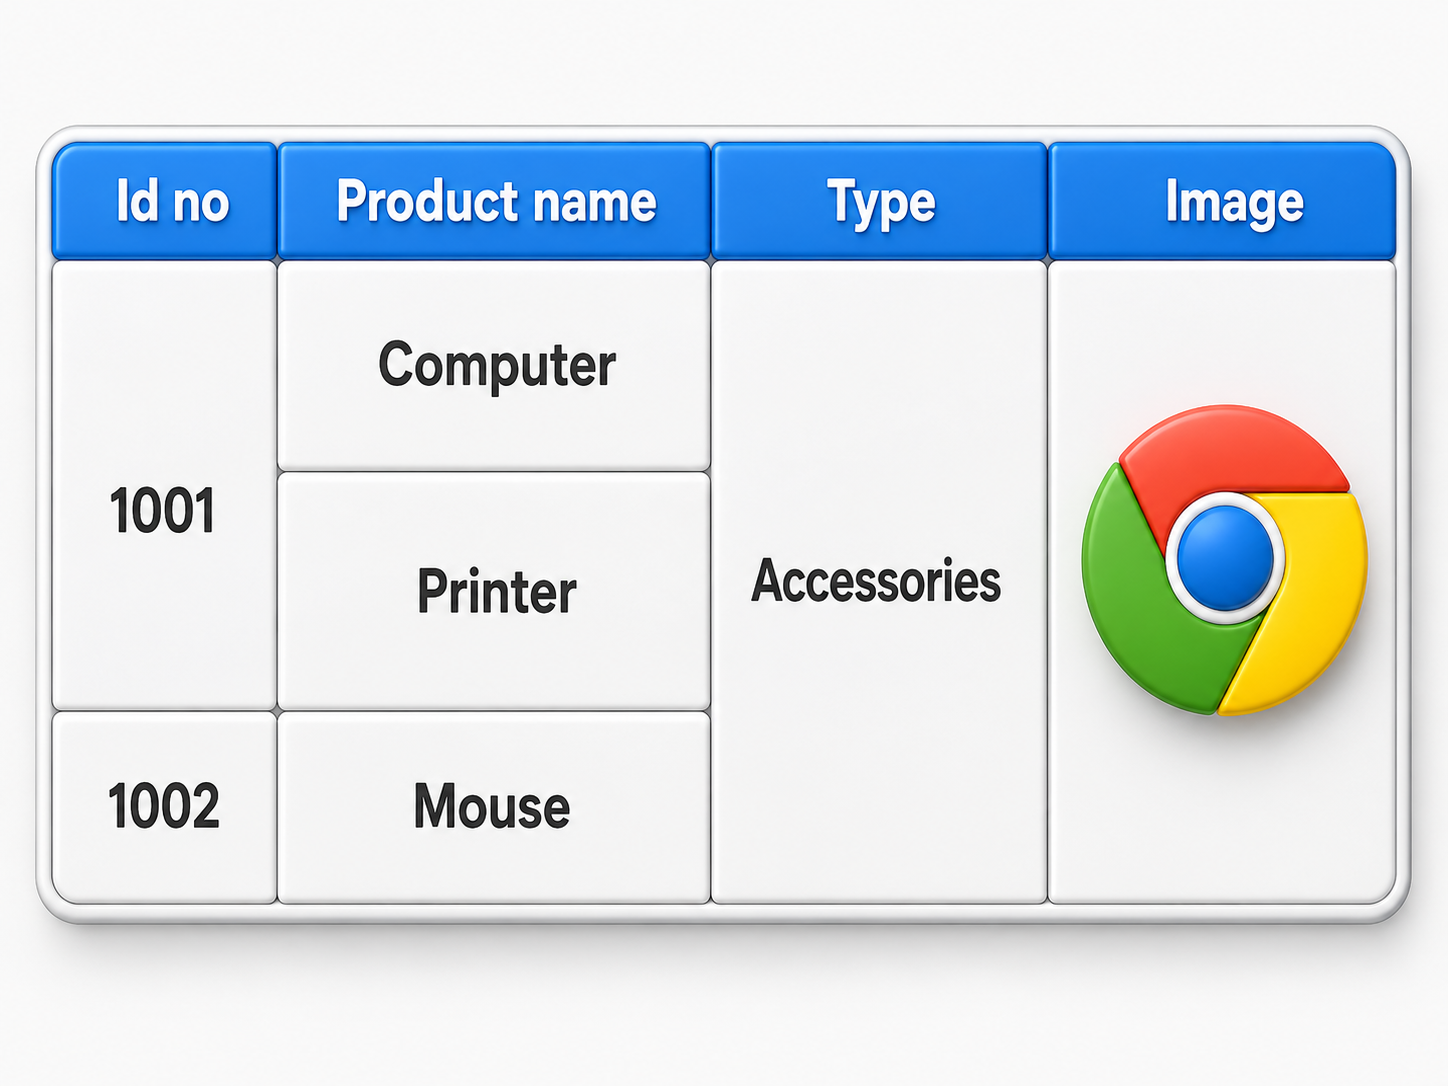
\includegraphics[width=0.95\linewidth,height=0.11\textheight,keepaspectratio]{chapters/Chapter04/topics/images/ex20_3d_product_image.png}
}{
\fbox{\parbox{0.90\linewidth}{\centering\vspace{0.45cm}
\textbf{চিত্র}\\[3pt]
File: \texttt{chapters/Chapter04/topics/images/ex20\_3d\_product\_image.png}
\vspace{0.45cm}}}
}
\captionof{figure}{Product table with rowspan and image}
\end{center}

\begin{keypointbox}{চিত্র ব্যাখ্যা}
এই table-এ image column-এর header cell চার row জুড়ে আছে। 1001 ID দুই product row জুড়ে এবং Accessories type তিন product row জুড়ে আছে।
\end{keypointbox}

\par\noindent{\color{purple!70!black}\bfseries\small কোড}\par\vspace{-4pt}
\begin{verbatim}
<!DOCTYPE html>
<html>
<head>
  <title>HTML Table Example</title>
</head>
<body>
<table border="1" cellspacing="0">
<tr>
  <th bgcolor="Silver">Id no</th>
  <th bgcolor="Silver">Product name</th>
  <th bgcolor="Silver">Type</th>
  <th rowspan="4"><img src="google.jpg" width="60" height="50" align="center"></th>
</tr>
<tr>
  <td rowspan="2">1001</td>
  <td>Computer</td>
  <td rowspan="3">Accessories</td>
</tr>
<tr>
  <td>Printer</td>
</tr>
<tr>
  <td>1002</td>
  <td>Mouse</td>
</tr>
</table>
</body>
</html>
\end{verbatim}
\vspace{-6pt}

\subsubsection{Exercise 21: Bangladesh Number Table}

\begin{center}
\IfFileExists{chapters/Chapter04/topics/images/ex21_3d_bangladesh_number_table.png}{
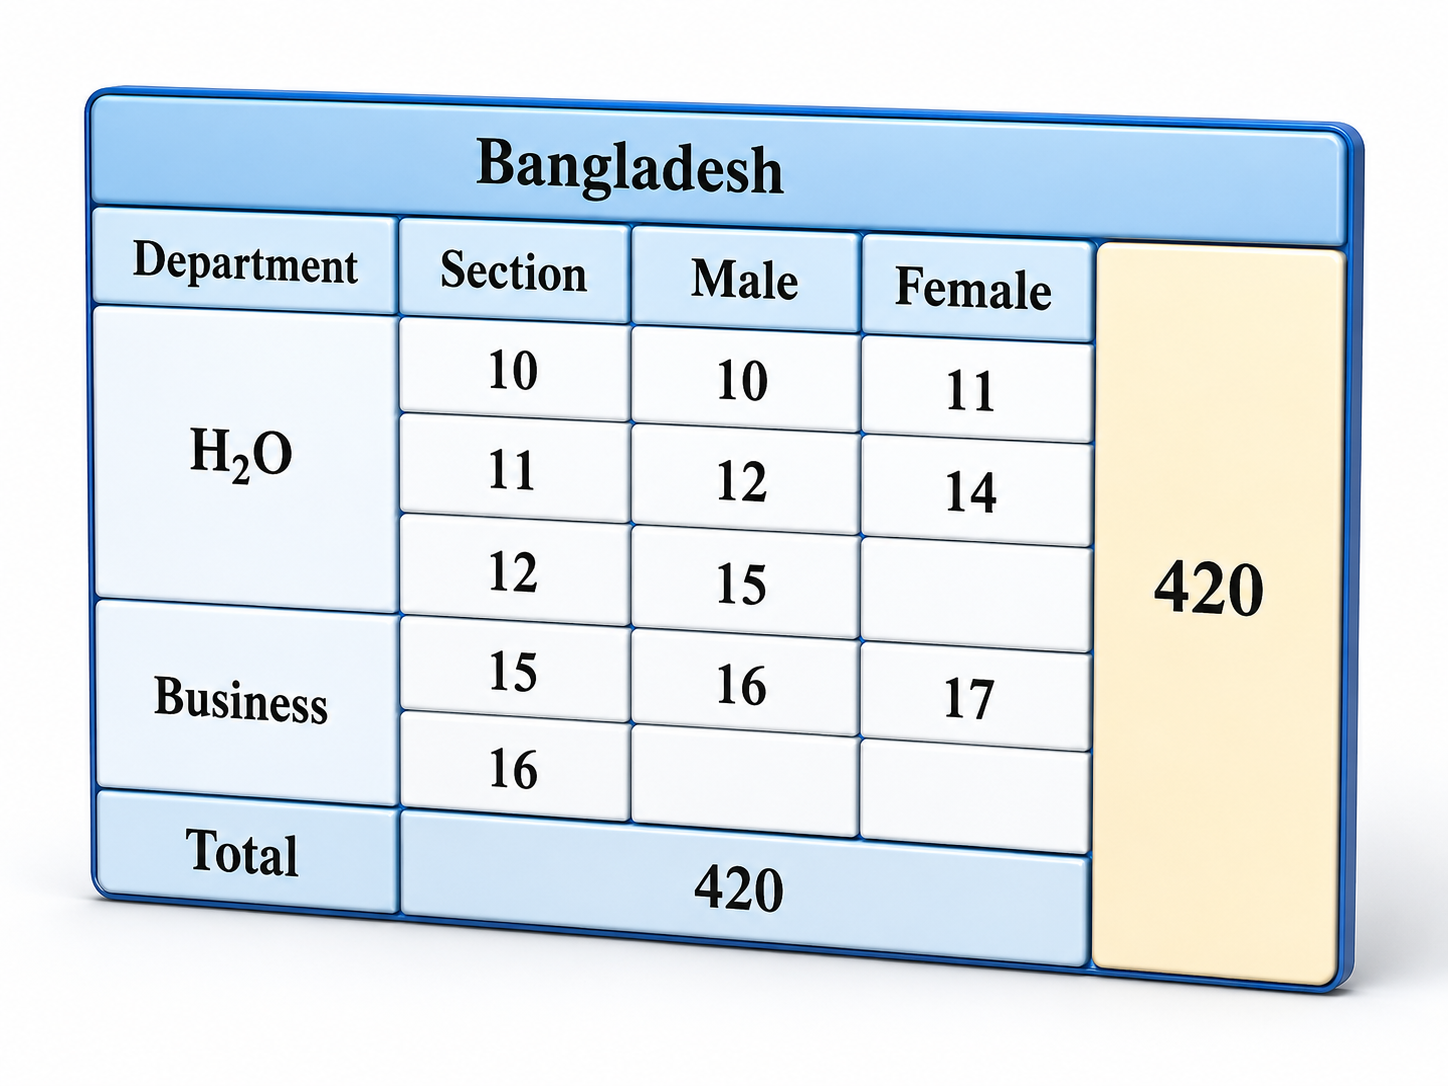
\includegraphics[width=0.95\linewidth,height=0.11\textheight,keepaspectratio]{chapters/Chapter04/topics/images/ex21_3d_bangladesh_number_table.png}
}{
\fbox{\parbox{0.90\linewidth}{\centering\vspace{0.45cm}
\textbf{চিত্র}\\[3pt]
File: \texttt{chapters/Chapter04/topics/images/ex21\_3d\_bangladesh\_number\_table.png}
\vspace{0.45cm}}}
}
\captionof{figure}{Bangladesh department number table with rowspan and colspan}
\end{center}

\begin{keypointbox}{চিত্র ব্যাখ্যা}
চিত্রে Bangladesh নামে একটি department-wise number table আছে। ডান পাশের \texttt{420} cell পুরো data অংশ জুড়ে আছে, তাই এখানে \texttt{rowspan} ব্যবহার করা হয়েছে। নিচের Total row-তে total value একাধিক column জুড়ে দেখানো হয়েছে।
\end{keypointbox}

\begin{keypointbox}{চিত্র দেখে code লেখার ধাপ}
প্রথমে header row-এর column গুনবে: Department, Section, Male, Female এবং ডান পাশের total cell। এরপর H\textsubscript{2}O/Business অংশে কোন cell কয়েকটি row জুড়ে আছে তা দেখে \texttt{rowspan} বসাবে। শেষে Total row-তে wide cell দরকার হলে \texttt{colspan} ব্যবহার করবে।
\end{keypointbox}

\par\noindent{\color{purple!70!black}\bfseries\small কোড}\par\vspace{-4pt}
\begin{verbatim}
<!DOCTYPE html>
<html>
<head>
  <title>HTML Table Example</title>
</head>
<body>
<table border="1" cellspacing="0" cellpadding="6">
<tr>
  <th>Department</th>
  <th>Section</th>
  <th>Male</th>
  <th>Female</th>
  <th rowspan="6" align="center">420</th>
</tr>
<tr>
  <td rowspan="3">H<sub>2</sub>O</td>
  <td>10</td>
  <td>10</td>
  <td>11</td>
</tr>
<tr>
  <td>11</td>
  <td>12</td>
  <td>14</td>
</tr>
<tr>
  <td>12</td>
  <td>15</td>
  <td>17</td>
</tr>
<tr>
  <td>Business</td>
  <td>15</td>
  <td>16</td>
  <td>17</td>
</tr>
<tr>
  <td>Total</td>
  <td colspan="3" align="center">420</td>
</tr>
</table>
</body>
</html>
\end{verbatim}
\vspace{-6pt}

\subsubsection{Exercise 22: Group, Section and No. of Student Table}

\begin{center}
\IfFileExists{chapters/Chapter04/topics/images/ex22_3d_group_section_student.png}{
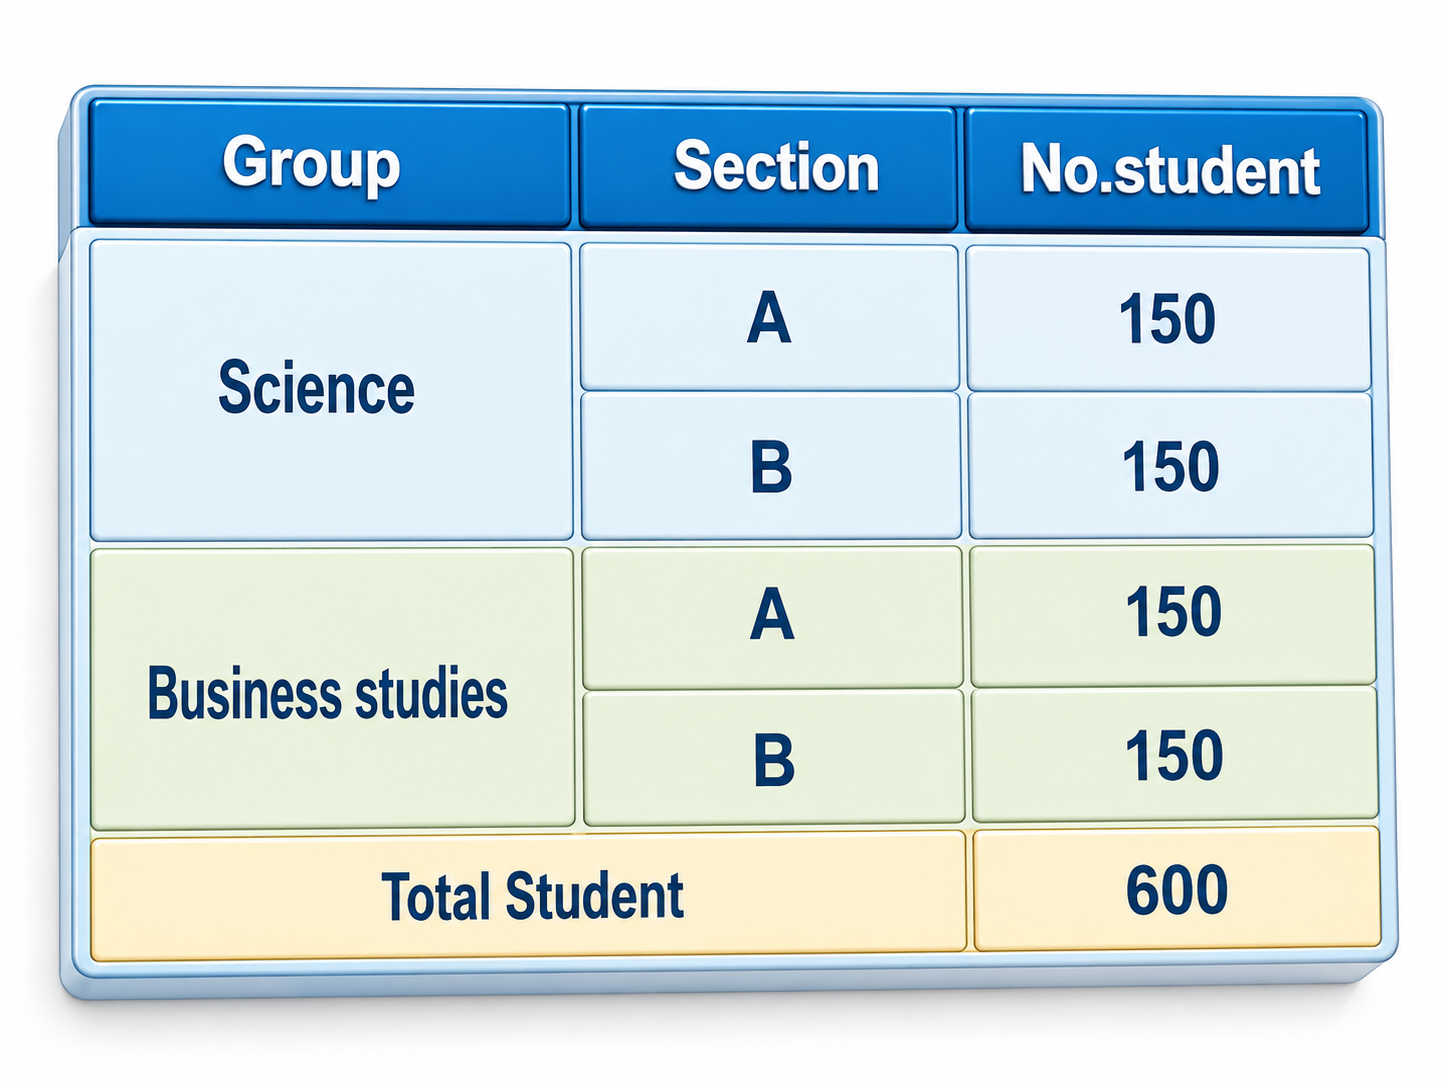
\includegraphics[width=0.95\linewidth,height=0.11\textheight,keepaspectratio]{chapters/Chapter04/topics/images/ex22_3d_group_section_student.png}
}{
\fbox{\parbox{0.90\linewidth}{\centering\vspace{0.45cm}
\textbf{চিত্র}\\[3pt]
File: \texttt{chapters/Chapter04/topics/images/ex22\_3d\_group\_section\_student.png}
\vspace{0.45cm}}}
}
\captionof{figure}{Group, Section and No. of student table}
\end{center}

\begin{keypointbox}{চিত্র ব্যাখ্যা}
Science এবং Business studies cell দুটি করে section row জুড়ে আছে। Total Student cell দুই column জুড়ে আছে।
\end{keypointbox}

\begin{keypointbox}{চিত্র দেখে code লেখার ধাপ}
প্রথমে figure-এর total row ও column গুনবে। এরপর কোন cell একাধিক column জুড়ে আছে তা দেখে \texttt{colspan} এবং কোন cell একাধিক row জুড়ে আছে তা দেখে \texttt{rowspan} বসাবে। তারপর image, link, list বা nested table থাকলে সংশ্লিষ্ট tag cell-এর ভিতরে লিখবে।
\end{keypointbox}

\par\noindent{\color{purple!70!black}\bfseries\small কোড}\par\vspace{-4pt}
\begin{verbatim}
<!DOCTYPE html>
<html>
<head>
  <title>HTML Table Example</title>
</head>
<body>
<table border="1" cellspacing="0">
<tr>
  <th>Group</th>
  <th>Section</th>
  <th>No. of student</th>
</tr>
<tr>
  <td rowspan="2">Science</td>
  <td>A</td>
  <td>150</td>
</tr>
<tr>
  <td>B</td>
  <td>150</td>
</tr>
<tr>
  <td rowspan="2">Business studies</td>
  <td>A</td>
  <td>150</td>
</tr>
<tr>
  <td>B</td>
  <td>150</td>
</tr>
<tr>
  <td colspan="2" align="center">Total student</td>
  <td>600</td>
</tr>
</table>
</body>
</html>
\end{verbatim}
\vspace{-6pt}

\subsubsection{Exercise 23: ID, Name and Contact No Table}

\begin{center}
\IfFileExists{chapters/Chapter04/topics/images/ex23_3d_contact_no_colspan.png}{
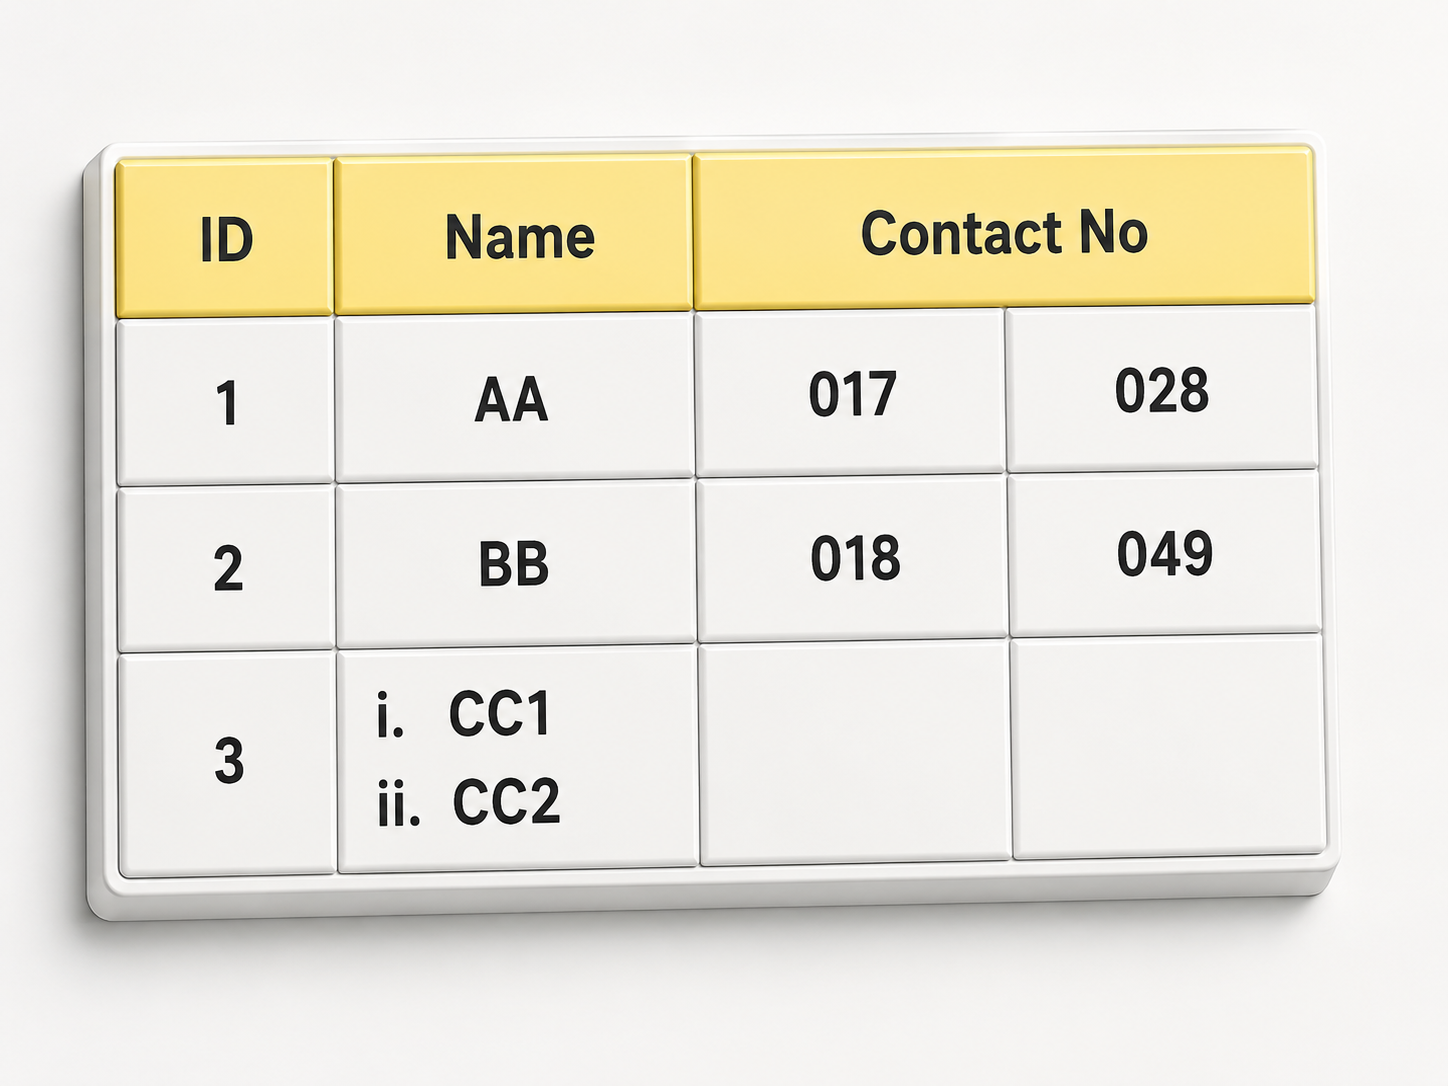
\includegraphics[width=0.95\linewidth,height=0.11\textheight,keepaspectratio]{chapters/Chapter04/topics/images/ex23_3d_contact_no_colspan.png}
}{
\fbox{\parbox{0.90\linewidth}{\centering\vspace{0.45cm}
\textbf{চিত্র}\\[3pt]
File: \texttt{chapters/Chapter04/topics/images/ex23\_3d\_contact\_no\_colspan.png}
\vspace{0.45cm}}}
}
\captionof{figure}{Contact No table with bgcolor and colspan}
\end{center}

\begin{keypointbox}{চিত্র ব্যাখ্যা}
Contact No heading দুই column জুড়ে আছে। Header row-তে yellow background color ব্যবহার করা হয়েছে। শেষ row-তে ordered list type i ব্যবহার করা হয়েছে।
\end{keypointbox}

\par\noindent{\color{purple!70!black}\bfseries\small কোড}\par\vspace{-4pt}
\begin{verbatim}
<!DOCTYPE html>
<html>
<head>
  <title>HTML Table Example</title>
</head>
<body>
<table border="1" cellspacing="0">
<tr bgcolor="yellow">
  <th>ID</th>
  <th>Name</th>
  <th colspan="2">Contact No</th>
</tr>
<tr>
  <td>1</td>
  <td>AA</td>
  <td>017</td>
  <td>028</td>
</tr>
<tr>
  <td>2</td>
  <td>BB</td>
  <td>018</td>
  <td>049</td>
</tr>
<tr>
  <td>3</td>
  <td>
    <ol type="i">
      <li>CC1</li>
      <li>CC2</li>
    </ol>
  </td>
  <td colspan="2"><br></td>
</tr>
</table>
</body>
</html>
\end{verbatim}
\vspace{-6pt}

\subsubsection{Exercise 24: Govt. Rajendra College Table with Image and Links}

\begin{center}
\IfFileExists{chapters/Chapter04/topics/images/ex24_3d_college_image_links.png}{
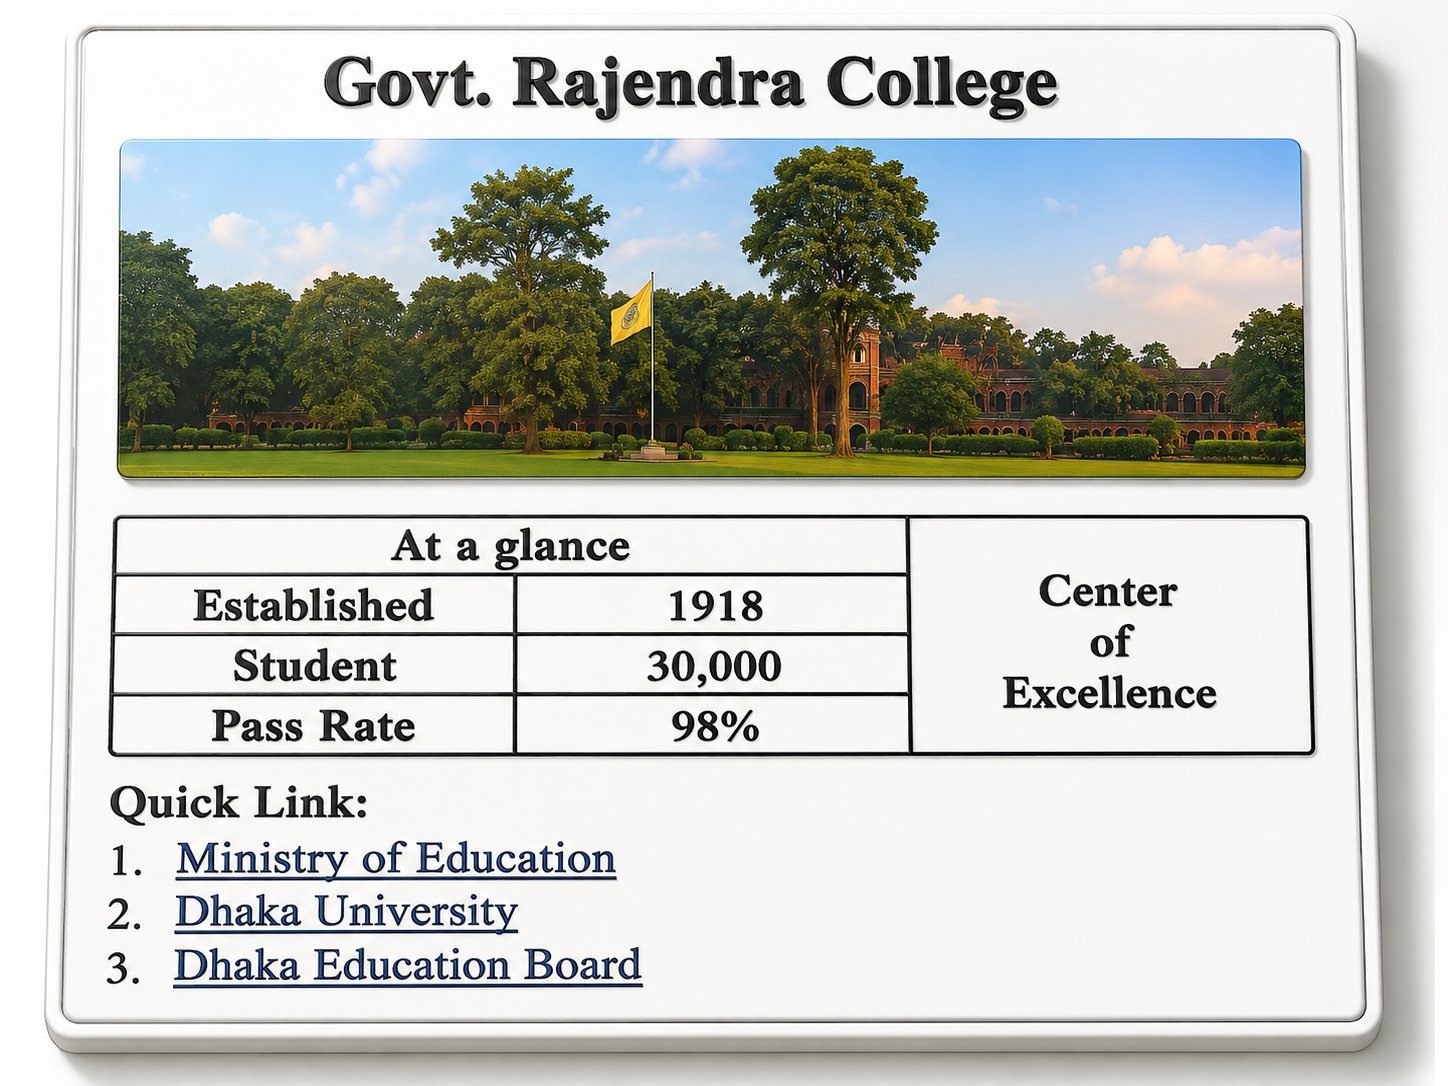
\includegraphics[width=0.95\linewidth,height=0.11\textheight,keepaspectratio]{chapters/Chapter04/topics/images/ex24_3d_college_image_links.png}
}{
\fbox{\parbox{0.90\linewidth}{\centering\vspace{0.45cm}
\textbf{চিত্র}\\[3pt]
File: \texttt{chapters/Chapter04/topics/images/ex24\_3d\_college\_image\_links.png}
\vspace{0.45cm}}}
}
\captionof{figure}{Govt. Rajendra College table with image, nested info and quick links}
\end{center}

\begin{keypointbox}{চিত্র ব্যাখ্যা}
এই example-এ heading, image, At a glance table এবং quick link একসাথে ব্যবহার করা হয়েছে। Center of Excellence cell চার row জুড়ে আছে।
\end{keypointbox}

\begin{keypointbox}{চিত্র দেখে code লেখার ধাপ}
প্রথমে figure-এর total row ও column গুনবে। এরপর কোন cell একাধিক column জুড়ে আছে তা দেখে \texttt{colspan} এবং কোন cell একাধিক row জুড়ে আছে তা দেখে \texttt{rowspan} বসাবে। তারপর image, link, list বা nested table থাকলে সংশ্লিষ্ট tag cell-এর ভিতরে লিখবে।
\end{keypointbox}

\par\noindent{\color{purple!70!black}\bfseries\small কোড}\par\vspace{-4pt}
\begin{verbatim}
<!DOCTYPE html>
<html>
<head>
  <title>HTML Table Example</title>
</head>
<body>
<h3 align="center">Govt. Rajendra College</h3>
<img src="college.jpg" width="400" height="200" align="center"><br>
<table border="1" cellspacing="0" align="center">
<tr>
  <th colspan="2">At a glance</th>
  <td rowspan="4" align="center">Center<br>of<br>Excellence</td>
</tr>
<tr>
  <th>Established</th>
  <td>1918</td>
</tr>
<tr>
  <th>Student</th>
  <td>30,000</td>
</tr>
<tr>
  <th>Pass Rate</th>
  <td>98%</td>
</tr>
</table>
<p>Quick Link:<br>
<a href="http://www.moedu.gov.bd">Ministry of Education</a><br>
<a href="www.du.ac.bd">Dhaka University</a><br>
<a href="www.dhakaeducationboard.gov.bd">Dhaka Education Board</a><br>
</p>
</body>
</html>
\end{verbatim}
\vspace{-6pt}

\subsubsection{Exercise 25: Department Male/Female Table with Photo}

\begin{center}
\IfFileExists{chapters/Chapter04/topics/images/ex25_3d_department_photo.png}{
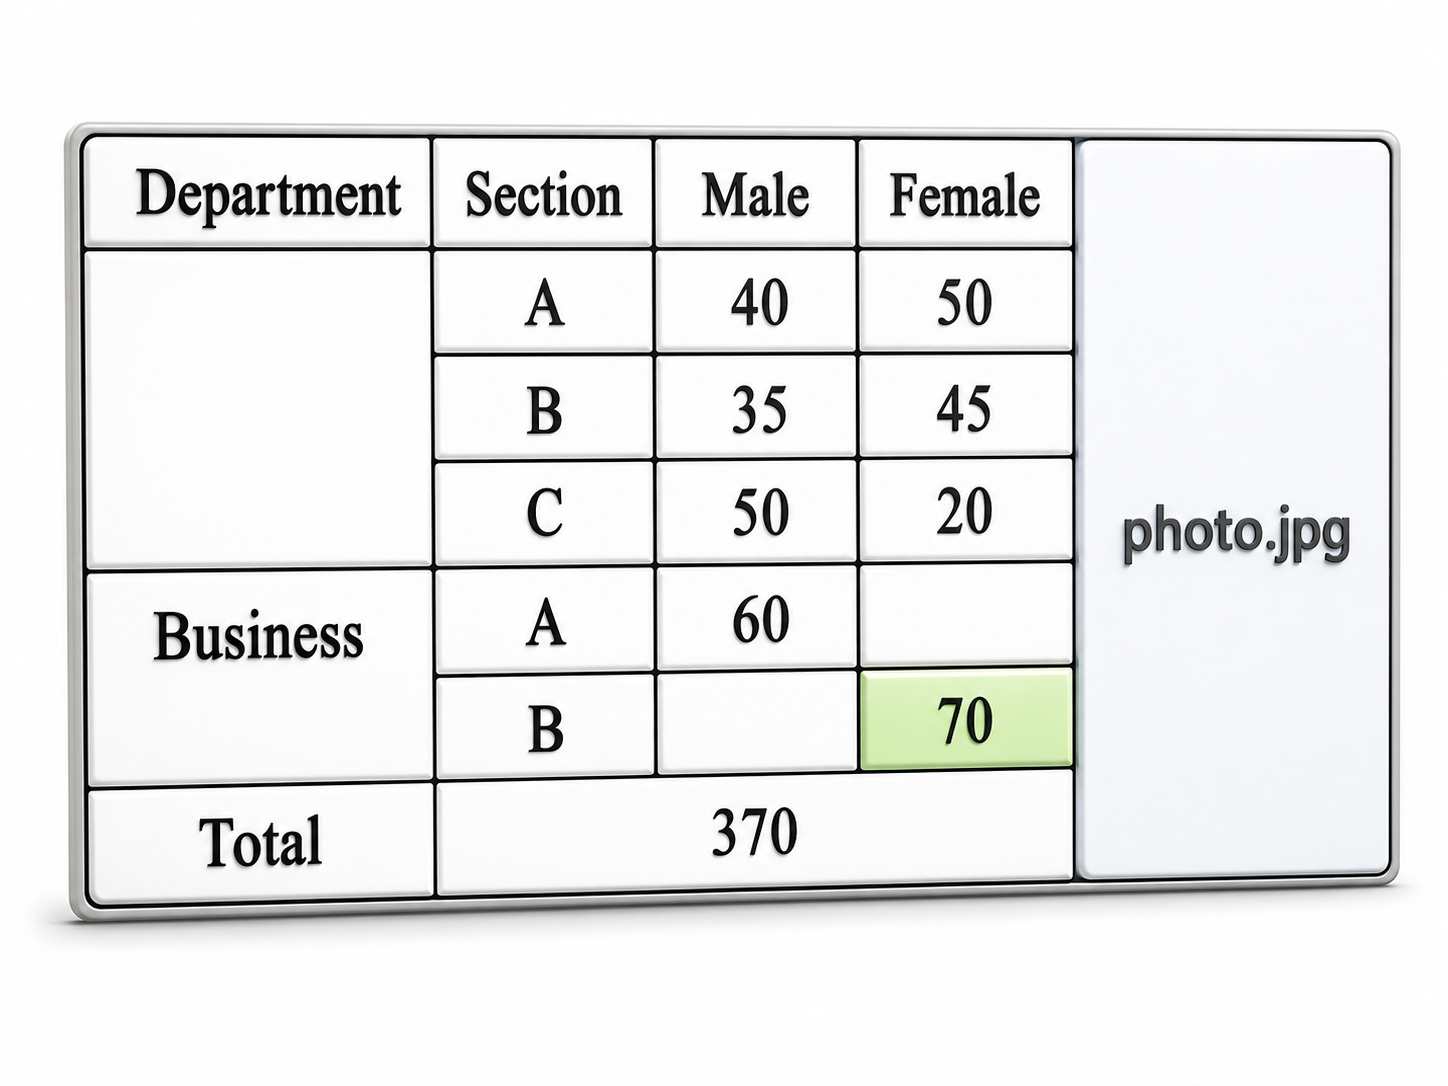
\includegraphics[width=0.95\linewidth,height=0.11\textheight,keepaspectratio]{chapters/Chapter04/topics/images/ex25_3d_department_photo.png}
}{
\fbox{\parbox{0.90\linewidth}{\centering\vspace{0.45cm}
\textbf{চিত্র}\\[3pt]
File: \texttt{chapters/Chapter04/topics/images/ex25\_3d\_department\_photo.png}
\vspace{0.45cm}}}
}
\captionof{figure}{Department table with photo, rowspan, total and green cell}
\end{center}

\begin{keypointbox}{চিত্র ব্যাখ্যা}
Photo column সাত row জুড়ে আছে। Business cell দুই row জুড়ে আছে। 70 cell-এর background green। Total row-তে total text ও 370 value center aligned করে দেখানো হয়েছে।
\end{keypointbox}

\par\noindent{\color{purple!70!black}\bfseries\small কোড}\par\vspace{-4pt}
\begin{verbatim}
<!DOCTYPE html>
<html>
<head>
  <title>HTML Table Example</title>
</head>
<body>
  <table border="1" cellspacing="0">
    <tr>
      <th>Department</th><th>Section</th><th>Male</th><th>Female</th>
      <th rowspan="7"><img src="photo.jpg" width="60" height="50" alt="Photo"></th>
    </tr>
    <tr><td rowspan="3">&nbsp;</td><td>A</td><td>40</td><td>50</td></tr>
    <tr><td>B</td><td>35</td><td>45</td></tr>
    <tr><td>C</td><td>50</td><td>20</td></tr>
    <tr><td rowspan="2" align="center">Business</td><td>A</td><td>60</td><td>&nbsp;</td></tr>
    <tr><td>B</td><td>&nbsp;</td><td bgcolor="green">70</td></tr>
    <tr><td align="center">Total</td><td colspan="3" align="center">370</td></tr>
  </table>
</body>
</html>
\end{verbatim}
\vspace{-6pt}

\Needspace{10\baselineskip}
\subsubsection{Exercise 26: Science, Commerce and Humanities Table}

\begin{boardbox}{Concept}
Group-wise subject table-এ first column group দেখায় এবং বাকি columnগুলো subject list দেখায়। চিত্র দেখে row ও column count ঠিক করা সবচেয়ে জরুরি।
\end{boardbox}

\begin{center}
\IfFileExists{chapters/Chapter04/topics/images/ex26_3d_group_subjects.png}{
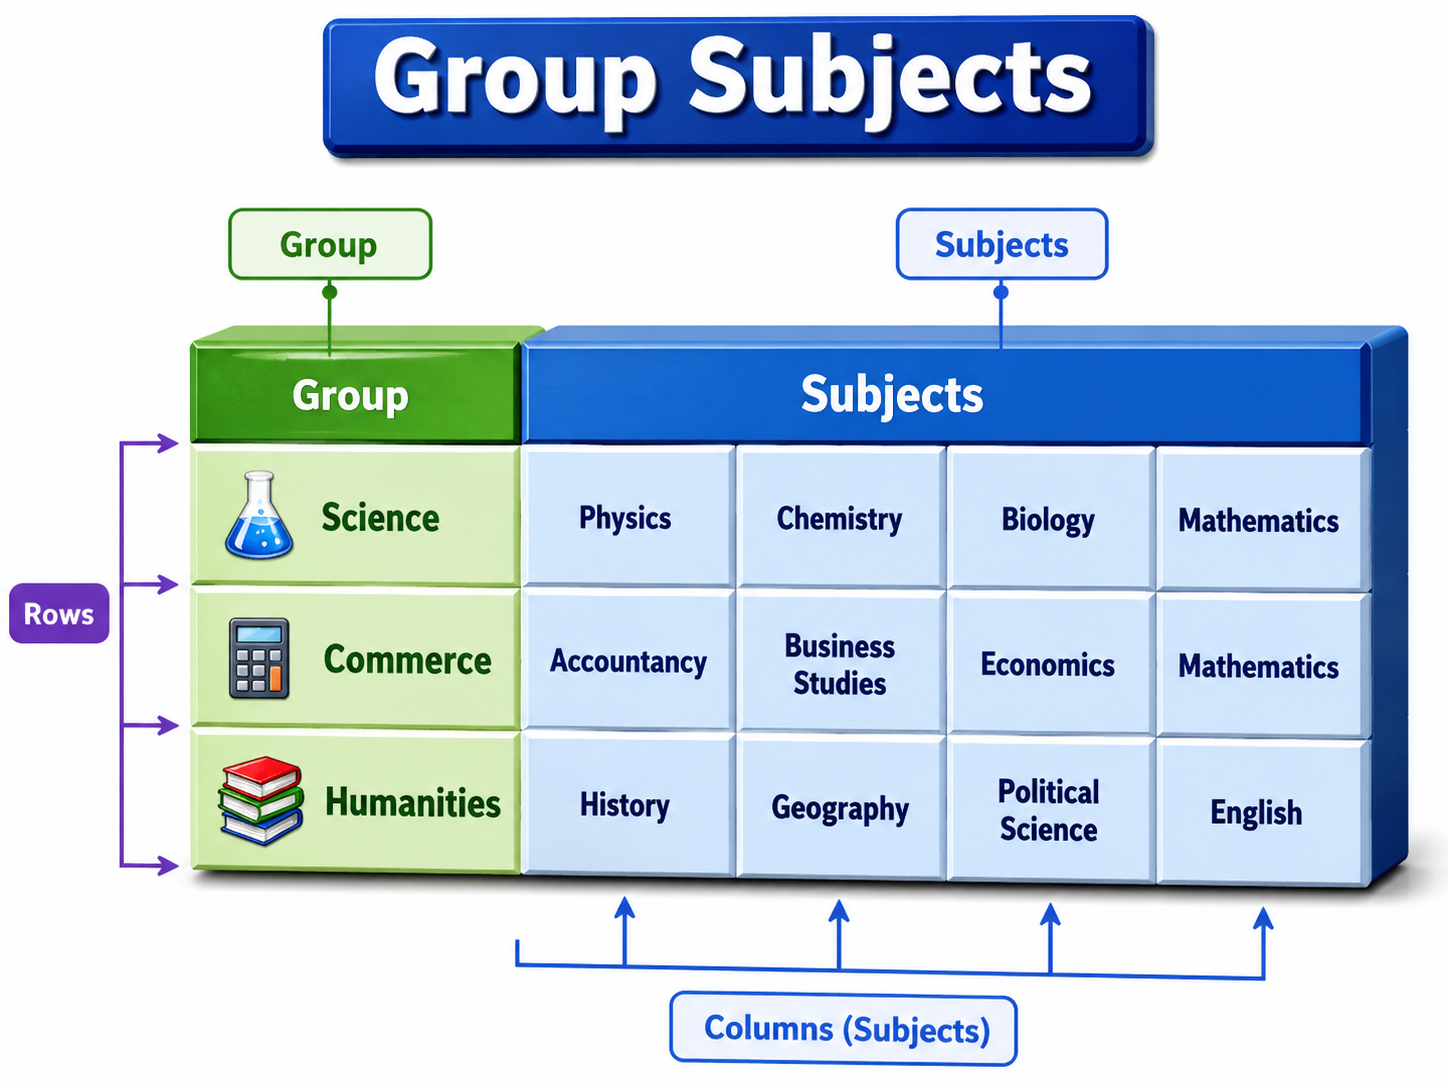
\includegraphics[width=0.95\linewidth,height=0.11\textheight,keepaspectratio]{chapters/Chapter04/topics/images/ex26_3d_group_subjects.png}
}{
\fbox{\parbox{0.90\linewidth}{\centering\vspace{0.4cm}
\textbf{চিত্র}\\
File: \texttt{chapters/Chapter04/topics/images/ex26\_3d\_group\_subjects.png}
\vspace{0.4cm}}}
}
\captionof{figure}{Exercise 26-এর subject group চিত্র}
\end{center}

\begin{keypointbox}{চিত্র ব্যাখ্যা}
চিত্রে Group Subjects নামে একটি table আছে। প্রথম column-এ Science, Commerce ও Humanities group দেখানো হয়েছে। প্রতিটি group row-তে Physics/Chemistry/Biology/Mathematics, Accountancy/Business Studies/Economics/Mathematics এবং History/Geography/Political Science/English subject দেওয়া আছে।
\end{keypointbox}

\begin{keypointbox}{চিত্র দেখে code লেখার ধাপ}
প্রথমে title row-তে \texttt{colspan="5"} ব্যবহার করবে, কারণ table-এ Group সহ মোট 5টি column আছে। দ্বিতীয় row-তে Group ও Subjects heading লিখবে; Subjects heading চারটি subject column জুড়ে থাকবে। এরপর তিনটি group row লিখবে।
\end{keypointbox}

\par\noindent{\color{purple!70!black}\bfseries\small কোড}\par\vspace{-4pt}
\begin{verbatim}
<!DOCTYPE html>
<html>
<head>
  <title>HTML Table Example</title>
</head>
<body>
<table border="1" cellspacing="0" cellpadding="6" align="center">
  <tr>
    <th colspan="5">Group Subjects</th>
  </tr>
  <tr>
    <th>Group</th>
    <th colspan="4">Subjects</th>
  </tr>
  <tr>
    <td>Science</td>
    <td>Physics</td>
    <td>Chemistry</td>
    <td>Biology</td>
    <td>Mathematics</td>
  </tr>
  <tr>
    <td>Commerce</td>
    <td>Accountancy</td>
    <td>Business Studies</td>
    <td>Economics</td>
    <td>Mathematics</td>
  </tr>
  <tr>
    <td>Humanities</td>
    <td>History</td>
    <td>Geography</td>
    <td>Political Science</td>
    <td>English</td>
  </tr>
</table>
</body>
</html>
\end{verbatim}
\vspace{-6pt}
\subsubsection{Exercise 27: List Inside Table Cell}

\begin{center}
\IfFileExists{chapters/Chapter04/topics/images/ex27_3d_lists_inside_table.png}{
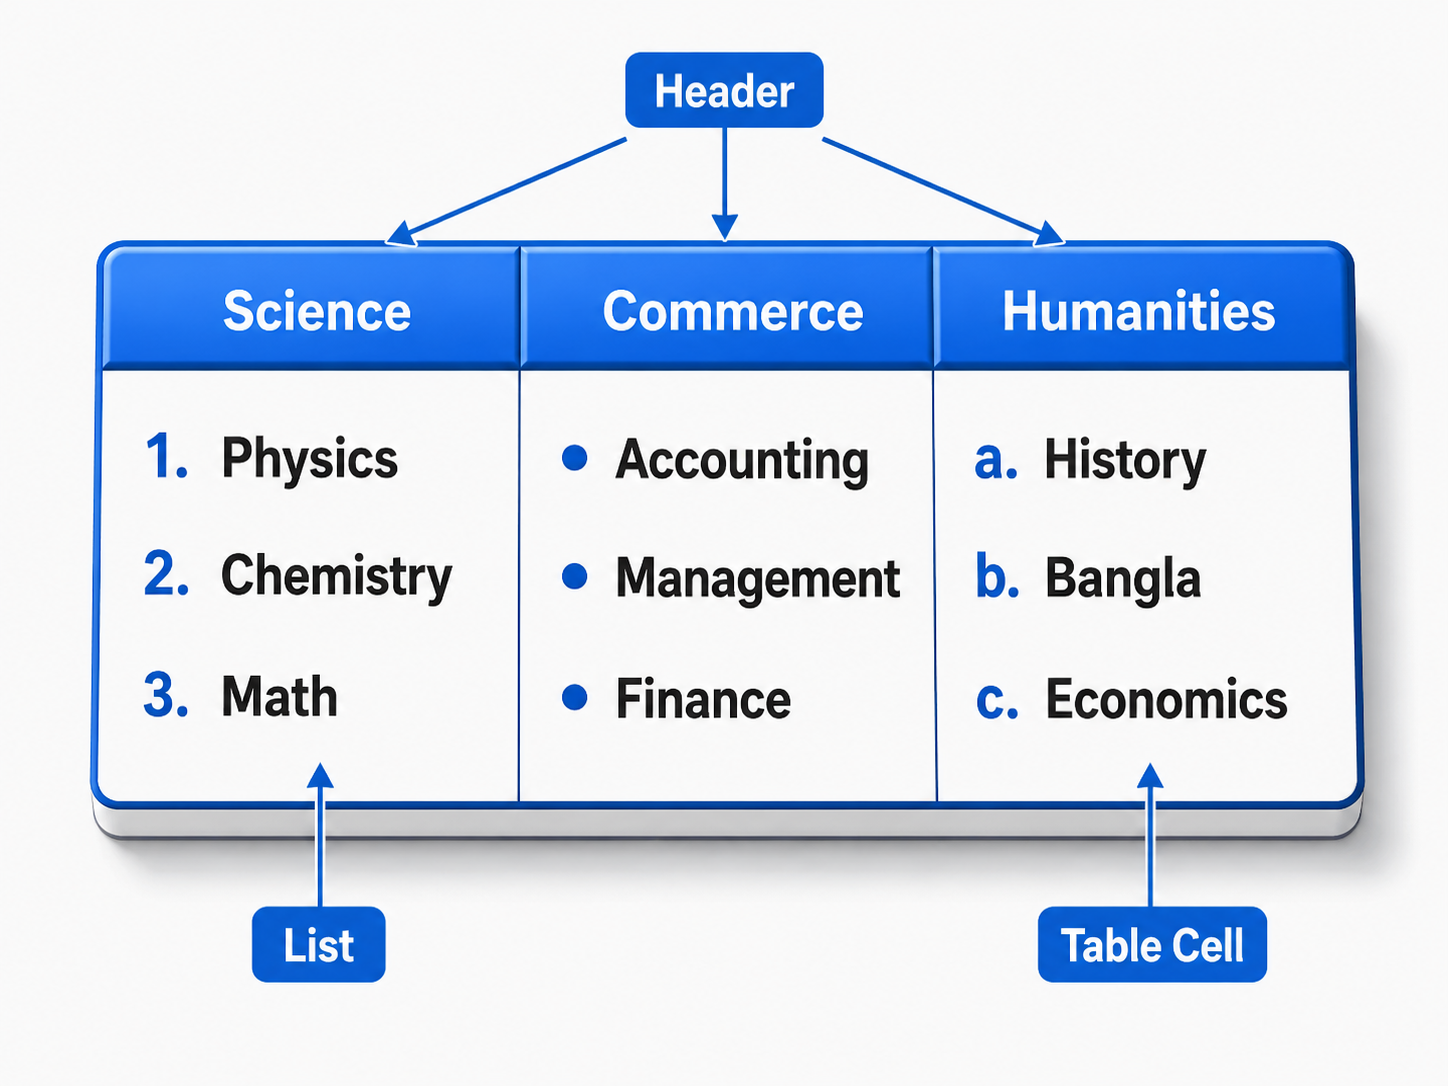
\includegraphics[width=0.95\linewidth,height=0.11\textheight,keepaspectratio]{chapters/Chapter04/topics/images/ex27_3d_lists_inside_table.png}
}{
\fbox{\parbox{0.90\linewidth}{\centering\vspace{0.45cm}
\textbf{চিত্র}\\[3pt]
File: \texttt{chapters/Chapter04/topics/images/ex27\_3d\_lists\_inside\_table.png}
\vspace{0.45cm}}}
}
\captionof{figure}{List inside table cell: Science, Commerce ও Humanities}
\end{center}

\begin{keypointbox}{চিত্র ব্যাখ্যা}
এই table-এ তিনটি column আছে: Science, Commerce ও Humanities। প্রতিটি cell-এর ভিতরে আলাদা type-এর list ব্যবহার করা হয়েছে: ordered list, unordered list এবং alphabetic ordered list।
\end{keypointbox}

\begin{keypointbox}{চিত্র দেখে code লেখার ধাপ}
প্রথমে figure-এর total row ও column গুনবে। এরপর কোন cell একাধিক column জুড়ে আছে তা দেখে \texttt{colspan} এবং কোন cell একাধিক row জুড়ে আছে তা দেখে \texttt{rowspan} বসাবে। তারপর image, link, list বা nested table থাকলে সংশ্লিষ্ট tag cell-এর ভিতরে লিখবে।
\end{keypointbox}

\par\noindent{\color{purple!70!black}\bfseries\small কোড}\par\vspace{-4pt}
\begin{verbatim}
<!DOCTYPE html>
<html>
<head>
  <title>HTML Table Example</title>
</head>
<body>
<table border="1" cellspacing="0">
<tr>
  <th>Science</th>
  <th>Commerce</th>
  <th>Humanities</th>
</tr>
<tr>
  <td><ol><li>Physics</li><li>Chemistry</li><li>Math</li></ol></td>
  <td><ul><li>Accounting</li><li>Management</li><li>Finance</li></ul></td>
  <td><ol type="a"><li>History</li><li>Bangla</li><li>Economics</li></ol></td>
</tr>
</table>
</body>
</html>
\end{verbatim}
\vspace{-6pt}

\subsubsection{Exercise 28: Teacher Information Table with Picture}

\begin{center}
\IfFileExists{chapters/Chapter04/topics/images/ex28_3d_teacher_info_picture.png}{
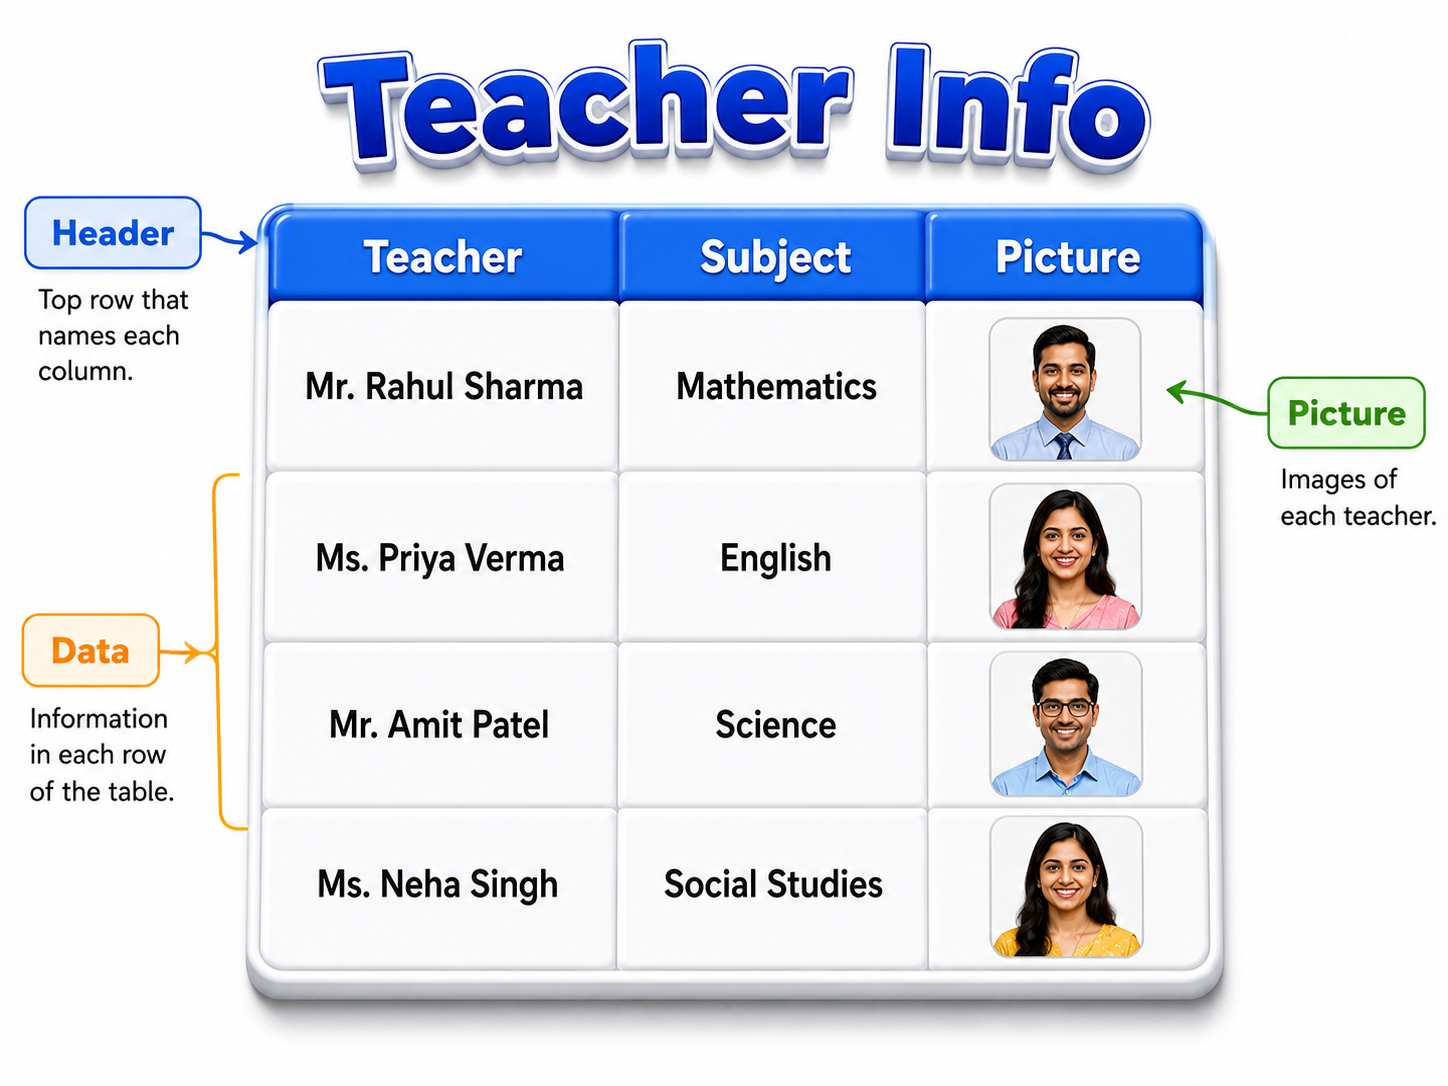
\includegraphics[width=0.95\linewidth,height=0.11\textheight,keepaspectratio]{chapters/Chapter04/topics/images/ex28_3d_teacher_info_picture.png}
}{
\fbox{\parbox{0.90\linewidth}{\centering\vspace{0.45cm}
\textbf{চিত্র}\\[3pt]
File: \texttt{chapters/Chapter04/topics/images/ex28\_3d\_teacher\_info\_picture.png}
\vspace{0.45cm}}}
}
\captionof{figure}{Teacher Info table with subject and picture column}
\end{center}

\begin{keypointbox}{চিত্র ব্যাখ্যা}
চিত্রে Teacher Info heading আছে এবং table-এ Teacher, Subject ও Picture--এই তিনটি column দেখা যায়। প্রতিটি row-তে teacher name, subject এবং সংশ্লিষ্ট picture রাখা হয়েছে।
\end{keypointbox}

\begin{keypointbox}{চিত্র দেখে code লেখার ধাপ}
প্রথমে title/heading আলাদা করবে। তারপর তিনটি column--Teacher, Subject, Picture--লিখবে। Picture column-এর প্রতিটি cell-এ \texttt{<img>} tag বসাবে এবং image size নির্ধারণ করবে।
\end{keypointbox}

\par\noindent{\color{purple!70!black}\bfseries\small কোড}\par\vspace{-4pt}
\begin{verbatim}
<!DOCTYPE html>
<html>
<head>
  <title>HTML Table Example</title>
</head>
<body>
<h2 align="center">Teacher Info</h2>
<table border="1" align="center" cellspacing="0" cellpadding="6">
<tr>
  <th>Teacher</th>
  <th>Subject</th>
  <th>Picture</th>
</tr>
<tr>
  <td>Mr. Rahul Sharma</td>
  <td>Mathematics</td>
  <td><img src="rahul.jpg" width="55" height="60" alt="Rahul Sharma"></td>
</tr>
<tr>
  <td>Mrs. Priya Verma</td>
  <td>English</td>
  <td><img src="priya.jpg" width="55" height="60" alt="Priya Verma"></td>
</tr>
<tr>
  <td>Mr. Amit Patel</td>
  <td>Science</td>
  <td><img src="amit.jpg" width="55" height="60" alt="Amit Patel"></td>
</tr>
<tr>
  <td>Ms. Neha Singh</td>
  <td>Social Studies</td>
  <td><img src="neha.jpg" width="55" height="60" alt="Neha Singh"></td>
</tr>
</table>
</body>
</html>
\end{verbatim}
\vspace{-6pt}

\subsubsection{Exercise 29: Bangladesh Places Table with Photo}

\begin{center}
\IfFileExists{chapters/Chapter04/topics/images/ex29_3d_bangladesh_places.png}{
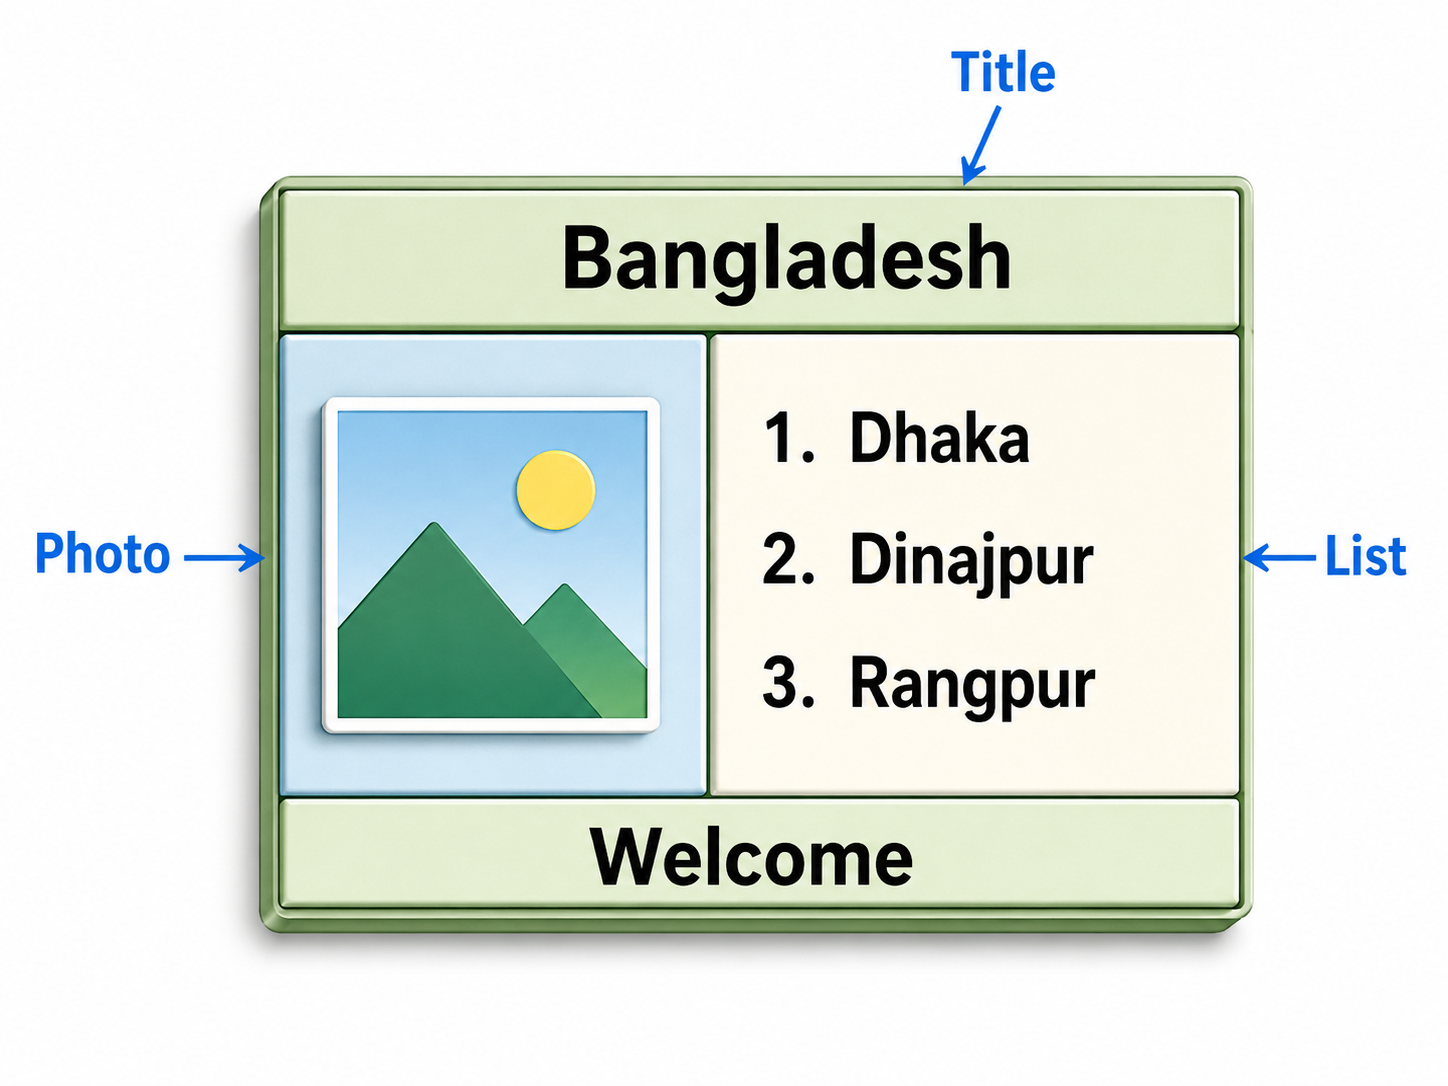
\includegraphics[width=0.95\linewidth,height=0.11\textheight,keepaspectratio]{chapters/Chapter04/topics/images/ex29_3d_bangladesh_places.png}
}{
\fbox{\parbox{0.90\linewidth}{\centering\vspace{0.45cm}
\textbf{চিত্র}\\[3pt]
File: \texttt{chapters/Chapter04/topics/images/ex29\_3d\_bangladesh\_places.png}
\vspace{0.45cm}}}
}
\captionof{figure}{Bangladesh table with photo and ordered list}
\end{center}

\begin{keypointbox}{চিত্র ব্যাখ্যা}
এই table-এ top heading এবং bottom welcome row দুটি column জুড়ে আছে। মাঝের row-তে বাম cell-এ image এবং ডান cell-এ ordered list রাখা হয়েছে।
\end{keypointbox}

\begin{keypointbox}{চিত্র দেখে code লেখার ধাপ}
প্রথমে figure-এর total row ও column গুনবে। এরপর কোন cell একাধিক column জুড়ে আছে তা দেখে \texttt{colspan} এবং কোন cell একাধিক row জুড়ে আছে তা দেখে \texttt{rowspan} বসাবে। তারপর image, link, list বা nested table থাকলে সংশ্লিষ্ট tag cell-এর ভিতরে লিখবে।
\end{keypointbox}

\par\noindent{\color{purple!70!black}\bfseries\small কোড}\par\vspace{-4pt}
\begin{verbatim}
<!DOCTYPE html>
<html>
<head>
  <title>HTML Table Example</title>
</head>
<body>
<table border="1" cellspacing="0">
<tr><th colspan="2">Bangladesh</th></tr>
<tr>
  <td><img src="photo.jpg" width="60" height="50" align="center"><br>Photo</td>
  <td>
    <ol>
      <li>Dhaka</li>
      <li>Dinajpur</li>
      <li>Rangpur</li>
    </ol>
  </td>
</tr>
<tr><th colspan="2">Welcome</th></tr>
</table>
</body>
</html>
\end{verbatim}
\vspace{-6pt}

\subsubsection{Exercise 30: Choose Your Site Table with Links}

\begin{center}
\IfFileExists{chapters/Chapter04/topics/images/ex30_3d_choose_site_links.png}{
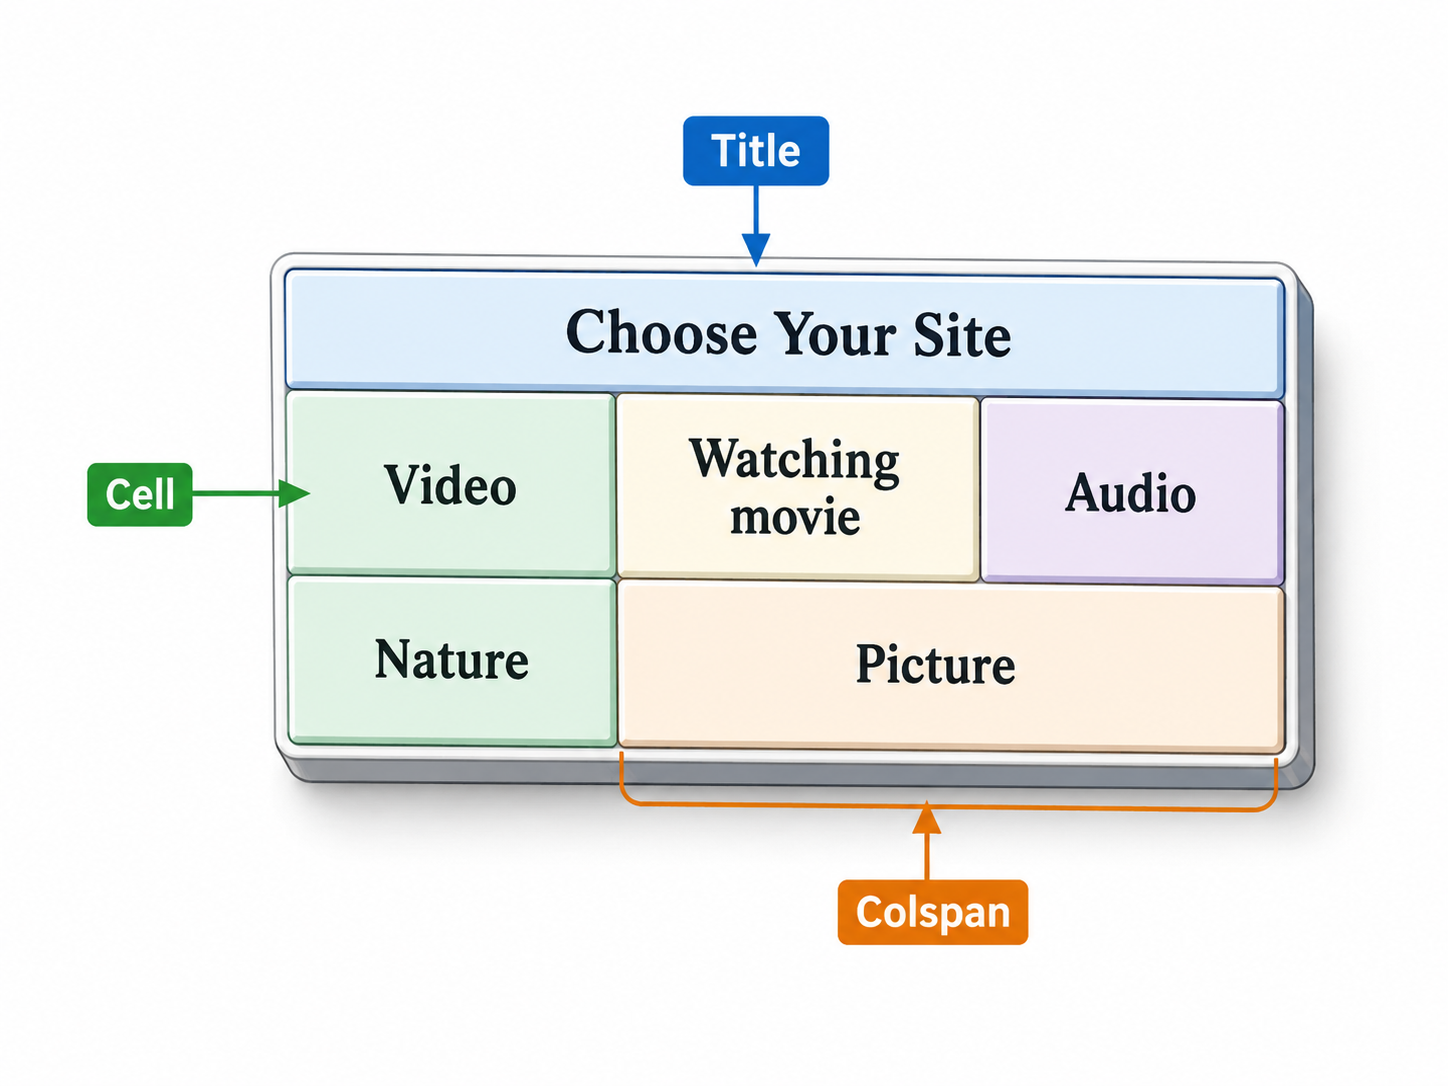
\includegraphics[width=0.95\linewidth,height=0.11\textheight,keepaspectratio]{chapters/Chapter04/topics/images/ex30_3d_choose_site_links.png}
}{
\fbox{\parbox{0.90\linewidth}{\centering\vspace{0.45cm}
\textbf{চিত্র}\\[3pt]
File: \texttt{chapters/Chapter04/topics/images/ex30\_3d\_choose\_site\_links.png}
\vspace{0.45cm}}}
}
\captionof{figure}{Choose Your Site table with centered and underlined text}
\end{center}

\begin{keypointbox}{চিত্র ব্যাখ্যা}
এখানে \texttt{colspan="3"} দিয়ে title row তিনটি column জুড়ে আছে। Video ও Nature underline করা হয়েছে এবং Picture cell দুই column জুড়ে আছে।
\end{keypointbox}

\par\noindent{\color{purple!70!black}\bfseries\small কোড}\par\vspace{-4pt}
\begin{verbatim}
<!DOCTYPE html>
<html>
<head>
  <title>HTML Table Example</title>
</head>
<body>
<table border="1" cellspacing="0">
<tr>
  <th colspan="3">Choose Your Site</th>
</tr>
<tr>
  <td align="center"><u>Video</u><br></td>
  <td>Watching<br><p align="center">movie</p></td>
  <td>Audio</td>
</tr>
<tr>
  <td align="center"><u>Nature</u></td>
  <td colspan="2" align="center"><br>Picture</td>
</tr>
</table>
</body>
</html>
\end{verbatim}
\vspace{-6pt}

\subsubsection{Exercise 31: XY Showroom Table}

\begin{center}
\IfFileExists{chapters/Chapter04/topics/images/ex31_3d_xy_showroom.png}{
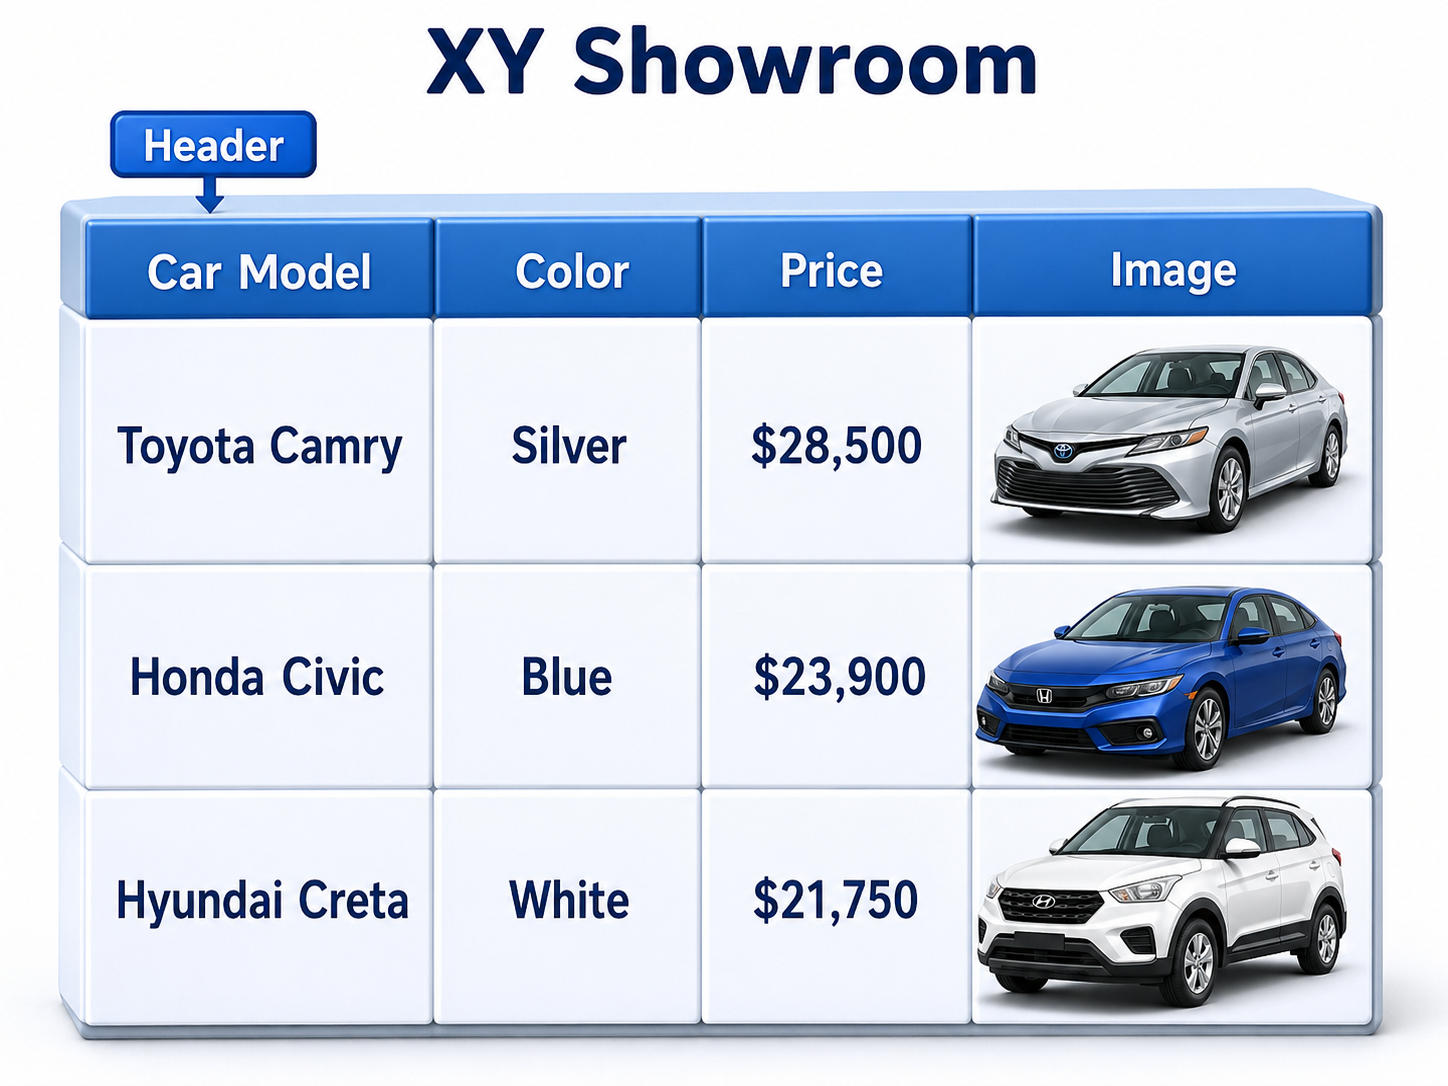
\includegraphics[width=0.95\linewidth,height=0.11\textheight,keepaspectratio]{chapters/Chapter04/topics/images/ex31_3d_xy_showroom.png}
}{
\fbox{\parbox{0.90\linewidth}{\centering\vspace{0.45cm}
\textbf{চিত্র}\\[3pt]
File: \texttt{chapters/Chapter04/topics/images/ex31\_3d\_xy\_showroom.png}
\vspace{0.45cm}}}
}
\captionof{figure}{XY Showroom table with car model, color, price and image}
\end{center}

\begin{keypointbox}{চিত্র ব্যাখ্যা}
চিত্রে XY Showroom heading-এর নিচে Car Model, Color, Price এবং Image--চারটি column আছে। প্রতিটি car row-তে model, color, price এবং car image দেখানো হয়েছে।
\end{keypointbox}

\begin{keypointbox}{চিত্র দেখে code লেখার ধাপ}
প্রথমে table-এর উপরে \texttt{<h2>} heading লিখবে। তারপর চারটি header cell তৈরি করবে। প্রতিটি row-তে car model, color, price এবং image cell লিখবে। Image column-এ \texttt{<img>} tag ব্যবহার করবে।
\end{keypointbox}

\par\noindent{\color{purple!70!black}\bfseries\small কোড}\par\vspace{-4pt}
\begin{verbatim}
<!DOCTYPE html>
<html>
<head>
  <title>XY Showroom</title>
</head>
<body>
<h2 align="center">XY Showroom</h2>
<table border="1" align="center" cellspacing="0" cellpadding="6">
<tr>
  <th>Car Model</th>
  <th>Color</th>
  <th>Price</th>
  <th>Image</th>
</tr>
<tr>
  <td>Toyota Camry</td>
  <td>Silver</td>
  <td>$28,500</td>
  <td><img src="camry.jpg" width="100" height="60" alt="Toyota Camry"></td>
</tr>
<tr>
  <td>Honda Civic</td>
  <td>Blue</td>
  <td>$23,900</td>
  <td><img src="civic.jpg" width="100" height="60" alt="Honda Civic"></td>
</tr>
<tr>
  <td>Hyundai Creta</td>
  <td>White</td>
  <td>$21,750</td>
  <td><img src="creta.jpg" width="100" height="60" alt="Hyundai Creta"></td>
</tr>
</table>
</body>
</html>
\end{verbatim}
\vspace{-6pt}

\subsubsection{Exercise 32: Nested Table Example}

\begin{center}
\IfFileExists{chapters/Chapter04/topics/images/ex32_3d_nested_table_parent_child.png}{
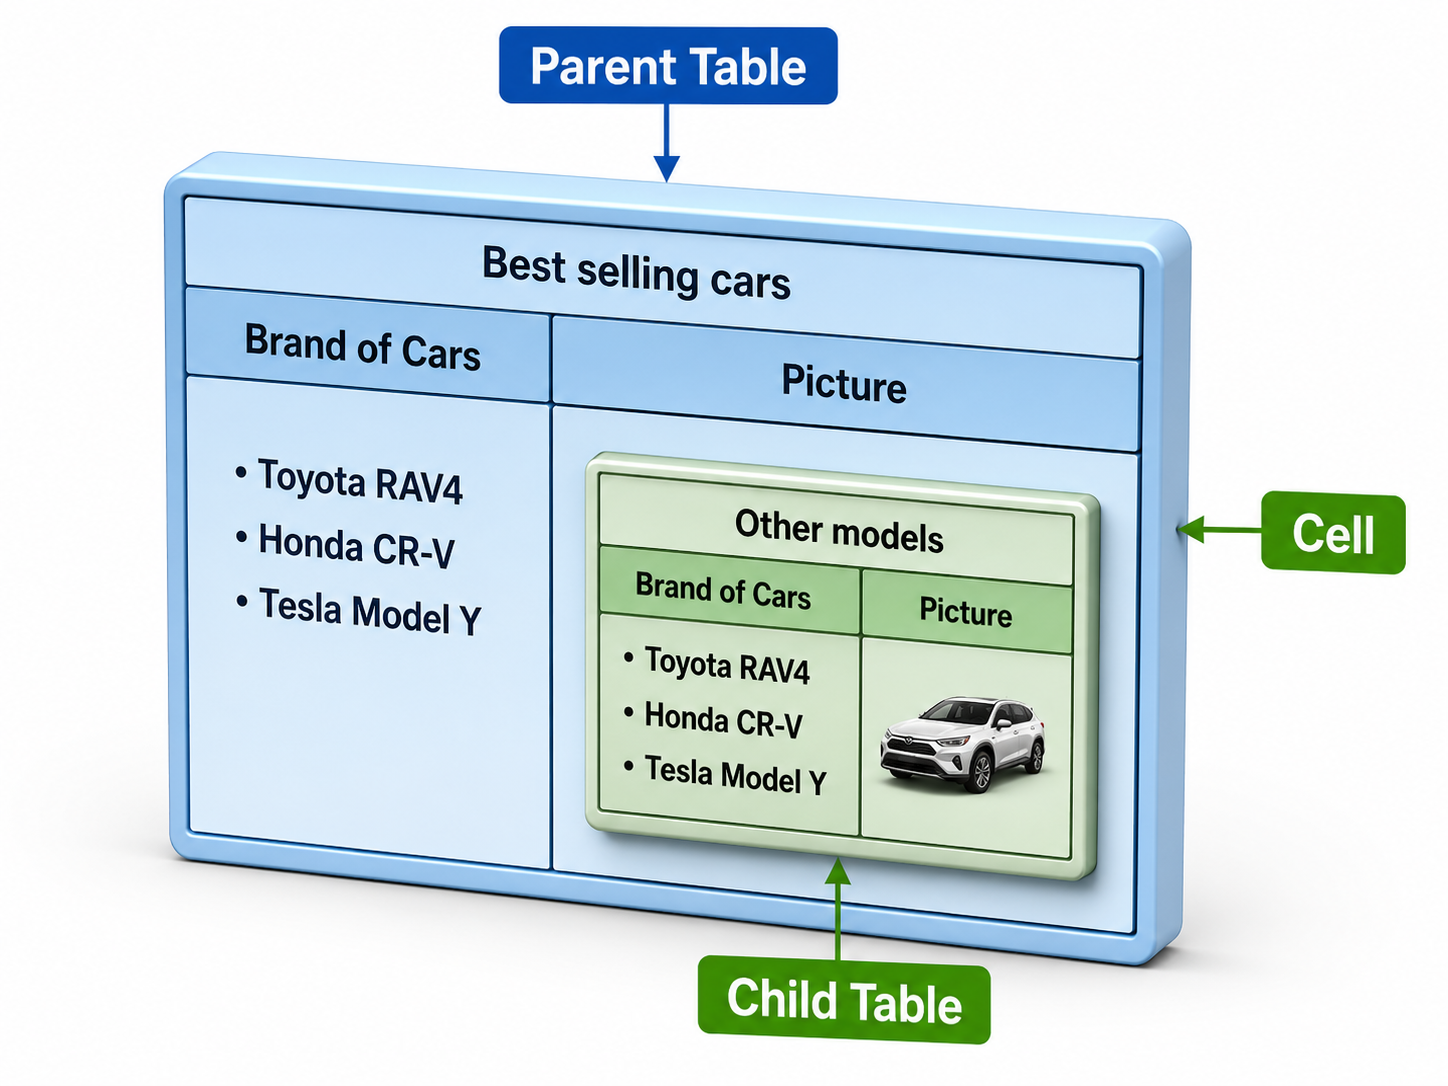
\includegraphics[width=0.95\linewidth,height=0.11\textheight,keepaspectratio]{chapters/Chapter04/topics/images/ex32_3d_nested_table_parent_child.png}
}{
\fbox{\parbox{0.90\linewidth}{\centering\vspace{0.45cm}
\textbf{চিত্র}\\[3pt]
File: \texttt{chapters/Chapter04/topics/images/ex32\_3d\_nested\_table\_parent\_child.png}
\vspace{0.45cm}}}
}
\captionof{figure}{Nested table: parent table-এর cell-এর ভিতরে child table}
\end{center}

\begin{keypointbox}{চিত্র ব্যাখ্যা}
Nested table-এ একটি বড় parent table-এর কোনো একটি cell-এর ভিতরে আরেকটি ছোট child table বসানো হয়। বইয়ের example-এ বিস্তারিত অংশের ভিতরে ছোট table ব্যবহার করা হয়েছে।
\end{keypointbox}

\begin{keypointbox}{চিত্র দেখে code লেখার ধাপ}
প্রথমে figure-এর total row ও column গুনবে। এরপর কোন cell একাধিক column জুড়ে আছে তা দেখে \texttt{colspan} এবং কোন cell একাধিক row জুড়ে আছে তা দেখে \texttt{rowspan} বসাবে। তারপর image, link, list বা nested table থাকলে সংশ্লিষ্ট tag cell-এর ভিতরে লিখবে।
\end{keypointbox}

\par\noindent{\color{purple!70!black}\bfseries\small কোড}\par\vspace{-4pt}
\begin{verbatim}
<!DOCTYPE html>
<html>
<head>
  <title>Table Inside Table</title>
</head>
<body>
<h3>বাইরের টেবিল (Parent Table)</h3>
<table border="2" cellpadding="10">
<tr>
  <th>নাম</th>
  <th>বিস্তারিত</th>
</tr>
<tr>
  <td>রাফি</td>
  <td>
    <!-- ভিতরের টেবিল শুরু -->
    <table border="1" cellpadding="5">
    <tr>
      <th>বিষয়</th>
      <th>নম্বর</th>
    </tr>
    <tr>
      <td>গণিত</td>
      <td>৮৫</td>
    </tr>
    <tr>
      <td>বিজ্ঞান</td>
      <td>৯০</td>
    </tr>
    </table>
    <!-- ভিতরের টেবিল শেষ -->
  </td>
</tr>
</table>
</body>
</html>
\end{verbatim}
\vspace{-6pt}

\subsubsection{Exercise 33: Student Subjects Table}

\begin{center}
\IfFileExists{chapters/Chapter04/topics/images/ex33_3d_student_subjects.png}{
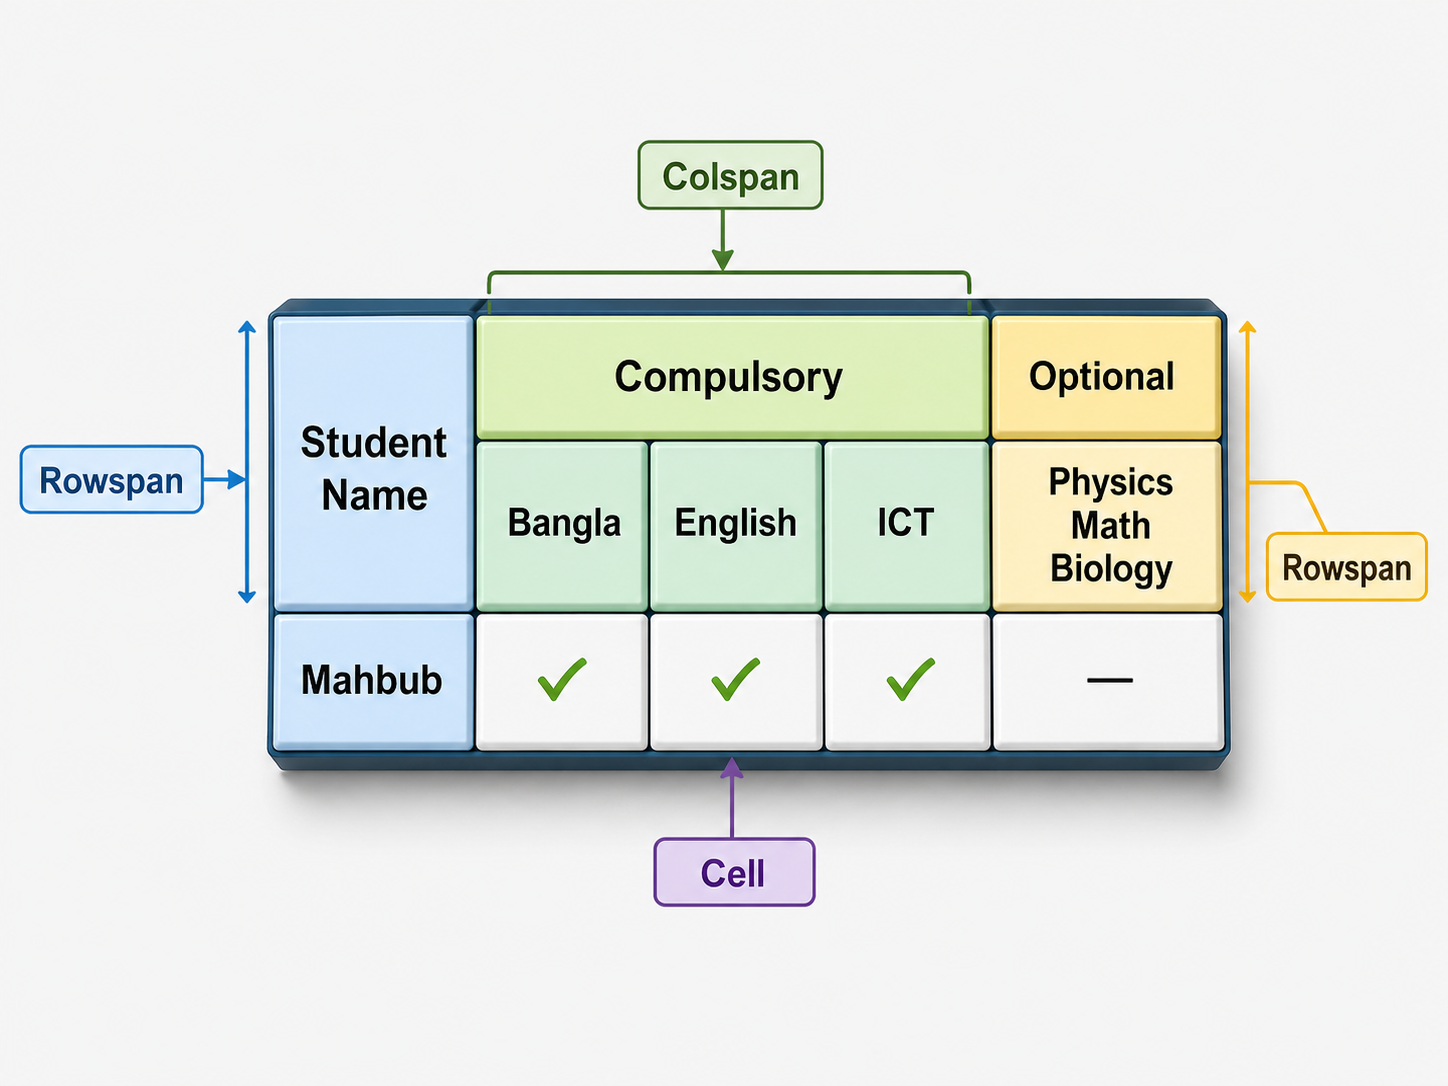
\includegraphics[width=0.95\linewidth,height=0.11\textheight,keepaspectratio]{chapters/Chapter04/topics/images/ex33_3d_student_subjects.png}
}{
\fbox{\parbox{0.90\linewidth}{\centering\vspace{0.45cm}
\textbf{চিত্র}\\[3pt]
File: \texttt{chapters/Chapter04/topics/images/ex33\_3d\_student\_subjects.png}
\vspace{0.45cm}}}
}
\captionof{figure}{Student Subjects table with rowspan and colspan}
\end{center}

\begin{keypointbox}{চিত্র ব্যাখ্যা}
Student Name এবং Optional heading দুই row জুড়ে আছে। Compulsory heading তিনটি subject column জুড়ে আছে। Mahbub ও tick mark cell-গুলো তিনটি optional subject row জুড়ে আছে।
\end{keypointbox}

\par\noindent{\color{purple!70!black}\bfseries\small কোড}\par\vspace{-4pt}
\begin{verbatim}
<!DOCTYPE html>
<html>
<head>
  <title>Student Subjects Table</title>
</head>
<body>
<table border="1" cellspacing="0">
<tr>
  <th rowspan="2">Student Name</th>
  <th colspan="3">Compulsory</th>
  <th rowspan="2">Optional</th>
</tr>
<tr>
  <td>Bangla</td>
  <td>English</td>
  <td>ICT</td>
</tr>
<tr>
  <th rowspan="3">Mahbub</th>
  <th rowspan="3">&#10003;</th>
  <th rowspan="3">&#10003;</th>
  <th rowspan="3">&#10003;</th>
  <td>Physics</td>
</tr>
<tr><td>Math</td></tr>
<tr><td>Biology</td></tr>
</table>
</body>
</html>
\end{verbatim}
\vspace{-6pt}

\subsubsection{Exercise 34: Science Fair Projects Table}

\begin{center}
\IfFileExists{chapters/Chapter04/topics/images/ex34_3d_science_fair_projects.png}{
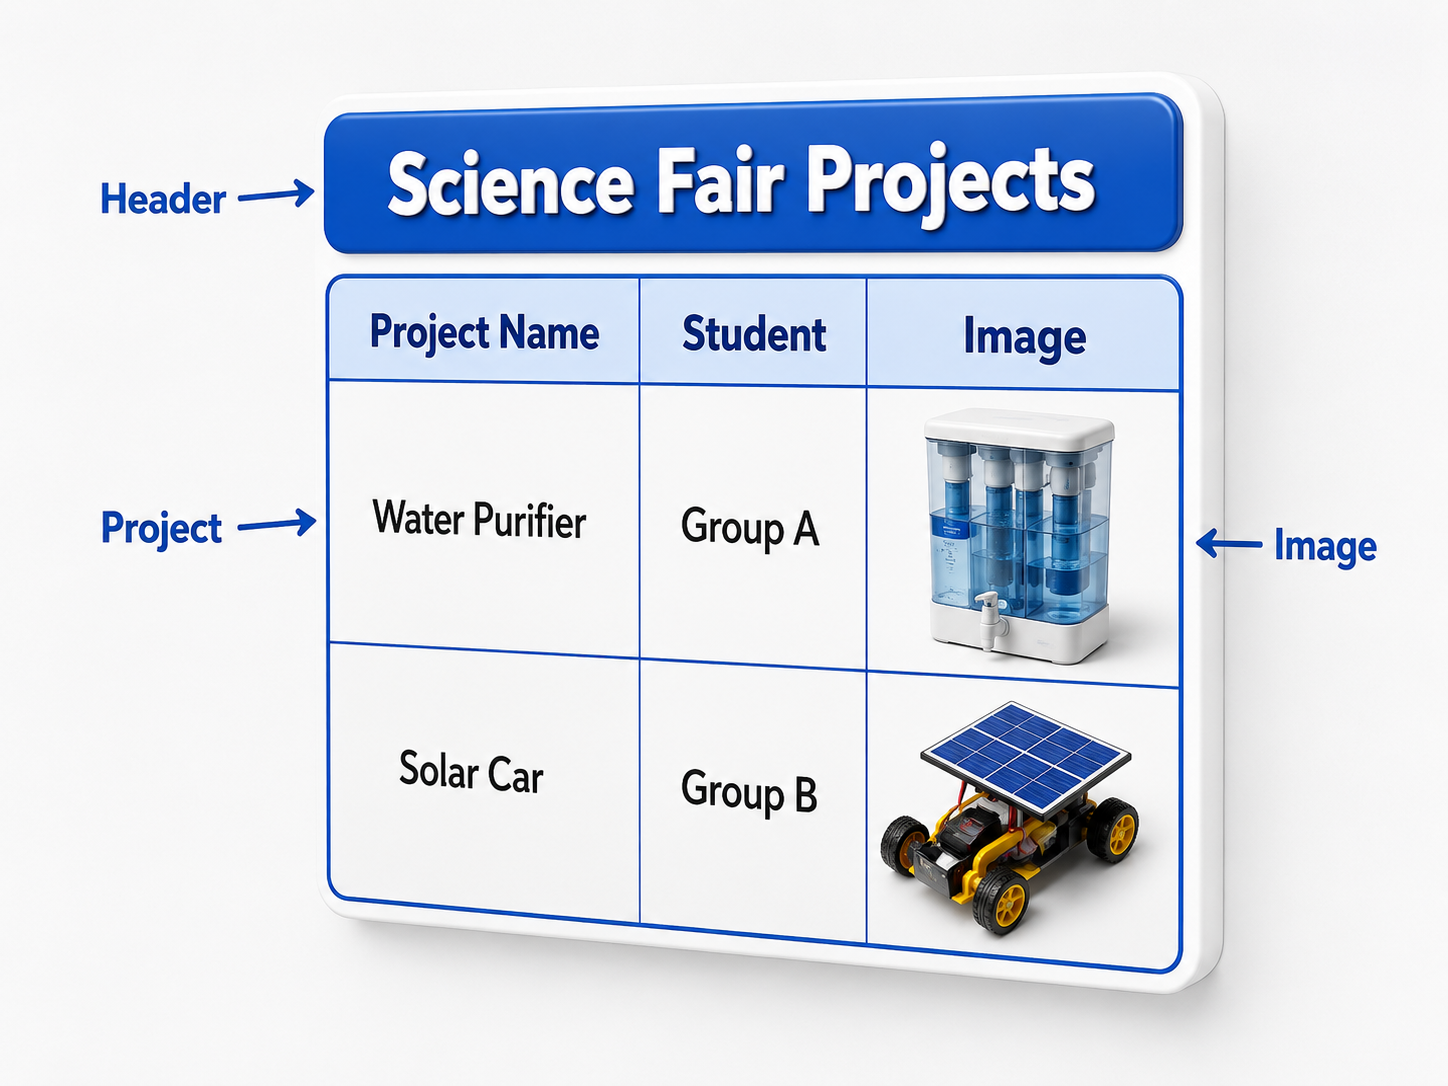
\includegraphics[width=0.95\linewidth,height=0.11\textheight,keepaspectratio]{chapters/Chapter04/topics/images/ex34_3d_science_fair_projects.png}
}{
\fbox{\parbox{0.90\linewidth}{\centering\vspace{0.45cm}
\textbf{চিত্র}\\[3pt]
File: \texttt{chapters/Chapter04/topics/images/ex34\_3d\_science\_fair\_projects.png}
\vspace{0.45cm}}}
}
\captionof{figure}{Science Fair Projects table with student/group and image}
\end{center}

\begin{keypointbox}{চিত্র ব্যাখ্যা}
চিত্রে Science Fair Projects heading-এর নিচে Project Name, Student এবং Image column আছে। প্রতিটি project row-তে project name, group/student label এবং project image দেওয়া হয়েছে।
\end{keypointbox}

\begin{keypointbox}{চিত্র দেখে code লেখার ধাপ}
প্রথমে heading লিখবে। এরপর তিনটি column identify করবে: Project Name, Student এবং Image। শেষ column-এ প্রতিটি project-এর জন্য \texttt{<img>} tag বসাবে।
\end{keypointbox}

\par\noindent{\color{purple!70!black}\bfseries\small কোড}\par\vspace{-4pt}
\begin{verbatim}
<!DOCTYPE html>
<html>
<head>
  <title>HTML Table Example</title>
</head>
<body>
<h2 align="center">Science Fair Projects</h2>
<table border="1" align="center" cellspacing="0" cellpadding="6">
<tr>
  <th>Project Name</th>
  <th>Student</th>
  <th>Image</th>
</tr>
<tr>
  <td>Water Purifier</td>
  <td>Group A</td>
  <td><img src="purifier.jpg" width="80" height="60" alt="Water Purifier"></td>
</tr>
<tr>
  <td>Solar Car</td>
  <td>Group B</td>
  <td><img src="solarcar.jpg" width="80" height="60" alt="Solar Car"></td>
</tr>
</table>
</body>
</html>
\end{verbatim}
\vspace{-6pt}

\subsubsection{Exercise 35: Group, Section and Club Table}

\begin{center}
\IfFileExists{chapters/Chapter04/topics/images/ex35_3d_group_section_club.png}{
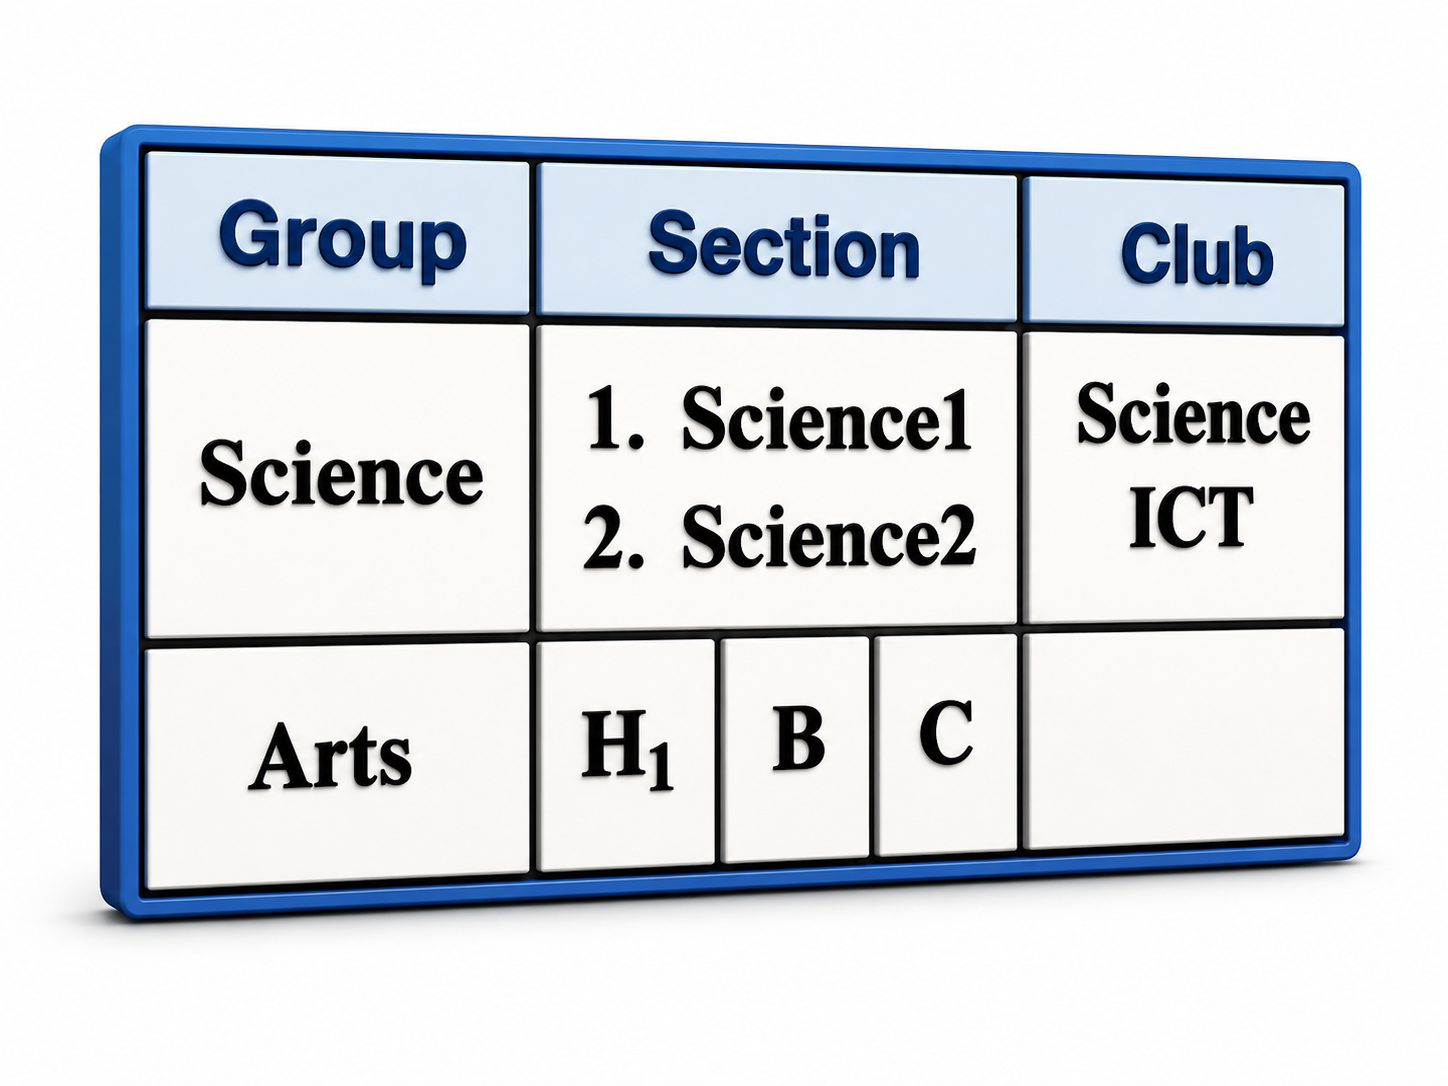
\includegraphics[width=0.95\linewidth,height=0.11\textheight,keepaspectratio]{chapters/Chapter04/topics/images/ex35_3d_group_section_club.png}
}{
\fbox{\parbox{0.90\linewidth}{\centering\vspace{0.45cm}
\textbf{চিত্র}\\[3pt]
File: \texttt{chapters/Chapter04/topics/images/ex35\_3d\_group\_section\_club.png}
\vspace{0.45cm}}}
}
\captionof{figure}{Group, Section and Club table with colspan, rowspan, sub and span}
\end{center}

\begin{keypointbox}{চিত্র ব্যাখ্যা}
Section heading তিনটি column জুড়ে আছে। Club cell দুই row জুড়ে আছে। Science row-তে Section অংশ তিনটি column জুড়ে text দেখানো হয়েছে। Arts row-তে H\textsubscript{1}, B এবং C আলাদা cell-এ আছে।
\end{keypointbox}

\begin{keypointbox}{চিত্র দেখে code লেখার ধাপ}
প্রথমে figure-এর total row ও column গুনবে। এরপর কোন cell একাধিক column জুড়ে আছে তা দেখে \texttt{colspan} এবং কোন cell একাধিক row জুড়ে আছে তা দেখে \texttt{rowspan} বসাবে। তারপর image, link, list বা nested table থাকলে সংশ্লিষ্ট tag cell-এর ভিতরে লিখবে।
\end{keypointbox}

\par\noindent{\color{purple!70!black}\bfseries\small কোড}\par\vspace{-4pt}
\begin{verbatim}
<!DOCTYPE html>
<html>
<head>
  <title>Group Table</title>
</head>
<body>
<table border="1" cellspacing="0" cellpadding="5">
<tr>
  <th>Group</th>
  <th colspan="3">Section</th>
  <th rowspan="2"><u>Club</u><br>
    <span style="font-weight:normal;">Science<br>ICT</span>
  </th>
</tr>
<tr>
  <td>Science</td>
  <td colspan="3">1. Science1<br>2. Science2</td>
</tr>
<tr>
  <td>Arts</td>
  <td>H<sub>1</sub></td>
  <td>B</td>
  <td>C</td>
  <td></td>
</tr>
</table>
</body>
</html>
\end{verbatim}
\vspace{-6pt}

\subsubsection{Exercise 36: Delight Restaurant Table}

\begin{center}
\IfFileExists{chapters/Chapter04/topics/images/ex36_3d_delight_restaurant.png}{
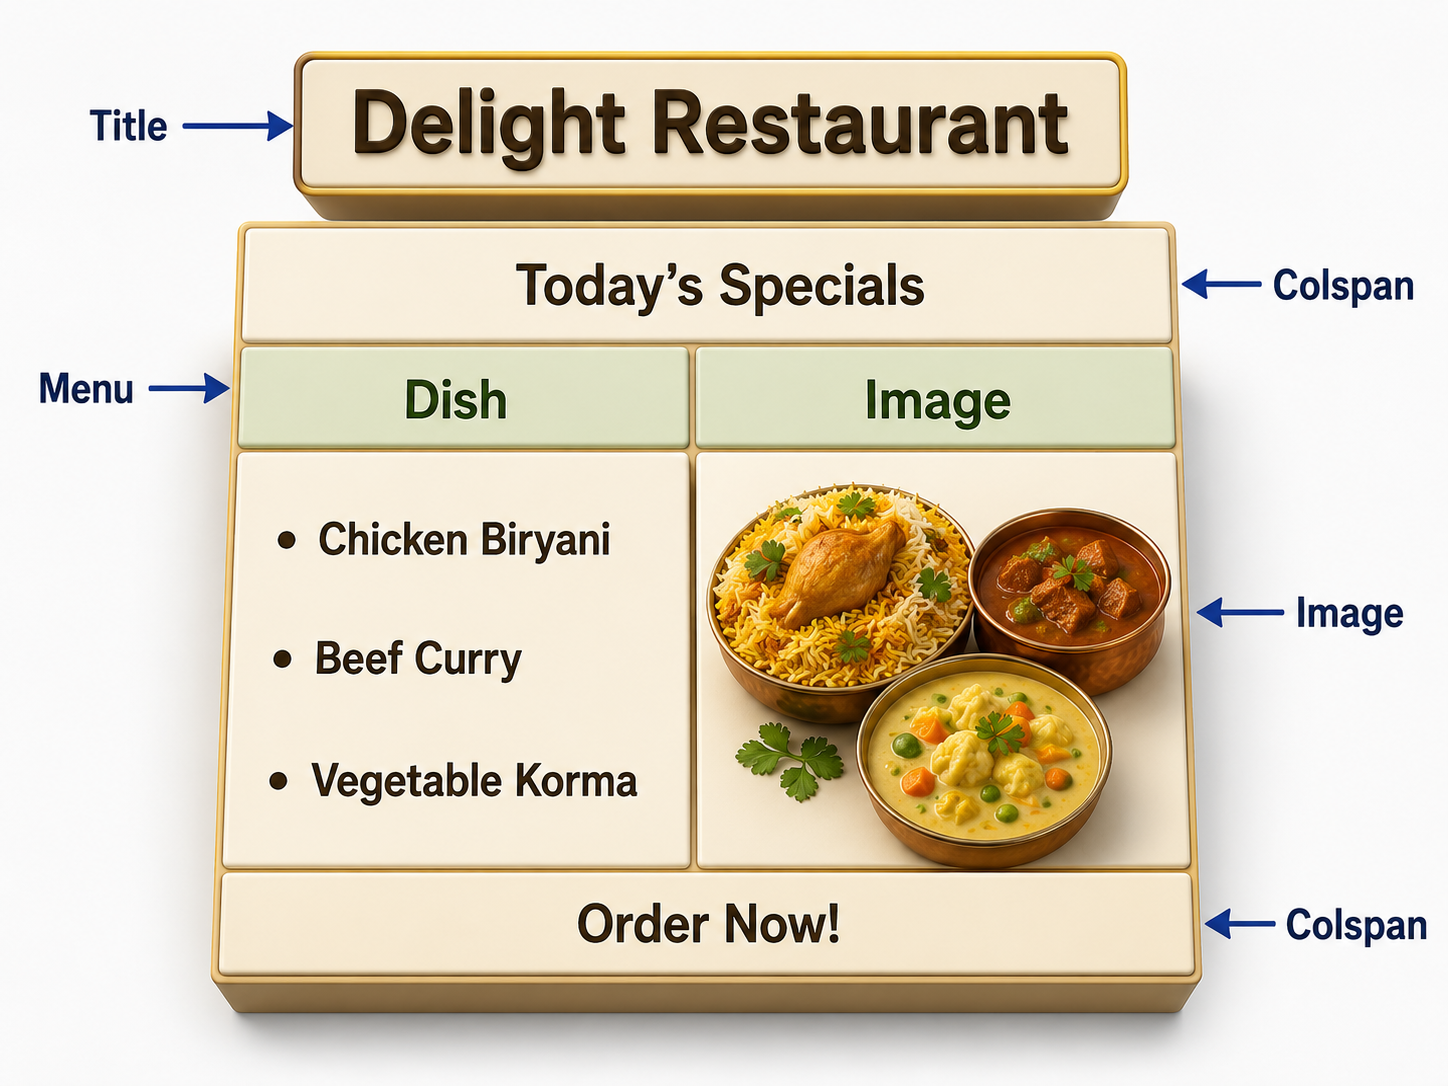
\includegraphics[width=0.95\linewidth,height=0.11\textheight,keepaspectratio]{chapters/Chapter04/topics/images/ex36_3d_delight_restaurant.png}
}{
\fbox{\parbox{0.90\linewidth}{\centering\vspace{0.45cm}
\textbf{চিত্র}\\[3pt]
File: \texttt{chapters/Chapter04/topics/images/ex36\_3d\_delight\_restaurant.png}
\vspace{0.45cm}}}
}
\captionof{figure}{Delight Restaurant table with food image and order row}
\end{center}

\begin{keypointbox}{চিত্র ব্যাখ্যা}
এই table-এ Today's Specials এবং Order Now row দুই column জুড়ে আছে। Dish cell-এ line break দিয়ে item list দেখানো হয়েছে এবং Image cell-এ food image রাখা হয়েছে।
\end{keypointbox}

\par\noindent{\color{purple!70!black}\bfseries\small কোড}\par\vspace{-4pt}
\begin{verbatim}
<!DOCTYPE html>
<html>
<head>
  <title>HTML Table Example</title>
</head>
<body>
<h2 align="center">Delight Restaurant</h2>
<table border="1" align="center" cellspacing="0" cellpadding="8">
<tr>
  <th colspan="2">Today's Specials</th>
</tr>
<tr>
  <th>Dish</th>
  <th>Image</th>
</tr>
<tr>
  <td>• Chicken Biryani<br>• Beef Curry<br>• Vegetable Korma</td>
  <td><img src="food.jpg" width="100" height="80" alt="Food"></td>
</tr>
<tr>
  <td colspan="2" align="center">Order Now!</td>
</tr>
</table>
</body>
</html>
\end{verbatim}
\vspace{-6pt}

% =========================================================
% Extra HSC ICT Board-Style Mixed HTML Table Examples
% Add this file after the main Table in HTML topic.
% Image labels should be short English labels; explanation remains in Bangla.
% =========================================================

\subsection{আরও Board-Style Mixed HTML Table Practice}

\begin{boardbox}{কেন এই অংশ গুরুত্বপূর্ণ}
HSC ICT practical/CQ-তে HTML table থেকে সাধারণত চিত্র দেখে code লিখতে বলা হয়। এসব প্রশ্নে \texttt{rowspan}, \texttt{colspan}, \texttt{image}, \texttt{hyperlink}, \texttt{list}, nested table, alignment ইত্যাদি মিশ্রভাবে থাকতে পারে। নিচের উদাহরণগুলো board-style practice হিসেবে তৈরি করা হয়েছে।
\end{boardbox}


\subsubsection{Example 55: Admission Schedule with Logo, Link, Rowspan and Colspan}

\begin{center}
\IfFileExists{chapters/Chapter04/topics/images/board_ex55_3d_admission_schedule.png}{
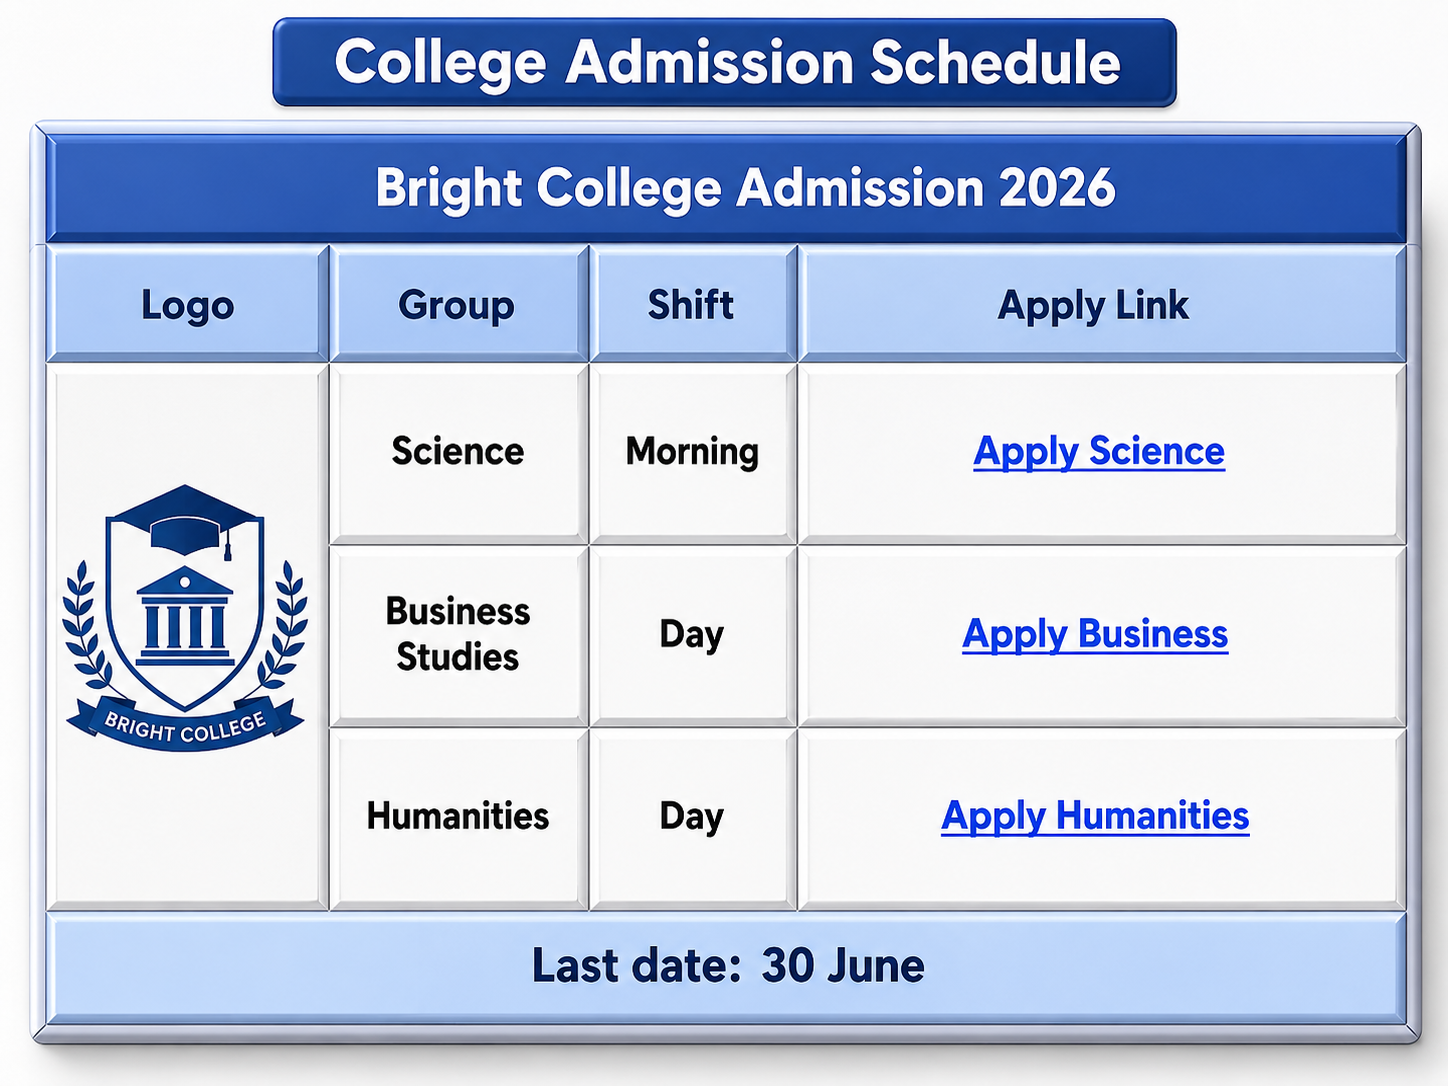
\includegraphics[width=0.95\linewidth,height=0.11\textheight,keepaspectratio]{chapters/Chapter04/topics/images/board_ex55_3d_admission_schedule.png}
}{
\fbox{\parbox{0.90\linewidth}{\centering\vspace{0.45cm}
\textbf{চিত্র}\\[3pt]
File: \texttt{chapters/Chapter04/topics/images/board\_ex55\_3d\_admission\_schedule.png}
\vspace{0.45cm}}}
}
\captionof{figure}{Admission Schedule with Logo, Link, Rowspan and Colspan}
\end{center}

\begin{keypointbox}{চিত্র ব্যাখ্যা}
এই example-এ logo image-এর জন্য rowspan, Apply Link অংশে colspan এবং শেষ row-তে full-width notice ব্যবহার করা হয়েছে।
\end{keypointbox}

\begin{keypointbox}{চিত্র দেখে code লেখার ধাপ}
প্রথমে figure-এর total row ও column গুনবে। এরপর কোন cell একাধিক column জুড়ে আছে তা দেখে \texttt{colspan} এবং কোন cell একাধিক row জুড়ে আছে তা দেখে \texttt{rowspan} বসাবে। তারপর image, link, list বা nested table থাকলে সংশ্লিষ্ট tag cell-এর ভিতরে লিখবে।
\end{keypointbox}

\par\noindent{\color{purple!70!black}\bfseries\small কোড}\par\vspace{-4pt}
\begin{verbatim}
<!DOCTYPE html>
<html>
<head>
  <title>HTML Table Example</title>
</head>
<body>
<table border="1" cellspacing="0" cellpadding="6" align="center">
  <caption><b>College Admission Schedule</b></caption>
  <tr>
    <th colspan="5">Bright College Admission 2026</th>
  </tr>
  <tr>
    <th>Logo</th>
    <th>Group</th>
    <th>Shift</th>
    <th colspan="2">Apply Link</th>
  </tr>
  <tr>
    <td rowspan="3"><img src="college_logo.png" width="80" height="80" alt="College Logo"></td>
    <td>Science</td>
    <td>Morning</td>
    <td colspan="2"><a href="apply_science.html">Apply Science</a></td>
  </tr>
  <tr>
    <td>Business Studies</td>
    <td>Day</td>
    <td colspan="2"><a href="apply_business.html">Apply Business</a></td>
  </tr>
  <tr>
    <td>Humanities</td>
    <td>Day</td>
    <td colspan="2"><a href="apply_humanities.html">Apply Humanities</a></td>
  </tr>
  <tr>
    <td colspan="5" align="center">Last date: 30 June</td>
  </tr>
</table>
</body>
</html>
\end{verbatim}
\vspace{-6pt}

\begin{keypointbox}{Board technique}
প্রথমে মোট row ও column গুনবে। তারপর কোন cell horizontal merge হলে \texttt{colspan} এবং vertical merge হলে \texttt{rowspan} ব্যবহার করবে। image-এর জন্য \texttt{<img>} এবং link-এর জন্য \texttt{<a>} tag ব্যবহার করবে।
\end{keypointbox}


\subsubsection{Example 56: Student Result with Compulsory and Optional Subjects}

\begin{center}
\IfFileExists{chapters/Chapter04/topics/images/board_ex56_3d_student_result_mixed.png}{
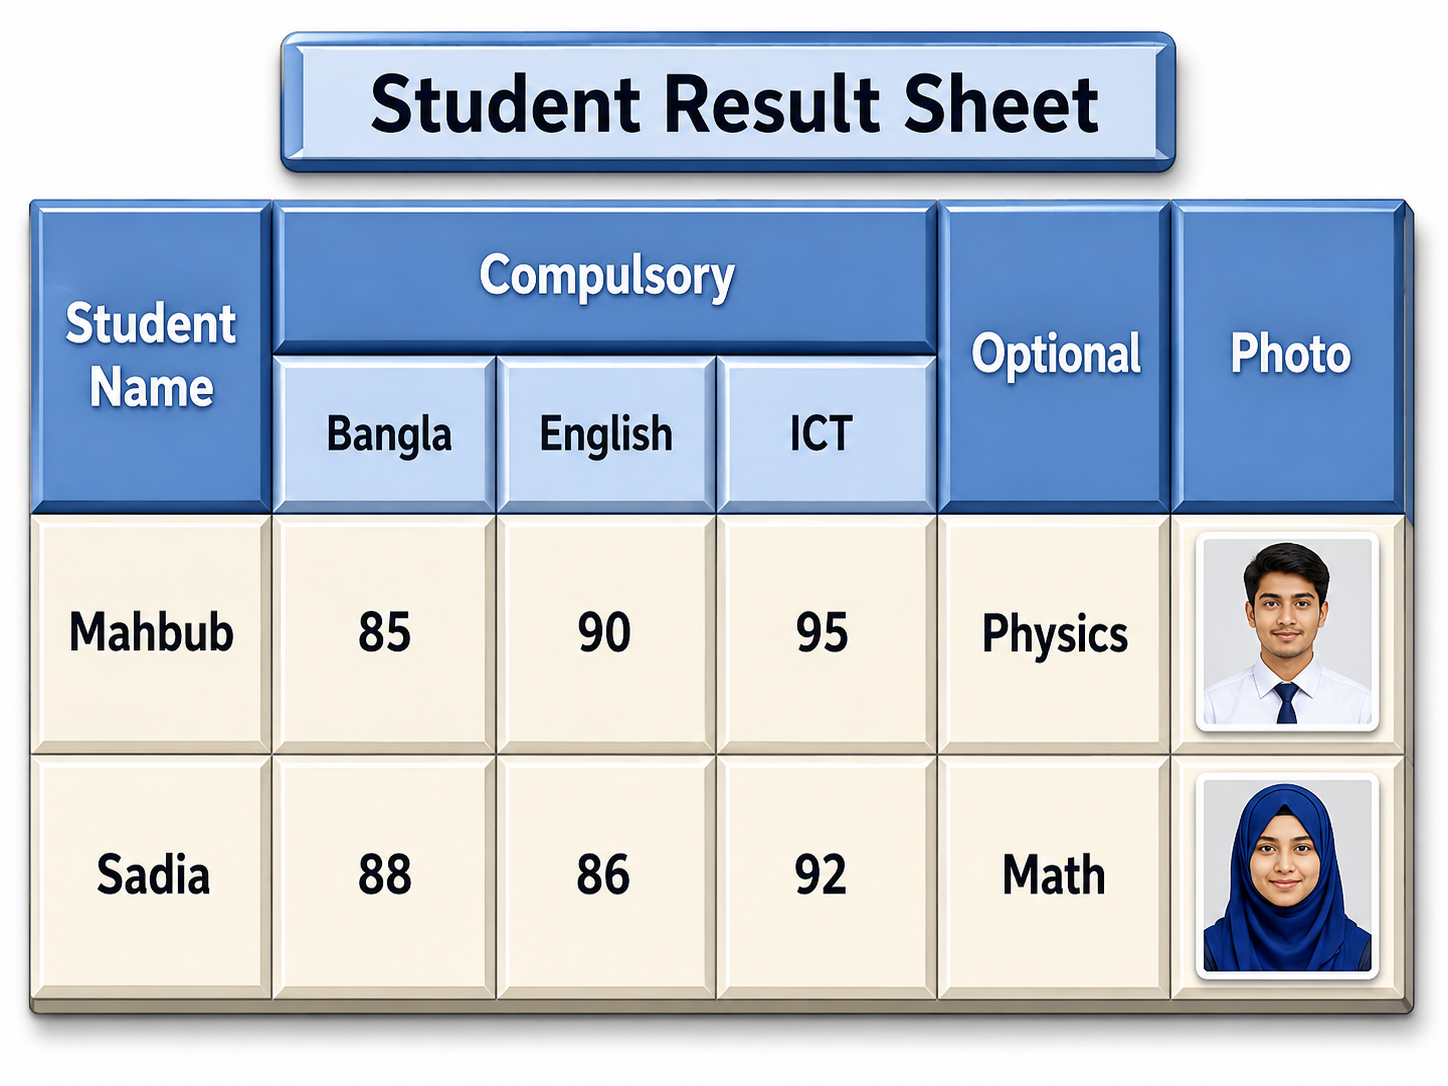
\includegraphics[width=0.95\linewidth,height=0.11\textheight,keepaspectratio]{chapters/Chapter04/topics/images/board_ex56_3d_student_result_mixed.png}
}{
\fbox{\parbox{0.90\linewidth}{\centering\vspace{0.45cm}
\textbf{চিত্র}\\[3pt]
File: \texttt{chapters/Chapter04/topics/images/board\_ex56\_3d\_student\_result\_mixed.png}
\vspace{0.45cm}}}
}
\captionof{figure}{Student Result with Compulsory and Optional Subjects}
\end{center}

\begin{keypointbox}{চিত্র ব্যাখ্যা}
এখানে Student Name, Optional ও Photo header দুই row জুড়ে আছে; Compulsory heading তিনটি column জুড়ে আছে।
\end{keypointbox}

\par\noindent{\color{purple!70!black}\bfseries\small কোড}\par\vspace{-4pt}
\begin{verbatim}
<!DOCTYPE html>
<html>
<head>
  <title>HTML Table Example</title>
</head>
<body>
<table border="1" cellspacing="0" cellpadding="5" align="center">
  <caption><b>Student Result Sheet</b></caption>
  <tr>
    <th rowspan="2">Student Name</th>
    <th colspan="3">Compulsory</th>
    <th rowspan="2">Optional</th>
    <th rowspan="2">Photo</th>
  </tr>
  <tr>
    <th>Bangla</th>
    <th>English</th>
    <th>ICT</th>
  </tr>
  <tr>
    <td>Mahbub</td>
    <td>85</td>
    <td>90</td>
    <td>95</td>
    <td>Physics</td>
    <td><img src="mahbub.jpg" width="60" height="70" alt="Mahbub"></td>
  </tr>
  <tr>
    <td>Sadia</td>
    <td>88</td>
    <td>86</td>
    <td>92</td>
    <td>Math</td>
    <td><img src="sadia.jpg" width="60" height="70" alt="Sadia"></td>
  </tr>
</table>
</body>
</html>
\end{verbatim}
\vspace{-6pt}

\begin{keypointbox}{Board technique}
প্রথমে মোট row ও column গুনবে। তারপর কোন cell horizontal merge হলে \texttt{colspan} এবং vertical merge হলে \texttt{rowspan} ব্যবহার করবে। image-এর জন্য \texttt{<img>} এবং link-এর জন্য \texttt{<a>} tag ব্যবহার করবে।
\end{keypointbox}


\subsubsection{Example 57: Product Catalog with Product Image and Buy Link}

\begin{center}
\IfFileExists{chapters/Chapter04/topics/images/board_ex57_3d_product_catalog_link.png}{
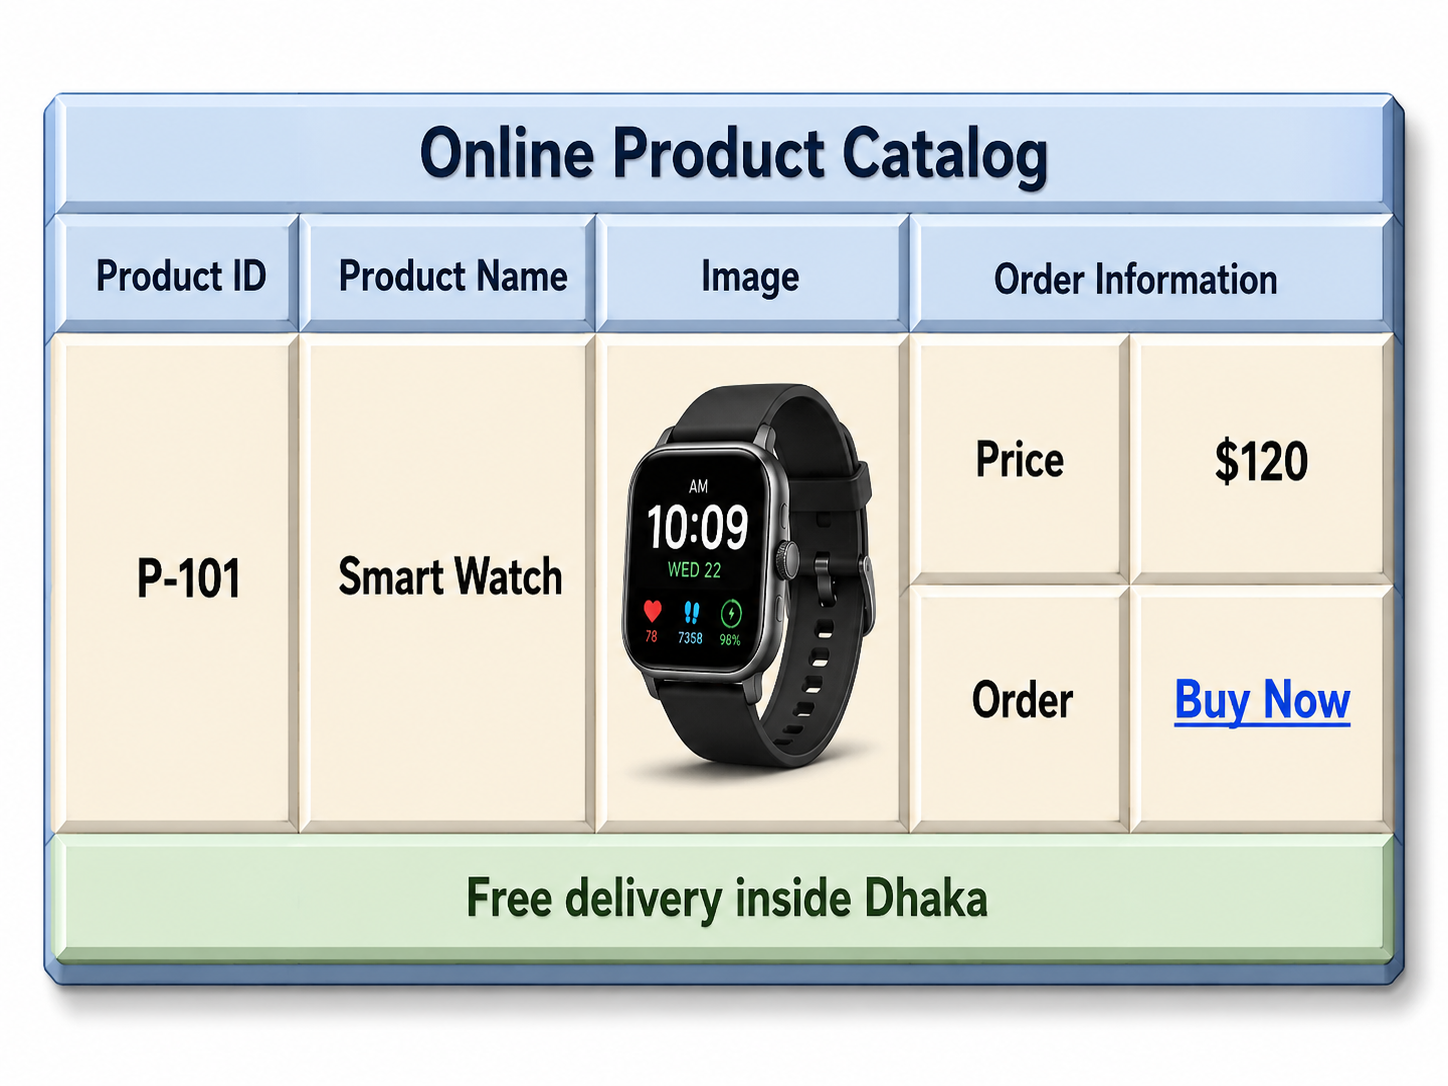
\includegraphics[width=0.95\linewidth,height=0.11\textheight,keepaspectratio]{chapters/Chapter04/topics/images/board_ex57_3d_product_catalog_link.png}
}{
\fbox{\parbox{0.90\linewidth}{\centering\vspace{0.45cm}
\textbf{চিত্র}\\[3pt]
File: \texttt{chapters/Chapter04/topics/images/board\_ex57\_3d\_product\_catalog\_link.png}
\vspace{0.45cm}}}
}
\captionof{figure}{Product Catalog with Product Image and Buy Link}
\end{center}

\begin{keypointbox}{চিত্র ব্যাখ্যা}
Product ID, Name ও Image দুই row জুড়ে রাখা হয়েছে। Order Information দুই column জুড়ে আছে।
\end{keypointbox}

\begin{keypointbox}{চিত্র দেখে code লেখার ধাপ}
প্রথমে figure-এর total row ও column গুনবে। এরপর কোন cell একাধিক column জুড়ে আছে তা দেখে \texttt{colspan} এবং কোন cell একাধিক row জুড়ে আছে তা দেখে \texttt{rowspan} বসাবে। তারপর image, link, list বা nested table থাকলে সংশ্লিষ্ট tag cell-এর ভিতরে লিখবে।
\end{keypointbox}

\par\noindent{\color{purple!70!black}\bfseries\small কোড}\par\vspace{-4pt}
\begin{verbatim}
<!DOCTYPE html>
<html>
<head>
  <title>HTML Table Example</title>
</head>
<body>
<table border="1" cellspacing="0" cellpadding="6" align="center">
  <caption><b>Online Product Catalog</b></caption>
  <tr>
    <th>Product ID</th>
    <th>Product Name</th>
    <th>Image</th>
    <th colspan="2">Order Information</th>
  </tr>
  <tr>
    <td rowspan="2">P-101</td>
    <td rowspan="2">Smart Watch</td>
    <td rowspan="2"><img src="watch.jpg" width="90" height="80" alt="Watch"></td>
    <td>Price</td>
    <td>$120</td>
  </tr>
  <tr>
    <td>Order</td>
    <td><a href="order_watch.html">Buy Now</a></td>
  </tr>
  <tr>
    <td colspan="5" align="center">Free delivery inside Dhaka</td>
  </tr>
</table>
</body>
</html>
\end{verbatim}
\vspace{-6pt}

\begin{keypointbox}{Board technique}
প্রথমে মোট row ও column গুনবে। তারপর কোন cell horizontal merge হলে \texttt{colspan} এবং vertical merge হলে \texttt{rowspan} ব্যবহার করবে। image-এর জন্য \texttt{<img>} এবং link-এর জন্য \texttt{<a>} tag ব্যবহার করবে।
\end{keypointbox}


\subsubsection{Example 58: Hospital Information Table with Picture and Emergency Link}

\begin{center}
\IfFileExists{chapters/Chapter04/topics/images/board_ex58_3d_hospital_info_table.png}{
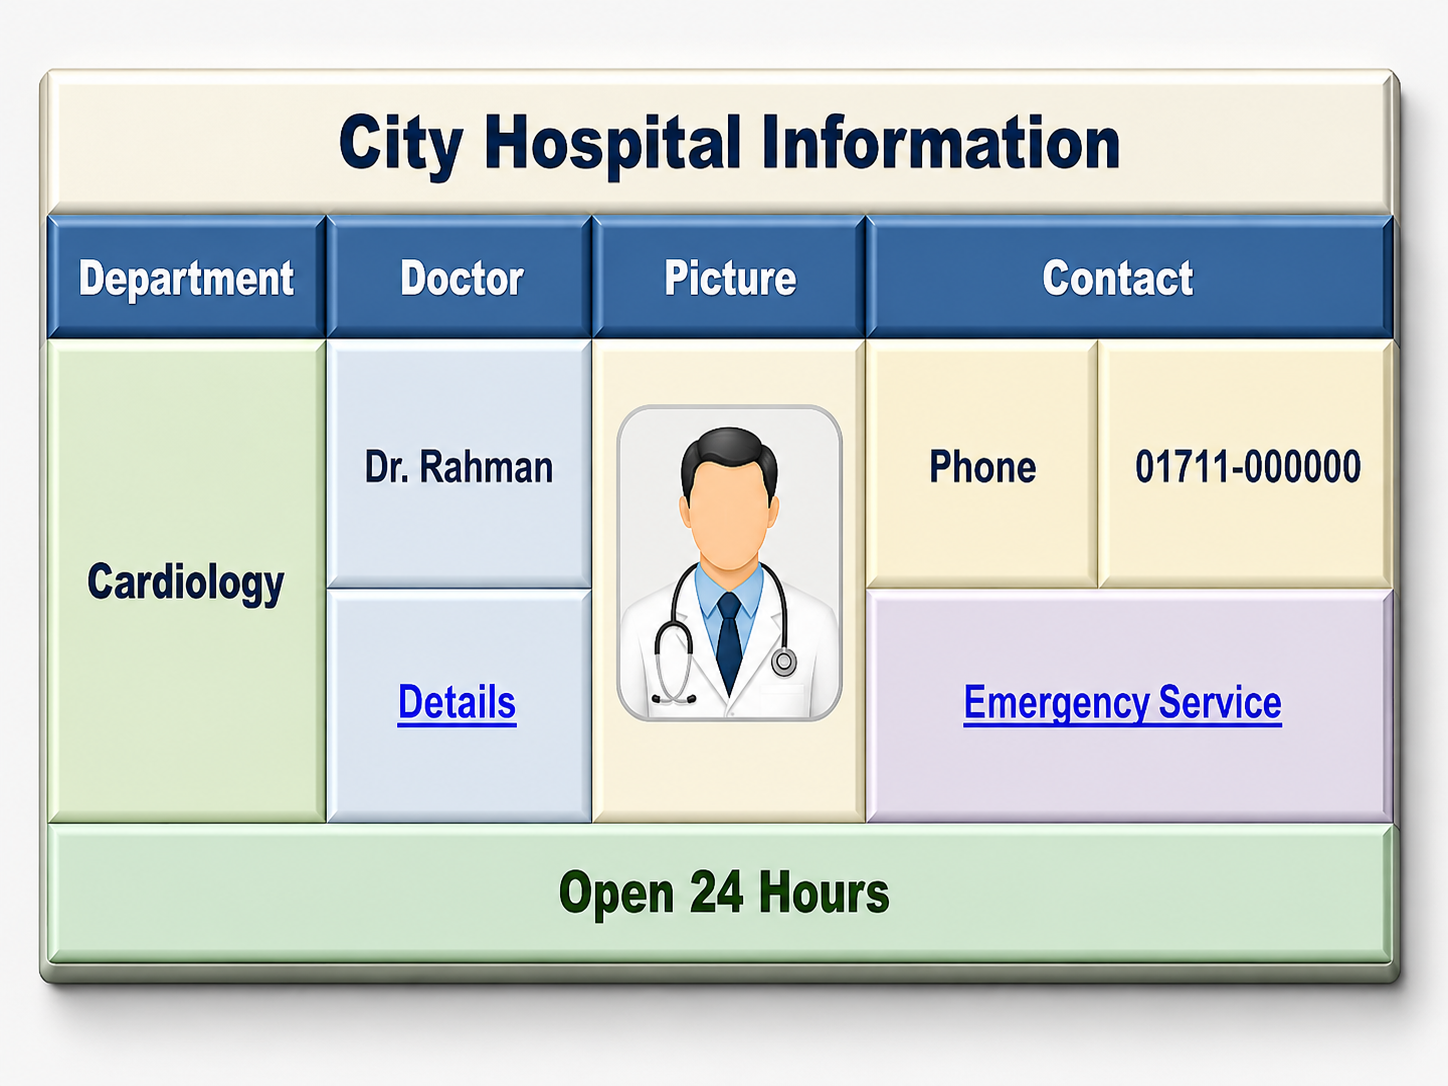
\includegraphics[width=0.95\linewidth,height=0.11\textheight,keepaspectratio]{chapters/Chapter04/topics/images/board_ex58_3d_hospital_info_table.png}
}{
\fbox{\parbox{0.90\linewidth}{\centering\vspace{0.45cm}
\textbf{চিত্র}\\[3pt]
File: \texttt{chapters/Chapter04/topics/images/board\_ex58\_3d\_hospital\_info\_table.png}
\vspace{0.45cm}}}
}
\captionof{figure}{Hospital Information Table with Picture and Emergency Link}
\end{center}

\begin{keypointbox}{চিত্র ব্যাখ্যা}
Cardiology cell এবং doctor image দুই row জুড়ে আছে। Emergency Service link দুইটি contact column জুড়ে দেওয়া হয়েছে।
\end{keypointbox}

\par\noindent{\color{purple!70!black}\bfseries\small কোড}\par\vspace{-4pt}
\begin{verbatim}
<!DOCTYPE html>
<html>
<head>
  <title>HTML Table Example</title>
</head>
<body>
<table border="1" cellspacing="0" cellpadding="6" align="center">
  <caption><b>City Hospital Information</b></caption>
  <tr>
    <th>Department</th>
    <th>Doctor</th>
    <th>Picture</th>
    <th colspan="2">Contact</th>
  </tr>
  <tr>
    <td rowspan="2">Cardiology</td>
    <td>Dr. Rahman</td>
    <td rowspan="2"><img src="doctor.jpg" width="80" height="90" alt="Doctor"></td>
    <td>Phone</td>
    <td>01711-000000</td>
  </tr>
  <tr>
    <td><a href="cardiology.html">Details</a></td>
    <td colspan="2"><a href="emergency.html">Emergency Service</a></td>
  </tr>
  <tr>
    <td colspan="5" align="center">Open 24 Hours</td>
  </tr>
</table>
</body>
</html>
\end{verbatim}
\vspace{-6pt}

\begin{keypointbox}{Board technique}
প্রথমে মোট row ও column গুনবে। তারপর কোন cell horizontal merge হলে \texttt{colspan} এবং vertical merge হলে \texttt{rowspan} ব্যবহার করবে। image-এর জন্য \texttt{<img>} এবং link-এর জন্য \texttt{<a>} tag ব্যবহার করবে।
\end{keypointbox}


\subsubsection{Example 59: Tourism Table with Place Image and Website Link}

\begin{center}
\IfFileExists{chapters/Chapter04/topics/images/board_ex59_3d_tourism_places_link.png}{
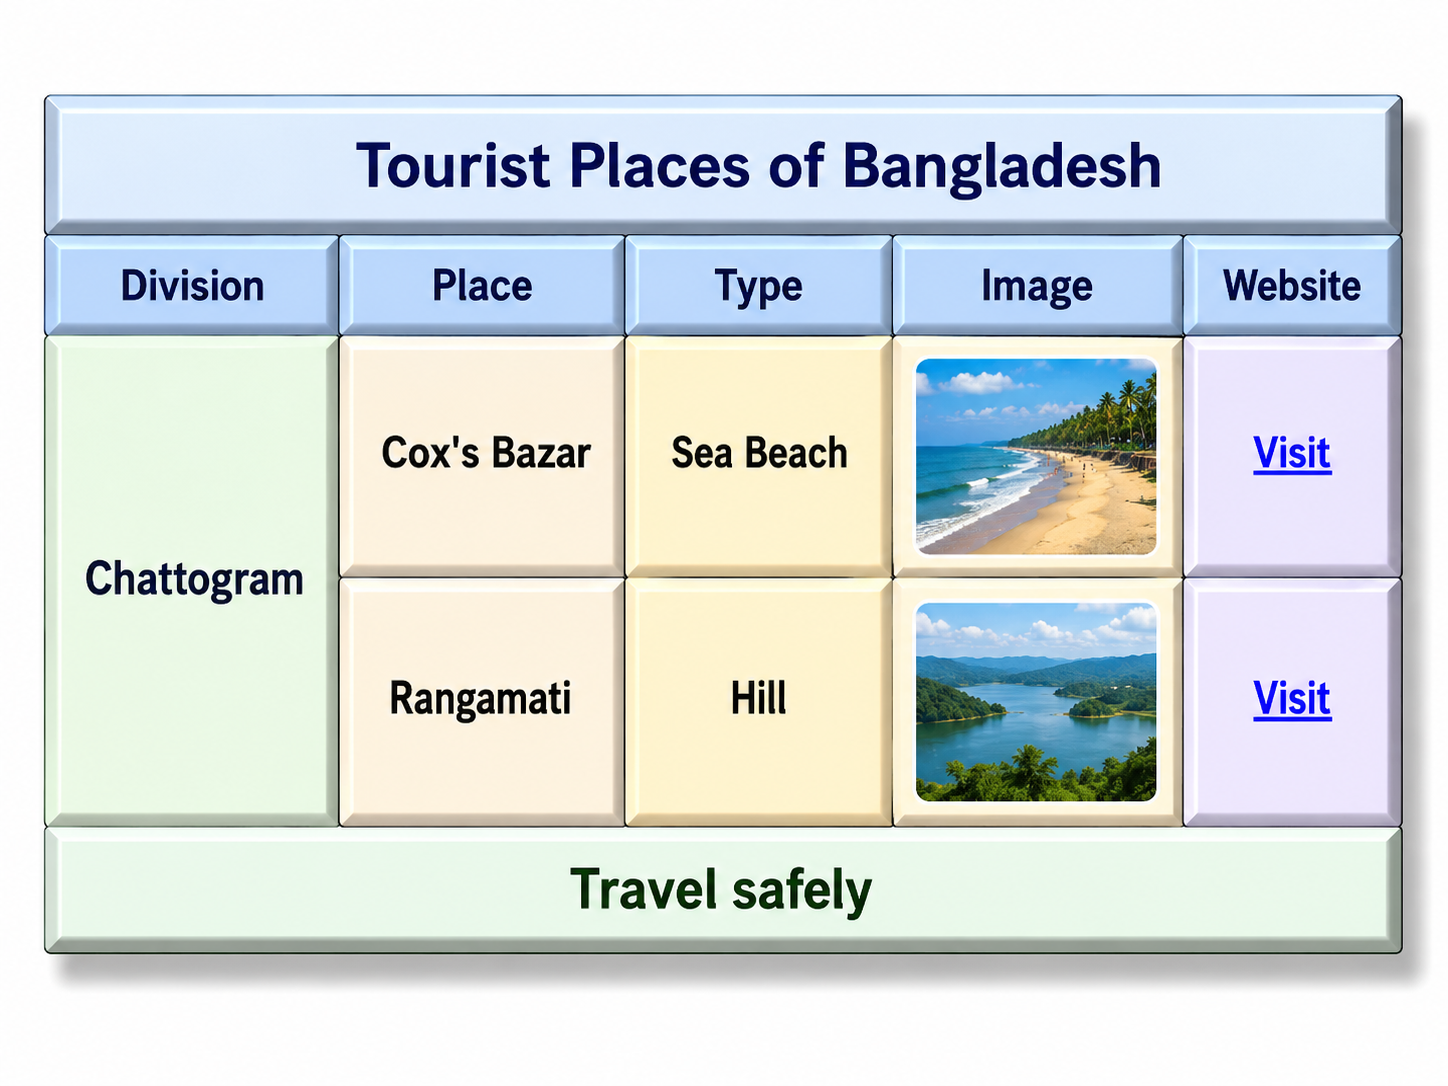
\includegraphics[width=0.95\linewidth,height=0.11\textheight,keepaspectratio]{chapters/Chapter04/topics/images/board_ex59_3d_tourism_places_link.png}
}{
\fbox{\parbox{0.90\linewidth}{\centering\vspace{0.45cm}
\textbf{চিত্র}\\[3pt]
File: \texttt{chapters/Chapter04/topics/images/board\_ex59\_3d\_tourism\_places\_link.png}
\vspace{0.45cm}}}
}
\captionof{figure}{Tourism Table with Place Image and Website Link}
\end{center}

\begin{keypointbox}{চিত্র ব্যাখ্যা}
Division cell rowspan দিয়ে দুই place-এর জন্য common করা হয়েছে। প্রতিটি place-এর image ও link আলাদা cell-এ আছে।
\end{keypointbox}

\begin{keypointbox}{চিত্র দেখে code লেখার ধাপ}
প্রথমে figure-এর total row ও column গুনবে। এরপর কোন cell একাধিক column জুড়ে আছে তা দেখে \texttt{colspan} এবং কোন cell একাধিক row জুড়ে আছে তা দেখে \texttt{rowspan} বসাবে। তারপর image, link, list বা nested table থাকলে সংশ্লিষ্ট tag cell-এর ভিতরে লিখবে।
\end{keypointbox}

\par\noindent{\color{purple!70!black}\bfseries\small কোড}\par\vspace{-4pt}
\begin{verbatim}
<!DOCTYPE html>
<html>
<head>
  <title>HTML Table Example</title>
</head>
<body>
<table border="1" cellspacing="0" cellpadding="5" align="center">
  <caption><b>Tourist Places of Bangladesh</b></caption>
  <tr>
    <th>Division</th>
    <th>Place</th>
    <th>Type</th>
    <th>Image</th>
    <th>Website</th>
  </tr>
  <tr>
    <td rowspan="2">Chattogram</td>
    <td>Cox's Bazar</td>
    <td>Sea Beach</td>
    <td><img src="cox.jpg" width="80" height="60" alt="Cox's Bazar"></td>
    <td><a href="cox.html">Visit</a></td>
  </tr>
  <tr>
    <td>Rangamati</td>
    <td>Hill</td>
    <td><img src="rangamati.jpg" width="80" height="60" alt="Rangamati"></td>
    <td><a href="rangamati.html">Visit</a></td>
  </tr>
  <tr>
    <td colspan="5" align="center">Travel safely</td>
  </tr>
</table>
</body>
</html>
\end{verbatim}
\vspace{-6pt}

\begin{keypointbox}{Board technique}
প্রথমে মোট row ও column গুনবে। তারপর কোন cell horizontal merge হলে \texttt{colspan} এবং vertical merge হলে \texttt{rowspan} ব্যবহার করবে। image-এর জন্য \texttt{<img>} এবং link-এর জন্য \texttt{<a>} tag ব্যবহার করবে।
\end{keypointbox}


\subsubsection{Example 60: Course Plan Table with List, Link and Colspan}

\begin{center}
\IfFileExists{chapters/Chapter04/topics/images/board_ex60_3d_course_plan_list_link.png}{
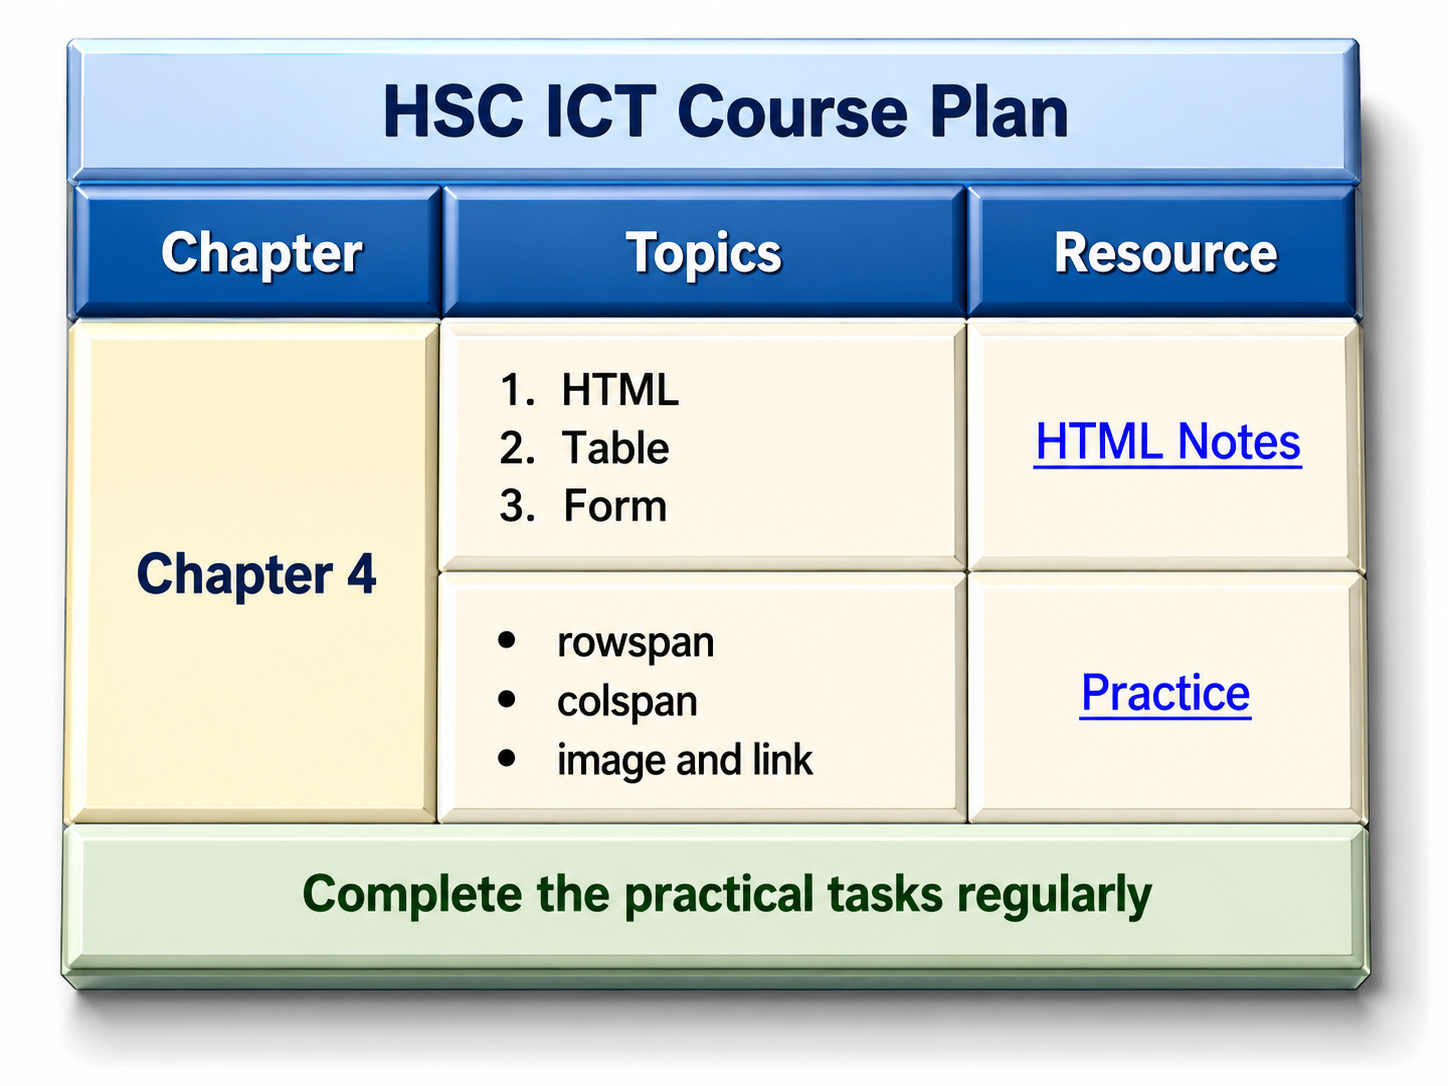
\includegraphics[width=0.95\linewidth,height=0.11\textheight,keepaspectratio]{chapters/Chapter04/topics/images/board_ex60_3d_course_plan_list_link.png}
}{
\fbox{\parbox{0.90\linewidth}{\centering\vspace{0.45cm}
\textbf{চিত্র}\\[3pt]
File: \texttt{chapters/Chapter04/topics/images/board\_ex60\_3d\_course\_plan\_list\_link.png}
\vspace{0.45cm}}}
}
\captionof{figure}{Course Plan Table with List, Link and Colspan}
\end{center}

\begin{keypointbox}{চিত্র ব্যাখ্যা}
একই table cell-এর ভিতরে ordered list ও unordered list রাখা হয়েছে, সাথে hyperlink ও colspan notice আছে।
\end{keypointbox}

\par\noindent{\color{purple!70!black}\bfseries\small কোড}\par\vspace{-4pt}
\begin{verbatim}
<!DOCTYPE html>
<html>
<head>
  <title>HTML Table Example</title>
</head>
<body>
<table border="1" cellspacing="0" cellpadding="6" align="center">
  <caption><b>HSC ICT Course Plan</b></caption>
  <tr>
    <th>Chapter</th>
    <th>Topics</th>
    <th>Resource</th>
  </tr>
  <tr>
    <td rowspan="2">Chapter 4</td>
    <td>
      <ol>
        <li>HTML</li>
        <li>Table</li>
        <li>Form</li>
      </ol>
    </td>
    <td><a href="html_notes.html">HTML Notes</a></td>
  </tr>
  <tr>
    <td>
      <ul>
        <li>rowspan</li>
        <li>colspan</li>
        <li>image and link</li>
      </ul>
    </td>
    <td><a href="practice.html">Practice</a></td>
  </tr>
  <tr>
    <td colspan="3" align="center">Complete the practical tasks regularly</td>
  </tr>
</table>
</body>
</html>
\end{verbatim}
\vspace{-6pt}

\begin{keypointbox}{Board technique}
প্রথমে মোট row ও column গুনবে। তারপর কোন cell horizontal merge হলে \texttt{colspan} এবং vertical merge হলে \texttt{rowspan} ব্যবহার করবে। image-এর জন্য \texttt{<img>} এবং link-এর জন্য \texttt{<a>} tag ব্যবহার করবে।
\end{keypointbox}


\subsubsection{Example 61: Library Book Table with Cover Image and Download Link}

\begin{center}
\IfFileExists{chapters/Chapter04/topics/images/board_ex61_3d_library_book_table.png}{
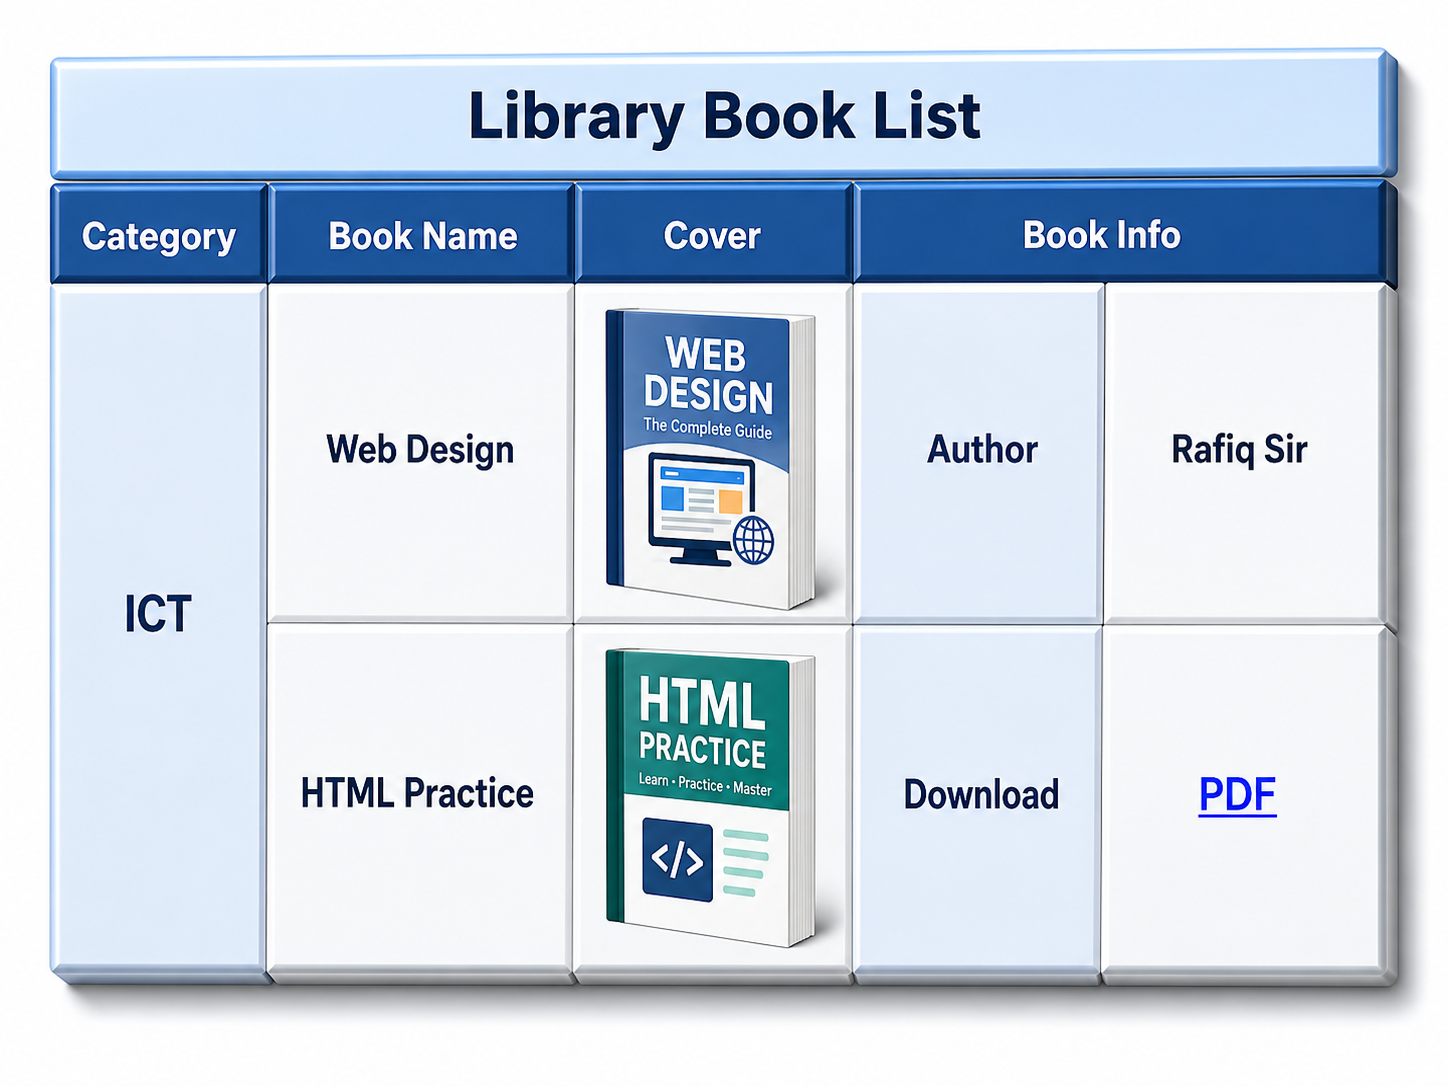
\includegraphics[width=0.95\linewidth,height=0.11\textheight,keepaspectratio]{chapters/Chapter04/topics/images/board_ex61_3d_library_book_table.png}
}{
\fbox{\parbox{0.90\linewidth}{\centering\vspace{0.45cm}
\textbf{চিত্র}\\[3pt]
File: \texttt{chapters/Chapter04/topics/images/board\_ex61\_3d\_library\_book\_table.png}
\vspace{0.45cm}}}
}
\captionof{figure}{Library Book Table with Cover Image and Download Link}
\end{center}

\begin{keypointbox}{চিত্র ব্যাখ্যা}
Category rowspan দিয়ে দুই বইকে একই category-তে দেখানো হয়েছে। Cover image ও PDF link দুই ধরনের content দেখানো হয়েছে।
\end{keypointbox}

\begin{keypointbox}{চিত্র দেখে code লেখার ধাপ}
প্রথমে figure-এর total row ও column গুনবে। এরপর কোন cell একাধিক column জুড়ে আছে তা দেখে \texttt{colspan} এবং কোন cell একাধিক row জুড়ে আছে তা দেখে \texttt{rowspan} বসাবে। তারপর image, link, list বা nested table থাকলে সংশ্লিষ্ট tag cell-এর ভিতরে লিখবে।
\end{keypointbox}

\par\noindent{\color{purple!70!black}\bfseries\small কোড}\par\vspace{-4pt}
\begin{verbatim}
<!DOCTYPE html>
<html>
<head>
  <title>HTML Table Example</title>
</head>
<body>
<table border="1" cellspacing="0" cellpadding="6" align="center">
  <caption><b>Library Book List</b></caption>
  <tr>
    <th>Category</th>
    <th>Book Name</th>
    <th>Cover</th>
    <th colspan="2">Book Info</th>
  </tr>
  <tr>
    <td rowspan="2">ICT</td>
    <td>Web Design</td>
    <td><img src="web_book.jpg" width="70" height="90" alt="Web Book"></td>
    <td>Author</td>
    <td>Rafiq Sir</td>
  </tr>
  <tr>
    <td>HTML Practice</td>
    <td><img src="html_book.jpg" width="70" height="90" alt="HTML Book"></td>
    <td>Download</td>
    <td><a href="html_practice.pdf">PDF</a></td>
  </tr>
</table>
</body>
</html>
\end{verbatim}
\vspace{-6pt}

\begin{keypointbox}{Board technique}
প্রথমে মোট row ও column গুনবে। তারপর কোন cell horizontal merge হলে \texttt{colspan} এবং vertical merge হলে \texttt{rowspan} ব্যবহার করবে। image-এর জন্য \texttt{<img>} এবং link-এর জন্য \texttt{<a>} tag ব্যবহার করবে।
\end{keypointbox}


\subsubsection{Example 62: Exam Routine with Date Rowspan and Subject Colspan}

\begin{center}
\IfFileExists{chapters/Chapter04/topics/images/board_ex62_3d_exam_routine_table.png}{
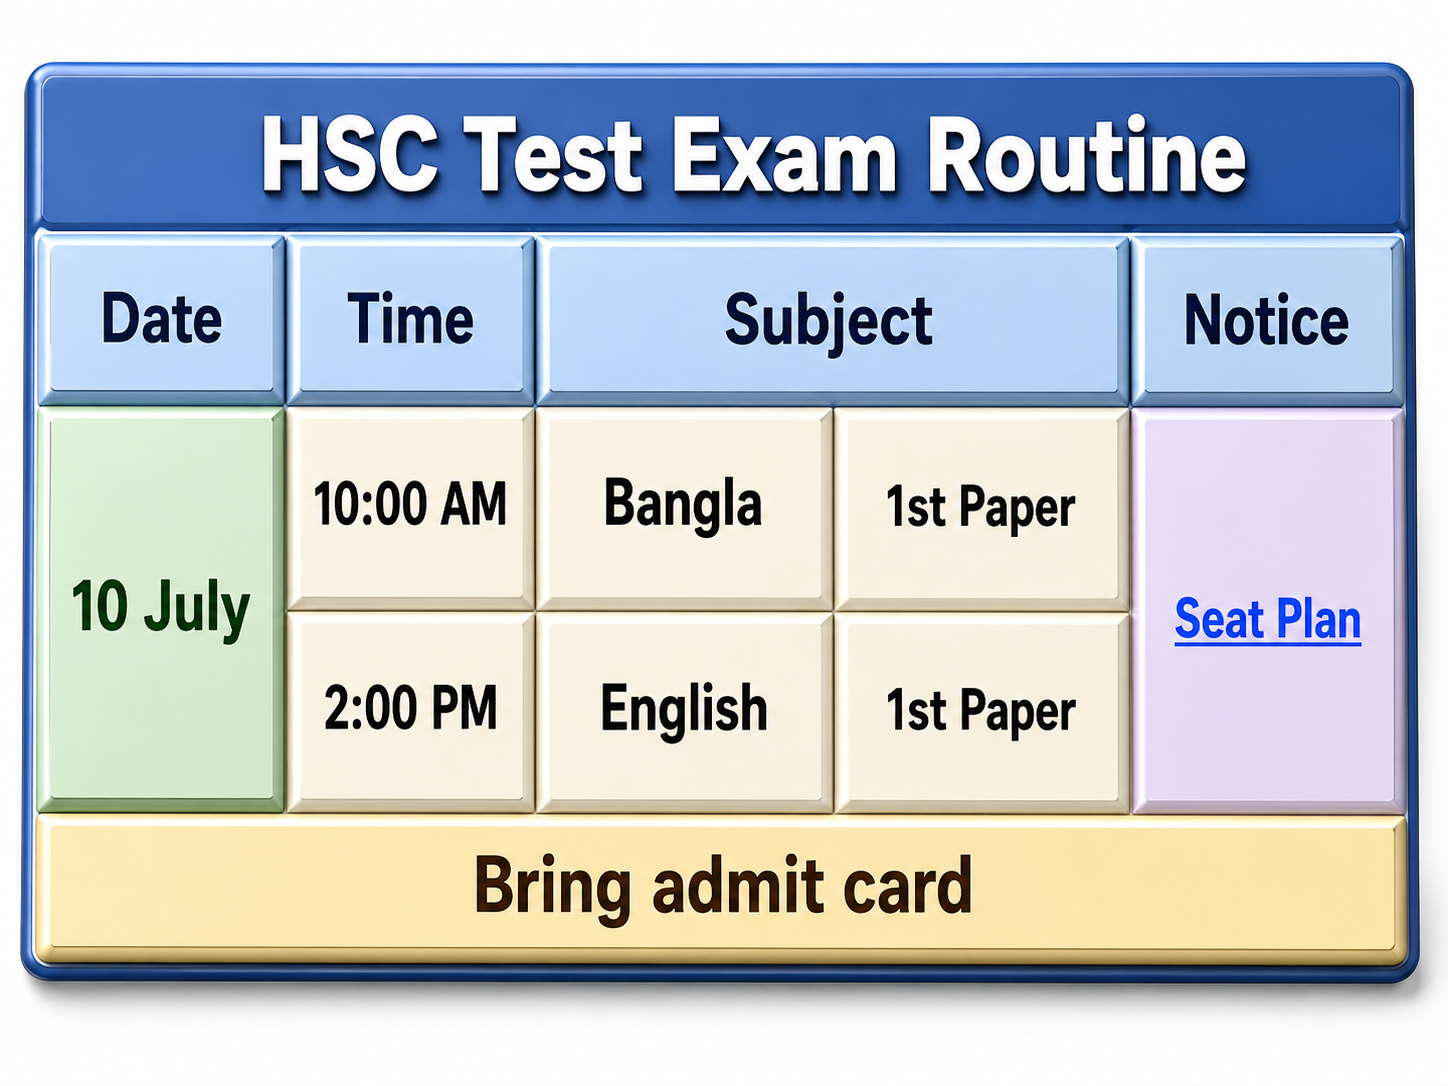
\includegraphics[width=0.95\linewidth,height=0.11\textheight,keepaspectratio]{chapters/Chapter04/topics/images/board_ex62_3d_exam_routine_table.png}
}{
\fbox{\parbox{0.90\linewidth}{\centering\vspace{0.45cm}
\textbf{চিত্র}\\[3pt]
File: \texttt{chapters/Chapter04/topics/images/board\_ex62\_3d\_exam\_routine\_table.png}
\vspace{0.45cm}}}
}
\captionof{figure}{Exam Routine with Date Rowspan and Subject Colspan}
\end{center}

\begin{keypointbox}{চিত্র ব্যাখ্যা}
একই তারিখের দুই exam দেখাতে Date এবং Notice cell-এ rowspan ব্যবহার করা হয়েছে। Subject heading দুই column জুড়ে আছে।
\end{keypointbox}

\par\noindent{\color{purple!70!black}\bfseries\small কোড}\par\vspace{-4pt}
\begin{verbatim}
<!DOCTYPE html>
<html>
<head>
  <title>HTML Table Example</title>
</head>
<body>
<table border="1" cellspacing="0" cellpadding="6" align="center">
  <caption><b>HSC Test Exam Routine</b></caption>
  <tr>
    <th>Date</th>
    <th>Time</th>
    <th colspan="2">Subject</th>
    <th>Notice</th>
  </tr>
  <tr>
    <td rowspan="2">10 July</td>
    <td>10:00 AM</td>
    <td>Bangla</td>
    <td>1st Paper</td>
    <td rowspan="2"><a href="seat_plan.html">Seat Plan</a></td>
  </tr>
  <tr>
    <td>2:00 PM</td>
    <td>English</td>
    <td>1st Paper</td>
  </tr>
  <tr>
    <td colspan="5" align="center">Bring admit card</td>
  </tr>
</table>
</body>
</html>
\end{verbatim}
\vspace{-6pt}

\begin{keypointbox}{Board technique}
প্রথমে মোট row ও column গুনবে। তারপর কোন cell horizontal merge হলে \texttt{colspan} এবং vertical merge হলে \texttt{rowspan} ব্যবহার করবে। image-এর জন্য \texttt{<img>} এবং link-এর জন্য \texttt{<a>} tag ব্যবহার করবে।
\end{keypointbox}


\subsubsection{Example 63: ICT Lab Inventory with Device Image and Manual Link}

\begin{center}
\IfFileExists{chapters/Chapter04/topics/images/board_ex63_3d_lab_inventory_table.png}{
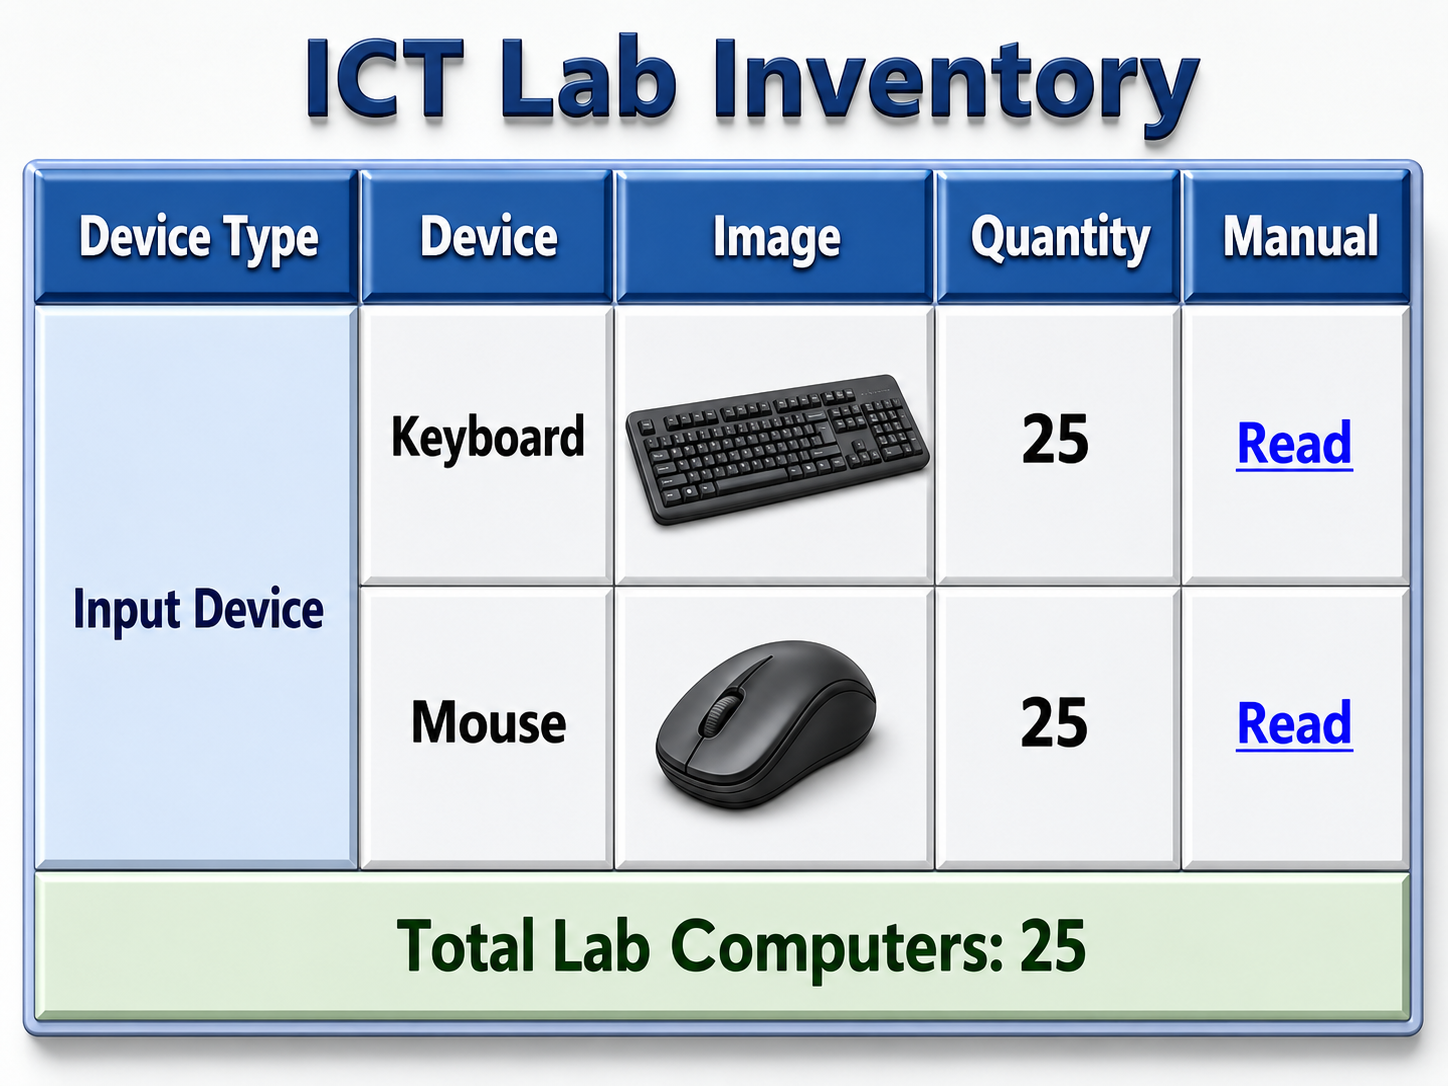
\includegraphics[width=0.95\linewidth,height=0.11\textheight,keepaspectratio]{chapters/Chapter04/topics/images/board_ex63_3d_lab_inventory_table.png}
}{
\fbox{\parbox{0.90\linewidth}{\centering\vspace{0.45cm}
\textbf{চিত্র}\\[3pt]
File: \texttt{chapters/Chapter04/topics/images/board\_ex63\_3d\_lab\_inventory\_table.png}
\vspace{0.45cm}}}
}
\captionof{figure}{ICT Lab Inventory with Device Image and Manual Link}
\end{center}

\begin{keypointbox}{চিত্র ব্যাখ্যা}
Device Type rowspan দিয়ে দুই input device group করা হয়েছে। প্রতিটি device-এর image ও manual link আছে।
\end{keypointbox}

\begin{keypointbox}{চিত্র দেখে code লেখার ধাপ}
প্রথমে figure-এর total row ও column গুনবে। এরপর কোন cell একাধিক column জুড়ে আছে তা দেখে \texttt{colspan} এবং কোন cell একাধিক row জুড়ে আছে তা দেখে \texttt{rowspan} বসাবে। তারপর image, link, list বা nested table থাকলে সংশ্লিষ্ট tag cell-এর ভিতরে লিখবে।
\end{keypointbox}

\par\noindent{\color{purple!70!black}\bfseries\small কোড}\par\vspace{-4pt}
\begin{verbatim}
<!DOCTYPE html>
<html>
<head>
  <title>HTML Table Example</title>
</head>
<body>
<table border="1" cellspacing="0" cellpadding="6" align="center">
  <caption><b>ICT Lab Inventory</b></caption>
  <tr>
    <th>Device Type</th>
    <th>Device</th>
    <th>Image</th>
    <th>Quantity</th>
    <th>Manual</th>
  </tr>
  <tr>
    <td rowspan="2">Input Device</td>
    <td>Keyboard</td>
    <td><img src="keyboard.jpg" width="80" height="50" alt="Keyboard"></td>
    <td>25</td>
    <td><a href="keyboard.html">Read</a></td>
  </tr>
  <tr>
    <td>Mouse</td>
    <td><img src="mouse.jpg" width="80" height="50" alt="Mouse"></td>
    <td>25</td>
    <td><a href="mouse.html">Read</a></td>
  </tr>
  <tr>
    <td colspan="5" align="center">Total Lab Computers: 25</td>
  </tr>
</table>
</body>
</html>
\end{verbatim}
\vspace{-6pt}

\begin{keypointbox}{Board technique}
প্রথমে মোট row ও column গুনবে। তারপর কোন cell horizontal merge হলে \texttt{colspan} এবং vertical merge হলে \texttt{rowspan} ব্যবহার করবে। image-এর জন্য \texttt{<img>} এবং link-এর জন্য \texttt{<a>} tag ব্যবহার করবে।
\end{keypointbox}


\subsubsection{Example 64: Restaurant Menu with Specials, Image, Link and Colspan}

\begin{center}
\IfFileExists{chapters/Chapter04/topics/images/board_ex64_3d_restaurant_menu_mixed.png}{
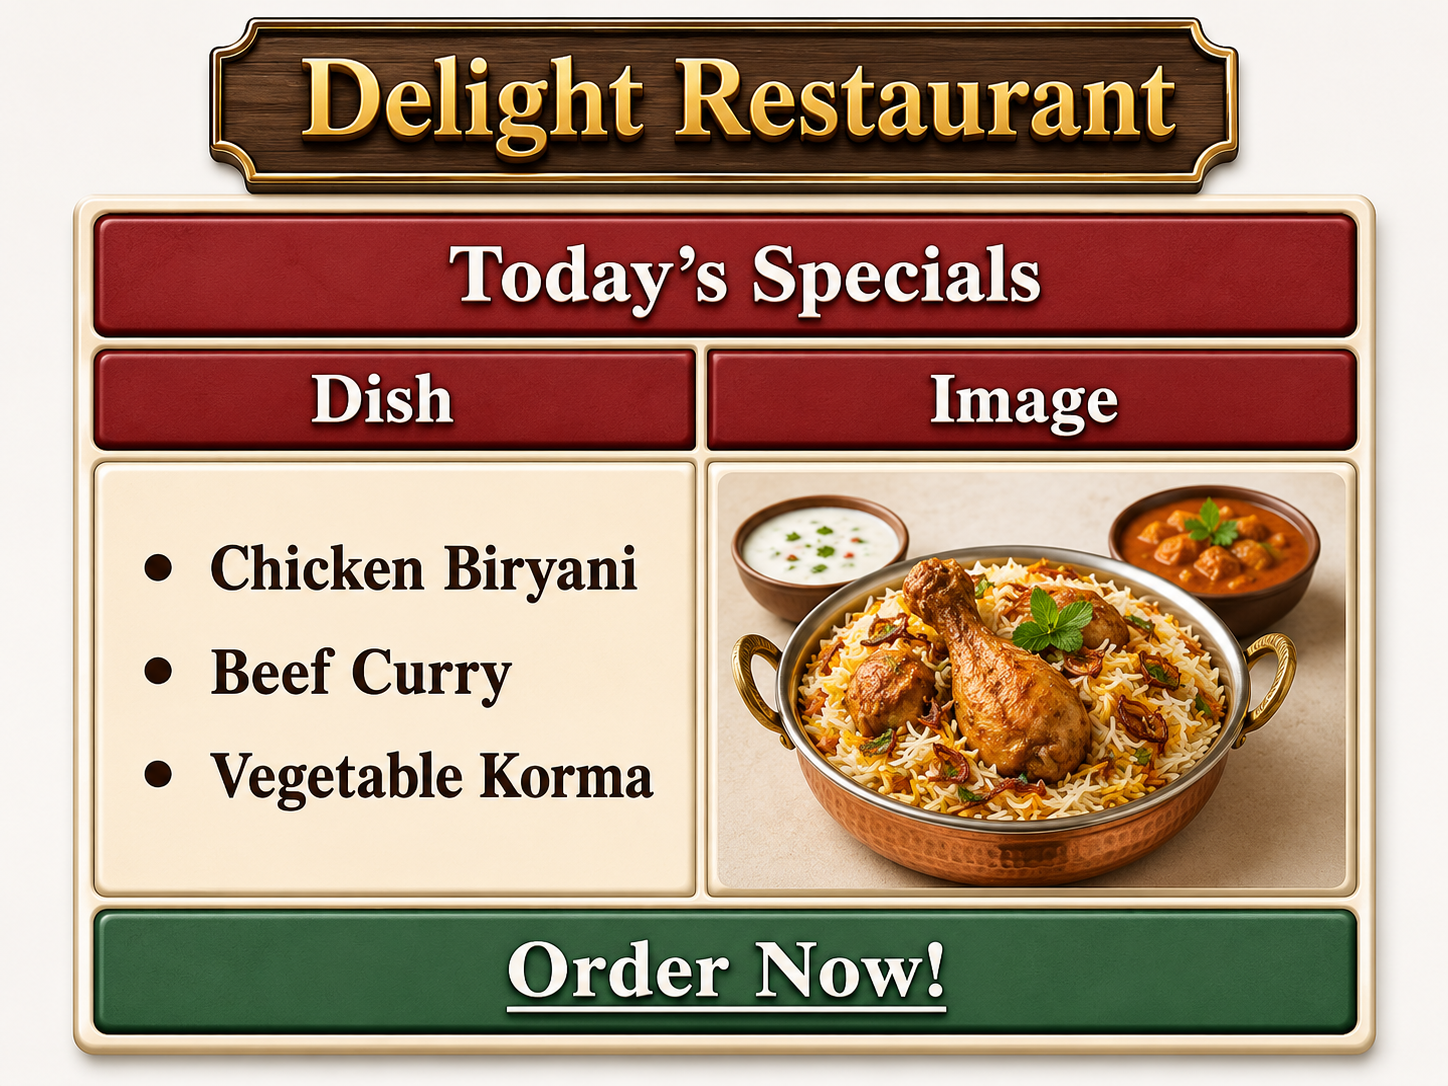
\includegraphics[width=0.95\linewidth,height=0.11\textheight,keepaspectratio]{chapters/Chapter04/topics/images/board_ex64_3d_restaurant_menu_mixed.png}
}{
\fbox{\parbox{0.90\linewidth}{\centering\vspace{0.45cm}
\textbf{চিত্র}\\[3pt]
File: \texttt{chapters/Chapter04/topics/images/board\_ex64\_3d\_restaurant\_menu\_mixed.png}
\vspace{0.45cm}}}
}
\captionof{figure}{Restaurant menu with specials, image and colspan}
\end{center}

\begin{keypointbox}{চিত্র ব্যাখ্যা}
চিত্রে Delight Restaurant heading, Today's Specials title row, Dish ও Image দুইটি column, item list, food image এবং নিচে full-width Order Now row আছে।
\end{keypointbox}

\begin{keypointbox}{চিত্র দেখে code লেখার ধাপ}
প্রথমে restaurant heading লিখবে। তারপর two-column table বানাবে। Today's Specials row এবং Order Now row দুই column জুড়ে থাকবে, তাই দুই জায়গায় \texttt{colspan="2"} ব্যবহার করবে। Dish cell-এ list/line break এবং Image cell-এ \texttt{<img>} tag বসাবে।
\end{keypointbox}

\par\noindent{\color{purple!70!black}\bfseries\small কোড}\par\vspace{-4pt}
\begin{verbatim}
<!DOCTYPE html>
<html>
<head>
  <title>HTML Table Example</title>
</head>
<body>
<h2 align="center">Delight Restaurant</h2>
<table border="1" cellspacing="0" cellpadding="8" align="center">
  <tr>
    <th colspan="2">Today's Specials</th>
  </tr>
  <tr>
    <th>Dish</th>
    <th>Image</th>
  </tr>
  <tr>
    <td>
      <ul>
        <li>Chicken Biryani</li>
        <li>Beef Curry</li>
        <li>Vegetable Korma</li>
      </ul>
    </td>
    <td><img src="food.jpg" width="100" height="80" alt="Food"></td>
  </tr>
  <tr>
    <td colspan="2" align="center"><a href="order.html">Order Now!</a></td>
  </tr>
</table>
</body>
</html>
\end{verbatim}
\vspace{-6pt}

\begin{keypointbox}{Board technique}
প্রথমে মোট row ও column গুনবে। তারপর কোন cell horizontal merge হলে \texttt{colspan} এবং vertical merge হলে \texttt{rowspan} ব্যবহার করবে। image-এর জন্য \texttt{<img>} এবং link-এর জন্য \texttt{<a>} tag ব্যবহার করবে।
\end{keypointbox}

\subsubsection{Example 65: Student Club Table with Rowspan and Image Icon}

\begin{center}
\IfFileExists{chapters/Chapter04/topics/images/board_ex65_3d_student_club_table.png}{
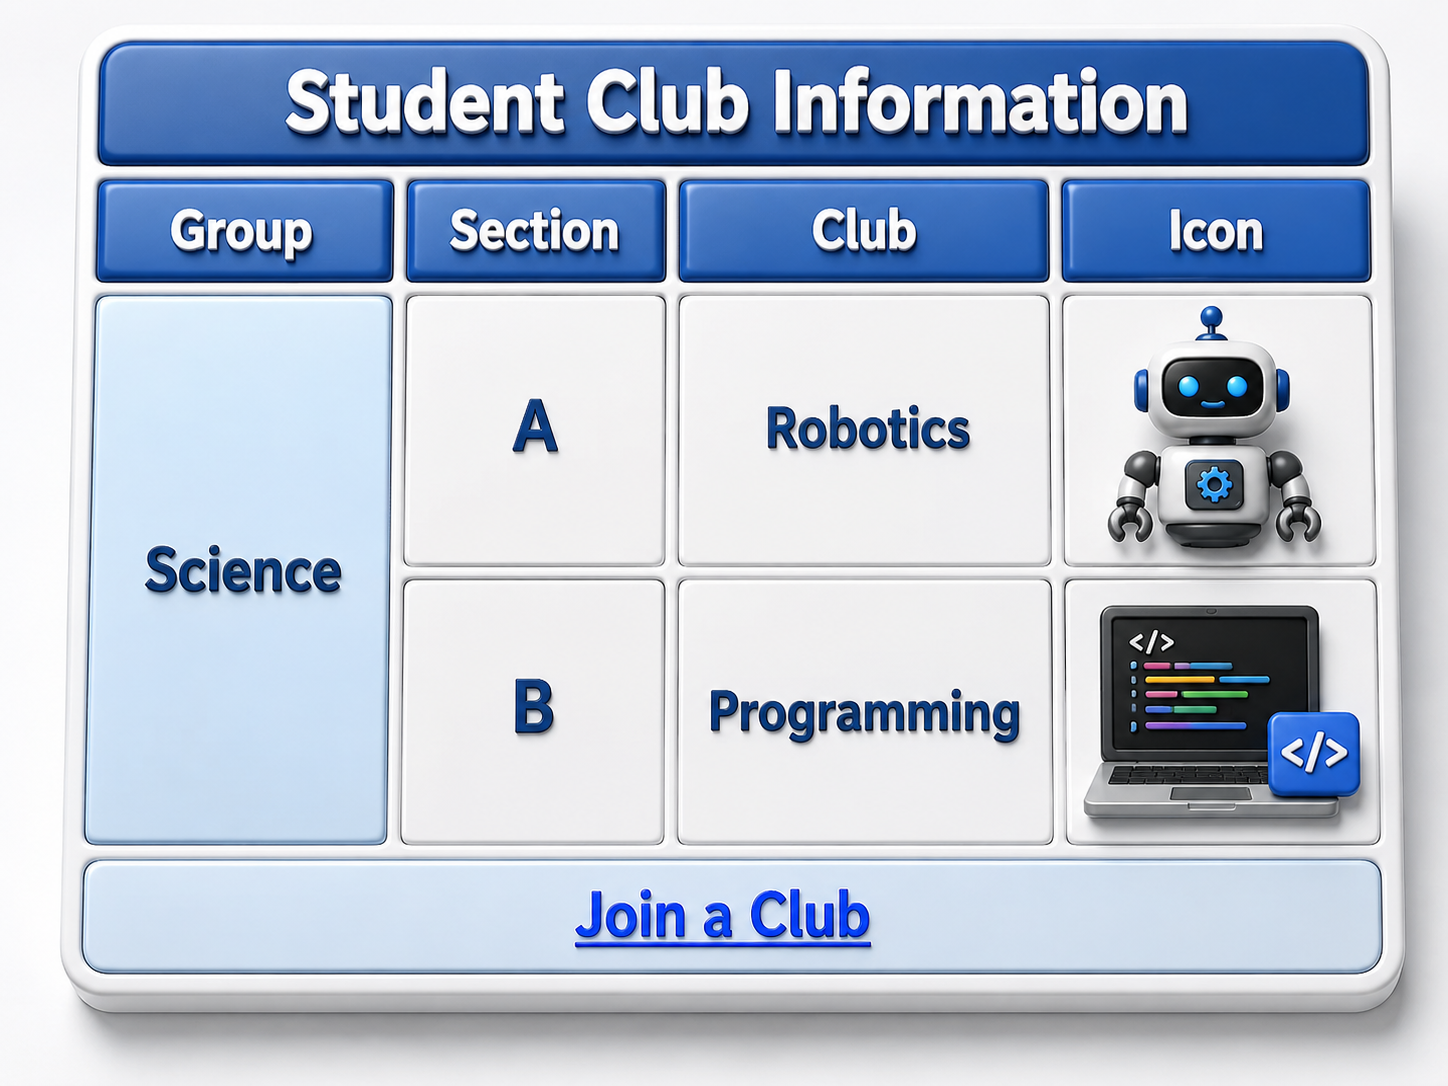
\includegraphics[width=0.95\linewidth,height=0.11\textheight,keepaspectratio]{chapters/Chapter04/topics/images/board_ex65_3d_student_club_table.png}
}{
\fbox{\parbox{0.90\linewidth}{\centering\vspace{0.45cm}
\textbf{চিত্র}\\[3pt]
File: \texttt{chapters/Chapter04/topics/images/board\_ex65\_3d\_student\_club\_table.png}
\vspace{0.45cm}}}
}
\captionof{figure}{Student Club Table with Rowspan and Image Icon}
\end{center}

\begin{keypointbox}{চিত্র ব্যাখ্যা}
Science group-এর দুই section দেখাতে rowspan, club icon দেখাতে image এবং join link দেখাতে colspan ব্যবহার করা হয়েছে।
\end{keypointbox}

\begin{keypointbox}{চিত্র দেখে code লেখার ধাপ}
প্রথমে figure-এর total row ও column গুনবে। এরপর কোন cell একাধিক column জুড়ে আছে তা দেখে \texttt{colspan} এবং কোন cell একাধিক row জুড়ে আছে তা দেখে \texttt{rowspan} বসাবে। তারপর image, link, list বা nested table থাকলে সংশ্লিষ্ট tag cell-এর ভিতরে লিখবে।
\end{keypointbox}

\par\noindent{\color{purple!70!black}\bfseries\small কোড}\par\vspace{-4pt}
\begin{verbatim}
<!DOCTYPE html>
<html>
<head>
  <title>HTML Table Example</title>
</head>
<body>
<table border="1" cellspacing="0" cellpadding="6" align="center">
  <caption><b>Student Club Information</b></caption>
  <tr>
    <th>Group</th>
    <th>Section</th>
    <th>Club</th>
    <th>Icon</th>
  </tr>
  <tr>
    <td rowspan="2">Science</td>
    <td>A</td>
    <td>Robotics</td>
    <td><img src="robot.png" width="50" height="50" alt="Robot"></td>
  </tr>
  <tr>
    <td>B</td>
    <td>Programming</td>
    <td><img src="code.png" width="50" height="50" alt="Code"></td>
  </tr>
  <tr>
    <td colspan="4" align="center"><a href="club.html">Join a Club</a></td>
  </tr>
</table>
</body>
</html>
\end{verbatim}
\vspace{-6pt}

\begin{keypointbox}{Board technique}
প্রথমে মোট row ও column গুনবে। তারপর কোন cell horizontal merge হলে \texttt{colspan} এবং vertical merge হলে \texttt{rowspan} ব্যবহার করবে। image-এর জন্য \texttt{<img>} এবং link-এর জন্য \texttt{<a>} tag ব্যবহার করবে।
\end{keypointbox}


\subsubsection{Example 66: Blood Donor Table with Contact Colspan}

\begin{center}
\IfFileExists{chapters/Chapter04/topics/images/board_ex66_3d_blood_donor_contact.png}{
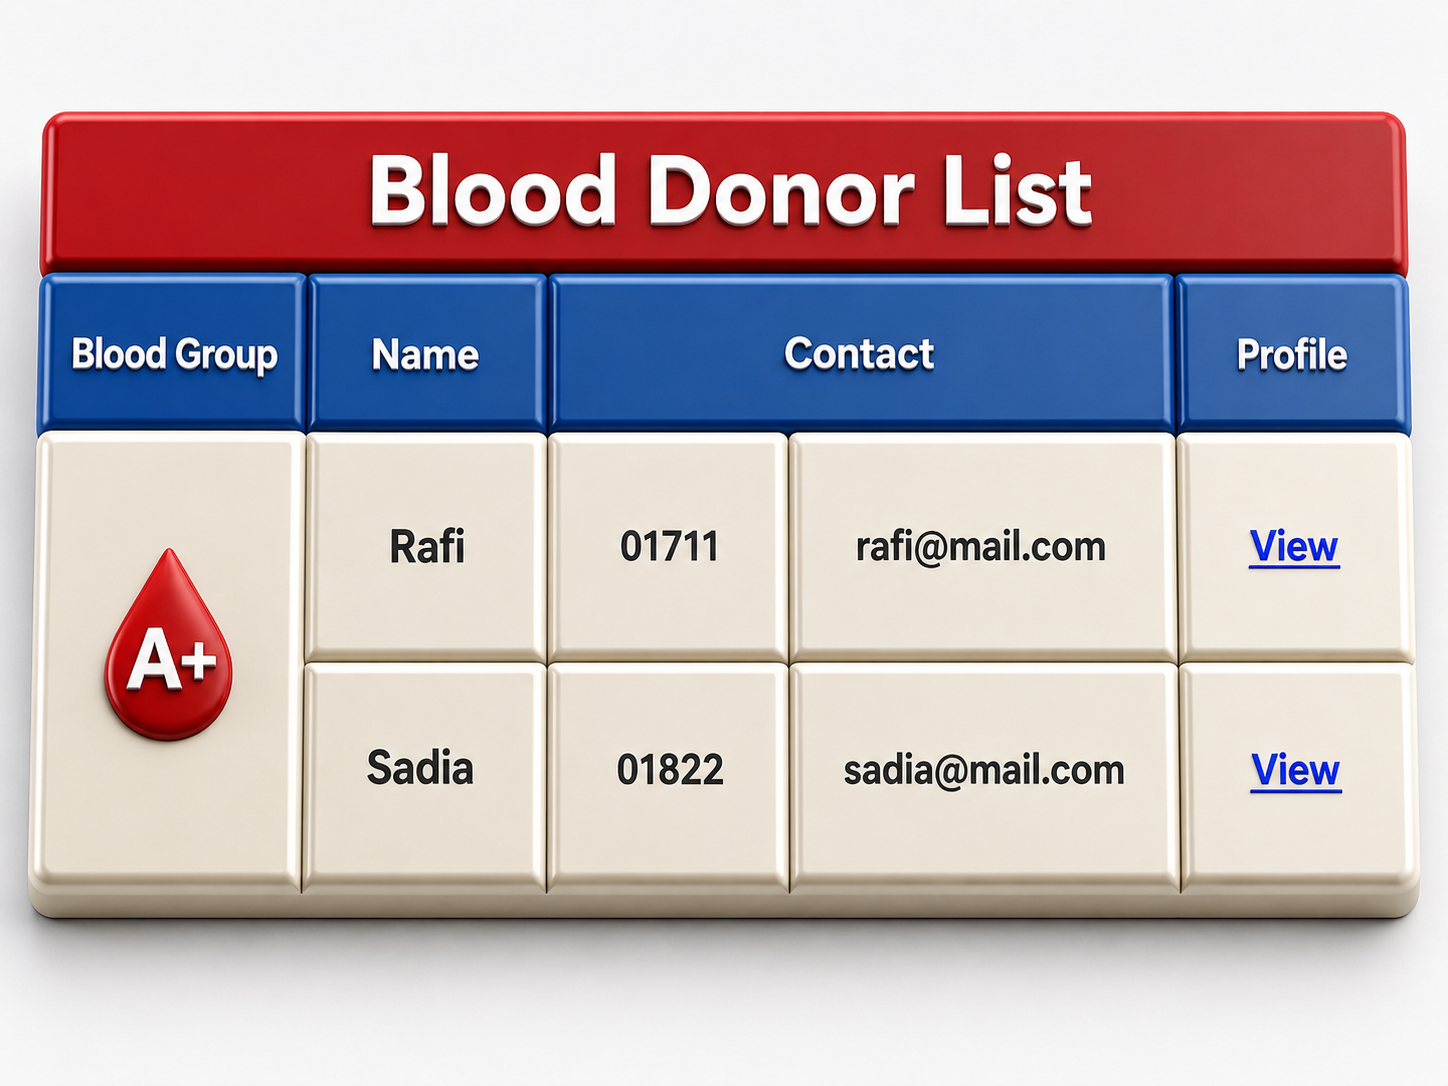
\includegraphics[width=0.95\linewidth,height=0.11\textheight,keepaspectratio]{chapters/Chapter04/topics/images/board_ex66_3d_blood_donor_contact.png}
}{
\fbox{\parbox{0.90\linewidth}{\centering\vspace{0.45cm}
\textbf{চিত্র}\\[3pt]
File: \texttt{chapters/Chapter04/topics/images/board\_ex66\_3d\_blood\_donor\_contact.png}
\vspace{0.45cm}}}
}
\captionof{figure}{Blood Donor Table with Contact Colspan}
\end{center}

\begin{keypointbox}{চিত্র ব্যাখ্যা}
Contact heading দুই column জুড়ে আছে এবং A+ blood group দুই donor-এর জন্য rowspan করা হয়েছে।
\end{keypointbox}

\par\noindent{\color{purple!70!black}\bfseries\small কোড}\par\vspace{-4pt}
\begin{verbatim}
<!DOCTYPE html>
<html>
<head>
  <title>HTML Table Example</title>
</head>
<body>
<table border="1" cellspacing="0" cellpadding="6" align="center">
  <caption><b>Blood Donor List</b></caption>
  <tr>
    <th>Blood Group</th>
    <th>Name</th>
    <th colspan="2">Contact</th>
    <th>Profile</th>
  </tr>
  <tr>
    <td rowspan="2">A+</td>
    <td>Rafi</td>
    <td>01711</td>
    <td>rafi@mail.com</td>
    <td><a href="rafi.html">View</a></td>
  </tr>
  <tr>
    <td>Sadia</td>
    <td>01822</td>
    <td>sadia@mail.com</td>
    <td><a href="sadia.html">View</a></td>
  </tr>
</table>
</body>
</html>
\end{verbatim}
\vspace{-6pt}

\begin{keypointbox}{Board technique}
প্রথমে মোট row ও column গুনবে। তারপর কোন cell horizontal merge হলে \texttt{colspan} এবং vertical merge হলে \texttt{rowspan} ব্যবহার করবে। image-এর জন্য \texttt{<img>} এবং link-এর জন্য \texttt{<a>} tag ব্যবহার করবে।
\end{keypointbox}


\subsubsection{Example 67: Scholarship Table with Logo, Link and Merged Eligibility}

\begin{center}
\IfFileExists{chapters/Chapter04/topics/images/board_ex67_3d_scholarship_table.png}{
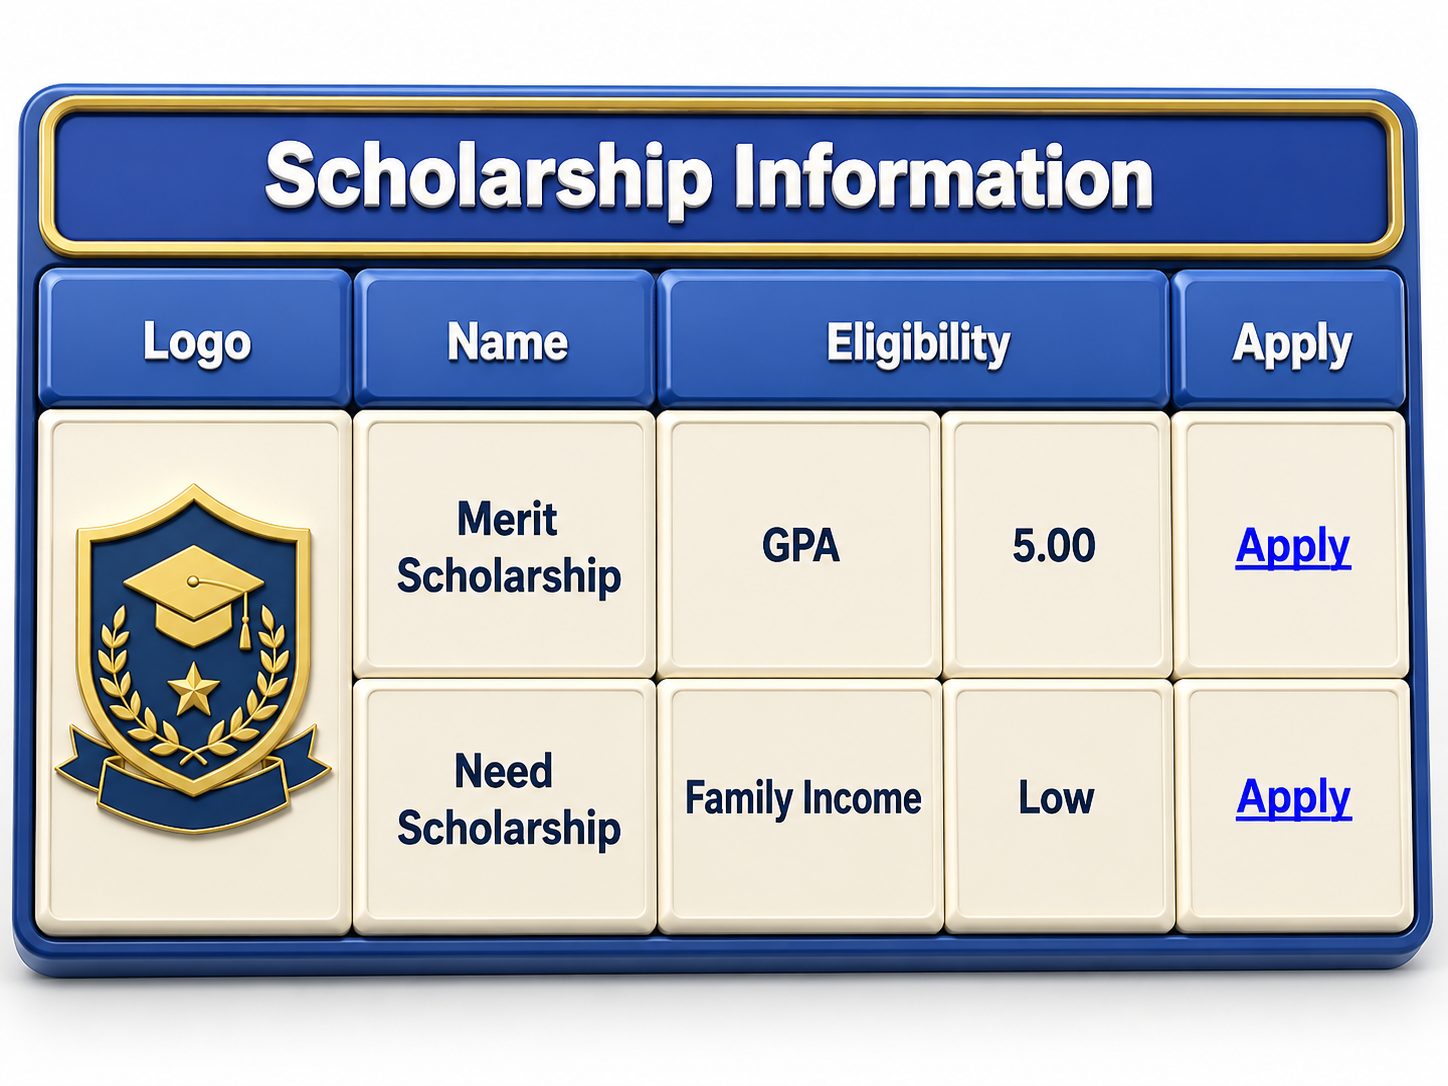
\includegraphics[width=0.95\linewidth,height=0.11\textheight,keepaspectratio]{chapters/Chapter04/topics/images/board_ex67_3d_scholarship_table.png}
}{
\fbox{\parbox{0.90\linewidth}{\centering\vspace{0.45cm}
\textbf{চিত্র}\\[3pt]
File: \texttt{chapters/Chapter04/topics/images/board\_ex67\_3d\_scholarship\_table.png}
\vspace{0.45cm}}}
}
\captionof{figure}{Scholarship Table with Logo, Link and Merged Eligibility}
\end{center}

\begin{keypointbox}{চিত্র ব্যাখ্যা}
Logo দুই scholarship row জুড়ে আছে; Eligibility heading দুই column জুড়ে আছে।
\end{keypointbox}

\begin{keypointbox}{চিত্র দেখে code লেখার ধাপ}
প্রথমে figure-এর total row ও column গুনবে। এরপর কোন cell একাধিক column জুড়ে আছে তা দেখে \texttt{colspan} এবং কোন cell একাধিক row জুড়ে আছে তা দেখে \texttt{rowspan} বসাবে। তারপর image, link, list বা nested table থাকলে সংশ্লিষ্ট tag cell-এর ভিতরে লিখবে।
\end{keypointbox}

\par\noindent{\color{purple!70!black}\bfseries\small কোড}\par\vspace{-4pt}
\begin{verbatim}
<!DOCTYPE html>
<html>
<head>
  <title>HTML Table Example</title>
</head>
<body>
<table border="1" cellspacing="0" cellpadding="6" align="center">
  <caption><b>Scholarship Information</b></caption>
  <tr>
    <th>Logo</th>
    <th>Name</th>
    <th colspan="2">Eligibility</th>
    <th>Apply</th>
  </tr>
  <tr>
    <td rowspan="2"><img src="scholarship.png" width="70" height="70" alt="Scholarship"></td>
    <td>Merit Scholarship</td>
    <td>GPA</td>
    <td>5.00</td>
    <td><a href="merit.html">Apply</a></td>
  </tr>
  <tr>
    <td>Need Scholarship</td>
    <td>Family Income</td>
    <td>Low</td>
    <td><a href="need.html">Apply</a></td>
  </tr>
</table>
</body>
</html>
\end{verbatim}
\vspace{-6pt}

\begin{keypointbox}{Board technique}
প্রথমে মোট row ও column গুনবে। তারপর কোন cell horizontal merge হলে \texttt{colspan} এবং vertical merge হলে \texttt{rowspan} ব্যবহার করবে। image-এর জন্য \texttt{<img>} এবং link-এর জন্য \texttt{<a>} tag ব্যবহার করবে।
\end{keypointbox}


\subsubsection{Example 68: Website Layout Table with Header, Sidebar, Image and Footer}

\begin{center}
\IfFileExists{chapters/Chapter04/topics/images/board_ex68_3d_webpage_layout_table.png}{
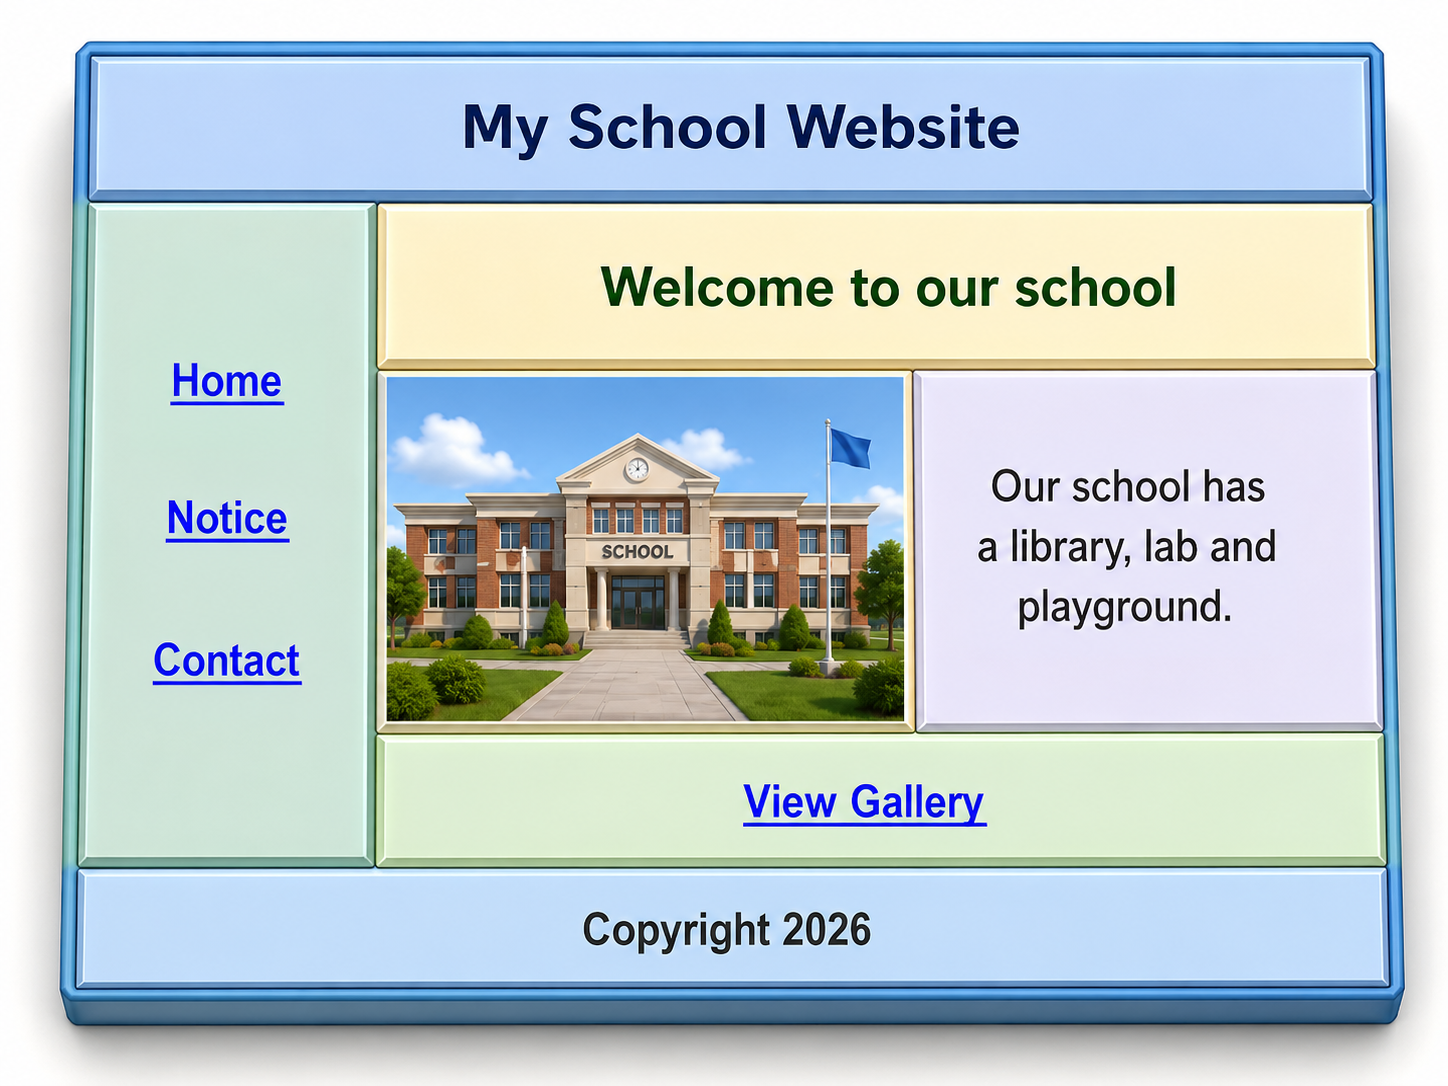
\includegraphics[width=0.95\linewidth,height=0.11\textheight,keepaspectratio]{chapters/Chapter04/topics/images/board_ex68_3d_webpage_layout_table.png}
}{
\fbox{\parbox{0.90\linewidth}{\centering\vspace{0.45cm}
\textbf{চিত্র}\\[3pt]
File: \texttt{chapters/Chapter04/topics/images/board\_ex68\_3d\_webpage\_layout\_table.png}
\vspace{0.45cm}}}
}
\captionof{figure}{Website Layout Table with Header, Sidebar, Image and Footer}
\end{center}

\begin{keypointbox}{চিত্র ব্যাখ্যা}
এটি webpage layout style table। Header ও footer colspan, sidebar rowspan, image এবং multiple links ব্যবহার করা হয়েছে।
\end{keypointbox}

\par\noindent{\color{purple!70!black}\bfseries\small কোড}\par\vspace{-4pt}
\begin{verbatim}
<!DOCTYPE html>
<html>
<head>
  <title>HTML Table Example</title>
</head>
<body>
<table border="1" cellspacing="0" cellpadding="8" align="center" width="600">
  <tr>
    <th colspan="3">My School Website</th>
  </tr>
  <tr>
    <td rowspan="3">
      <a href="home.html">Home</a><br>
      <a href="notice.html">Notice</a><br>
      <a href="contact.html">Contact</a>
    </td>
    <td colspan="2" align="center">Welcome to our school</td>
  </tr>
  <tr>
    <td><img src="school.jpg" width="150" height="90" alt="School"></td>
    <td>Our school has a library, lab and playground.</td>
  </tr>
  <tr>
    <td colspan="2" align="center"><a href="gallery.html">View Gallery</a></td>
  </tr>
  <tr>
    <td colspan="3" align="center">Copyright 2026</td>
  </tr>
</table>
</body>
</html>
\end{verbatim}
\vspace{-6pt}

\begin{keypointbox}{Board technique}
প্রথমে মোট row ও column গুনবে। তারপর কোন cell horizontal merge হলে \texttt{colspan} এবং vertical merge হলে \texttt{rowspan} ব্যবহার করবে। image-এর জন্য \texttt{<img>} এবং link-এর জন্য \texttt{<a>} tag ব্যবহার করবে।
\end{keypointbox}


\subsubsection{Example 69: College Contact Card with Nested Table, Image and Link}

\begin{center}
\IfFileExists{chapters/Chapter04/topics/images/board_ex69_3d_college_contact_nested.png}{
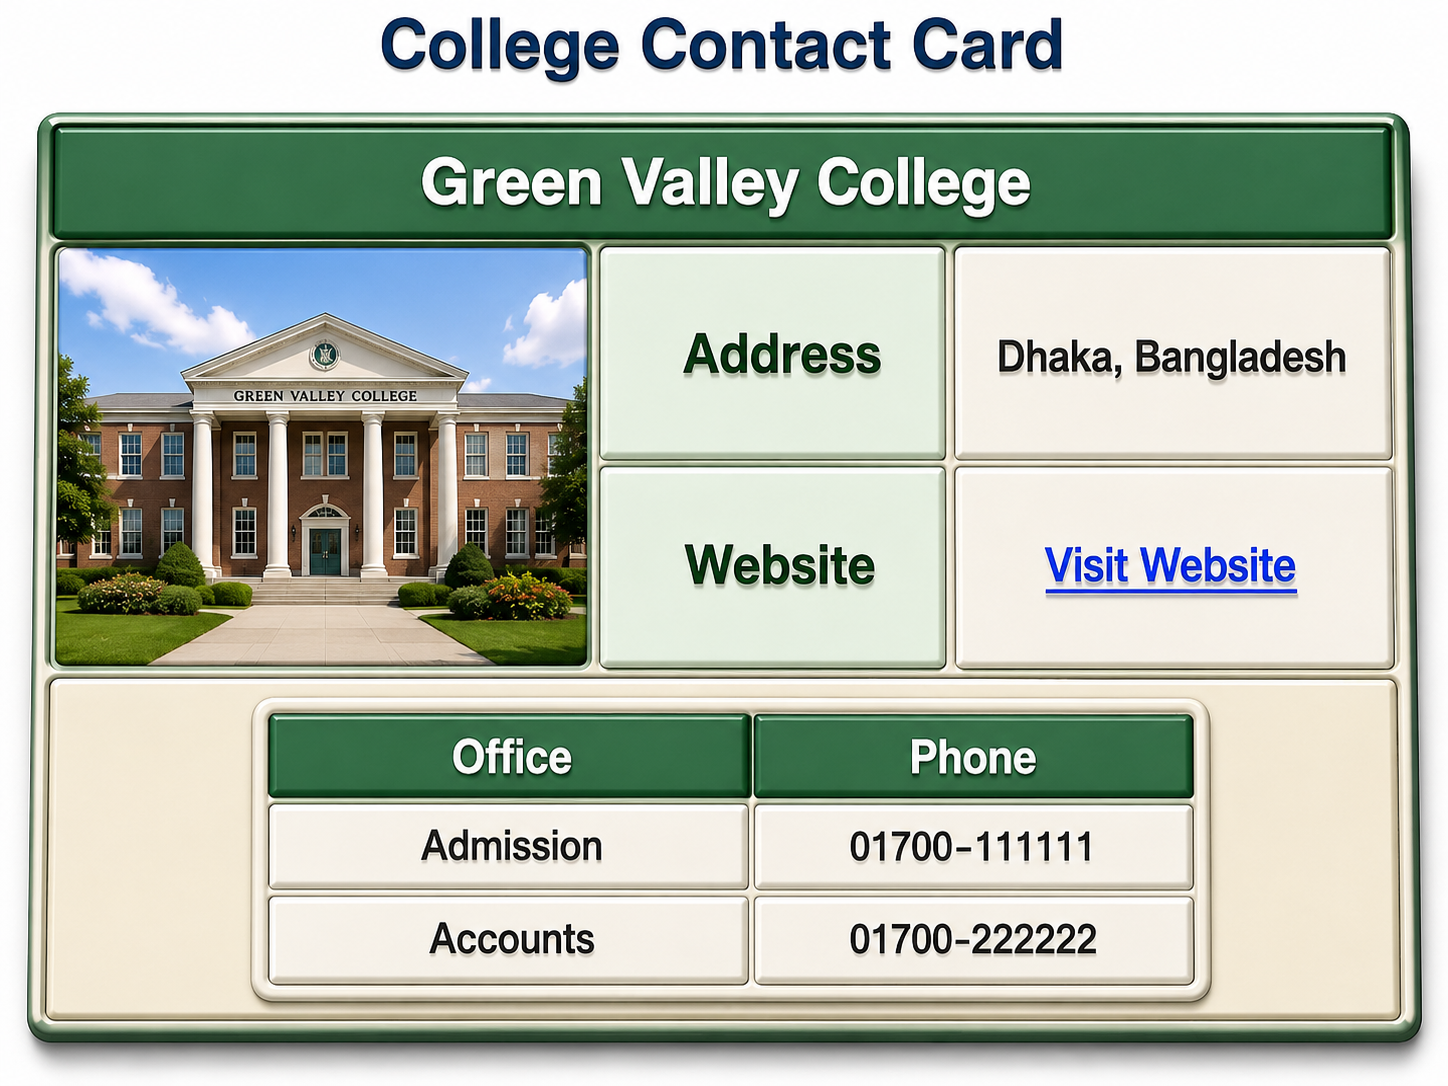
\includegraphics[width=0.95\linewidth,height=0.11\textheight,keepaspectratio]{chapters/Chapter04/topics/images/board_ex69_3d_college_contact_nested.png}
}{
\fbox{\parbox{0.90\linewidth}{\centering\vspace{0.45cm}
\textbf{চিত্র}\\[3pt]
File: \texttt{chapters/Chapter04/topics/images/board\_ex69\_3d\_college\_contact\_nested.png}
\vspace{0.45cm}}}
}
\captionof{figure}{College Contact Card with Nested Table, Image and Link}
\end{center}

\begin{keypointbox}{চিত্র ব্যাখ্যা}
এখানে outer table-এর ভিতরে nested table আছে। College image rowspan, title colspan এবং website hyperlink ব্যবহার করা হয়েছে।
\end{keypointbox}

\begin{keypointbox}{চিত্র দেখে code লেখার ধাপ}
প্রথমে figure-এর total row ও column গুনবে। এরপর কোন cell একাধিক column জুড়ে আছে তা দেখে \texttt{colspan} এবং কোন cell একাধিক row জুড়ে আছে তা দেখে \texttt{rowspan} বসাবে। তারপর image, link, list বা nested table থাকলে সংশ্লিষ্ট tag cell-এর ভিতরে লিখবে।
\end{keypointbox}

\par\noindent{\color{purple!70!black}\bfseries\small কোড}\par\vspace{-4pt}
\begin{verbatim}
<!DOCTYPE html>
<html>
<head>
  <title>HTML Table Example</title>
</head>
<body>
<table border="1" cellspacing="0" cellpadding="6" align="center">
  <caption><b>College Contact Card</b></caption>
  <tr>
    <th colspan="3">Green Valley College</th>
  </tr>
  <tr>
    <td rowspan="2"><img src="college.jpg" width="120" height="80" alt="College"></td>
    <td>Address</td>
    <td>Dhaka, Bangladesh</td>
  </tr>
  <tr>
    <td>Website</td>
    <td><a href="https://example.com">Visit Website</a></td>
  </tr>
  <tr>
    <td colspan="3">
      <table border="1" cellspacing="0" cellpadding="4" align="center">
        <tr>
          <th>Office</th>
          <th>Phone</th>
        </tr>
        <tr>
          <td>Admission</td>
          <td>01700-111111</td>
        </tr>
        <tr>
          <td>Accounts</td>
          <td>01700-222222</td>
        </tr>
      </table>
    </td>
  </tr>
</table>
</body>
</html>
\end{verbatim}
\vspace{-6pt}

\begin{keypointbox}{Board technique}
প্রথমে মোট row ও column গুনবে। তারপর কোন cell horizontal merge হলে \texttt{colspan} এবং vertical merge হলে \texttt{rowspan} ব্যবহার করবে। image-এর জন্য \texttt{<img>} এবং link-এর জন্য \texttt{<a>} tag ব্যবহার করবে।
\end{keypointbox}


\end{multicols}

\begin{recapbox}
এই ১৫টি mixed table practice-এ \texttt{rowspan}, \texttt{colspan}, image, hyperlink, list, nested table, caption, alignment এবং width—সব ধরনের গুরুত্বপূর্ণ HSC ICT table concept একসাথে cover করা হয়েছে। Exam-এ চিত্র দেখে code লেখার আগে structure analysis করাই সবচেয়ে গুরুত্বপূর্ণ।
\end{recapbox}

\subsection{চিত্র দেখে Table লেখার Final Checklist}

Board practical বা CQ-তে table-এর চিত্র দেওয়া থাকলে নিচের checklist ব্যবহার করলে ভুল কম হয়। এটি simple table, merged table, image/link/list-সহ table এবং nested table--সব ধরনের প্রশ্নে কাজে লাগে।

\begin{enumerate}
\item Table-এর নাম বা caption আছে কি না দেখবে।
\item Header row আছে কি না দেখবে।
\item Visible column সংখ্যা গুনবে।
\item Visible row সংখ্যা গুনবে।
\item Merged cell থাকলে আগে \texttt{rowspan} না \texttt{colspan} তা ঠিক করবে।
\item যে cell-এ image আছে সেখানে \texttt{<img>} এবং \texttt{alt} লিখবে।
\item যে cell-এ link আছে সেখানে \texttt{<a href="">} ব্যবহার করবে।
\item যে cell-এ list আছে সেখানে \texttt{<ol>} বা \texttt{<ul>} ব্যবহার করবে।
\item Nested table থাকলে inner table আলাদা indentation দিয়ে লিখবে।
\item শেষে সব \texttt{<table>}, \texttt{<tr>}, \texttt{<td>} tag close হয়েছে কি না মিলিয়ে দেখবে।
\end{enumerate}

\begin{keypointbox}{শেষ মুহূর্তের পরীক্ষা}
Code লেখা শেষ হলে প্রতিটি row আলাদা করে দেখবে: row-এর মোট column count figure-এর সাথে মিলছে কি না। \texttt{colspan="2"} মানে ওই cell দুই column-এর জায়গা নিয়েছে, তাই সেই row-তে একটি cell কম থাকবে। \texttt{rowspan="2"} মানে পরের row-তে ওই column-এর জন্য নতুন cell লিখতে হবে না।
\end{keypointbox}

\subsection{Board/Exam Focus}

\begin{boardbox}{বেশি গুরুত্বপূর্ণ}
\begin{itemize}
\item \texttt{<table>} tag table তৈরির জন্য ব্যবহৃত হয়।
\item \texttt{<tr>} row তৈরি করে।
\item \texttt{<th>} heading cell তৈরি করে।
\item \texttt{<td>} data cell তৈরি করে।
\item \texttt{<caption>} table-এর title দেয়।
\item \texttt{border} table border দেখায়।
\item \texttt{cellspacing} cell-এর মাঝের gap নির্ধারণ করে।
\item \texttt{cellpadding} cell-এর ভিতরের gap নির্ধারণ করে।
\item \texttt{rowspan} cell-কে vertical direction-এ merge করে।
\item \texttt{colspan} cell-কে horizontal direction-এ merge করে।
\item table-এর ভিতরে link, image, list এবং nested table ব্যবহার করা যায়।
\item চিত্র দেখে HTML table code লিখতে পারা খুব গুরুত্বপূর্ণ।
\end{itemize}
\end{boardbox}

\subsection{Exam-style Short Answer}

\begin{enumerate}
\item \textbf{HTML table কী?}\\
উত্তর: HTML document-এ তথ্যকে সারি ও কলাম আকারে প্রদর্শনের জন্য যে কাঠামো ব্যবহার করা হয়, তাকে HTML table বলে। Table তৈরির জন্য \texttt{<table>} tag ব্যবহার করা হয়।

\item \textbf{\texttt{<tr>} tag-এর কাজ কী?}\\
উত্তর: HTML table-এর একটি row বা সারি তৈরি করার জন্য \texttt{<tr>} tag ব্যবহার করা হয়।

\item \textbf{\texttt{<th>} ও \texttt{<td>} tag-এর পার্থক্য লেখ।}\\
উত্তর: \texttt{<th>} tag table-এর heading cell তৈরি করে এবং browser সাধারণত এর text bold ও center aligned করে দেখায়। অন্যদিকে \texttt{<td>} tag table-এর সাধারণ data cell তৈরি করে।

\item \textbf{\texttt{border} attribute-এর কাজ কী?}\\
উত্তর: HTML table-এর চারপাশে এবং cell-এর চারপাশে border বা রেখা প্রদর্শনের জন্য \texttt{border} attribute ব্যবহার করা হয়।

\item \textbf{\texttt{cellspacing} ও \texttt{cellpadding}-এর পার্থক্য লেখ।}\\
উত্তর: \texttt{cellspacing} cell থেকে cell-এর মাঝের gap নির্ধারণ করে। অন্যদিকে \texttt{cellpadding} cell-এর content এবং cell border-এর মাঝের ভিতরের gap নির্ধারণ করে।

\item \textbf{\texttt{rowspan} ও \texttt{colspan}-এর পার্থক্য লেখ।}\\
উত্তর: \texttt{rowspan} একটি cell-কে একাধিক row জুড়ে বিস্তৃত করে। \texttt{colspan} একটি cell-কে একাধিক column জুড়ে বিস্তৃত করে।

\item \textbf{Table-এর ভিতরে image বসানোর code লেখ।}\\
উত্তর: \texttt{<td><img src="photo.jpg" width="100" height="80" alt="Photo"></td>}

\item \textbf{Nested table কী?}\\
উত্তর: একটি table-এর কোনো cell-এর ভিতরে আরেকটি table তৈরি করলে তাকে nested table বলে।
\end{enumerate}

\subsection{Practice MCQ}

\begin{enumerate}
\item HTML-এ table তৈরির tag কোনটি?\\
ক) \texttt{<tr>} \quad খ) \texttt{<td>} \quad গ) \texttt{<table>} \quad ঘ) \texttt{<th>}

\item Table row তৈরি করতে কোন tag ব্যবহার হয়?\\
ক) \texttt{<td>} \quad খ) \texttt{<tr>} \quad গ) \texttt{<th>} \quad ঘ) \texttt{<caption>}

\item Table heading cell তৈরির tag কোনটি?\\
ক) \texttt{<td>} \quad খ) \texttt{<tr>} \quad গ) \texttt{<th>} \quad ঘ) \texttt{<br>}

\item Table data cell তৈরির tag কোনটি?\\
ক) \texttt{<td>} \quad খ) \texttt{<tr>} \quad গ) \texttt{<table>} \quad ঘ) \texttt{<hr>}

\item Table-এর border দেখাতে কোন attribute ব্যবহার করা হয়?\\
ক) \texttt{src} \quad খ) \texttt{href} \quad গ) \texttt{border} \quad ঘ) \texttt{target}

\item \texttt{cellpadding="5"} এর অর্থ কী?\\
ক) cell-এর ভিতরে content ও border-এর মাঝে 5 pixel space\\
খ) দুই cell-এর মাঝে 5 meter space\\
গ) table-এর height 5\\
ঘ) table-এর row সংখ্যা 5

\item \texttt{cellspacing} কোথায় space তৈরি করে?\\
ক) content ও border-এর ভিতরে \quad খ) cell ও cell-এর মাঝে \quad গ) image-এর ভিতরে \quad ঘ) hyperlink-এর পরে

\item দুইটি column merge করতে কোন attribute ব্যবহার হয়?\\
ক) \texttt{rowspan} \quad খ) \texttt{colspan} \quad গ) \texttt{cellpadding} \quad ঘ) \texttt{bgcolor}

\item দুইটি row merge করতে কোন attribute ব্যবহার হয়?\\
ক) \texttt{rowspan} \quad খ) \texttt{colspan} \quad গ) \texttt{align} \quad ঘ) \texttt{src}

\item Table-এর title দিতে কোন tag ব্যবহার হয়?\\
ক) \texttt{<title>} \quad খ) \texttt{<caption>} \quad গ) \texttt{<thead>} \quad ঘ) \texttt{<link>}

\item Image কোন tag দিয়ে table cell-এর ভিতরে বসানো যায়?\\
ক) \texttt{<a>} \quad খ) \texttt{<img>} \quad গ) \texttt{<ol>} \quad ঘ) \texttt{<tr>}

\item একটি table-এর cell-এর ভিতরে আরেকটি table বসালে তাকে কী বলে?\\
ক) outer table \quad খ) nested table \quad গ) image table \quad ঘ) child table
\end{enumerate}

\begin{boardbox}{MCQ Answer Key}
১-গ, ২-খ, ৩-গ, ৪-ক, ৫-গ, ৬-ক, ৭-খ, ৮-খ, ৯-ক, ১০-খ, ১১-খ, ১২-খ
\end{boardbox}

\subsection{CQ Practice}

\begin{practicebox}
\textbf{উদ্দীপক:} একটি webpage-এ Result Sheet table দেখাতে হবে। Table-এ border থাকবে, cell-এর ভিতরে ৫ pixel space থাকবে এবং cellগুলোর মাঝের gap থাকবে না। Table-এর প্রথম row-তে \texttt{Result Sheet} লেখা থাকবে এবং সেটি তিনটি column জুড়ে থাকবে।

\textbf{প্রশ্ন}\\
ক. HTML table কী?\\
খ. \texttt{<th>} ও \texttt{<td>} tag-এর কাজ লেখ।\\
গ. উদ্দীপকের জন্য HTML code লেখ।\\
ঘ. \texttt{border}, \texttt{cellspacing}, \texttt{cellpadding} ও \texttt{colspan} attribute-এর ব্যবহার বিশ্লেষণ কর।
\end{practicebox}

\subsubsection{গ. কোড}

\begin{examplebox}{কোড}
\begin{verbatim}
<!DOCTYPE html>
<html>
<head>
  <title>Result Table</title>
</head>
<body>
  <table border="1" cellspacing="0" cellpadding="5">
    <tr>
      <th colspan="3">Result Sheet</th>
    </tr>
    <tr>
      <th>Roll</th>
      <th>Name</th>
      <th>GPA</th>
    </tr>
    <tr>
      <td>101</td>
      <td>Rafi</td>
      <td>5.00</td>
    </tr>
    <tr>
      <td>102</td>
      <td>Sakib</td>
      <td>4.75</td>
    </tr>
  </table>
</body>
</html>
\end{verbatim}
\end{examplebox}

\subsubsection{ঘ. বিশ্লেষণ}

\texttt{border="1"} table ও cell-এর চারপাশে border দেখায়। \texttt{cellspacing="0"} cellগুলোর মাঝের gap দূর করে। \texttt{cellpadding="5"} cell-এর ভিতরে content ও border-এর মাঝে ৫ pixel space তৈরি করে, ফলে table পড়তে সহজ হয়। \texttt{colspan="3"} প্রথম heading cell-কে তিনটি column জুড়ে বিস্তৃত করে, তাই \texttt{Result Sheet} title পুরো table-এর উপর দেখা যায়।

\subsection{Common Mistake}

\begin{mistakebox}{সাধারণ ভুল}
\begin{itemize}
\item \texttt{<table>} tag close না করা।
\item \texttt{<tr>} ছাড়া সরাসরি \texttt{<td>} লেখা।
\item heading cell-এ \texttt{<td>} ব্যবহার করা, যেখানে \texttt{<th>} ভালো।
\item \texttt{<td>}-এর spelling ভুল করে \texttt{<tb>} লেখা।
\item \texttt{cellpadding} ও \texttt{cellspacing} গুলিয়ে ফেলা।
\item \texttt{rowspan} ও \texttt{colspan} উল্টো ব্যবহার করা।
\item border না দিলে table-এর রেখা দেখা যাবে না--এটা ভুলে যাওয়া।
\item table row ও column সংখ্যা figure-এর সাথে না মেলানো।
\item \texttt{<caption>} ভুল জায়গায় লেখা। Caption সাধারণত \texttt{<table>} tag-এর ভিতরে, প্রথম row-এর আগে লেখা হয়।
\item table-এর ভিতরে image/link/list লিখতে syntax ভুল করা।
\item image tag-এ \texttt{src} ভুল দেওয়া বা image file একই folder-এ না রাখা।
\item nested table-এর closing tag ঠিকমতো না দেওয়া।
\end{itemize}
\end{mistakebox}

\subsection{১ মিনিটে রিভিশন}

\begin{recapbox}
Table তৈরি হয় row ও column দিয়ে। \texttt{<table>} পুরো table তৈরি করে, \texttt{<tr>} table row তৈরি করে, \texttt{<th>} heading cell তৈরি করে এবং \texttt{<td>} data cell তৈরি করে। \texttt{border} table border দেখায়, \texttt{cellspacing} cell-এর মাঝের gap নিয়ন্ত্রণ করে এবং \texttt{cellpadding} cell-এর ভিতরের gap নিয়ন্ত্রণ করে। \texttt{<caption>} table-এর title দেয়। \texttt{rowspan} vertical merge এবং \texttt{colspan} horizontal merge করে। Table cell-এর ভিতরে text, link, image, list ও nested table রাখা যায়। HSC CQ-তে table চিত্র দেখে code লেখা খুব গুরুত্বপূর্ণ।
\end{recapbox}










